%% ----------------------------------------------------------------
%% thesis.tex -- MAIN FILE (the one that you compile with LaTeX)
%% ---------------------------------------------------------------- 

% Set up the document
\documentclass[a4paper, 11pt, oneside]{thesis}  % Use the "Thesis" style, based on the ECS Thesis style by Steve Gunn

\makeglossaries
\loadglsentries{glossary}

%% ----------------------------------------------------------------
\begin{document}

\frontmatter      % Begin Roman style (i, ii, iii, iv...) page numbering

% Set up the Title Page
\title  {Analysis and Coordination of Mixed-criticality Cyber-physical Systems}
\authors  {\texorpdfstring
            {\href{simon.maurer@protonmail.ch}{Simon Maurer}}
            {Simon Maurer}
            }
\addresses  {\groupname\\\deptname\\\univname}  % Do not change this here, instead these must be set in the "Thesis.cls" file, please look through it instead
\date       {\today}
\subject    {}
\keywords   {}

\maketitle
%% ----------------------------------------------------------------

\setstretch{1.3}  % It is better to have smaller font and larger line spacing than the other way round

% Define the page headers using the FancyHdr package and set up for one-sided printing
\fancyhead{}  % Clears all page headers and footers
\rhead{\thepage}  % Sets the right side header to show the page number

\pagestyle{fancy}  % Finally, use the "fancy" page style to implement the FancyHdr headers

\addcontentsline{toc}{chapter}{Preface}
\cleardoublepage  % End of the Abstract
% %% ----------------------------------------------------------------
% % Declaration Page required for the Thesis, your institution may give you a different text to place here
% \addcontentsline{toc}{section}{Declaration of Authorship}
% \Declaration{
%     I, Simon Maurer, declare that this thesis titled, `Coordination of Mixed-criticality Cyber-physical Systems' and the work presented in it are my own. I confirm that:

%     \begin{itemize}
%         \item[\tiny{$\blacksquare$}] This work was done wholly or mainly while in candidature for a research degree at this University.
%         \item[\tiny{$\blacksquare$}] Where any part of this thesis has previously been submitted for a degree or any other qualification at this University or any other institution, this has been clearly stated.
%         \item[\tiny{$\blacksquare$}] Where I have consulted the published work of others, this is always clearly attributed.
%         \item[\tiny{$\blacksquare$}] Where I have quoted from the work of others, the source is always given. With the exception of such quotations, this thesis is entirely my own work.
%         \item[\tiny{$\blacksquare$}] I have acknowledged all main sources of help.
%         \item[\tiny{$\blacksquare$}] Where the thesis is based on work done by myself jointly with others, I have made clear exactly what was done by others and what I have contributed myself.\\
%     \end{itemize}

%     Signed:\\
%     \rule[1em]{25em}{0.5pt}  % This prints a line for the signature

%     Date:\\
%     \rule[1em]{25em}{0.5pt}  % This prints a line to write the date
% }
% \clearpage  % Declaration ended, now start a new page

%% ----------------------------------------------------------------

% The Abstract Page
% \addcontentsline{toc}{section}{Abstract}
\addtotoc{Abstract}
\abstract{
    A \gls{cps} can be described as a network of interlinked, concurrent computational components that interact with the physical world.
    Such a system is usually of reactive nature and must satisfy strict timing requirements to guarantee a correct behaviour.
    The components can be of mixed-criticality which implies different progress models and communication models, depending whether the focus of a component lies on predictability or resource efficiency.

    In this dissertation I present a novel approach that bridges the gap between stream processing models and \glspl{lts}.
    The former offer powerful tools to describe concurrent systems of, usually simple, components while the latter allow to describe complex, reactive, components and their mutual interaction.
    In order to achieve the bridge between the two domains I introduce the novel \gls{lts} \emph{\gls{sia}} that allows to model the interaction protocol of a process via its interface and to incrementally compose simple processes into more complex ones while preserving the system properties.
    Exploiting these properties I introduce an analysis to identify permanent blocking situations in a network of composed processes.
    \Glspl{sia} are wrapped by the novel component-based coordination model \emph{\gls{pnsc}} that allows to describe a network of concurrent processes where multiple communication models and the co-existence and interaction of heterogeneous processes is supported due to well defined interfaces.

    The work presented in this dissertation follows a holistic approach which spans from the theory of the underlying model to an instantiation of the model as a novel coordination language, called \emph{\gls*{smx}}.
    The language uses network operators to compose networks of concurrent processes in a structured and hierarchical way.
    The work is validated by a prototype implementation of a compiler and a \gls{rts} that allows to compile a \gls*{smx} program and execute it on a platform with support for ISO C, POSIX threads, and a Linux operating system.
}
\cleardoublepage  % End of the Abstract
%% ----------------------------------------------------------------

\setstretch{1.3}  % Reset the line-spacing to 1.3 for body text (if it has changed)

% The Acknowledgements page, for thanking everyone
% \addcontentsline{toc}{section}{Acknowledgements}
\addtotoc{Acknowledgements}
\acknowledgements{
    First, my gratitude goes to the University of Hertfordshire for providing the funding and infrastructure for my PhD and for giving me the opportunity to start a career in academia.

    I would like to thank my primary supervisor and research mentor Dr~Raimund Kirner for the support of my PhD and related research.
    I am grateful for his commitment to provide me with guidance even late at night or on weekends.
    His broad knowledge and his patience were a huge help throughout the whole of the PhD.

    Further, I would like to express my gratitude to Dr~Olga Tveretina, my secondary supervisor, for her valuable inputs and her mental support.
    My thanks also go to Dr~Prof~Alex Shafarenko, leader of the research group \groupname, for his invaluable feedback.

    I thank Giovina for her patience and her interest in abstract topics that are not hers.
    Her cheerful and supportive attitude were a big help throughout this project and I am ever grateful to her for leading me onto this path.
    Her hilarious personifications of certain aspects of my work, complete with pictures and all, is only one of many examples of her brilliant way of supporting me.

    Although I do not know these people personally I want to give a shout out to Randall Munroe for his book "Thing Exaplainer - Complicated Stuff in Simple Words", showing that complicated things can be explained with only a 1000 words and Linda Liukas, for her book "Hello Ruby", advocating the fact that computer science is not as difficult as common belief suggests and that it can be taught to anyone.

    Last but not least, I want to thank my family and friends from abroad for their continuous support and their willingness to pay us visit on a regular basis.
    % I cannot stress enough how much I appreciated 
}
\cleardoublepage  % End of the Acknowledgement
%% ----------------------------------------------------------------

\pagestyle{fancy}  %The page style headers have been "empty" all this time, now use the "fancy" headers as defined before to bring them back

\setstretch{1.0}  % It is better to have smaller font and larger line spacing than the other way round
%% ----------------------------------------------------------------
\lhead{\emph{Contents}}  % Set the left side page header to "Contents"
% \addcontentsline{toc}{section}{Contents}
\addtotoc{Contents}
\tableofcontents  % Write out the Table of Contents
\cleardoublepage  % End of the Content

%% ----------------------------------------------------------------
\lhead{\emph{List of Figures}}  % Set the left side page header to "List if Figures"
% \addcontentsline{toc}{section}{List of Figures}
\addtotoc{List of Figures}
\listoffigures  % Write out the List of Figures
\cleardoublepage  % End of the Figures

%% ----------------------------------------------------------------
\lhead{\emph{List of Definitions}}  % Set the left side page header to "List of Tables"
\renewcommand{\listtheoremname}{List of Definitions}
% \addcontentsline{toc}{section}{\listtheoremname}
\addtotoc{\listtheoremname}
% \listoftheorems[ignoreall,show=definition]  % Write out the List of Definitions
\listoftheorems  % Write out the List of Definitions
\cleardoublepage  % End of the Definitions

%% ----------------------------------------------------------------
\lhead{\emph{Acronyms}}  % Set the left side page header to "Abbreviations"
% \addcontentsline{toc}{section}{Acronyms}
\addtotoc{Acronyms}
\printacronyms
\cleardoublepage  % End of the Acronyms

% End of the pre-able, contents and lists of things
% Begin the Dedication page

\setstretch{1.3}  % Return the line spacing back to 1.3

\addtocontents{toc}{\vspace{3em}}  % Add a gap in the Contents, for aesthetics

%% ----------------------------------------------------------------
\mainmatter	  % Begin normal, numeric (1,2,3...) page numbering
\pagestyle{fancy}  % Return the page headers back to the "fancy" style
\lhead{\emph{\leftmark}}  % Clears the left side page header

% Include the chapters of the thesis, as separate files
% Just uncomment the lines as you write the chapters

\glsresetall
% -*-mode: Latex-*-
% !TEX root = thesis.tex
% paper: ...
% authors: simon maurer
%
% file: introduction.tex
% contents: introduction to the thesis
% Sccs-Id: %W% %G%
\chapter{Introduction}
\label{chap_intro}
Nowadays, with microcontrollers getting smaller and more efficient, computing is becoming more and more pervasive in our everyday life.
This is achieved by embedding computer devices in physical objects such that the computing devices interact with the physical world.
Such systems are called \glspl{cps}.
A \gls{cps} is a reactive system that senses its environment (the physical world), performs a computation on a computational entity (this can be anything from a simple embedded device to a large scale distributed system), and then actuates on the environment according to the computations.
The actuation on the environment causes the environment to change which, in turn, is detected by the sensors and the computation is performed with the new dataset.
Typically, this reactive loop is time-critical and is executed as long as the system is running.
In contrast to a traditional embedded system, \ie a time-critical system, dedicated to a single hardware platform, a \gls{cps} tends to be an assembly of networked subsystems where some subsystems interact with the physical world and some may be purely computational.

Examples of \glspl{cps} can be found in the domain of automotive vehicles (\eg anti-lock braking system, adaptive cruise control, electronic stability control, platooning), avionic vehicles (\eg flight control systems, black box, pressure control), or smart spaces (\eg intelligent highway control, building control), to name only a few.

Because of the direct interaction of \glspl{cps} with the physical world, it is often crucial to respect timing requirements imposed by the physical world to guarantee a correct behaviour of the system.
In case of critical applications such as nuclear power plants, avionic systems, or cars, huge efforts are made to verify the correct behaviour of the application.
The main difference between critical systems and best-effort systems is that critical systems are designed for the worst case whereas best-effort systems are designed for the average case.
Henzinger and Sifakis argue that over time, this difference led to a gap between the models employed in the two domains and that the gap is continuing to widen~\cite{henzinger2006}.
Due to the difference of the employed models, critical and non-critical applications tend to be physically separated and run on dedicated hardware platforms.
This is a problem because with the evolution of hardware towards multi/many-core architectures, there is the interest to integrate components with different criticality requirements on the same platform.
Such systems are typically called mixed-criticality systems~\cite{burns2016}.
What adds further to the challenge of integrating \glspl{cps} on a multi/many-core architecture is that \glspl{cps} are often heterogeneous in the sense that several applications from different domains with different characteristics must coexist or interact with each other~\cite{eker2003}.
Eker \etal address this challenge by assembling multiple models, each suitable for its specific application domain, in one framework~\cite{eker2003}.
Others argue that one meta model, allowing to describe and compose heterogeneous systems, is more beneficial because it provides a better ground for a meaningful analysis of the system~\cite{henzinger2006, rajkumar2010, castrillon2015}.
% This is also referred to as model-based design.

Another challenge is the inherent concurrency of \glspl{cps}~\cite{lee2008}.
Streaming networks are well-recognised for coping with concurrent systems~\cite{stephens1997}.
They consist of processing nodes (often called filters) connected via communication channels where a channel is connected to a single producer node and a single consumer node.
This property of streaming networks, combined with the implicit synchronisation of producers and consumers due to a blocking channel access, allows to tame the complexity of concurrent systems which makes them also an interesting paradigm to apply to \glspl{cps}.
However, current streaming models (\eg~\cite{thies2002, lee2003, grelck2010}) tend to rely on the possibility that a system can be decomposed into transformational components such that the behaviour of a component can be described as a pure function.
Such a decomposition makes it easier to understand component dependencies and allows to analyse the system, \eg for schedulability~\cite{lee1987} or deadlocks~\cite{zhou2006}.
However, given that \glspl{cps} are often systems of reactive nature, such a decomposition is difficult~\cite{harel1985}.

An interesting approach where no decomposition in transformational components is required are interface theories~\cite{deAlfaro2001} which allow to describe components with arbitrary behaviour by their interfaces and build complex components out of simple ones by composition.
Several interface models have been proposed to describe communication compatibility between components~\cite{deAlfaro2001a, larsen2006, hennicker2015} as well as additional properties such as modalities~\cite{larsen2007}, resource usage~\cite{chakrabarti2003, thiele2006}, or timing constraints~\cite{dealfaro2002, henzinger2006a}.
However, these models do not target streaming networks and lack the capability of describing the blocking semantics of message passing in streaming networks.

In this dissertation I introduce a novel automata-based interface description model, called \gls{sia}, that allows to describe the interaction protocol of processes with their environment.
\Glspl{sia} are suitable to describe the blocking semantics of \gls{kpn}-based~\cite{kahn1974} streaming networks and thus serve as a powerful tool to bridge the gap between \gls{lts} and stream processing.
An incremental composition operation allows to build complex processes out of simple ones.
A novelty of the \gls{sia} model is that it allows to identify permanent blocking situations (\eg deadlocks) in a composed network due to the blocking semantics of the model.
The inspiration for the \gls{sia} model stems from \glspl{ia}~\cite{deAlfaro2001a}.
The blocking semantics of the here presented \glspl{sia} differs fundamentally from the blocking semantics of \glspl{ia}.
This enables \glspl{sia} to describe process networks where processes interact with synchronous communication, \eg~stream processing applications.

I further introduce a novel component-based model, called \gls{pnsc} that serves as a wrapper for \glspl{sia} and allows to model an assembly of reactive processes, \ie processes capable of consuming and producing streams of infinite length.
I extend the model to support the coexistence and interaction of processes with an event-triggered and a time-triggered execution scheme.
In the former case, sporadically occurring events are causing a subsystem to perform its computation while in the latter case a fixed schedule imposes time instances when a subsystem is performing its computation.
There are application domains where both models are required (\eg automotive domain) but the two models are often used in limited ways to just co-exist but do not directly interact with each other (\eg~\cite{ferreira2002, steiner2011, obermaisser2006}).
The problem is that interaction may cause interference from a subsystem of low criticality towards a subsystem of high criticality which must be avoided.
A novelty of the extended \gls{pnsc} model is that it allows not only the co-existence of the two triggering semantics in the same system but also allows interaction between time-triggered subsystems and event-triggered subsystems.
The key point is to guarantee that the event-triggered subsystem, having a lower criticality level, is not interfering with the time-triggered subsystem of higher criticality.
Further, the model allows to use the same mechanism to avoid interference from a lower critical event-triggered subsystem to a higher critical event-triggered subsystem.
Two time-triggered subsystems do not interfere with each other out of construction~\cite{kopetz2002}, independent of their criticality level.

To provide control on communication bandwidth usage, the model allows to limit the communication rate of a process to an upper bound.
This is achieved with a novel approach of controlling message passing between processes with different consequences depending on the message semantics.

A challenge related to the inherent concurrency of \glspl{cps} is the efficient execution of concurrent systems on multi-core hardware platforms.
With the ever growing capabilities of integrated circuits due to the persistence of Moore's law, software engineers face the challenge to design, develop, and maintain complex software systems that exploit the available computation power.
As a consequence of reaching the power wall through frequency scaling~\cite{pollack1999}, parallel hardware architectures have been designed.
Even in the domain of embarrassingly parallelisable applications where it is easy to split the computation load in a large number of independent computational chunks due to lack of data or code dependencies, parallelization remains not a simple task because of the tight coupling between hardware and software (\eg efficient use of memory hierarchy) and the inherent difficulty of debugging parallel code.
Nowadays, there are tools, libraries, and languages available that help to cope with some of the problems.
In the domain of Big Data on large scale distributed systems examples are Hadoop\footnote{\url{http://hadoop.apache.org/}}, HPCC\footnote{\url{https://hpccsystems.com/}}, and Hydra\footnote{\url{https://github.com/addthis/hydra}}.
For shared memory multi-core architectures some examples are Cuda\footnote{\url{http://www.nvidia.com/object/cuda_home_new.html}}, OpenMP\footnote{\url{http://www.openmp.org/}}, and TBB\footnote{\url{https://www.threadingbuildingblocks.org/}}.

However, multi- and many-core processor architectures have emerged to a broad variety of application fields, including \glspl{cps}, where it is hard to identify potential blocks that can exhibit parallelism due to dependencies between tasks and, especially, due to the reactive nature of \glspl{cps}.
In their survey on programming solutions for multicore architectures in the domain of \glspl{cps}, Castrillon \etal note that even though achievements were made in academia, in industry, \gls{cps} software development for parallel architectures remains mostly manual~\cite{castrillon2015}.
A reason for this is that industry often relies on legacy code that may include system libraries or multiple layers of mixed languages which is often ignored by academic solutions (\eg introducing a new language requires industry to rewrite lots of legacy source code in the new language which they may be hesitant to do).

To cope with concurrency in applications, programming languages either incorporate models (\eg Actor model~\cite{agha1985} in Scala, \gls{csp}~\cite{hoare1978} in Ada) or libraries are provided (Open \gls{mpi}~\cite{open-mpi}) to simplify design, development, and maintainability of the application.
While such models certainly help to structure the code and enforce good practices in parallel programming, it is still up to the programmer to separate between coordinational and computational aspects of the program.
While an expert in a certain application domain - a \emph{domain expert} - is very adept in solving problems and working with models related to this domain, it is rarely his or her expertise to cope with the inherent problems of concurrency and parallelization.

An interesting approach to solve this problem is to separate the different concerns of an application, as proposed by Gelernter and Carriero in~\cite{gelernter1992}.
The main idea is to separate the concerns of computation and coordination by using a coordination language in addition to a programming language.
This allows the domain expert to choose a language that suits his needs to program computational blocks which are then linked together, potentially by another person, using a coordination language based on a model that is suitable to cope with concurrency.
This clear separation of concerns is an intriguing concept, especially for interdisciplinary application fields where experts from different domains work together.
As \glspl{cps} tend to describe applications in interdisciplinary fields, a clear separation of concerns is desirable.

In this dissertation I introduce a new coordination language, called \gls*{smx}, that is based on the \gls{pnsc} model, also introduced in this thesis.
While \gls*{smx} is an instantiation of the \gls{pnsc} model, the language provides more than just concrete syntax for the model:
\Gls*{smx} allows to describe a network of processes in a structured and hierarchical manner due to its usage of network composition operators.
This is inspired by the coordination language \gls*{snet}~\cite{grelck2010} which allows to describe networks of pure components.
The novelty of \gls*{smx} is that while it is based on the stream processing paradigm it retains the capability of describing \glspl{cps} where components are hard to decompose due to the reactive nature of \gls{cps}.
\Gls*{smx} is an exogenous coordination language where the coordinated components are unaware of the coordination exert on them~\cite{arbab2006}.

This dissertation describes a holistic approach, reaching from the underlying theory of the coordination model to an instantiation of the model in the form of a language and a prototype toolchain that allows to compile \gls*{smx} code into an executable C program, check the program for permanent blocking, and link it with C implementations of \gls{pnsc} processes.
The resulting application can be executed on a platform with support for ISO C, POSIX threads, and a Linux operating system.


%==============================================================================
\section{Thesis and Research Questions}
\label{sect_intro_question}
In this section I present the thesis this dissertation aims to maintain and several research questions that guided me through my research.
As described in the beginning of this chapter, my work aims at using models from different fields, namely stream processing and interface theory, and adapt the models in such a way that they are applicable for \glspl{cps}.
Consequently, I formulate my thesis as follows:
\begin{center}
    \rule[5mm]{\textwidth}{0.4pt}
    \parbox{0.8\textwidth}{
    \centering
        \emph{It is possible to bridge the gap between stream processing and \acrfullpl{lts} for complex components.}
    }
    \rule[-2mm]{\textwidth}{0.4pt}
\end{center}

In the following I will describe several research questions that focus on sub-aspects of the thesis and help to dissect each aspect independently.
I first ask a general question about coordination models to then refine it with three more precise questions:

\paragraph*{How to coordinate mixed-criticality CPSs?} \hfill

To answer this question, as a first step, it is crucial to identify properties of \glspl{cps} and understand how they relate to coordination aspects.
A mixed-criticality \gls{cps} is an assembly of networked subsystems with strong and weak coupling between them.
Some of the subsystems are critical systems, \ie of high criticality, some are best-effort systems, \ie of low criticality.
The coupling between the different subsystems is of various degrees.
Critical subsystems tend to have a weak coupling with other subsystems to prevent mutual interference while best-effort systems tend to be strongly coupled.
A coordination model for a mixed-criticality \gls{cps} must be able to model these various degrees of coupling between subsystems while providing guarantees of correctness of the overall behaviour of the system.

To refine the research question I ask two follow-up questions centring around the coupling of subsystems.
A third follow-up question focuses on coordination languages and the implication of reactive components on a language.

\paragraph*{What are suitable interfaces for reactive components with strong coupling to ensure correct behaviour of a system of such components assembled in a network?} \hfill

A main property of a component that supports reactive behaviour is that it must be able to cope with infinite streams, \ie potentially run infinitely.
Due to this property, a component must support to read an input as a reaction to writing an output.
This is because of a potential coupling between the output and the input through the environment.
This must be reflected in the interface describing the component.
In this dissertation I introduce the automata-based model \gls{sia} that allows to describe the interaction of a component with its environment.
\Glspl{sia} are based on a strict blocking semantics, modelling synchronous communication, which allows to describe streaming applications and their inherent strong coupling between components.
The \gls{sia} model allows the composition of simple components into more complex ones while preserving the blocking semantics.
I further introduce an analytic method, based on the \gls{sia} model, to detect situations where components are blocking indefinitely, \eg deadlock situations.

% A related but more general topic is discussed by Henzinger and Sifakis~\cite{henzinger2006}.
% They observed that the gap between engineering methodologies for critical systems and best-effort systems is widening.
% As a solution to bridge this gap, they proposed to unify heterogeneous systems under one meta-model that allows the composition of components while preserving properties.
% This same principle holds for coordination models for \glspl{cps} where the focus lies on communication and synchronisation.

% \emph{What are suitable coordination elements to support time-criticality in \glspl{cps}?}

% Guarantees on timing requirements create a tight bound between hardware and software and require a system to be predictable and analysable.
% Interfaces have to be provided that allow to perform model checking and verification processes on the subcomponents of the system.
% In addition, the model needs to provide facilities to annotate individual subcomponents with timing requirements.\\

\paragraph*{What are suitable interfaces for CPSs to integrate subsystems with different criticality levels?} \hfill

In contrast to a strong coupling, addressed in the previous question, a weak coupling allows to ensure the system correctness based on the component correctness.
The focus of this question lies on the interaction of subsystems with different degrees of coupling.
A main challenge of a mixed-criticality system is to allow multiple subsystems with different criticality levels to co-exist on the same platform or even to interact with each other.
The challenge of such a configuration is to assure that the subsystems with lower criticality levels do not interfere with subsystems of higher criticality levels.
In this dissertation I introduce \glspl{cci} that allow to selectively implement a weak coupling between two components and prevent such an interference.

\paragraph*{What are the implications of reactive components on an exogenous coordination language?} \hfill

The interaction of subsystems in a \gls{cps} is often based on reactive data processing where the environment imposes a link between the inputs and outputs of the component.
A reactive component is hard to decompose because reactive components tend to rely on persistent state and internal synchronisation points.
Due to this, simple and intuitive language primitives are required to describe reactive communication patterns in a structured way, such as chained components with mutual bi-directional interaction, without loosing in terms of locality.
I adopt the notion of network operators to describe a network of reactive components.
Different types of operators allow to describe a network in a structured and hierarchical manner by keeping information local.


%==============================================================================
\section{Contributions}
\label{sect_intro_contribution}

To illustrate the contribution of this dissertation, \Fig{\ref{fig_trinity}} provides a simplistic overview of related work and the gap between research fields that this dissertation aims to bridge.
In the figure, three circles represent three aspects that tend to be part of a \gls{cps}.
Each circle is associated with a model that allows to describe particular properties of each aspect and tackle the challenge they pose for modelling \glspl{cps}.
\begin{itemize}
    \item \Glspl{cps} tend to be \emph{concurrent} due to the fact that they interact with the physical world which is inherently concurrent~\cite{lee2008}.
        In this work, concurrency aspects are tackled with a stream processing model which provides inherent synchronisation between interacting components.
    \item \Glspl{cps} tend to be \emph{heterogeneous} with respect to multiple aspects such as mixed-criticality~\cite{burns2016}, different timing
        semantics~\cite{kopetz2011}, or different underlying theoretical models~\cite{eker2003}.
        In this dissertation I focus on mixed-criticality aspects and different timing semantics and use well defined communication interfaces, called \glspl{cci}, to control the interaction between components.
    \item \Glspl{cps} tend to be \emph{reactive} systems with complex interacting components which are hard to decompose~\cite{harel1985}.
        In order to support complex components in a stream processing model I introduce the novel \gls{sia} model, an analysable component abstraction.
\end{itemize}

Further, the figure shows a few examples of related work, prominent representatives of their domain, that are placed in the circles or the intersection of two circles to illustrate which aspects of \glspl{cps} are covered by their respective model.
The symbolic dial, surrounding the three circles, represents the time-criticality aspect of \glspl{cps}.
Of the represented models only the names that are not greyed-out support some sort of control over timing behaviour.
The figure illustrates a clear gap between reactive systems with support for complex components and stream processing models.
This gap is filled by the work presented in this dissertation, namely the \gls{pnsc} model and the extension of the model.

%------------------------------------------------------------------
\begin{figure}[bht]
    \TopFigSpace
    \vspace{2mm}
    \centering
    \includegraphics[width=10cm]{fig/trinity.pdf}
    \CaptionFigSpace
    \vspace{2mm}
    \caption{A simple schematic representation of properties of \glspl{cps} and how the novel \gls{pnsc} model bridges the gap between stream processing and \gls{lts} for complex componets.}
    \label{fig_trinity}
    \BotFigSpace
\end{figure}
%------------------------------------------------------------------

The work described in this dissertation provides the following novelties and contributions:
\begin{itemize}
    \item introduction of a novel exogenous, component-based coordination model, called \gls{pnsc}, that allows to describe networks of processes, communicating through sporadic message passing.
        The novelty of the model is an \gls{lts}, called \gls{sia}, first introduced in this dissertation, that allows to capture the blocking semantics of interacting processes.
        The model allows to describe processes with persistent state and internal synchronisation points.
        These are properties that fit well with the requirements of \glspl{cps} which tend to be networks of reactive components.
        A composition operator allows to compose processes while preserving the properties of blocking communication.
    \item extension of the novel \gls{pnsc} model.
        The extensions have no influence on the behavioural aspect of a process which preserves the exogenous coordination property of the \gls{pnsc} model.
        The extensions provide support for
        \begin{itemize}
            \item mixed-criticality systems through selective communication decoupling to prevent unwanted interference between processes.
                The extension integrates seamlessly with \glspl{sia} which are used to describe the communication decoupling mechanism.
            \item multiple process execution schemes in a process network.
                This is achieved by using the communication decoupling mechanism in conjunction with clock signals to enforce a time-triggered process execution on a subset of processes.
                The model allows to enforce time-triggered communication on individual processes or on a network of processes.
            \item rate-controlled event-triggered communication.
                This is also achieved through selective communication decoupling.
                Two types of protocols are proposed, each applicable in a buffered and non-buffered situation, to enforce a limit on the communication rate.
        \end{itemize}
    \item proposition of the novel message type \emph{semi-state} which complements the well known message semantics of state messages and event messages in the context of stream processing.
    \item development of a novel static analysis, based on the interface theory with \gls{sia}, that allows to detect permanent blocking situations in the network.
        The analysis distinguishes between deadlock and lonely blocking situations.
    \item introduction of the novel exogenous coordination language \gls*{smx}.
        \Gls*{smx} is an instantiation of the \gls{pnsc} model.
        It allows to describe a network of complex reactive processes in a structured and hierarchical manner.
    \item development of a toolchain including a \gls{rts}, compiler, and permanent blocking checker that allows to produce executable applications by describing a system network by a \gls*{smx} program and linking it to individual C implementations and \gls{sia} descriptions of \gls{pnsc} processes.
        The resulting application can be executed on a platform with support for ISO C, POSIX threads, and a Linux operating system.
\end{itemize}

%------------------------------------------------------------------------------
\subsection{Publications}
The following conference and workshop publications resulted from my research and have been published:
\begin{itemize}
    \item \bibentry{maurer2015}
    \item \bibentry{maurer2015a}
    \item \bibentry{kirner2015}
\end{itemize}
The following journal publication is ready for submission:
\begin{itemize}
    \item \bibentry{maurer2017}
\end{itemize}

%==============================================================================
\section{Structure of this Dissertation}
\label{sect_intro_structure}
The remainder of this dissertation is structured as follows:
\begin{description}
    \item[\Chap{\ref{chap_background}}] provides background information on concepts I use throughout the dissertation and discusses terminology.
        The related topics are component-based design and more specifically interface theory, \glspl{cps} and their challenges, different communication models in \glspl{cps}, and coordination languages.
    \item[\Chap{\ref{chap_ecm}}] introduces the \gls{pnsc} model that allows to describe networks of processes.
        The interaction of a process with its environment follows a clearly defined blocking semantics.
        In this chapter I further introduce the automata-based \gls{sia} model that allows to describe the interaction protocol of a process as its interface with its environment and I define a composition operator that allows to compose \gls{pnsc} processes in arbitrary order.
    \item[\Chap{\ref{chap_tcm}}] describes an extension to the \gls{pnsc} model that allows to punctually loosen the communication coupling between interacting processes.
        This can be used to model mixed-criticality systems, based on a sporadic communication scheme to prevent undesired interference.
        The chapter further describes that, in conjunction with clock signals, the decoupling elements allow to construct temporal firewalls which can be used to change the sporadic communication model of a subset of processes to a time-triggered communication model.
        In this chapter I further introduce rate-control mechanisms to bound communication rates of processes to a maximum limit.
    \item[\Chap{\ref{chap_block}}] introduces a permanent blocking analysis that allows to identify permanent blocking situations in a \gls{pnsc}.
        Further, the chapter introduces the distinction between deadlock situations and lonely blocking situations.
    \item[\Chap{\ref{chap_smx}}] describes the coordination language \gls*{smx} which represents an instance of the extended \gls{pnsc} model.
        \Gls*{smx} is an exogenous coordination language that allows to compose reactive components in a structured and hierarchical manner to form a network of processes.
    \item[\Chap{\ref{chap_tool}}] describes a prototype of a toolchain for the coordination language \gls*{smx}.
        It includes the compiler for the \gls*{smx} language, the \gls{rts} preprocessor, the \gls{rts}, and the \gls{sia} model checker.
        Together, the tools allow to build an application that can be executed on a platform with support for ISO C, POSIX threads, and a Linux operating system.
    \item[\Chap{\ref{chap_related}}] compares the different aspects of my work with the state of the art.
        This includes interface theory, mixed-criticality models, coordination languages and models, and methods to detect or prevent permanent blocking situations.
    \item[\Chap{\ref{chap_conclusion}}] finally concludes the dissertation and discusses the results and contributions of the thesis.
        It also includes directions for future research on this topic.
\end{description}

 % Introduction

\glsresetall
% -*-mode: Latex-*-
% !TEX root = thesis.tex
% paper: ...
% authors: simon maurer
%
% file: background.tex
% contents: background of the thesis
% Sccs-Id: %W% %G%
\chapter{Background}
\label{chap_background}

In this chapter I will discuss terminology and give some background on topics relevant for this dissertation.
% This includes an introduction into \gls{cps} and the challenges software engineers are facing when developing \gls{cps}, a short survey on coordination languages and their history as well as work that relates coordination languages to \gls{cps}.

The chapter is structured as follows:
\Sect{\ref{sect_background_term}} discusses the term \emph{real-time} and its ambiguous meaning in different research areas and relates embedded systems to \glspl{cps} and \gls{iot}.
\Sect{\ref{sect_background_comp}} describes the basic idea of component-based design, the approach used as a corner stone for the \gls{pnsc} model proposed in this dissertation.
I then describe properties of \glspl{cps} and discuss their relevance with respect to the design approach of \glspl{cps} in \Sect{\ref{sect_background_cps}}.
\Sect{\ref{sect_background_com}} focuses on communication aspects such as the triggering semantics, \ie time-triggered or event-triggered communication and communication coupling.
\Sect{\ref{sect_background_coord}} provides a short history on coordination languages and discusses classification aspects of coordination languages.

%==============================================================================
\section{A Side-note on Terminology}
\label{sect_background_term}
Traditionally, a hard real-time system describes a system where the consequence of missing a deadline may result in a catastrophic event.
Hence, the correctness criteria of a piece of software not only rely on the correctness of the result but also on the time of availability of the result.
If the software provides a correct result but misses the deadline by doing so, the correctness criteria are not met.
One tends to distinguish between hard real-time systems and soft real-time systems where the latter also imposes a deadline but the consequences of missing a soft deadline are less severe.
By missing a soft deadline, the quality of the result only decreases but does not become useless.

There are two general points I want to make concerning the concepts of real-time systems.
Firstly, I find that the distinction between best effort systems and soft real-time systems is only marginal and that a soft real-time system has much more in common with a best-effort application than with a hard real-time system.
Ultimately, every system has a soft deadline because if a computation is never producing a result, the computation is hardly useful.
Hence, technically, every system is a real-time system.
However, there is a difference in terms of the usefulness of a result depending on when it is available.
In the case of a best effort application, the expectation is that eventually a result will be available (before a non-specified deadline $< \infty$) and the sooner it is available the better.
With soft real-time systems, the expectation is put into numbers, meaning that the application is expected to deliver a result within a specified deadline and there is no immediate benefit if the result is available earlier.
In contrast to a hard real-time system where the focus lies on giving \emph{guarantees} to meet deadlines, in soft real-time systems no guarantees are given that a deadline is met.
Rather, methods are used to decrease the possibility for deadlines to be missed.
For example, in the case of a video stream application, buffers are used to store frames that resulted before the deadline in order to compensate during times when the deadline is missed.

The second point concerns the use of the term \emph{real-time} which has an ambiguous meaning depending on the research community.
Most commonly, in research, the term real-time describes the fact that an application has to respect a deadline, \ie a result must be made available before a specified time limit has passed.
However, I found that a lot of people, not necessarily researchers, associate the term real-time with simultaneously performing a computation as a direct reaction on events happening in the world, \eg a football live stream, the logging of events while they are happening, the capturing and visualising of human motions while the human is performing the motions, etc.
All these problems are probably designed and programmed, using in one way or another the notion of a deadline but the term real-time does not reflect that.
Rather it reflects liveness of an application which creates, in my opinion, unnecessary confusion when explaining such problems to non-experts.
Following the argument I made above that soft real-time and best-effort applications are more closely related than hard real-time problems are related to soft real-time problems, I advocate to use the term \emph{time-critical} when talking about hard real-time problems.
It immediately carries the message that time plays a critical part in such an application and avoids the confusion with live systems.
Hence, throughout this dissertation I will use the term \emph{time-critical} system when talking about a hard real-time system.

Time-critical systems are tightly coupled to the hardware they are running on.
This is because the execution time of an application is dependent on the hardware architecture and to give guarantees that an application will meet the specified deadlines, it is important to fully understand the associated hardware architecture.
Due to this, in the past, target hardware platforms for time-critical systems were often specialised boards fulfilling the exact requirements to provide the resource demands of the software application executed on the platform.
As components on such boards were directly soldered on, such hardware boards were called \emph{embedded systems} and the term became synonymous for \emph{hard real-time systems} (or time-critical systems as I call them), including software and hardware components.
With the evolution of hardware architectures, computational units were and still are becoming increasingly efficient and performant.
Combined with the increasing demand for smarter, time-critical applications it often became necessary to build networked systems where not one single platform was used.
Also, a lot of devices of today are embedded on a single board without necessarily hosting a time-critical system.
Literally, the term \emph{embedded system} only describes the technique of how a hardware board is assembled which is no longer an indication that the executed application is actually a time-critical system.
Despite the potential confusion, the term \emph{embedded system} is still used to describe a single platform, time-critical system.
However, more complex systems, including multiple networked time-critical platforms, \ie embedded systems, are referred to as \emph{\acrfullpl{cps}}.
The focus of the term \gls{cps} is put on the interaction between the physical and the cyber world through sensors and actuators.

Another term that relates to similar concepts is \emph{\acrfull{iot}}.
An \gls{iot} is an instance of the more general term \gls{cps}.
It describes largely distributed applications where each "thing" represents a node in a network of interacting nodes.

Note that neither embedded systems, nor \glspl{cps}, nor the \gls{iot} must necessarily describe time-critical applications but as they interact with the physical world they generally do have timing constraints.

%==================================================================
\section{Component-based Design}
\label{sect_background_comp}
Component-based design aims at separating concerns by dividing large systems into loosely coupled independent, concurrent components~\cite{deAlfaro2005, gossler2002}.
This concept is a corner stone of a multitude of models, for example, in the area of stream processing~\cite{stephens1997} or coordination languages~\cite{papadopoulos1998}.
Typically, these models describe a composition of computational components that form a network.
Linking structures, such as channels or shared memory locations, establishes connections between components.
Such networks are usually explicitly constructed with the help of either a language (\eg StreamIt~\cite{thies2002} or S-Net~\cite{grelck2010} where networks are constructed by applying binary wiring operators on components) or a library (\eg Open MPI~\cite{open-mpi} which provides an API to spawn channels linking components together).
The question of compatibility between components is either inherently solved by construction of the language (S-Net only allows functional components and uses component signatures to check for compatibility) or is delegated to the programmer (Open MPI).

In component-based design, implementation details of components are often ignored and a component is represented by an abstraction.
The key is to choose an abstraction that allows to describe the component accurately enough to expose certain properties while keeping the abstraction as simple as possible~\cite{deAlfaro2005}.
By composing simple components to build complexer ones, the properties exposed by the abstraction are used to check for compatibility of the components.
Ideally, such a model supports heterogeneous systems and unifies the compatibility problem within one model~\cite{gossler2002}.
In order for the programmer to be able to cope with concurrent systems, models have been proposed to check interoperability of components either by using an automata-based interface description of components such as \glspl{ia}~\cite{deAlfaro2001a}, causality interfaces~\cite{zhou2006}, or transfer functions~\cite{thiele2006}, to name only a few.

A specific aspect of compatibility of components is the liveness property of a system composed of components.
A system is not guaranteed to be alive if a subset of the complete system or a subset of involved components can permanently block.
A widely known case of permanent blocking is a deadlock situation~\cite{coffman1971}.

In this dissertation I am interested in an automata-based approach to describe interfaces of components and use it to check for freedom of permanent blocking in the system.
My approach is inspired by \glspl{ia} but uses a different blocking semantics to make it suitable in the context of stream processing.


%==============================================================================
\section{Permanent Blocking and Deadlocks}
\label{sect_background_block}

In this dissertation I use the term \emph{liveness} to describe whether a system is void of any blocking subsystems.
I use the term \emph{permanent blocking} as the opposite of \emph{liveness}, \ie to describe a system that has at least one blocking subsystem:
\begin{equation}
    \label{eq_liveness}
    permanent\_blocking = \neg (liveness)
\end{equation}
Permanent blocking must not necessarily be a deadlock.
Coffman \etal identified four conditions that must hold simultaneously for a deadlock to occur~\cite{coffman1971}.
These conditions are listed in \Def{\ref{def_dl}}.

\begin{definition}[Four Deadlock Conditions]
    \label{def_dl}
    A system is in a deadlock situation if the following four conditions hold simultaneously:
    \begin{enumerate}
        \item \emph{Mutual exclusion:} a task has exclusive control over a resource.\label{enum_mutex}
        \item \emph{No pre-emption:} a resource can only be released voluntarily by the task holding it.\label{enum_preemption}
        \item \emph{Hold and wait:} a task is holding at least one resource and is requesting at least another.\label{enum_hold_wait}
        \item \emph{Circular wait:} a task $T_1$ is holding a resource $x$ and requests a resource $y$ while a task $T_2$ is holding resource $y$ and requests resource $x$.
            A circular wait is not necessarily limited to only two participants and can span over multiple parties.\label{enum_circular}
    \end{enumerate}
\end{definition}

A practical example of a deadlock, or more specifically a gridlock, is illustrated in Figure \ref{fig_cross_sync}.
It depicts an intersection of two roads where cars are assumed to only drive straight ahead without turning.
For a car, \eg arriving from the West, to be able to cross the intersection, two spaces, \eg $NW$ and $NE$, have to be allocated.
If traffic control allows to allocate spaces separately for cars arriving from each direction, the situation in Figure \ref{fig_cross_sync_b} can occur, where all spaces are occupied by an individual car such that no progression is possible for any car.
%------------------------------------------------------------------
\begin{figure}[bht]
    \TopFigSpace
    \centering
    \begin{subfigure}[t]{0.45\linewidth}
        \centering
        \includegraphics[width=5cm]{fig/cross_sync_a.pdf}
        \CaptionFigSpace
        \caption{A car has to allocate two spaces in order to advance.}
        \label{fig_cross_sync_a}
    \end{subfigure}
    ~
    \begin{subfigure}[t]{0.45\linewidth}
        \centering
        \includegraphics[width=5cm]{fig/cross_sync_b.pdf}
        \CaptionFigSpace
        \caption{A deadlock situation where no car is able to advance.}
        \label{fig_cross_sync_b}
    \end{subfigure}
    \caption{An example of gridlock on a crossing (no turning)}
    \label{fig_cross_sync}
    \BotFigSpace
\end{figure}
%------------------------------------------------------------------

It is possible that in a system of multiple interacting processes only one process is permanently blocked while the rest of the system is processing without permanently blocking.
If a process is blocking alone and no circular wait, as defined in \Def{\ref{def_dl}.\ref{enum_circular}}, is involved I call this process a \emph{lonely blocker}.
Hence, I distinguish between \emph{deadlock} where multiple components block each other due to a circular wait and \emph{lonely blocking} where one component is blocked by other components but is itself not causing other processes to block.

Therefore I conclude that
\begin{displaymath}
    permanent\_blocking \neq deadlock
\end{displaymath}
and consequently with \Equ{\ref{eq_liveness}} I conclude
\begin{displaymath}
    deadlock \neq \neg(liveness)
\end{displaymath}
However, deadlock implies permanent blocking, hence
\begin{displaymath}
    deadlock \rightarrow permanent\_blocking
\end{displaymath}
but permanent blocking does not necessarily imply deadlock:
\begin{displaymath}
    \neg(permanent\_blocking \rightarrow deadlock)
\end{displaymath}
Note that a permanent blocking process is either a lonely blocker or involved in a deadlock but not both.

Using again the example of a road intersection I illustrate a permanently blocking system that is not in a deadlock situation but rather a lonely blocking situation in \Fig{\ref{fig_cross_t}}.
%------------------------------------------------------------------
\begin{figure}[bht]
    \TopFigSpace
    \centering
    \includegraphics[width=5cm]{fig/cross_t.pdf}
    \CaptionFigSpace
    \caption{A lonely blocking situation where progress is only possible from the East to the West and vice versa.}
    \label{fig_cross_t}
    \BotFigSpace
\end{figure}
%------------------------------------------------------------------
While cars from the East are able to progress to the West and vice versa, cars in the North and in the South are blocked and cannot progress.
Assuming an infinite stream of cars and no priority rules, the cars from the North and the South will be blocked infinitely.
Note that this blocking is not due to a circular wait condition, as defined in \Def{\ref{def_dl}.\ref{enum_circular}}, because the cars moving from East to West and vice versa are not blocked.
Consequently, given that the system is in a permanent blocking situation without any deadlocks, the system is lonely blocking.

%==============================================================================
\section{Cyber-physical Systems}
\label{sect_background_cps}
\Glspl{cps} are systems that interact with the physical world through sensors and actuators.
Because the actuation is usually a reaction to the sensing of the environment, \glspl{cps} are generally \emph{reactive} and must often satisfy timing requirements.

Harel and Pnueli introduced the terms \emph{transformational} and \emph{reactive} to distinguish systems that are "relatively easy to develop from those that are not"~\cite{harel1985}.
In contrast to a transformational system that takes inputs, performs computation, and produces outputs, \glspl{cps} are often reactive systems where inputs are coupled to outputs via the environment.
The output $out$ of a transformational system, described by the function $f$, is dependent on the state $state$ of the system and the input $in$ to the system:
$$out = f(state,in)$$
Reactive systems, on the other hand, additionally, have a relation where the input $in$ of the system is not a variable but defined by a function $f_{env}$ which is dependent on the output of the system and an unknown variable $env$, imposed by the environment:
$$out = f(state,in) \ \land \ in = f_{env}(env,out)$$
Furthermore, a reactive system constantly reacts on changes in the environment while a transformational system is active on its own behalf.
These properties make it harder to decompose a reactive system in subcomponents which is less the case for transformational systems~\cite{harel1985}.
Kopetz distinguishes between \emph{simple} tasks (S-tasks) and \emph{complex} tasks (C-tasks)~\cite{kopetz2011a}.
A C-task contains blocking synchronisation points (\eg the task is blocking because it has to wait for the environment to provide it with an event) while an S-task does not.
A reactive system component tends to fit better with the C-task model and it can be hard to avoid this.
Consequently, reactive system components are often required to maintain a persistent state and to support bidirectional communication between components to allow an intuitive description of the reactive system.
While allowing persistent state in a system component makes it harder to exploit concurrency on parallel architectures, it has the benefit of making a model more accessible for legacy code.

The design and development of a \gls{cps} often involves a team of interdisciplinary experts to assemble the required knowledge to correctly model the interaction of the physical world with the cyber world.
As a consequence, different models from different application domains need to be brought together.
To cope with this Eker \etal~\cite{eker2003} proposed a unifying framework that allows to choose suitable models for each subsystem and assemble them through the framework.
More recent work proposes to focus on single meta-models with support for heterogeneity to increase the analysability of the model~\cite{henzinger2006, rajkumar2010, castrillon2015}.
The approach discussed in this dissertation aims towards this goal and is based on a component-based design approach (see \Sect{\ref{sect_background_comp}}).

To satisfy timing requirements of a \gls{cps}, the software components must be executed on a hardware platform that is able to provide the required resources.
For time-critical systems, guarantees must be provided that timing requirements are met, \ie such systems are designed for the worst case.
Guarantees are given by computing the \gls{wcet} of the software components, executed on a target platform.
Generally there are three different approaches to compute the \gls{wcet}:
By the conjunction of code analysis and a precise hardware model, by simulation, or by measurement through extensive testing.
The most commonly used technique in industry is the approach where extensive testing is performed in order to verify that requirements are satisfied~\cite{lee2008}.
The \gls{wcet} problem is nothing I will address in this dissertation but the interested reader might want to refer to the survey of Wilhelm \etal~\cite{wilhelm2008} for an overview of methods and available tools.

Another aspect of \glspl{cps} is \emph{mixed-criticality}.
With the increasing capability of hardware architectures, the need arises to execute multiple applications on the same hardware platform.
Often, there is a difference in terms of criticality of the applications intended for the same platform (\eg in a car, the multimedia system is of lower criticality than the parking assistance system).
In order to prevent interference from the low critical system to the high critical system, Vestal proposed a mixed-criticality scheduler~\cite{vestal2007}.
Burns and Davis provide an extensive review paper which they constantly update with new findings on the topic~\cite{burns2016}.
The focus of the research is almost exclusively on providing a scheduler, capable of scheduling a mixed-criticality application on single or multi-core architectures.
I am, however, interested in \gls{cci}, \ie an abstract model that allows components of different criticality levels to interact without interfering.

%==============================================================================
\section{Communication in Cyber-physical Systems}
\label{sect_background_com}
Human interaction with the physical world tends to be event-driven~\cite{tan2008}:
We react to sporadic changes in our environment and perform actions to adapt to the changes (turn the head upon registering a movement, keeping the balance on a ship).
The corresponding communication model for \glspl{cps} is the \emph{sporadic} or \emph{event-triggered} communication model.
In such a communication model, the transmission of information is triggered by the occurrence of events.
In a producer component, \ie a sensor, an event trigger occurs when a significant change of the state occurs which is then communicated to a consumer component.
The occurrence of events is sporadic, hence the time instant of the next event occurrence is unknown.
Due to this, it is hard to predict the required communication bandwidth and maximum load assumptions are needed in order to fulfil temporal constraints.
Local changes, like adding new components or changing the behaviour of an existing component, can invalidate the temporal behaviour of the system.
An event based communication scheme is useful for open systems and for systems with sporadic data.
Typical examples of deterministic models that are based on event-triggered communication are \glspl{kpn}~\cite{kahn1974} or the more restrictive \gls{sdf} model~\cite{lee1987}.

However, for critical applications where predictability and fault-tolerance are key, Kopetz \etal proposed the \gls{tta}~\cite{kopetz2011c}.
In a {\em time-triggered} communication scheme the participants use a common time basis and communicate at defined time instants.
The communication instants are often periodic due to simplicity but this is not a necessity.
Within a time-triggered communication system, local changes cannot invalidate the temporal behaviour of the system and the system load is independent of the number of message transmissions.
This is achieved through communication decoupling with temporal firewalls~\cite{kopetz2002}.
Due to the stability and predictability with respect to load and time behaviour, a time-triggered communication scheme is useful for fault tolerant systems.

Loosely coupled communication has also been studied in the domain of large distributed systems and three dimensions of coupling have been identified: time, space, and synchronisation (\cite{eugster2003, aldred2005}).
The three dimensions are orthogonal to each other.
In the following, a short description of each dimension is provided.

%------------------------------------------------------------------------------
\subsection{Communication Coupling in Time}
\label{sect_background_decoupling_time}
An interaction is time decoupled if the participating components are not required to operate at the same time in order to transmit messages.
In contrast, a time coupled interaction requires participants to operate at the same time for being able to communicate.
To achieve decoupling in time, a storage is necessary where messages can be placed by the sender until they are retrieved by the receiver.
Time decoupling allows the receiver to be disconnected at the time of the transmission by the sender and it allows the sender to be disconnected at the time of reception by the receiver.
The notion of time decoupling is binary.
Communication is either coupled or decoupled in time, there is no middle ground.

%------------------------------------------------------------------------------
\subsection{Communication Coupling in Space}
\label{sect_background_decoupling_space}
Communication is space decoupled if the involved parties do not know each other's address.
Contrary, in a space coupled interaction the sender uses a direct address of the receiver to transmit a message.
Space decoupling can be achieved by introducing an intermediate medium of communication.
This may be a shared storage, a channel for point-to-point communication, or a complex broker infrastructure taking care of the communication process.
Decoupling communication in space allows replacement and maintenance of components at runtime and is a prerequisite for open systems.

Decoupling in space is based on the notion of binding an address to a component.
If said address is known by the other communicating party the communication is coupled in space, otherwise, it is decoupled in space.
However, let's consider the example of a network component, addressed by its IP-address.
If this component is replaced with a new component using the exact same configuration, including the IP-address, the communication would work without any need for updating addresses in the participating communication parties.
Although, the recipient address must be known by the sender, this communication is space decoupled.
That is because the IP address is not an identification of the router (a MAC address would be tighter coupled but is still configurable) but a binding of an alias to a service.
It is not the component that the other communication parties are interested in, it is the service provided by that component (or any other component able to provide it).
Space decoupling is about the stability of an alias that is always providing an identical service, where the notion of identity means identical state and behaviour.

%------------------------------------------------------------------------------
\subsection{Communication Coupling in Synchronisation}
\label{sect_background_decoupling_sync}
Decoupling in synchronisation depends upon the read and write operation of the sender and receiver respectively.
Blocking operations imply a synchronous communication while non-blocking operations allow asynchronous transmission of messages.
To have a fully asynchronous interaction, both, writing and reading must be non-blocking.
Because coupling in synchronisation is an independent attribute of read and write operations, communication can be fully decoupled, partly decoupled or coupled in synchronisation.

In this dissertation the synchronisation decoupling is linked to forward and backward progress control.
Forward progress control describes the triggering semantics of the receiving component by a blocking read and backward progress control describes the back-pressure exert on the sending component by a blocking write.

%==============================================================================
\section{Coordination Languages}
\label{sect_background_coord}
The increasing system complexity of \glspl{cps} drives a high pressure on software engineering methodologies to assure an effective and predictable control of resources.
Coordination languages have been proposed as a solution to tackle this problem by decomposing application software into coordination and algorithmic programming~\cite{lee2008}.
The first coordination language, called \gls*{linda}, was introduced in 1992 by Gelrenter \etal~\cite{gelernter1992}.
The concept of \gls*{linda} is based on a shared memory space, called tuple space, where sets of data elements, called tuples, are placed and retrieved by processes with the help of specific primitives.
Over the years, several coordination languages, based on the tuple space paradigm, have been proposed~\cite{rossi2001, omicini2011}.
In their survey on coordination languages~\cite{papadopoulos1998}, Papadopoulos and Arbab distinguish between data-driven and control-driven coordination languages where \gls*{linda} and its derivates fall in the former class.
Data-driven coordination languages tend to provide some primitives that are used in the purely computational part to coordinate the exchange of information between processes.
This concept allows to build hierarchies and to broadcast information, two properties that are well suited for structured programming.
There is, however, not a strict separation between coordination and computation imposed by the model but the task of separating these concerns is left to the programmer.

Control-driven coordination languages, on the other hand, tend to enforce a clear separation of concerns because coordination elements are not part of the computational components.
This is usually achieved by linking computational components by channels or more complex coordination constructs~\cite{arbab1993, arbab2004}.
While data-driven models tend to coordinate data, control-driven models coordinate entities.
This model-based approach fits well with the world of \glspl{cps} where reactive components are common~\cite{henzinger2006, rajkumar2010, castrillon2015}.
A draw-back of the control-driven approach is that models often rely on point-to-point connections to describe the communication channels connecting computational components which lacks a clear structure.
However, Grelck \etal show with the coordination language \gls*{snet} that by using network operators, structured programming can also be achieved with a control-driven coordination model~\cite{grelck2010}.

Later, Arbab extended the classification of coordination languages and he introduced the terms \emph{endogenous} and \emph{exogenous} coordination, describing whether coordination is done from within a behavioural component or from the outside, respectively~\cite{arbab2006}.
An exogenous coordination model assures a clear separation between coordination and behaviour by leaving the behavioural components oblivious of the coordination constructs that exert coordination upon them.
An endogenous coordination model, on the other hand, has no such separation and the coordination is done from within a behavioural component which makes the component aware of the coordination exert on it.
A clear separation of concerns is important to simplify development, integration, and verification of applications.
In the domain of \glspl{cps} where systems are often safety critical, this is a property we need to enforce.

Lee suggested that the use of coordination models not only allows to separate behaviour and coordination but also provides an abstraction of the real-time behaviour from the underlying hardware platform~\cite{lee2008}.
An example of such an approach is the Ptides~\cite{derler2008} model (which is part of the Ptolemy project~\cite{ptolemaeus2014}) that allows to model timing behaviour of an event-triggered communication model.
Another example is Giotto which is a coordination language based on the time-triggered communication model~\cite{henzinger2001}.
With the concept of \gls{let}, Giotto provides a well defined input/output timing behaviour of interacting components that allow to loosen the coupling between the modelled timing specification and the timing behaviour of the application executed on a specific hardware platform.
 % Background Theory

\glsresetall
% -*-mode: Latex-*-
% !TEX root = thesis.tex
% paper: ...
% authors: simon maurer
%
% file: ecm.tex
% contents: process network with synchronous communication
% Sccs-Id: %W% %G%
\chapter{PNSC with SIA - An Analysable Event-based Component Model}
\label{chap_ecm}

In this chapter I present a model that allows to describe the interaction of concurrent components.
Each component is modelled as a, possibly stateful, process that is interacting with its environment by reacting to input messages and producing output messages.
A process follows the sporadic communication semantics, as described in \SSect{\ref{sect_background_com}}.

The chapter is structured as follows:
\Sect{\ref{sect_ecm_pnsc}} defines the model, called \gls{pnsc}, where concurrent processes build a network by interacting over synchronous communication channels.
The synchronous communication model imposes strict blocking rules on the communication which allows to gain a deeper understanding of the interaction.
In \Sect{\ref{sect_ecm_sia}} I introduce \glspl{sia}, a model to describe the interaction protocol of processes.
It serves to describe how a process interacts with its environment and whether potential problems, such as permanent blocking situations, can occur.
In \Sect{\ref{sect_ecm_example}} I describe how the \gls{pnsc} model can be used to model an example of a traffic situation on an intersection.
Further, I extend the example by modelling an assembly of intersections as streaming network with buffered communication.
Finally, in \Sect{\ref{sect_ecm_summary}} I summarise the chapter.

%==============================================================================
\section{Process Networks with Synchronous Communication (PNSC)}
\label{sect_ecm_pnsc}
The communication model of process networks described in this chapter is based on synchronous communication.
For further reference I use the name \emph{\acrfull{pnsc}}.
A \gls{pnsc} consists of a set of processes $PN$.
A process in a \gls{pnsc} interacts with other processes via input and output ports.

\begin{definition}[PNSC Process]
    \label{def_proc}
    Formally, a process $N$ is defined as a tuple
    \begin{displaymath}
        N = \langle \mathcal{P}_N^I, \mathcal{P}_N^O \rangle
    \end{displaymath}
    where
    \begin{itemize}
        \item $\mathcal{P}_N^I$ is the finite set of input ports of process $N$.
        \item $\mathcal{P}_N^O$ is the finite set of output ports of process $N$.
        \item $\mathcal{P}_N$ is the \emph{signature} of process $N$ and is defined as: $\mathcal{P}_N = \mathcal{P}_N^I \cup \mathcal{P}_N^O$.
            The ports of these two port sets have to be mutually distinctive: \hbox{$\mathcal{P}_N^I \cap \mathcal{P}_N^O = \emptyset$}.
    \end{itemize}
\end{definition}

% Let $\mathcal{P}_N^I$ be the set of input ports of a process $N \in PN$ and $\mathcal{P}_N^O$ the set of output ports of $N$.
% The set of all ports $\mathcal{P}_N = \mathcal{P}_N^I \cup \mathcal{P}_N^O$ of a process $N$ forms the \emph{signature} of the process.
A process is of type \emph{\gls{mimo}}, hence it holds that
$$|\mathcal{P}_N^I| \geq 0 \land |\mathcal{P}_N^O| \geq 0$$
Note, that a process can have a persistent state and thus, is not necessarily functional.

Two processes $M$ and $N$ are connected through synchronous channels if they have \emph{shared} ports.
One end of the channel connects to an input port of one process and the other end connects to an output port with the same name of the other process.
The shared ports of processes $M$ and $N$ are defined in \Equ{\ref{eq_shared_ports}}.
\begin{equation}
    \label{eq_shared_ports}
    shared_{\mathcal{P}}(M, N) = \big ( \mathcal{P}_M^I \cap \mathcal{P}_N^O \big ) \cup \big (\mathcal{P}_M^O \cap \mathcal{P}_N^I \big )
\end{equation}

All ports in a set of $n$ processes $\mathit{PN} = \{N_0, \dots, N_n\}$ describing a \gls{pnsc} must be non-conflicting:
\begin{eqnarray}
    \label{eq_conflict_port_in}
    \bigcap_{i=0}^n \mathcal{P}_{N_i}^I &=& \emptyset \\
    \label{eq_conflict_port_out}
    \bigcap_{i=0}^n \mathcal{P}_{N_i}^O &=& \emptyset
\end{eqnarray}

I distinguish between two types of processes, an \emph{atomic process} and a \emph{composed process}.
An atomic process is a black box where the implementation of the process is unknown to the model.
A composed process is an abstraction of a \gls{pnsc} in the sense that the processes of the \gls{pnsc} are composed into a single process.
The signature of a composed process is formed out of non-connected ports of each process in the set of the \gls{pnsc} abstracted by the composed process as defined by \Def{\ref{def_proc_composed}}.
This composition can be applied incrementally on a set of processes in any order if \Equ{\ref{eq_conflict_port_in}} and \Equ{\ref{eq_conflict_port_out}} are satisfied.

\begin{definition}[Composed PNSC Process]
    \label{def_proc_composed}
    Let ${M, N}$ be the set of processes of a \gls{pnsc}.
    Formally, the signature $\mathcal{P}_{\mathit{MN}}$ of the composed process $\mathit{MN}$ is defined as follows:
    \begin{displaymath}
        \mathcal{P}_{\mathit{MN}}^I = (\mathcal{P}_M^I \cup \mathcal{P}_N^I) \setminus shared_\mathcal{P}(M, N)
    \end{displaymath}
    \begin{displaymath}
        \mathcal{P}_{\mathit{MN}}^O = (\mathcal{P}^O_M \cup \mathcal{P}_N^O) \setminus shared_\mathcal{P}(M, N)
    \end{displaymath}
\end{definition}

\Fig{\ref{fig_cross_proc_dl}} depicts the process model of the crossroad example introduced in \Sect{\ref{sect_background_comp}}.
The four processes $P_{\mathit{NW}}$, $P_{\mathit{NE}}$, $P_{\mathit{SE}}$, and $P_{\mathit{SW}}$ in \Fig{\ref{fig_cross_proc_atomic}} represent the guards for the mutually exclusive allocation of the four critical sections $\mathit{NW}$, $\mathit{NE}$, $\mathit{SE}$, and $\mathit{SW}$.
Processing the messages $m_{wi}$, $m_{ni}$, $m_{ei}$, and $m_{si}$ represent the advancing of a car from the corresponding direction onto the respective spaces $\mathit{NW}$, $\mathit{NE}$, $\mathit{SE}$, and $\mathit{SW}$.
Similarly, processing the messages $m_{w}$, $m_{n}$, $m_{e}$, and $m_{s}$ represent the advancing of a respective car by one space: $\mathit{NW} \rightarrow \mathit{NE}$, $\mathit{NE} \rightarrow \mathit{SW}$, $\mathit{SE} \rightarrow \mathit{SW}$, and $\mathit{SW} \rightarrow \mathit{NW}$.
Producing the messages $m_{wo}$, $m_{no}$, $m_{eo}$, and $m_{so}$ represents freeing the respective spaces $(\mathit{NW}, \mathit{NE})$, $(\mathit{NE}, \mathit{SE})$, $(\mathit{SE}, \mathit{SW})$, and $(\mathit{SW}, \mathit{NW} )$.
%------------------------------------------------------------------
\begin{figure}[bht]
    \TopFigSpace
    \centering
    \begin{subfigure}[t]{0.56\textwidth}
        \includegraphics[width=\textwidth]{fig/cross_proc_dl.pdf}
        \CaptionFigSpace
        \caption{The \gls{pnsc} network of atomic processes.}
        \label{fig_cross_proc_atomic}
    \end{subfigure}
    ~~
    \begin{subfigure}[t]{0.34\textwidth}
        \includegraphics[width=\textwidth]{fig/cross_proc_composed.pdf}
        \CaptionFigSpace
        \caption{The \gls{pnsc} network as composed process where pairs of atomic processes are composed incrementally.}
        \label{fig_cross_proc_composed}
    \end{subfigure}
    \caption{The \gls{pnsc} network modelling the crossroad example depicted in \Fig{\ref{fig_cross_sync}}.}
    \label{fig_cross_proc_dl}
    \BotFigSpace
\end{figure}
%------------------------------------------------------------------

Due to the synchronous communication semantics of \glspl{pnsc}, in order to communicate a message from one process to another, both, the sender and receiver process must be ready at the same time for the transaction.
As processes in \glspl{pnsc} can be stateful, in order for a process to be able to send a message, the receiver process must be in a state where it is ready to receive the message.
Otherwise, the sending process is temporarily blocking in its current send state.
Similarly, for a process to be able to receive a message, the sending process must be in a state where it is able to send the message.
Otherwise, the receiving process is temporarily blocking in its current receive state.
% If a process $N$ is not in the corresponding state to perform the necessary action required by a process $M$, process $M$ is temporarily blocking and waits for process $N$ to reach the state where it is ready to perform the message transmission.

If a process resides in a blocking state indefinitely, the \gls{pnsc} (or a subset of the processes in the \gls{pnsc}) is in a permanent blocking state.
The question that arises is how to detect such permanent blocking states and how to decide if a \gls{pnsc} is free of any possibility to enter a permanent blocking state.
To answer this question I first need to describe the abstract behaviour of processes in order to understand how they interact with each other.
To do this I introduce \acrfullpl{sia} in the next section.

%==============================================================================
\section{Synchronous Interface Automata (SIA)}
\label{sect_ecm_sia}

A \emph{\acrfull{sia}} $\descSIA{N}$ is a finite state automaton that describes the interaction protocol of a process $N$ with its environment.

%------------------------------------------------------------------------------
\subsection{Definition of SIAs}
The alphabet of a \gls{sia} is a set of \emph{actions} where each action describes the label of a transition from one protocol state to another.
% The alphabet of a \gls{sia} is limited to the namespace spanned by the set of ports $\mathcal{P}_N$ of process $N$ (see \Sect{\ref{sect_sia_proc}}).
The states of a \gls{sia} $\descSIA{N}$ do not necessarily represent the internal states of a process $N$ but only the states of the interaction protocol of process $N$.

\begin{definition}[SIA]
    \label{def_sia}
    Formally, a \acrfull{sia} $\descSIA{N}$ of a process $N$ (defined in \Def{\ref{def_proc}}) is defined as a tuple
    \begin{displaymath}
        \descSIA{N} = \langle S_{\descSIA{N}}, s_{\descSIA{N}}, \mathcal{A}_{\descSIA{N}}^I, \mathcal{A}_{\descSIA{N}}^O, \mathcal{A}_{\descSIA{N}}^H, \delta_{\descSIA{N}} \rangle
    \end{displaymath}
    where
    \begin{itemize}
        \item $S_{\descSIA{N}}$ is the finite set of interface states of \gls{sia} $\descSIA{N}$.
        \item $s_{\descSIA{N}} \in S_{\descSIA{N}}$ is the unique initial interface state of \gls{sia} $\descSIA{N}$.
        \item $\mathcal{A}_{\descSIA{N}}^I \subseteq \mathcal{P}_N^I$ is the finite set of input actions of \gls{sia} $\descSIA{N}$.
        \item $\mathcal{A}_{\descSIA{N}}^O \subseteq \mathcal{P}_N^O$ is the finite set of output actions of \gls{sia} $\descSIA{N}$.
        \item $\mathcal{A}_{\descSIA{N}}^H$ is the finite set of internal (\ie, hidden) actions of \gls{sia} $\descSIA{N}$.
        \item $\mathcal{A}_{\descSIA{N}}$ is the total finite set of actions. $\mathcal{A}_{\descSIA{N}}$ is defined as: $\mathcal{A}_{\descSIA{N}} = \mathcal{A}_{\descSIA{N}}^I \cup \mathcal{A}_{\descSIA{N}}^O \cup \mathcal{A}_{\descSIA{N}}^H$.
            The actions of these three action sets have to be mutually distinctive: \hbox{$\mathcal{A}_{\descSIA{N}}^I \cap \mathcal{A}_{\descSIA{N}}^O \cap \mathcal{A}_{\descSIA{N}}^H = \emptyset$}.
        \item $\delta_{\descSIA{N}}$ is the finite set of interface state transitions of \gls{sia} $\descSIA{N}$: $\delta_{\descSIA{N}} \subseteq S_{\descSIA{N}} \times \mathcal{A}_{\descSIA{N}} \times S_{\descSIA{N}}$.
            Note that an action $a \in \mathcal{A}_{\descSIA{N}}$ is not limited to a single state transition but can be part of multiple state transitions in \gls{sia} $\descSIA{N}$.
    \end{itemize}
\end{definition}

The actions in $\mathcal{A}^I$ and $\mathcal{A}^O$ are \emph{blocking} and \emph{non-autonomous}, while actions in $\mathcal{A}^H$ are \emph{non-blocking} and \emph{autonomous}.
The progress of {\em non-autonomous} actions depends on the environment, while the progress of {\em autonomous} actions is independent of the environment.
Hence, autonomous actions are controlled by the process while non-autonomous actions are controlled by the environment.
Blocking actions will wait until the environment provides the corresponding action, while non-blocking actions can be processed immediately.

%The blocking property describes whether the protocol is allowed to wait in a state until the environment is able to provide a corresponding communication partner.
%A non-blocking action is assumed to immediately trigger a transition from its current state, independent of external interference.
%The autonomy property describes whether an action can be influenced by another action or whether it is occurring independent of the environment.

Note that \glspl{sia} are input and output deterministic (hidden actions do not require determinism), which is formally defined as:
% \begin{displaymath}
%     \forall \langle s_i, a, s_j\rangle \in \delta,\ \nexists s_k \in S \ . \ (s_j \neq s_k)\ \land \ a \in (\mathcal{A}^I \cup \mathcal{A}^O)\ \land \ \langle s_i, a, s_k\rangle \in \delta
% \end{displaymath}
\begin{displaymath}
    \forall \langle s_i, a, s_j \rangle \in \delta \ . \ \langle s_i, a, s_k \rangle \in \delta \ . \ a \in (\mathcal{A}^I \cup \mathcal{A}^O)\ \implies s_j = s_k
\end{displaymath}
Above condition means that from one interface state any action $a \in (\mathcal{A}^I \cup \mathcal{A}^O)$ can be part of at most one outgoing transition.
An action $a \in \mathcal{A}$ is called \emph{enabled} in a state $s \in S$ if and only if the condition defined in \Equ{\ref{eq_sia_enabled}} is satisfied.
\begin{equation}
    \label{eq_sia_enabled}
    \exists s' \in S \ . \ \langle s, a, s' \rangle \in \delta
\end{equation}

It might be desirable for a protocol to reach a certain state in which it will reside indefinitely.
% In fact, all the processes in the examples depicted in Figures \ref{fig.sia.control.shared}, \ref{fig.sia.control.open}, and \ref{fig.sia.control.internal} imply such a behaviour because their corresponding \glspl{sia} have one or multiple states where no further transition is possible.
Hence, I define a set of \emph{end states} $S^{end}$ of a \gls{sia} in \Equ{\ref{eq_sia_end}}.
\begin{equation}
    \label{eq_sia_end}
    S^{end} = \Big \{ s \in S \ | \ \forall s' \in S, \forall a \in \mathcal{A} \ . \ \langle s, a, s' \rangle \notin \delta \Big \}
\end{equation}
Informally, an end state is a state where no further transition, triggered by any action, is possible.
Note that this holds for any action, \ie no distinction is made between different action types.

As two processes can share ports, their corresponding \glspl{sia} can share actions.
In fact, for two processes $M$ and $N$ to interact, their corresponding \glspl{sia} $\descSIA{M}$ and $\descSIA{N}$ must have \emph{shared} actions.
Shared actions are defined in \Equ{\ref{eq_shared_actions}} which is similar to the definition of shared ports of \Equ{\ref{eq_shared_ports}}.
\begin{equation}
    \label{eq_shared_actions}
    shared_{A}(\descSIA{M}, \descSIA{N}) = \big ( \mathcal{A}_{\descSIA{M}}^I \cap \mathcal{A}_{\descSIA{N}}^O \big ) \cup \big (\mathcal{A}_{\descSIA{M}}^O \cap \mathcal{A}_{\descSIA{N}}^I \big )
\end{equation}
From \Equ{\ref{eq_shared_ports}}, \Equ{\ref{eq_pi_ai}}, and \Equ{\ref{eq_po_ao}} it follows that $shared_{\mathcal{A}}(\descSIA{M}, \descSIA{N}) \subseteq shared_{\mathcal{P}}(M, N)$, which means that not all ports of the process interface have to be used by its \gls{sia}.
The set of actions that is excluded from the set of shared actions is called \emph{ignored} actions and is defined in \Equ{\ref{eq_ignored_actions}}.
\begin{equation}
    \label{eq_ignored_actions}
    ignored_{\mathcal{A}}(\descSIA{M}, \descSIA{N}) = shared_{\mathcal{P}}(M, N) \setminus shared_{\mathcal{A}}(\descSIA{M}, \descSIA{N})
\end{equation}

All input and output actions of the \glspl{sia} $\descSIA{M}$ and $\descSIA{N}$ that do not correspond to the set of shared ports of the processes $M$ and $N$ are called \emph{open} actions.
Open actions are defined in \Equ{\ref{eq_open_actions}}.
\begin{equation}
    \label{eq_open_actions}
    open_{\mathcal{A}}(\descSIA{M},\descSIA{N}) = \big ( \mathcal{A}_{\descSIA{M}}^I \cup \mathcal{A}_{\descSIA{N}}^I \cup \mathcal{A}_{\descSIA{M}}^O \cup \mathcal{A}_{\descSIA{N}}^O \big ) \setminus shared_{\mathcal{P}}(M, N)
\end{equation}

%------------------------------------------------------------------------------
\subsection{Composition of SIAs}
\label{sect_sia_composition}
Two \glspl{sia} $\descSIA{M}$ and $\descSIA{N}$ can be composed into a combined \gls{sia} $\descSIA{\mathit{MN}}$ if their actions are non-conflicting as defined in \Equ{\ref{eq_sia_def}}.
\begin{eqnarray}
    \label{eq_sia_def}
    \mathcal{A}_{\descSIA{M}}^I \cap \mathcal{A}_{\descSIA{N}}^I &=& \emptyset \nonumber \\
    \mathcal{A}_{\descSIA{M}}^O \cap \mathcal{A}_{\descSIA{N}}^O &=& \emptyset \nonumber \\
    \mathcal{A}_{\descSIA{M}} \cap  \mathcal{A}_{\descSIA{N}}^H &=& \emptyset \nonumber \\
    \mathcal{A}_{\descSIA{M}}^H \cap \mathcal{A}_{\descSIA{N}} &=& \emptyset
\end{eqnarray}
Note that actions can be renamed to solve such conflicts.
% Also note that a name conflicts with internal actions are not interfering with the composition but cause 

\begin{definition}[SIA composition operator $\otimes$]
    \label{def_sia_comp}
    Formally, the composition of two \gls{sia} $\descSIA{M}$ and $\descSIA{N}$ into a \gls{sia} $\descSIA{\mathit{MN}} = \descSIA{M} \otimes \descSIA{N}$ is defined as a tuple
    \begin{displaymath}
        \descSIA{\mathit{MN}} = \descSIA{M} \otimes \descSIA{N} = \langle S_{\descSIA{\mathit{MN}}}, s_{\descSIA{\mathit{MN}}}, \mathcal{A}_{\descSIA{\mathit{MN}}}^I, \mathcal{A}_{\descSIA{\mathit{MN}}}^O, \mathcal{A}_{\descSIA{\mathit{MN}}}^H, \delta_{\descSIA{\mathit{MN}}} \rangle
    \end{displaymath}
    where
    \begin{align}
        \nonumber
        S_{\descSIA{\mathit{MN}}} &= S_{\descSIA{M}} \times S_{\descSIA{N}} \\ \nonumber
        s_{\descSIA{\mathit{MN}}} &= \langle s_{\descSIA{M}}^0, s_{\descSIA{N}}^0 \rangle \\ \nonumber
        \mathcal{A}_{\descSIA{\mathit{MN}}}^I &= (\mathcal{A}_{\descSIA{M}}^I \cup \mathcal{A}_{\descSIA{N}}^I) \setminus \big (shared_\mathcal{A}(\descSIA{M},\descSIA{N}) \cup ignored_\mathcal{A}(\descSIA{M},\descSIA{N})\big ) \\ \nonumber
        \mathcal{A}_{\descSIA{\mathit{MN}}}^O &= (\mathcal{A}_{\descSIA{M}}^O \cup \mathcal{A}_{\descSIA{N}}^O) \setminus \big (shared_\mathcal{A}(\descSIA{M},\descSIA{N}) \cup ignored_\mathcal{A}(\descSIA{M},\descSIA{N})\big ) \\ \nonumber
        \mathcal{A}_{\descSIA{\mathit{MN}}}^H &= \mathcal{A}_{\descSIA{M}}^H \cup \mathcal{A}_{\descSIA{N}}^H \cup shared_\mathcal{A}(\descSIA{M},\descSIA{N})
    \end{align}
    with $shared_{\mathcal{A}}(\descSIA{M}, \descSIA{N})$ and $ignored_{\mathcal{A}}(\descSIA{M}, \descSIA{N})$ defined in \Equ{\ref{eq_shared_actions}} and \Equ{\ref{eq_ignored_actions}}, respectively.

    The set of transitions $\delta_{\descSIA{\mathit{MN}}}$ of the composed \gls{sia} $\descSIA{M} \otimes {\descSIA{N}}$ is defined in \Equ{\ref{eq.sia.fold}}.
    \begin{multline}
        \label{eq.sia.fold}
        \big \langle \langle s_m, s_n \rangle, a, \langle s_m', s_n' \rangle \big \rangle \in \delta_{\descSIA{\mathit{MN}}} \mbox{ iff } \\
        \lor \big (a \in shared_\mathcal{A}(\descSIA{M},\descSIA{N}) \land \langle s_m, a, s_m' \rangle \in \delta_{\descSIA{M}} \land \langle s_n, a, s_n' \rangle \in \delta_{\descSIA{N}} \big ) \\
        \lor \big (a \notin shared_\mathcal{A}(\descSIA{M},\descSIA{N}) \land \langle s_m, a, s_m' \rangle \in \delta_{\descSIA{M}} \land s_n = s_n' \big ) \\
        \lor \big (a \notin shared_\mathcal{A}(\descSIA{M},\descSIA{N}) \land s_m = s_m' \land \langle s_n, a, s_n' \rangle \in \delta_{\descSIA{N}} \big )
    \end{multline}
\end{definition}

By composing two \glspl{sia} $\descSIA{M}$ and $\descSIA{N}$ into a resulting \gls{sia} $\descSIA{\mathit{MN}}$, shared actions of the \glspl{sia} $\descSIA{M}$ and $\descSIA{N}$ become internal actions in the resulting \gls{sia} $\descSIA{\mathit{MN}}$.
Together with the internal actions of each \gls{sia} they form the set of internal actions of the resulting \gls{sia} $\descSIA{\mathit{MN}}$:
\begin{displaymath}
    \mathcal{A}_{\descSIA{\mathit{MN}}}^H = \mathcal{A}_{\descSIA{M}}^H \cup \mathcal{A}_{\descSIA{N}}^H \cup shared_\mathcal{A}(\descSIA{M},\descSIA{N})
\end{displaymath}
Note that ignored actions of the \glspl{sia} $\descSIA{M}$ and $\descSIA{N}$ are not propagated to the resulting \gls{sia} $\descSIA{\mathit{MN}}$.

The composition of two \glspl{sia} as defined by \Def{\ref{def_sia_comp}} crates a composed process from the corresponding processes as defined by \Def{\ref{def_proc_composed}}.

%------------------------------------------------------------------------------
\subsection{Relation of a SIA to its Process}
\label{sect_sia_proc}
A \gls{sia} describes the protocol behaviour of a process, hence there is a direct relation between the set of ports $\mathcal{P}_N$ of a process $N$ and the set of actions $\mathcal{A}_{\descSIA{N}}$ of its \gls{sia} $\descSIA{N}$.
% We use the notation $sia(N)$ to refer to the \gls{sia} of process $N$.

% The set of actions $\mathcal{A}_G$ of \gls{sia} $G$ are related to the set of ports $\mathcal{P}_N$ of process $N$.
An output action $a_i \in \mathcal{A}_{\descSIA{N}}^O$ and an input action $a_j \in \mathcal{A}_{\descSIA{N}}^I$, each labelling a transition of \gls{sia} $\descSIA{N}$, represent the ability of the protocol of a process $N$ to write a message to the environment via an output port $a_i \in \mathcal{P}_N^O$ or read a message from the environment via an input port $a_j \in \mathcal{P}_N^I$, respectively.
Note that input and output actions only represent the ability of the protocol to perform the action, whether it is possible to do so depends on the environment.
This is due to the semantics of synchronous communication where both communication partners need to be ready for a transmission in order to transmit a message.
Every input action $a_i \in \mathcal{A}_{\descSIA{N}}^I$ (output action $a_j \in \mathcal{A}_{\descSIA{N}}^O$) of the set of actions $\mathcal{A}_{\descSIA{N}}$ of \gls{sia} $\descSIA{N}$ has a corresponding input port $a_i \in \mathcal{P}_N^I$ (output port $a_j \in \mathcal{P}_N^O$) in the signature $\mathcal{P}_N$ of process $N$.
However, not every port is necessarily used by a specific protocol description.
Hence,
\begin{eqnarray}
    \label{eq_pi_ai}
    \mathcal{A}_{\descSIA{N}}^I & \subseteq & \mathcal{P}_N^I \\
    \label{eq_po_ao}
    \mathcal{A}_{\descSIA{N}}^O & \subseteq & \mathcal{P}_N^O
    % \\ \mathcal{A}_G^I \cup \mathcal{A}_G^O & \subseteq & \mathcal{P}_N
\end{eqnarray}

Internal actions are not related to the ports of a process as they happen independently of the environment the process is placed in.
From \Equ{\ref{eq_shared_ports}}, \Equ{\ref{eq_pi_ai}}, and \Equ{\ref{eq_po_ao}} it follows that
\begin{displaymath}
    shared_{\mathcal{A}}(\descSIA{M}, \descSIA{N}) \subseteq shared_{\mathcal{P}}(M, N)
\end{displaymath}
This means that even though two processes $M$ and $N$ might share ports, their corresponding \glspl{sia} $\descSIA{M}$ and $\descSIA{N}$ need not necessarily describe this interaction, \ie the process implementation does not rely on ignored ports.
% which means that even though not all ports of the process interface have to be used by its \gls{sia}.

\Fig{\ref{fig_sia}} depicts a process $N_1$ where the interaction protocol is described by a \gls{sia} $\descSIA{N}_1$.
States are represented as nodes, transitions as directed edges where the label of an edge is the name of an action.
Input actions are marked with a question mark '?', output actions are marked with an exclamation mark '!', and internal actions are marked with a semicolon ';'.
Note that in the example of \Fig{\ref{fig_sia}} port $a2 \in \mathcal{P}_{N_1}$ has no corresponding action in \gls{sia} $\descSIA{N}_1$.
%------------------------------------------------------------------
\begin{figure}[bht]
    \TopFigSpace
    \centering
    \includegraphics[width=8cm]{fig/sia.pdf}
    \CaptionFigSpace
    \caption{An example of a process $N_1$ where \gls{sia} $\descSIA{N}_1$ describes the interaction protocol of $N_1$.}
    \label{fig_sia}
    \BotFigSpace
\end{figure}
%------------------------------------------------------------------

Now, with a model to describe the interaction protocol of a process in a \gls{pnsc} I need to take a closer lock on how \glspl{sia} interact with each other.

%------------------------------------------------------------------------------
\subsection{Interaction of SIAs}
\label{sect_sia_interaction}
I use \glspl{sia} to describe the interaction protocol of processes in order to understand how processes interact with each other.
The idea is to perform a binary composition of two \glspl{sia}, each describing the protocol of a process.
% , perform an analysis on the composition and then further compose it with another \gls{sia}, describing another process of the \gls{pnsc}.
% This will be repeated until all processes of the \gls{pnsc} are included in the composition.
The formal method of the composition is described later in \Sect{\ref{sect_sia_composition}}.
In this section I describe how two \glspl{sia} $\descSIA{M}$ and $\descSIA{N}$ interact with each other and in particular how the actions of each particular \gls{sia} are controlled.

Input and output ports of a process define the interface of the process to its environment.
Input and output actions of a \gls{sia}, describing the protocol of this process, define how the process behaviour is interacting with the environment.
Shared actions represent the actual transmissions of messages from one process to another while shared ports represent the synchronous channels, spawned between processes.
Open actions represent the ability of a process to communicate with its environment via ports where the corresponding communication partner is not (yet) known.

In order to understand how a \gls{sia} reaches a state that is permanently blocking we have to understand how actions are controlled in more detail.
To do this I will first discuss the control of shared input and output actions.
For this purpose let's consider the example in \Fig{\ref{fig_sia_control_shared}}.
The two processes $M_1$ and $N_2$ share the ports $a$ and $b$ and their corresponding \glspl{sia} $\descSIA{M}_1$ and $\descSIA{N}_2$ share the action $a$.
The output action $b$ of \gls{sia} $\descSIA{N}_2$ is ignored.
%------------------------------------------------------------------
\begin{figure}[bht]
    \TopFigSpace
    \centering
    \includegraphics[width=8cm]{fig/sia_control_shared.pdf}
    \CaptionFigSpace
    \caption{A simple example of two processes $M_1$ and $N_2$ with their corresponding \glspl{sia} $\descSIA{M}_1$ and $\descSIA{N}_2$ connected by the channels $a$ and $b$.
    However, only action $a$ is shared.}
    \label{fig_sia_control_shared}
    \BotFigSpace
\end{figure}
%------------------------------------------------------------------

Initially, both \glspl{sia} $\descSIA{M}_1$ and $\descSIA{N}_2$ are in their initial state $s_0$  and $s_3$, respectively.
From both of these states action $a$ is enabled.
Additionally, action $b$ is enabled in state $s_3 \in S_{\descSIA{N}_2}$.
Hence, in state $s_3$ two transitions are possible.
However, as the output action $b$ will never be able to be served by $N_2$'s environment (\gls{sia} $\descSIA{M}_1$ in this case) because no matching input action is available, the transition $\langle s_3, b, s_5 \rangle$ will never be possible with the given environment $\descSIA{M}_1$.
Therefore, from their respective initial state $s_0$ and $s_3$, \glspl{sia} $\descSIA{M}_1$ and $\descSIA{N}_2$ transition to state $s_1$ and $s_4$, synchronized by the label $a$.
The decision in state $s_3 \in S_{\descSIA{N}_2}$ is imposed by the environment $\descSIA{M}_1$.

Let's now study the control of open actions.
Open actions are either of direction input or output, hence, blocking and non-autonomous.
However, in contrast to shared actions, with open actions the environment is not (yet) known.
Hence, an assumption has to be made whether the environment will eventually provide the corresponding counter parts of the open actions.
The goal of describing the protocol behaviour of processes with the help of \gls{sia} is to check all possible interaction behaviour in order to guarantee liveness.
Hence, I will assume a \emph{helpful} environment that is always providing open actions.
This guarantees that potential permanent blocking states, that are only reachable through open actions, will still be considered.
During the incremental composition of \glspl{sia}, open actions will eventually become shared actions and will then be considered where the environment is known.
Therefore, potential permanent blocking states caused by such actions will be detected at this later stage.

Note that open actions are, like shared actions, blocking and non-autonomous but because a helpful environment is assumed they will never block and will always be served.
Hence, open actions will always trigger the corresponding transitions in a \gls{sia}.
Such an example is illustrated in \Fig{\ref{fig_sia_control_open}} where two processes $M_1$ and $N_3$ are connected by the shared ports $a$ and $b$.
The interaction protocol of process $M_1$ is described by \gls{sia} $\descSIA{M}_1$.
Process $N_3$ has additional ports $d$ and $e$ which are not connected and its interaction protocol is described by \gls{sia} $\descSIA{N}_3$.
\Glspl{sia} $\descSIA{M}_1$ and $\descSIA{N}_3$ share the action $a$.
%------------------------------------------------------------------
\begin{figure}[bht]
    \TopFigSpace
    \centering
    \includegraphics[width=11cm]{fig/sia_control_open.pdf}
    \CaptionFigSpace
    \caption{An example of a \gls{pnsc} where the \gls{sia} $\descSIA{N}_3$ of process $N_3$ has the open actions $d$ and $e$.}
    \label{fig_sia_control_open}
    \BotFigSpace
\end{figure}
%------------------------------------------------------------------

While \gls{sia} $\descSIA{M}_1$ resides in its initial state $s_0$, \gls{sia} $\descSIA{N}_3$ starts in state $s_3$ and can transition to either state $s_4$ or $s_5$ triggered by the open action $e$ or $d$, respectively.
As open actions are assumed to always be served by the environment, $\descSIA{N}_3$ can reach either of the states $s_4$ and $s_5$ while \gls{sia} $\descSIA{M}_1$ is blocked in state $s_0$.
With \gls{sia} $\descSIA{N}_3$ in state $s_4$, $\descSIA{M}_1$ and $\descSIA{N}_3$ synchronise on the shared action $a$ and transition to their respective state $s_1$ and $s_6$.
Because the action $b \in \mathcal{A}_{\descSIA{N}_3}$ is ignored, $\descSIA{N}_3$ cannot perform any further transition from state $s_5$ to state $s_7$.
Note that the decision at state $s_3 \in S_{\descSIA{N}_3}$ depends on a currently unknown environment.
At a later stage, a new process, interaction with its environment via ports $d$ and $e$, might be added to the \gls{pnsc}.
By this, the system will gain knowledge of the environment, with respect to ports $d$ and $e$ and consequently, the corresponding actions of the respective \gls{sia} will be turned into shared actions.

As established in the previous section, internal actions are controlled only by the process itself and not by the environment.
Hence, internal actions are independent of interactions and do trigger transitions autonomously.
The \gls{pnsc} illustrated in \Fig{\ref{fig_sia_control_internal}} shows the two interacting processes $M_1$ and $N_4$.
The interaction protocol of process $N_4$ includes transitions that are triggered by the internal actions $\tau_1$ and $\tau_2$.
%------------------------------------------------------------------
\begin{figure}[bht]
    \TopFigSpace
    \centering
    \includegraphics[width=10cm]{fig/sia_control_internal.pdf}
    \CaptionFigSpace
    \caption{An example of a \gls{pnsc} where the \gls{sia} $\descSIA{N}_4$ of process $N_4$ has the internal actions $\tau_1$ and $\tau_2$.}
    \label{fig_sia_control_internal}
    \BotFigSpace
\end{figure}
%------------------------------------------------------------------

While \gls{sia} $\descSIA{M}_1$ temporarily blocks in its initial state $s_0$, \gls{sia} $\descSIA{N}_4$ starts in state $s_3$ and can transition to either state $s_4$ or $s_5$.
The transitions are triggered by the internal actions $\tau_1$ and $\tau_2$, respectively.
In contrast to the example of \Fig{\ref{fig_sia_control_open}} where open actions are triggering the transitions, here the transitions are independent of the environment.
The choice at state $s_3 \in S_{\descSIA{N}_4}$ is unknown to the system because internal actions are hidden.

In \Fig{\ref{fig_sia_control_internal}}, the states $s_5 \in S_{\descSIA{N}_4}$ and $s_0 \in S_{\descSIA{M}_1}$ are permanent blocking states:
With both \glspl{sia} $\descSIA{M}_1$ and $\descSIA{N}_4$ starting in their respective initial state $s_0$ and $s_3$, an autonomous choice of process $N_4$ may lead to an internal transition of $\descSIA{N}_4$ to state $s_5$.
Because action $b \in \mathcal{A}_{\descSIA{N}_4}^O$ is ignored, a further transition from state $s_5$ will never be possible.
Hence, \gls{sia} $\descSIA{N}_4$ is blocking indefinitely in state $s_5$.
At the same time \gls{sia} $\descSIA{M}_1$ is still blocking in state $s_0$ and waits for \gls{sia} $\descSIA{N}_4$ to reach state $s_4$ in order to synchronize on shared action $a$.
In the current situation, this can never happen because \gls{sia} $\descSIA{N}_4$ is indefinitely blocking in state $s_5$ and therefore \gls{sia} $\descSIA{M}_1$ is indefinitely blocking in state $s_0$.

In contrast to the example with internal action (as depicted in \Fig{\ref{fig_sia_control_internal}}), the example with open actions (as depicted in \Fig{\ref{fig_sia_control_open}}) has permanent blocking states, only if the environment provides an action $d$.
This is because in \Fig{\ref{fig_sia_control_open}} the environment with respect to actions $d$ and $e$ might become known at a later stage and action $d$ might be ignored, the transition $\langle s_3, d, s_5 \rangle$ would not be possible and hence the permanent blocking state $s_5$ would never be reachable.
Consequently, \gls{sia} $\descSIA{M}_1$ might never be permanently blocked in state $s_0$.

Up to this point, this chapter gave an informal understanding what permanent blocking means.
\Chap{\ref{chap_block}} will provide a formal definition of permanent blocking states by analysing a composed system, as defined in \Sect{\ref{sect_sia_composition}}.

As an example of a composition, let's consider the \gls{pnsc} depicted in \Fig{\ref{fig_sia_ex}} where two processes $M_2$ and $N_4$ share the ports $a$ and $b$ and process $M_2$ has an unconnected port $c$.
%------------------------------------------------------------------
\begin{figure}[bht]
    \TopFigSpace
    \centering
    \includegraphics[width=11cm]{fig/sia_ex.pdf}
    \CaptionFigSpace
    % \caption{An example of a \gls{pnsc} with \glspl{sia} containing open actions, shared actions, ignored actions and internal must actions.}
    \caption{An example of a \gls{pnsc} with \glspl{sia} containing open actions, shared actions, ignored actions and internal actions.}
    \label{fig_sia_ex}
    \BotFigSpace
\end{figure}
%------------------------------------------------------------------
By folding their corresponding \glspl{sia} $\descSIA{M}_2$ and $\descSIA{N}_4$ into the resulting \gls{sia} $\descSIA{\mathit{M}_2\mathit{N}_4}$, a new composed process, I call it $\mathit{M}_2\mathit{N}_4$ in this example, is created.
The composed process $\mathit{M}_2\mathit{N}_4$ with its corresponding \gls{sia} $\descSIA{\mathit{M}_2\mathit{N}_4}$ is depicted in \Fig{\ref{fig_sia_ex_fold}}.
All unreachable states of \gls{sia} $\descSIA{\mathit{M}_2\mathit{N}_4}$ have been removed for the sake of readability.
%------------------------------------------------------------------
\begin{figure}[bht]
    \TopFigSpace
    \centering
    \includegraphics[width=9cm]{fig/sia_ex_fold.pdf}
    \CaptionFigSpace
    \caption{The composed process $\mathit{M}_2\mathit{N}_4$ with its composed \gls{sia} $\descSIA{\mathit{M}_2\mathit{N}_4}$ as a result of the composition of the system depicted in \Fig{\ref{fig_sia_ex}}.}
    \label{fig_sia_ex_fold}
    \BotFigSpace
\end{figure}
%------------------------------------------------------------------

The only remaining port of $\mathit{M}_2\mathit{N}_4$ is the unconnected port $c$ which relates to the open action $c \in \mathcal{A}_{\descSIA{\mathit{M}_2\mathit{N}_4}}^I$, triggering the transitions $\langle s_{03}, c, s_{23} \rangle$, $\langle s_{04}, c, s_{24} \rangle$, and $\langle s_{05}, c, s_{25} \rangle$.
Note that all transitions triggered by action $c \in \mathcal{A}_{\descSIA{\mathit{M}_2\mathit{N}_4}}^I$ change only the part of the state corresponding to the \gls{sia} $\descSIA{M}_2$.
The reason for this is that it is not possible to reach $s_{06}$ because $\descSIA{M}_2$ must transition to state $s_1$ in order to synchronize on action $a$.
State $s_{07}$ cannot be reached because action $b \in \mathcal{A}_{\descSIA{N}_4}^O$ is ignored.
With similar reasoning, I identify the internal actions $\tau_1$ and $\tau_2$ that originate from \gls{sia} $\descSIA{N}_4$.
The shared actions $a$ of the \glspl{sia} $\descSIA{M}_2$ and $\descSIA{N}_4$ are turned into the internal action $a \in \mathcal{A}_{\descSIA{\mathit{M}_2\mathit{N}_4}}^H$, triggering the transition $\langle s_{04}, a, s_{16} \rangle$.

%==============================================================================
\section{Modelling a Crossroad with SIAs}
\label{sect_ecm_example}
In this section I will apply the \gls{sia} model on the crossroad example described in \Fig{\ref{fig_cross_proc_dl}}.
The interaction behaviour of the processes $P_{\mathit{NW}}$, $P_{\mathit{NE}}$, $P_{\mathit{SE}}$, and $P_{\mathit{SW}}$ are modelled with the \glspl{sia} $\descSIA{P}_{\mathit{NW}}$, $\descSIA{P}_{\mathit{NE}}$, $\descSIA{P}_{\mathit{SE}}$, and $\descSIA{P}_{\mathit{SW}}$, respectively, as depicted in \Fig{\ref{fig_cross_proc_sia_dl}}.
%------------------------------------------------------------------
\begin{figure}[bht]
    \TopFigSpace
    \centering
    \includegraphics[width=12cm]{fig/cross_proc_sia_dl.pdf}
    \CaptionFigSpace
    \caption{A \gls{pnsc} model of \Fig{\ref{fig_cross_proc_dl}} extended by the corresponding \glspl{sia} of each process.
        Due to the symmetry of the model, the system can potentially reach a permanent blocking state --- a deadlock, involving all four processes.}
    \label{fig_cross_proc_sia_dl}
    \BotFigSpace
\end{figure}
%------------------------------------------------------------------
I will only explain the rationale behind the system behaviour with respect to the lane arriving from the West and going to the East ($m_{wi}$, $m_{w}$, $m_{wo}$) but as each \gls{sia} in this example is modelled in a similar fashion the explanation is applicable for all of the lanes.
At its initial state $s_0$ \gls{sia} $\descSIA{P}_{\mathit{NW}}$ is either triggered by the input action $m_{wi}$ or $m_s$.
Those actions correspond to allocating a space on the intersection for a car as explained in \Sect{\ref{sect_ecm_pnsc}}.
By triggering transition $\langle s_0, m_{wi}, s_1 \rangle$ the space $\mathit{NW}$ is allocated for the car arriving from the West.
The request for space $\mathit{NE}$ corresponds to the transition $\langle s_1, m_w, s_0 \rangle$.
The action $m_w$ is shared with \gls{sia} $\descSIA{P}_{\mathit{NE}}$, hence, the transition $\langle s_1, m_w, s_0 \rangle$ can only be triggered if $\descSIA{P}_{\mathit{NE}}$ is in its initial state $s_{3}$.
Triggered by the input action $m_w$, \gls{sia} $\descSIA{P}_{\mathit{NE}}$ performs the transition $\langle s_3, m_w, s_5 \rangle$ to allocate the space $\mathit{NE}$ to the car arriving from the West.
By performing transition $\langle s_5, m_{wo}, s_0 \rangle$, triggered by the output action $m_{wo}$, the car crosses the intersection and the spaces $\mathit{NW}$ and $\mathit{NE}$ are released.

The folding operation, described in \Sect{\ref{sect_sia_composition}}, is applied incrementally on the model such that the resulting \gls{sia} $\descSIA{P}_{res} = \descSIA{P}_{\mathit{NW}} \otimes \descSIA{P}_{\mathit{NE}} \otimes \descSIA{P}_{\mathit{SE}} \otimes \descSIA{P}_{\mathit{SW}}$ is produced.
By doing this we observe that the model is not free of permanent blocking.
The \gls{sia} $\descSIA{P}_{res}$ is depicted in \Fig{\ref{fig_cross_sia_dl}}\footnote{Produced with https://github.com/moiri/streamix-ifa} where a node, depicted as a black square, represents a state where no further progress is possible.
%------------------------------------------------------------------
\begin{figure}[bht]
    \TopFigSpace
    \centering
    \includegraphics[width=10cm]{fig/cross_sia_dl.pdf}
    \CaptionFigSpace
    \caption{The graph representing the \gls{sia} $\descSIA{P}_{res}$.
        It consists of 80 states and 248 transitions.
        The black square node represents a state where no further transitions are possible and the grey triangle node represents the initial state.}
    \label{fig_cross_sia_dl}
    \BotFigSpace
\end{figure}
%------------------------------------------------------------------
The resulting \gls{sia} $\descSIA{P}_{res}$ of this system is already quite complex.
On the one hand this is due to the exponential growth of the state space.
There exist solutions to prevent state space explosion in \glspl{lts} (\eg~\cite{groote1996}) but I will not discuss this further in this dissertation and postpone the analysis of how such a method can be applied to the here presented model to future work.
On the other hand, the crossroad example has several open ports which causes the \gls{sia} $\descSIA{P}_{res}$ to describe every possible combination of cars, arriving and departing in a different order.
Connecting producer processes to the open ports can serve to impose an order on how cars arrive and depart from the intersection and reduce the system complexity.

As mentioned in \Sect{\ref{sect_background_comp}}, this crossroad situation can lead to a deadlock.
This is indicated by the state represented as a black square in \Fig{\ref{fig_cross_sia_dl}} where no further transitions are possible.
While an imposed order of departing cars can always cause potential permanent blocking by placing the system in a hostile environment (\eg a congestion on a lane after the intersection which prevents cars from freeing space on the intersection), the problem with this system is that the system can be stuck in a permanent blocking state even under the assumption that the open output actions $m_{wo}$, $m_{no}$, $m_{eo}$, and $m_{so}$ can always be served.
A simple example where a deadlock situation occurs is when allocating one space for each car on their respective lane.
This is illustrated by \Fig{\ref{fig_cross_sync_b}}.
The system is in a deadlock state because each \gls{sia} $\descSIA{P}_{\mathit{NW}}$, $\descSIA{P}_{\mathit{NE}}$, $\descSIA{P}_{\mathit{SE}}$, and $\descSIA{P}_{\mathit{SW}}$ synchronized on its respective input action $m_{wi}$, $m_{ni}$, $m_{ei}$, and $m_{si}$ and is permanently blocked in its respective state $s_1$, $s_4$, $s_7$, and $s_{10}$.

The fact that the model is not free of permanent blocking only means that there is the possibility of permanent blocking.
For example, let's assume that on each lane a car arrives and departs before another car arrives on any other lane.
%------------------------------------------------------------------
\begin{figure}[bht]
    \TopFigSpace
    \centering
    \includegraphics[width=7cm]{fig/cross_simple_env.pdf}
    \CaptionFigSpace
    \caption{An example of an environment $\descSIA{P}_{env}$ for the \gls{pnsc} of \Fig{\ref{fig_cross_proc_sia_dl}}.}
    \label{fig_cross_simple_env}
    \BotFigSpace
\end{figure}
%------------------------------------------------------------------
This is modelled by a \gls{sia} (representing the environment) $\descSIA{P}_{env}$ as depicted in \Fig{\ref{fig_cross_simple_env}}.
% We represent this as a list of actions: [$m_{wi}!$, $m_{wo}?$, $m_{ni}!$, $m_{no}?$, $m_{ei}!$, $m_{eo}?$, $m_{si}!$, $m_{so}?$].
% Every action in the list triggers a transition that leads to the next state in the circle.
% The first action in the list triggers the transition starting from the initial state and the last action in the list triggers the transition to the initial state, closing the circle.
Applying this environment to the system a trivial \gls{sia} $\descSIA{P}_{res} \otimes \descSIA{P}_{env}$ results, where in each state a transition is possible.
It is a single circle as depicted in \Fig{\ref{fig_cross_simple_res}}.
% [$m_{wi};$, $m_{w};$, $m_{wo};$, $m_{ni};$, $m_{n};$, $m_{no};$, $m_{ei};$, $m_{e};$, $m_{eo};$, $m_{si};$, $m_{s};$, $m_{so};$].
%------------------------------------------------------------------
\begin{figure}[bht]
    \TopFigSpace
    \centering
    \includegraphics[width=10cm]{fig/cross_simple_res.pdf}
    \CaptionFigSpace
    \caption{The resulting \gls{sia} $\descSIA{P}_{res} \otimes \descSIA{P}_{env}$ when applying the environment $\descSIA{P}_{env}$ of \Fig{\ref{fig_cross_simple_env}} on the \gls{pnsc} $\descSIA{P}_{res}$ of \Fig{\ref{fig_cross_proc_sia_dl}}.}
    \label{fig_cross_simple_res}
    \BotFigSpace
\end{figure}
%------------------------------------------------------------------

In order to avoid the possibility of permanent blocking in the system of \Fig{\ref{fig_cross_proc_sia_dl}}, I have to change the topology of the \gls{pnsc} and, as a consequence, adapt the \glspl{sia} according to the changes.
The problem of the intersection is equivalent to the \emph{dining philosophers problem} with four philosophers and four forks.
Instead of sharing forks, as the philosophers are forced to do, the streams of cars have to share spaces.
The deadlock of the dining philosophers problem can be solved by imposing the rule that one philosopher starts by picking up the right fork while all others start by picking up the left fork.
Similarly, I break the circular wait in the crossroad example by letting process $P'_{\mathit{NW}}$ control the input flow from the West and the South and letting process $P'_{\mathit{SW}}$ control the output flow of the East and the South.
Consequently, the directions of the ports $m_s$ are changed such that process $P'_{\mathit{NW}}$ produces $m_s$ and $P'_{\mathit{SW}}$ consumes it (while before process $P_{\mathit{SW}}$ was producing $m_s$ and $P_{\mathit{NW}}$ consuming it).
The corresponding system is depicted in \Fig{\ref{fig_cross_proc_sia}}.
Note that only the processes $P'_{\mathit{NW}}$ and $P'_{\mathit{SW}}$ and their corresponding \glspl{sia} $\descSIA{P}'_{\mathit{NW}}$ and $\descSIA{P}'_{\mathit{SW}}$ are changed.
Processes $P_{\mathit{NE}}$ and $P_{\mathit{SE}}$ and their corresponding \glspl{sia} $\descSIA{P}_{\mathit{NE}}$ and $\descSIA{P}_{\mathit{SE}}$ stay the same as in \Fig{\ref{fig_cross_proc_sia_dl}}.
%------------------------------------------------------------------
\begin{figure}[bht]
    \TopFigSpace
    \centering
    \includegraphics[width=12cm]{fig/cross_proc_sia.pdf}
    \CaptionFigSpace
    \caption{An adapted version of the crossroad model of \Fig{\ref{fig_cross_proc_sia_dl}} that breaks the symmetry and resolves the problem of permanent blocking.}
    \label{fig_cross_proc_sia}
    \BotFigSpace
\end{figure}
%------------------------------------------------------------------

% With this model the situation of \Fig{\ref{fig.cross.sync.b}} cannot occur because the actions $m_{si}$ and $m_{wi}$ cannot trigger two transitions simultaneous as they are both enabled in the same state $s_0$ of \gls{sia} $\descSIA{P}'_{\mathit{NW}}$.
With this model the situation of \Fig{\ref{fig_cross_sync_b}} cannot occur because the actions $m_{si}$ and $m_{wi}$ are both enabled in the same state $s_0$ of \gls{sia} $\descSIA{P}'_{\mathit{NW}}$ and only one of them can trigger a transition at a time.
By applying the folding operation $\otimes$ incrementally on the subsystems the resulting \gls{sia} $\descSIA{P}'_{res} = \descSIA{P}'_{\mathit{NW}} \otimes \descSIA{P}_{\mathit{NE}} \otimes \descSIA{P}_{\mathit{SE}} \otimes \descSIA{P}'_{\mathit{SW}}$, as depicted in \Fig{\ref{fig_cross_sia}}, is computed.
Here, from all states progress is possible.
%------------------------------------------------------------------
\begin{figure}[bht]
    \TopFigSpace
    \centering
    \includegraphics[width=10cm]{fig/cross_sia.pdf}
    \CaptionFigSpace
    \caption{The graph representing the \gls{sia} $\descSIA{P}'_{res}$.
        It consists of 81 states and 252 transitions.
        The grey triangle node represents the initial state of the system.}
    \label{fig_cross_sia}
    \BotFigSpace
\end{figure}
%------------------------------------------------------------------
As with the previous example (\Fig{\ref{fig_cross_proc_sia_dl}}), because the system is open it can be placed in a hostile environment where back pressure generated by a congestion would prevent cars from freeing occupied places and hence lead to a permanent blocking.
However, in contrast to the previous example, the redesigned system can cope with any input and will never block permanently.
% under the assumption that the open output actions are served in accordance to the input stream.

% The example of the crossing served to give an informal understanding of how a \gls{pnsc} can serve to detect problems of permanent blocking.
% In \Chap{\ref{chap_block}} I will describe a formal permanent blocking analysis that allows to identify local and global permanent blocking situations (including deadlocks).

%==============================================================================
\subsection{Streaming Network with Buffered Communication}
\label{sect_ecm_example_stream}
Up to this point I used a communication model based on synchronous communication.
In this section I describe how to model a streaming network with buffered communication which is asynchronous.

In general, a streaming network is a composition of computational components and directed channels.
Components consume and produce message tokens via input ports and output ports, respectively, at their interface.
The streaming network is spawned by a composition of components that are interlinked by channels.
A channel connects an input port with an output port and transmits message tokens via a \emph{\gls{fifo}} buffer.
Message tokens are produced sporadically by components while components are executed.
The execution of a component is triggered by message tokens arriving at the input ports of the component.
Every input port is an independent trigger of a component.
However, triggers become only active once the component is in the correct state to consume the message tokens at the corresponding input port.

If I map computational components and \gls{fifo} buffers to processes of a \gls{pnsc}, a streaming network can be described by the interaction model presented in this chapter.
The same as the interaction protocol of a process is described by a \gls{sia}, the order in which message tokens are consumed and produced by a computational component is described by a \gls{sia}.

%------------------------------------------------------------------
\begin{figure}[bht]
    \TopFigSpace
    \centering
    \includegraphics[width=9cm]{fig/sia_fifo.pdf}
    \CaptionFigSpace
    \caption{An example of a process $N_{FIFO}$ and its corresponding \gls{sia} $\descSIA{N}_{FIFO}$, modelling a \gls{fifo} buffer of length two with input $a_{in}$ and output $a_{out}$.}
    \label{fig_sia_fifo}
    \BotFigSpace
\end{figure}
%------------------------------------------------------------------
A \gls{fifo} buffer is modelled as a process with one input port and one output port.
The interaction protocol of a \gls{fifo} buffer is described by a \gls{sia} with an input and an output action that trigger one or more transitions.
\Fig{\ref{fig_sia_fifo}} depicts a process $P_{FIFO}$ and its corresponding \gls{sia} $\descSIA{P}_{FIFO}$, describing a \gls{fifo} buffer with two memory spaces.
In order to model a \gls{fifo} buffer with more memory spaces, the chain of states and transitions in the \gls{sia} is increased accordingly.

%------------------------------------------------------------------
\begin{figure}[bht]
    \TopFigSpace
    \centering
    \includegraphics[width=9cm]{fig/cross_procs_dl.pdf}
    \CaptionFigSpace
    \caption{A \gls{pnsc} with four composed processes, each modelling an intersection as depicted in \Fig{\ref{fig_cross_proc_sia}}, interconnected by \gls{fifo} buffers (double-line arrows) forming a streaming network.}
    \label{fig_cross_procs_dl}
    \BotFigSpace
\end{figure}
%------------------------------------------------------------------
Applied on the crossroad example, multiple crossings can be connected as depicted in \Fig{\ref{fig_cross_procs_dl}}.
The four \glspl{pnsc} $C_{\mathit{NW}}$, $C_{\mathit{NE}}$, $C_{\mathit{SE}}$, and $C_{\mathit{SW}}$ each represent the assembly of processes modelling the deadlock-free crossroad behaviour (depicted in \Fig{\ref{fig_cross_proc_sia}}).
The composed \gls{sia} of \Fig{\ref{fig_cross_sia}} describes the interaction protocol of each of the computational components $C_{\mathit{NW}}$, $C_{\mathit{NE}}$, $C_{\mathit{SE}}$, and $C_{\mathit{SW}}$.
The double-line arrows represent \gls{fifo} channels that are connected to the corresponding input and output ports of the computational components.
The \gls{fifo} channels are modelled with processes that are similar to the process depicted in \Fig{\ref{fig_sia_fifo}}, but not necessarily of the same length.

Even though the system is composed of subsystems that are guaranteed to be free of permanent blocking, its is not guaranteed that the composed system is free of permanent blocking.
This is because of the back-pressure imposed on cars attempting to leave an intersection, caused by cars that are blocked in an intersection ahead.
The situation depicted in \Fig{\ref{fig_cross_buf}} is one example of a potential permanent blocking situation that can occur.
%------------------------------------------------------------------
\begin{figure}[bht]
    \TopFigSpace
    \centering
    \includegraphics[width=7cm]{fig/cross_buf.pdf}
    \CaptionFigSpace
    \caption{A gridlock with four intersections. This system is modelled by a \gls{pnsc} in \Fig{\ref{fig_cross_procs_dl}}.}
    \label{fig_cross_buf}
    \BotFigSpace
\end{figure}
%------------------------------------------------------------------

%==============================================================================
\section{Chapter Summary}
\label{sect_ecm_summary}
In this chapter I introduced the \gls{pnsc} model.
It allows to describe networks of processes that are connected through synchronous channels.
In order to describe the interaction of a process with its environment I introduced \glspl{sia}.
A \gls{sia} is an automata-based model that describes the interaction protocol of a process where actions trigger transitions from one protocol state to another.
The model allows to compose processes and their corresponding \glspl{sia} in order to provide an abstract representation of the network.
This allows to build hierarchical networks and to reuse sub-networks as composed processes.
Due to the synchronous communication semantics of the channels, \glspl{sia} provide a rigorous language to describe the blocking behaviour of processes.

I used an example of a crossroad to illustrate the power of the model to analyse the interaction of processes.
I used the same example in a bigger context where each crossroad, as a composed process, is part of bigger system, modelled as a streaming application.
 % Process Networks with synchronous Communication

\glsresetall
% -*-mode: Latex-*-
% !TEX root = thesis.tex
% paper: ...
% authors: simon maurer
%
% file: tbc.tex
% contents: real-time model
% Sccs-Id: %W% %G%
\chapter{Mixed-criticality PNSCs and Time-based Processes}
\label{chap_tcm}
A property of systems in the world of \glspl{cps} is the diversity of components with respect to their criticality and their underlying communication paradigms.
Such systems are called mixed-criticality \glspl{cps}.
They are composed out of components where the consequence of a failure depends on the criticality level of the component.
For example, in a car, a failure of the anti-lock braking system is more critical than the failure of the navigation system.
One challenge of the design and implementation of a mixed-criticality \gls{cps} lies in preventing interference between components of different criticality levels.
This is especially challenging if components with different criticality levels need to interact with each other.
% robotic systems, factory automation, medical devices, process control, real-time speech recognition, embedded computer vision.

Another challenge in the design of \glspl{cps} is the time-criticality of an application.
Traditional software development is based on the best-effort principle where the aspect of time is removed from the control of the programmer.
This lies in contrast to the requirements of a time-critical application where guarantees must be given that a certain piece of code must execute and terminate before a given deadline.
Such deadlines are imposed by the physical world due to physical properties tied to the problem the application aims to solve.

In this chapter I am going to describe how the \gls{pnsc} model (\Chap{\ref{chap_ecm}}) is extended to support mixed-criticality aspects in the event-triggered domain by communication decoupling.
I further introduce timing aspects to the model in order to control communication and triggering rates of processes.
This serves to enable the modelling of safety-critical systems as such systems profit form predictability and stability of communication rates.
The reminder of the chapter is structured as follows:
% To avoid ambiguity, I advocate to use the term \emph{time-critical} systems to describe \emph{hard} real-time systems in particular.
In \Sect{\ref{sect_cci_decoupling}} I discuss the different coupling aspects of communication and describe how communication decoupling in \glspl{pnsc} is achieved in different dimensions.
I use the decoupling mechanisms in conjunction with timers to control communication and execution rates of processes.
This is described in \Sect{\ref{sect_tcm_time}} where two aspects of rate-control are discussed:
First, control on the execution-rate of processes is achieved by removing the event-triggering semantics of a process with the help of communication decoupling and replacing it with a time-triggering semantics where a clock triggers the process execution periodically (\SSect{\ref{sect_tcm_time_tt}}).
Second, the communication rate on individual input ports of processes can be bound to a upper limit to gain control over the used communication bandwidth.
I describe several strategies of how this is achieved in \SSect{\ref{sect_cci_decoupling_rate}}.
In \Sect{\ref{sect_tcm_msg}} I define three different message types and describe their properties, application fields, and how this relates to communication coupling.
In \Sect{\ref{sect_tcm_cci}} I describe \glspl{cci} which summarise the different interaction patterns between processes, based on the triggering semantics of the processes and the types of \glspl*{msg}.
I also provide an example of a mixed-criticality system from the video-processing domain and use the extended \gls{pnsc} model to describe the system.
Finally, in \Sect{\ref{sect_tcm_discussion}} I provide a summary of the chapter, discuss the limitations of the \gls{pnsc} model with respect to time-critical systems, and propose future work related to the topics discussed in this chapter.

%==============================================================================
\section{Communication Decoupling of PNSCs}
\label{sect_cci_decoupling}
One research goal is to provide a platform, suitable for safety-critical services, that is able to perform controlled changes at runtime which is in contrast to the current practice of allowing no changes in safety-critical systems.
Such a platform needs to support the coexistence and segregation of closed subsystems and open subsystems with \emph{\glspl{cci}} between them.
I consider a subsystem as {\em closed} if it doesn't have information flow to or from another subsystem that is essential for the correct functioning of the closed subsystem.
These \glspl{cci} will ensure controlled information flow between closed subsystems and open subsystems such that the closed subsystem cannot be compromised in its correctness in case of misbehaviour by an open subsystem.
\Glspl{cci} avert unwanted coupling of behaviour through the interfaces.

In \Sect{\ref{sect_background_com}} I described communication decoupling in three different dimensions: time, space, and synchronization.
For mixed-criticality systems it is crucial to achieve communication decoupling in order to prevent interference of the lower critical component to the higher critical component.
A \gls{pnsc}, as described in this chapter, relies heavily on synchronous communication.
Synchronous communication is coupled in time because both communication partners need to operate at the same time in order to communicate.
Further, it is also coupled in synchronization because both, the read and the write operation, is blocking.
However, the \gls{pnsc} model achieves decoupling in space due to the presence of channels: processes read from ports (write to ports) without knowing who the producer (the consumer) is.
Communication dependencies are automatically defined through channels that connect to ports with each end.

To make the \gls{pnsc} model suitable for mixed-criticality \glspl{cps} the model needs to be enriched with the possibility to decouple communication in time and synchronisation.% without losing the ability to check for permanent blocking in cases where coupling is not changed.

%------------------------------------------------------------------------------
\subsection{Decoupling PNSCs in Time}
\label{sect_cci_decoupling_time}
To decouple communication in time, a process $N_1$ needs to be able to send a \gls*{msg} to another process $N_2$ without having to wait for $N_2$ to be ready to receive the \gls*{msg} and vice versa.
This can be achieved by introducing a buffer that is independent of the communication partners: a producer can write to the buffer independent of the consumer and the consumer can read from the buffer independent of the producer.
Instead of using a synchronous channel to connect two ports of two processes, a buffering element can be used.
As shown in \Sect{\ref{sect_ecm_example_stream}}, a streaming network with buffered communication can easily be built with the \gls{pnsc} model if each \gls{fifo} buffer (with predefined buffer size) is simply modelled by a process.

Consequently, communication decoupling in time is achieved by introducing an abstraction layer where atomic processes are no longer connected by synchronous channels but by \gls{fifo} channels (each modelled as an atomic \gls{pnsc} process).
An example of such an abstraction is illustrated in \Fig{\ref{fig_cross_procs_dl}} where each double arrow represents an abstraction for a \gls{fifo} buffer.
An example of a \gls{fifo} buffer with two memory spaces is depicted in \Fig{\ref{fig_sia_fifo}}.
I use the notation \channel{double,->}{$a[l]$} to describe a \gls{fifo} buffer $a$ of length $l$.
If the length $l$ is omitted, a default of $l=1$ is assumed.

%------------------------------------------------------------------------------
\subsection{Decoupling PNSCs in Synchronisation}
\label{sect_cci_decoupling_sync}
In an event-triggered communication model, such as the \gls{pnsc} model, the process trigger semantics controls the forward progress of the computation.
Since a read operation on a port is blocking, the process will be triggered by the arrival of a \gls*{msg}, \ie the arrival of a \gls*{msg} initiates the progress in the flow direction of the data.
Due to the blocking write of a \gls{pnsc} process the progression of computation is controlled against the flow direction of the data.
I call this back-pressure.

The blocking communication semantics in a \gls{pnsc} is crucial to ensure event safety in the communication: It is not possible to unintentionally duplicate or lose \glspl*{msg} as processes are blocked as long as the communication partner is not available to exchange information.
% detect permanent blocking situations as described in \Chap{\ref{chap_block}}.
The cost, however, is that blocking creates mutual interference between components.
In case of a mixed-criticality system, it must be possible to punctually remove the blocking semantics of read and/or write operations of a process (decoupling in synchronisation) to prevent interference.

Note that decoupling communication in time does not automatically achieve decoupling in synchronisation.
This is because blocking is possible if no space is available in the buffer for a producer to write to or the buffer is empty and can offer nothing to a consumer.

The blocking semantics of an action $a \in \mathcal{A}_{\descSIA{N}}^I \cup \mathcal{A}_{\descSIA{N}}^O$ in a \gls{sia} $\descSIA{N}$ can be removed by adding a self-loop transition, triggered by action $a$, to each state of the \gls{sia} where action $a$ is not enabled.
This means that the implementation of process $N$ needs to be able to serve the action $a$ in each state of its corresponding \gls{sia} $\descSIA{N}$.
This delegates the problem of decoupling to the implementation of the process which is undesirable because it violates the concept of exogenous coordination.

%------------------------------------------------------------------
\begin{figure}[bht]
    \TopFigSpace
    \centering
    \includegraphics[width=12cm]{fig/sia_decoupled.pdf}
    \CaptionFigSpace
    \caption{An example of a process $N'_1$ where \gls{sia} $\descSIA{N}'_1$ describes the interaction protocol of $N'_1$ with port $b_1$ decoupled in synchronisation.}
    \label{fig_sia_decoupled}
    \BotFigSpace
\end{figure}
%------------------------------------------------------------------
As an example let's consider the process $N_1$ and its corresponding \gls{sia} $\descSIA{N}_1$ as depicted in \Fig{\ref{fig_sia}} where no port is decoupled in synchronisation.
\Fig{\ref{fig_sia_decoupled}} depicts the same situation expect that here, port $b_1$ is decoupled in synchronisation.
% This is indicated by an arrow with an arch symbol at its source.
Due to this decoupling, the \gls{sia} $\descSIA{N}'_1$ has a self-loop transition, triggered by action $b_1 \in \mathcal{A}_{\descSIA{N}'_1}^O$, on each state except state $s_2$ where action $b_1$ is enabled.

This modification of a process and its \gls{sia} is not very convenient because it requires the necessity of different process implementations depending on the context a process is used in.
To avoid this, I introduce a decoupling process $N_D$ with \gls{sia} $\descSIA{N}_D$ as depicted in \Fig{\ref{fig_sia_decoupler}}.
% When composing the \gls{sia} $\descSIA{N}_D$ with the \gls{sia} of a process $N$ (according to the composition operator $\otimes$ as defined in \Def{\ref{def_sia_comp}}), decoupling in synchronisation of a port (in this example port $a$) in process $N$ is achieved.
%------------------------------------------------------------------
\begin{figure}[bht]
    \TopFigSpace
    \centering
    \includegraphics[width=7cm]{fig/sia_decoupler.pdf}
    \CaptionFigSpace
    \caption{An example of a decoupling process $N_D$ and its \gls{sia} $\descSIA{N}_D$ with input $a_{in}$ and output $a_{out}$.}
    \label{fig_sia_decoupler}
    \BotFigSpace
\end{figure}
%------------------------------------------------------------------
The \gls{sia} $\descSIA{N}_D$ of the decoupling process has only one state $s_5$ where it accepts an action $a_{in} \in \mathcal{A}_{\descSIA{N}_D}^I$ and an action $a_{out} \in \mathcal{A}_{\descSIA{N}_D}$.
The decoupling process can never block because each transition in its \gls{sia} is immediately returning to the initial state which allows the process to always consume an input when one is provided and always produce an output when one is required.
In order for a decoupling process to provide an output before it received an input, an initial value must be defined.

%------------------------------------------------------------------
\begin{figure}[bht]
    \TopFigSpace
    \centering
    \includegraphics[width=12cm]{fig/sia_decoupled_res.pdf}
    \CaptionFigSpace
    \caption{The resulting abstract process $\mathit{ND}_1$ of the composition $N_1 \otimes N_D$ where \gls{sia} $\descSIA{\mathit{ND}_1} = \descSIA{N}_1 \otimes \descSIA{N_D}$.
    \Gls{sia} $\descSIA{\mathit{ND}_1}$ is syntactically equivalent to \gls{sia} $\descSIA{N}'_1$, depicted in \Fig{\ref{fig_sia_decoupled}}.}
    \label{fig_sia_decoupled_res}
    \BotFigSpace
\end{figure}
%------------------------------------------------------------------
Note that a decoupling process is symmetric.
This means that if a decoupling process $N_D(b_1)$ is used to decouple the output port $b_1$ of process $N_1$, not only does it make the write access of process $N_1$ to port $b_1$ non-blocking but also any read access from the environment to the decoupling process $N_D(b_1)$ becomes non-blocking.
This is illustrated by \Fig{\ref{fig_sia_decoupled_res}} where a decoupling process on channel $b_1$ is composed with process $N_1$ (in order to avoid naming conflicts, the output port of the decoupling process is renamed to $b'_1$).
The resulting process is named $\mathit{ND}_1$ and its corresponding \gls{sia} is defined as $\descSIA{N}_1 \otimes \descSIA{N}_D(b_1)$.
We observe, that the transition $\langle s_{25}, b_1, s_{05} \rangle$ is now triggered by the internal action $b_1$.
Further, we observe that on each state a transition, triggered by the output action $b'_1$, is available which means that the process $\mathit{ND}_1$ is able to serve action $b'_1$ in any state to the environment \ie any write access to the environment and any read access from the environment is decoupled.
Note that \Fig{\ref{fig_sia_decoupled}} and \Fig{\ref{fig_sia_decoupled_res}} are syntactically equivalent.

I conclude that by using a decoupling process on a synchronous channel, the blocking semantics of the channel is removed for the read and the write operation.
Consequently, on a synchronous channel it is only possible to decouple read and write operations simultaneously.
If read and write access must be decoupled individually, the decoupling in synchronisation must be combined with decoupling in time.
I discuss this in detail in \SSect{\ref{sect_cci_decoupling_all}} of this section.
I use the notation \channel{)->}{} to describe a channel where the write access is non-blocking, \channel{->>}{} to describe a channel where the read access is non-blocking, and \channel{)->>}{} to describe a channel where the write and the read access is non-blocking.
As discussed above, a decoupling process, as depicted in \Fig{\ref{fig_sia_decoupler}}, enforces decoupling in synchronisation for read and write access and is, hence, represented as \channel{)->>}{}.
Note that \channel{)->>}{} is only a theoretical construct and in practice decoupling a synchronous channel in synchronisation is equivalent to removing the channel.
This is because the producer and the consumer would need to access the channel at the exact same time and use the physical wire as a buffer to transmit a \gls*{msg}.
In combination with decoupling in time, however, the decoupling process becomes a powerful tool to punctually prevent interference between interacting processes.


%------------------------------------------------------------------------------
\subsection{Decoupling PNSCs in Time and Synchronisation}
\label{sect_cci_decoupling_all}
Achieving decoupling in synchronisation of a process requires either a modification of the process implementation or an additional decoupling process (as depicted in \Fig{\ref{fig_sia_decoupler}}).
However, by combining decoupling in synchronisation with decoupling in time the modification can be applied to the buffer instead of the process.
This allows to connect a process to different types of buffers in order to achieve either input or output decoupling (or both) in synchronization and leave the process implementation unchanged.
In this section, ports are always decoupled in time and space.
When, additionally, a port is decoupled in synchronisation I will simply describe it as \emph{decoupled}.

To achieve this I use the same abstraction as with decoupling in time: synchronous channels are replaced by buffers.
The buffers are not simple \gls{fifo} buffers but have internal logic.
The type of buffer depends on the decoupling semantics of the process ports.
In the following I will describe the different buffer types.

Decoupling an output of a process means that no back-pressure is exert on this output and the process cannot be blocked due to a congestion on the connecting channel.
This is achieved by allowing the process to write to the connecting \gls{fifo} channel, independent of whether there is available space or not.
If the \gls{fifo} buffer is full, the \gls*{msg} in the last buffer space is overwritten by the new \gls*{msg}.
This leads to the potential loss of \glspl*{msg}.
The loss of \glspl*{msg} can be tolerable in certain circumstances.
This will be discussed in more detail in \Sect{\ref{sect_tcm_msg}}.
% This is not problematic if the \gls*{msg} is a state message as defined in \Def{\ref{def_state_msg}} as the presence of the new \gls*{msg} makes the old one obsolete.
% There is no restriction on the number of decoupled outputs of a process, \ie all output ports of a process can be decoupled if necessary.
%------------------------------------------------------------------
\begin{figure}[bht]
    \TopFigSpace
    \centering
    \includegraphics[width=10cm]{fig/sia_cci_in.pdf}
    \CaptionFigSpace
    \caption{An example of a \gls{sia}, modelling a \gls{fifo} buffer of length 2 with a decoupled input $a_{in}$ and an output $a_{out}$.}
    \label{fig_sia_cci_in}
    \BotFigSpace
\end{figure}
%------------------------------------------------------------------
\Fig{\ref{fig_sia_cci_in}} depicts a \gls{fifo} buffer $N_{\mathit{DIN}}$ of length two that is attached to a decoupled output port $a_{in}$ of a process and to a blocking input port $a_{out}$ of another process.
In state $s_0$ the buffer waits for an input action $a_{in}$ to trigger the transition $\langle s_0, a_{in}, s_1 \rangle$.
Once the input is served, in state $s_1$, two transitions are possible.
Either the transition $\langle s_1, a_{out}, s_0 \rangle$ if a consumer is reading from the buffer or the transition $\langle s_1, a_{in}, s_2 \rangle$ if another message is written to the buffer.
In state $s_2$ the buffer is ready to receive any number of \glspl*{msg} due to the transition $\langle s_2, a_{in}, s_2 \rangle$ which models the non-blocking behaviour of the buffer.
I use the notation \channel{double, )->}{$a[l]$} to describe a decoupled \gls{fifo} buffer $a$ of length $l$ where the arch symbol at the source of the arrow indicates the fact that the input of the \gls{fifo} is decoupled in synchronisation and, consequently, \glspl*{msg} can potentially be overwritten and discarded due to the decoupling.

By decoupling an input of a process, this input is excluded from the triggering semantics of the process: a read operation on this port will never block and always return the last \gls*{msg} stored in the connected buffer.
Due to this, decoupling of an input port is only possible for processes with multiple input ports where at least one other input port is triggering the component.
This prevents a component from constantly consuming the same \gls*{msg} without ever being blocked.
Reading from a decoupled input can lead to the duplication of \glspl*{msg}.
The same as the loss of \glspl*{msg}, the duplication of \glspl*{msg} can be tolerated in particular circumstance.
Refer to \Sect{\ref{sect_tcm_msg}} for more information on the subject.
% This is not problematic if the \gls*{msg} is a state message as defined in \Def{\ref{def_state_msg}}.
%------------------------------------------------------------------
\begin{figure}[bht]
    \TopFigSpace
    \centering
    \includegraphics[width=10cm]{fig/sia_cci_out.pdf}
    \CaptionFigSpace
    \caption{An example of a \gls{sia}, modelling a \gls{fifo} buffer of length 2 with input $a_{in}$ and a decoupled output $a_{out}$.}
    \label{fig_sia_cci_out}
    \BotFigSpace
\end{figure}
%------------------------------------------------------------------
An example of a decoupled \gls{fifo} buffer $N_{\mathit{DOUT}}$ of length two is depicted in \Fig{\ref{fig_sia_cci_out}}.
When connected between a producer and a consumer process, such a \gls{fifo} buffer models a decoupled read access of the consumer process to port $a_{out}$ of the \gls{fifo} buffer while the write access of the producer process to the \gls{fifo} buffer (via port $a_{in}$) is blocking.
The initial state $s_0$ allows two transitions:
Either the transition $\langle s_0, a_{in}, s_1 \rangle$ if a \gls*{msg} is written to the buffer or the transition $\langle s_0, a_{out}, s_0 \rangle$ if a consumer is reading from the buffer.
If the latter is the case, the last \gls*{msg} that was written to the buffer is duplicated and the duplicate \gls*{msg} is read by the consumer.
Duplication of the \gls*{msg} ensures that any modification done to the \gls*{msg} by the consumer process does not change the original \gls*{msg} residing in the buffer.

Note that if a \gls*{msg} has never been written to the buffer an empty \gls*{msg} is returned.
I use the notation \channel{double, ->>}{$a[l]$} to describe a decoupled \gls{fifo} buffer $a$ of length $l$ where the double arrow indicates the fact that the output of the \gls{fifo} is decoupled and, consequently, \glspl*{msg} can potentially be duplicated.

%------------------------------------------------------------------
\begin{figure}[bht]
    \TopFigSpace
    \centering
    \includegraphics[width=12cm]{fig/sia_cci_bi.pdf}
    \CaptionFigSpace
    \caption{An example of a \gls{sia}, modelling a \gls{fifo} buffer of length 2 with a decoupled input $a_{in}$ and a decoupled output $a_{out}$.}
    \label{fig_sia_cci_bi}
    \BotFigSpace
\end{figure}
%------------------------------------------------------------------
\Fig{\ref{fig_sia_cci_bi}} shows an example of a decoupled \gls{fifo} buffer $N_{\mathit{DBI}}$ of length two that is a combination of the buffers depicted in \Fig{\ref{fig_sia_cci_in}} and \Fig{\ref{fig_sia_cci_out}}.
Such a buffer is used when a decoupled output port of one process is connected to a decoupled input port of another process.
I use the notation \channel{double, )->>}{$a[l]$} to describe a \gls{fifo} buffer $a$ of length $l$ where the input and the output is decoupled.

%==============================================================================
\section{Time-based Component Model of PNSCs}
\label{sect_tcm_time}
In order to give guarantees that a piece of code produces a result before a deadline has passed, one has to know the exact execution time of this piece of code, running on a specific piece of hardware.
However, the execution time of an application, running on a particular hardware platform is not constant because of memory hierarchies, branch predictions, and multi-core designs that are commonly found in modern hardware architectures.
In order to circumvent these problems, huge efforts have been made to compute the \gls{wcet} of an application, running on a specific hardware platform~\cite{wilhelm2008}.

In order to determine the \gls{wcet} of a process, without analysing the behaviour of the environment this process is placed in, a clear separation between communication and computation is necessary~\cite{kopetz2011b}.
This lies in stark contrast to an event-triggered component model, as the one described in \Chap{\ref{chap_ecm}}, where the activation of a process is influenced by the interaction with other processes due to the blocking nature of the communication.
As an alternative, Kopetz proposed the \gls{tta} where a system is decomposed into an assembly of components where each component is triggered according to a fixed schedule.
In \Sect{\ref{sect_background_com}} I gave a short introduction to time-triggered communication which describes one aspect of a \gls{tta}.
In his book~\cite{kopetz2011}, Kopetz discusses time-critical systems and provides an extensive description of \glspl{tta}.

In the following I will discuss two methods to control the execution rate of processes in a \gls{pnsc} by using communication decoupling mechanisms, introduced in \Sect{\ref{sect_cci_decoupling}}, and clock signals.
One method is a \gls{pnsc} version of a time-triggered architecture where the rate of production and consumption of \glspl*{msg} in a \gls{pnsc} is controlled by an element which I call \emph{temporal firewall}.
The other method consists of limiting the production rate of \glspl*{msg} to bound the communication rate to an upper limit.
The former method is described in \SSect{\ref{sect_tcm_time_tt}} and the latter in \SSect{\ref{sect_cci_decoupling_rate}}.

%------------------------------------------------------------------------------
\subsection{Time-triggered Processes in a PNSC}
\label{sect_tcm_time_tt}
In order to change the triggering semantics of a \gls{pnsc}, I introduce the concept of a temporal firewall that allows to enforce a time-triggered semantics on a process or a \gls{pnsc} instead of the sporadic triggering behaviour inherent to \glspl{pnsc}.
A temporal firewall $N_{\mathit{FW}}$ is a \gls{pnsc} process that is connected to a clock signal through port $p_{clk} \in \mathcal{P}_{N_{\mathit{FW}}}$.
The clock signal is oscillating at a constant rate and is causing the temporal firewall to trigger at the rate of the clock signal.
A temporal firewall has another input and a matching output port which are both decoupled in synchronization.
This means that the arrival of a \gls*{msg} at the input port is not triggering the execution of the process, a read access on the input port is non-blocking, and a write access on the output port is non-blocking (see \Sect{\ref{sect_cci_decoupling_sync}}).
% Each decoupled input port of a temporal firewall $N_{\mathit{FW}}$ has a matching decoupled output port, hence $|\mathcal{P}_{N_{\mathit{FW}}}^I \setminus p_{clk} | = |\mathcal{P}_{N_{\mathit{FW}}}^O|$.
Upon the trigger event, caused by the connected clock signal, a temporal firewall consumes a \gls*{msg} from its input port and produces a \gls*{msg} at its output port.
As the input and the output is decoupled, the production and consumption of \glspl*{msg} is independent of the environment of the temporal firewall and it can never be blocked.
%------------------------------------------------------------------
\begin{figure}[bht]\begin{center}
\TopFigSpace
    \centering
    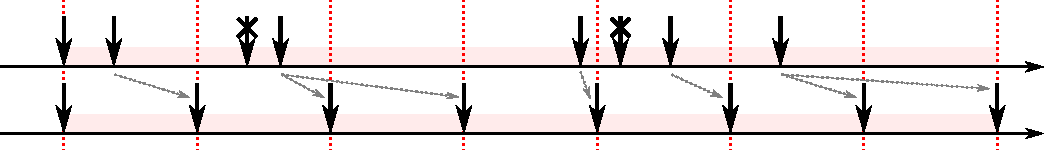
\includegraphics[width=12cm]{fig/rate_control_tt.pdf}
    \CaptionFigSpace
    \caption{An example of the behaviour of a temporal firewall where the upper timeline represents the arrival instances of \glspl*{msg} and the lower timeline represents the release instances of \glspl*{msg}.}
    \label{fig_rate_ctl_tt}
\BotFigSpace
\end{center}\end{figure}
%------------------------------------------------------------------
An example of a behaviour of a temporal firewall is illustrated in \Fig{\ref{fig_rate_ctl_tt}}.
The upper time line represents the arrival instances of \glspl*{msg} at the input of a temporal firewall and the lower timeline represents the release instances of \glspl*{msg} from the output of the temporal firewall.
The vertical dotted lines indicate the rate of the clock that triggers the temporal firewall.
A crossed-out arrow represents a \gls*{msg} that is overwritten by a newer \gls*{msg} (\eg the third \gls*{msg} is overwritten by the fourth and the sixth \gls*{msg} is overwritten by the seventh).

Multiple temporal firewalls can be synchronized by synchronizing the clock signals triggering the temporal firewall.
This is only possible if the clock rate of the synchronized temporal firewalls is equal.
% A set of synchronized temporal firewalls satisfies \Propty{\ref{propty_tf_out}} and \Propty{\ref{propty_tf_in}}:
% \begin{property}[Temporal Firewall Output]
%     \label{propty_tf_out}
%     At the start of a round $r$, each temporal firewall produces exactly one \gls*{msg}.
% \end{property}
% \begin{property}[Temporal Firewall Input]
%     \label{propty_tf_in}
%     Before the start of the next round $r+1$, each temporal firewall consumes exactly one \gls*{msg}.
% \end{property}
% These properties are ensured by the fact that all input and output ports of temporal firewalls are decoupled and that a temporal firewall is periodically triggered by the connected clock signal.

%------------------------------------------------------------------
\begin{figure}[bht]\begin{center}
\TopFigSpace
    \centering
    \includegraphics[width=9cm]{fig/sia_firewall_dec.pdf}
    \CaptionFigSpace
    \caption{A temporal firewall with a decoupled port pair $\langle a_{in}, a_{out} \rangle$ and a port $p_{clk}$ which is connected to a clock signal.}
    \label{fig_tcm_tfw}
\BotFigSpace
\end{center}\end{figure}
%------------------------------------------------------------------

A temporal firewall $N_{\mathit{FW}}$ with its corresponding \gls{sia} $\descSIA{N}_{\mathit{FW}}$ is depicted in \Fig{\ref{fig_tcm_tfw}}.
The ports $a_{in}$ and $a_{out}$ are decoupled in synchronisation.
A clock signal is connected to the port $p_{clk}$.
For simplicity I will use the notation \channel{tf,->}{$a(p_{clk})$} to describe a temporal firewall on channel $a$, triggered by the clock signal $p_{clk}$, as depicted in \Fig{\ref{fig_tcm_tfw}}.
Note that decoupled \gls{fifo} channels of length one instead of synchronous channels are connected to the input and output port of a temporal firewall.
% Note that the symbol for a temporal firewall (\channel{tf,->}{$a(p_{clk})$}) and the channel connected to the input and the output of the temporal firewall is represented by a double-lined arrow.
This is because of the following:
While the input and output of a temporal firewall is decoupled in synchronisation by default, the output of the producing process and the input of the consuming process, connected to the temporal firewall, must not necessarily be decoupled in synchronisation.
In order to achieve this separate control of decoupling in synchronisation, decoupling in time is required, hence, buffered channels are used by default.

By connecting all input and output ports of a \gls{pnsc} (or a single process) to synchronized temporal firewalls, a time-triggered behaviour is imposed onto the \gls{pnsc}.
I call such a \gls{pnsc} a time-triggered \gls{pnsc}.
The time-triggered behaviour is enforced because \glspl*{msg} can only reach the time-triggered \gls{pnsc} through temporal firewalls and the temporal firewalls produce \glspl*{msg} at the specified rate which causes the time-triggered \gls{pnsc} to trigger at the specified rate.
Temporal firewalls can be connected to a single process or a \gls{pnsc}.
When connected to a single process, no sporadic triggering is possible because the time-triggered process is completely decoupled from the rest of the network through temporal firewalls.
The \gls{wcet} of the process must be guaranteed to be smaller than the triggering rate imposed by the temporal firewalls.
When connected to a \gls{pnsc}, only processes that communicate with the environment of the time-triggered \gls{pnsc} are decoupled by temporal firewalls.
Other processes inside the time-triggered \gls{pnsc} may still be triggered through sporadic \gls*{msg} transmissions.

%------------------------------------------------------------------
\begin{figure}[bht]\begin{center}
\TopFigSpace
    \centering
    \includegraphics[width=10cm]{fig/procs_tf.pdf}
    \CaptionFigSpace
    \caption{An example of a time-triggered \gls{pnsc} where the \gls{pnsc} is decoupled through temporal firewalls while processes inside the time-triggered \gls{pnsc} trigger sporadically (\eg process $P_2$).}
    \label{fig_tcm_tfnw}
\BotFigSpace
\end{center}\end{figure}
%------------------------------------------------------------------
As an example let's consider the time-triggered \gls{pnsc} depicted in \Fig{\ref{fig_tcm_tfnw}}.
The process $P_1$ interacts through the temporal firewalls $a_1(p_{clk})$ and $a_2(p_{clk})$ with its environment to the left and process $P_3$ interacts through $a_5(p_{clk})$ and $a_6(p_{clk})$ with its environment to the right.
Consequently, the time-triggered \gls{pnsc}, framed by the four temporal firewalls $a_1$, $a_2$, $a_5$, and $a_6$, is decoupled from its environment through the temporal firewalls.
Process $P_2$, however, which is placed inside the time-triggered \gls{pnsc} is not connected to any temporal firewall and is triggering sporadically depending on the arrival of \glspl*{msg} from process $P_1$.
Process $P_3$ is triggered through \glspl*{msg} arriving at the input $a_6$, produced at a rate $p_{clk}$ from a temporal firewall, and through \glspl*{msg} arriving through input port $a_4$, sporadically produced by process $P_2$.
A time-triggered \gls{pnsc} $\mathit{PN}$, framed by synchronized temporal firewalls, must satisfy \Propty{\ref{propty_tt_in}} and \Propty{\ref{propty_tt_out}}.
\begin{property}[Time-triggered Input]
    \label{propty_tt_in}
    At the start of each round $r$, a process $P \in \mathit{PN}$ connected to a temporal firewall via an input port consumes at least one \gls*{msg}.
\end{property}
\begin{property}[Time-triggered Output]
    \label{propty_tt_out}
    Before the start of the next round $r+1$, a process $P \in \mathit{PN}$ connected to a temporal firewall via an output port produces at least one \gls*{msg}.
\end{property}
Note that if more than one \gls*{msg} is consumed or produced by a process $P \in \mathit{PN}$, connected to a temporal firewall, the corresponding port of the process must be decoupled in order to not block the process, given that a temporal firewall produces and consumes exactly one \gls*{msg}.

To tighten the control on the rate of \glspl*{msg} passing in the time-triggered \gls{pnsc} $\mathit{PN}$, each process $P \in \mathit{PN}$ must be framed by synchronized temporal firewalls.
This is illustrated in \Fig{\ref{fig_tcm_ttnw}} which depicts the same example as \Fig{\ref{fig_tcm_tfnw}} but without any sporadic triggering of processes.
%------------------------------------------------------------------
\begin{figure}[bht]\begin{center}
\TopFigSpace
    \centering
    \includegraphics[width=11cm]{fig/procs_tt.pdf}
    \CaptionFigSpace
    \caption{An example of a time-triggered \gls{pnsc} where each process in the \gls{pnsc} is decoupled through temporal firewalls.}
    \label{fig_tcm_ttnw}
\BotFigSpace
\end{center}\end{figure}
%------------------------------------------------------------------
Here, in each clock cycle \glspl*{msg} are passed from one process to the next via temporal firewalls and no sporadic triggering is occurring in the time-triggered \gls{pnsc}.
However, this is only the case if temporal firewalls are synchronized which allows a concatenation of two temporal firewalls, triggered by the same clock rate, to be merged into one (as depicted in \Fig{\ref{fig_tcm_ttnw}}).

If the temporal firewalls, framing the processes are not synchronized, \ie their clock rate differs, temporal firewalls cannot be merged and the time instant of when one temporal firewall produces a \gls*{msg} is not necessarily synchronized with the time instant the neighbouring temporal firewall is consuming a \gls*{msg}.
Consequently, the time instance of passing a message from one process to another is not coordinated.
An example of such a case is depicted in \Fig{\ref{fig_tcm_ttnw_async}} where the processes $P_1$ and $P_2$ are framed by temporal firewalls, each triggered by a different clock rate $clk_1$ and $clk_2$, respectively.
%------------------------------------------------------------------
\begin{figure}[bht]\begin{center}
\TopFigSpace
    \centering
    \includegraphics[width=9cm]{fig/procs_tt_async.pdf}
    \CaptionFigSpace
    \caption{An example of a time-triggered \gls{pnsc} where each process in the \gls{pnsc} is decoupled through a temporal firewall with a different clock rate each.}
    \label{fig_tcm_ttnw_async}
\BotFigSpace
\end{center}\end{figure}
%------------------------------------------------------------------

%------------------------------------------------------------------------------
\subsection{Rate-bounded Communication}
\label{sect_cci_decoupling_rate}
To control the bandwidth usage of a communication channel I introduce the concept of rate-bounded communication.
The idea is to introduce a timed guard on a communication channel in order to limit the production rate of \glspl*{msg} in the channel to a specified upper bound.
This bound is specified by the consumer process.
This allows a better prediction of the maximum communication bandwidth demand.
A time interval, called \emph{inter-arrival time}, is used to measure and control the communication rate.
The inter-arrival time describes the elapsed time between the arrival of two consecutive \glspl*{msg}.
If the inter-arrival time of a \gls*{msg} is lower than a specified bound, an action is performed to either delay the \gls*{msg} or to discard it.
Rate-bounded communication is orthogonal to communication coupling and can be applied on all types of coupling configurations of two interacting processes.
However, depending on whether the output of a producer process is decoupled in synchronisation or not, a different method is used to achieve rate-bounded communication.

If the output of the producer process is coupled in synchronisation, \ie the write access to the channel is blocking, back-pressure is used to achieve rate-bounded communication:
The write access not only blocks on write operations if the communication partner is not ready but also if the inter-arrival time of \glspl*{msg} is lower than a specified bound.
% If the output of the producer process is not decoupled, \ie the input-port of the connected \gls{fifo} buffer is not decoupled (\Fig{\ref{fig_sia_fifo}} or \Fig{\ref{fig_sia_cci_out}}), back-pressure is used to achieve rate-bounded communication.
% Hence, the \gls{fifo} buffer not only blocks on write operations if the buffer is full but also if the inter-arrival time of \glspl*{msg} is lower than a specified bound.
Due to the blocking semantics of this rate-control the producing process is not only influenced by the rate of the consuming process but also by the imposed rate-bound on the communication channel.
Let $t_{mia}(p_i)$ describe the minimal inter-arrival time specified on an input port $p_i \in \mathcal{P}^I(N)$ of a process $N$ then the maximum rate $r_{max}(p_i)$ of arriving \glspl*{msg} on port $p_i$ is defined in \Equ{\ref{eq_rate_max}}.
\begin{equation}
    \label{eq_rate_max}
    r_{max}(p_i) = \frac{1}{t_{mia}(p_i)}
\end{equation}
I use the notation \channel{dashed,->}{$p_i(t_{mia})$} to describe a channel $p_i$ bound by the rate $r_{max}(p_i)$ as defined in \Equ{\ref{eq_rate_max}}.

If, on the other hand, the output port of the producer is decoupled in synchronisation, \ie the write access to the channel is non-blocking, discarding of \glspl*{msg} is used to limit the communication rate.
Hence, in addition to discarding \glspl*{msg} if the communication partner is not ready, the corresponding channel also discards \glspl*{msg} if the communication rate is exceeded.
% If, on the other hand, the output port of the producer is decoupled, \ie the input-port of the connected \gls{fifo} buffer is decoupled (\Fig{\ref{fig_sia_cci_in}} or \Fig{\ref{fig_sia_cci_bi}}), discarding of \glspl*{msg} is used to limit the communication rate.
% Hence, in addition to discarding \glspl*{msg} if the buffer is full, the corresponding \gls{fifo} buffer also discards \glspl*{msg} if the communication rate is exceeded.
Due to the discarding of \glspl*{msg} the rate-bound on the communication channel does not impose back-pressure onto the producer process.

In the following I will propose two types of protocols that enforce rate-control without interfering with the producer by discarding \glspl*{msg}:
\begin{enumerate}
    \item The \emph{\gls{mirt}} protocol guarantees that the communication rate at a port $p_i$ never exceeds the maximum rate $r_{max}(p_i)$ as defined in \Equ{\ref{eq_rate_max}}.
        This is ensured by enforcing a minimal time of $t_{mia}$ between the release of two consecutive \glspl*{msg}.
    \item The \emph{\gls{pbrt}} protocol allows to release at maximum one \gls*{msg} per period $t_{max}(p_i)$ at a port $p_i$ but does not enforce a minimal time between two consecutive \glspl*{msg}.
        This allows small peak loads where the time between two consecutive \glspl*{msg} releases is smaller than $t_{mia}$ but ensures that on average the rate of $\frac{1}{t_{mia}(p_i)}$ is not exceeded.
\end{enumerate}

Both types of protocols can either employ a buffer, \ie decouple the communication in time, in order to delay messages and reduce the number of discarded \glspl*{msg} or use a more aggressive strategy and discard \glspl*{msg} straight away if they do not respect the imposed timed guard.
A buffered guard must be an active process because it must be able to release a \gls*{msg} at a later time without blocking the producer process.
Also, a buffered guard increases the latency of a single \gls*{msg} due to the imposed delay.
An unbuffered guard is much simpler because \glspl*{msg} must not be delayed but only discarded if the minimal inter-arrival time is not respected.
This leads to more losses of \glspl*{msg} but the latency of a single \gls*{msg} is not changed.

In the following subsection I will describe each protocol in more detail and give examples.
I use the following notations to identify time values associated to guards:
\begin{description}
    \item[$t_{a}(m)$]
        denotes the arrival time of a \gls*{msg} $m$ at the guard.
    \item[$t_r(m)$]
        denotes the time of the release of a \gls*{msg} $m$ from the guard to its connected \gls{fifo} buffer.\\
        If a \gls*{msg} $m$ is discarded $t_r(m) = \infty$.\\
        For the initial \gls*{msg} $m_0$ I define $t_r(m_0) = t_a(m_0)$.
    \item[$t_{nr}(m)$]
        denotes the minimum time to the next release after the arrival of a \gls*{msg} $m$ at the guard.\\
        For the initial \gls*{msg} $m_0$ I define $t_{nr}(m_0) = t_r(m_0) + t_{mia}$.
    \item[$t_{mia}$]
        denotes the minimum inter-arrival time of two consecutive \glspl*{msg}.
\end{description}

\subsubsection{Rate-control with the MIRT protocol}
The \gls{mirt} protocol accepts \glspl*{msg} only if the minimal inter-arrival time is respected.
Once a \gls*{msg} arrives at the guard, all consecutive \glspl*{msg} arriving within the minimal inter-arrival time interval are discarded.
If the minimal inter-arrival time is respected, \glspl*{msg} are released immediately.
Let $( m_{i-1}, m_i )$ be a sequence of \glspl*{msg} arriving at the guard, then the release time $t_r(m_i)$ of \gls*{msg} $m_i$ is defined in \Equ{\ref{eq_mirt_release}}
\begin{equation}
    t_r(m_i) =
        \begin{cases}
            t_a(m_i) & \quad \text{if } t_a(m_i) \geq t_{nr}(m_{i-1})\\
            \infty   & \quad \text{otherwise}\\
        \end{cases}
    \label{eq_mirt_release}
\end{equation}
and the minimum time of the next release $t_{nr}(m_i)$ after the arrival of \gls*{msg} $m_i$ is defined in \Equ{\ref{eq_mirt_next_release}}
\begin{equation}
    t_{nr}(m_i) =
        \begin{cases}
            t_r(m_i) + t_{mia} & \quad \text{if } t_r(m_i) < \infty\\
            t_r(m_{i-1})       & \quad \text{otherwise}\\
        \end{cases}
    \label{eq_mirt_next_release}
\end{equation}

This is illustrated in the example depicted in \Fig{\ref{fig_rate_ctl_mirt}}.
The arrows on the upper time-line depict the arrival times of the \glspl*{msg}.
Crossed-out arrows represent \glspl*{msg} that are discarded.
The minimal inter-arrival time interval is represented as the lightly coloured area, framed by two dotted lines.
The arrows on the lower time-line represent the release times of \glspl*{msg}.
The timer is activated upon releasing a \gls*{msg} as depicted by the dotted lines in \Fig{\ref{fig_rate_ctl_mirt}}.

\subsubsection{Rate-control with the buffered MIRT protocol}
The buffered \gls{mirt} protocol buffers an arriving \gls*{msg} to delay its progress.
Once the specified minimal inter-arrival time is respected, the delayed \gls*{msg} is released.
\Glspl*{msg} are discarded if multiple \glspl*{msg} arrive within one minimal inter-arrival time interval.
Let $( m_{i-1}, m_i, m_{i+1} )$ be a sequence of \glspl*{msg} arriving at the guard, then the release time $t_r(m_i)$ of \gls*{msg} $m_i$ is defined in \Equ{\ref{eq_bmirt_release}}
\begin{equation}
    t_r(m_i) =
        \begin{cases}
            t_a(m_i)        & \quad \text{if } t_a(m_i) \geq t_{nr}(m_{i-1})\\
            t_{nr}(m_{i-1}) & \quad \text{if } t_a(m_{i+1}) \geq t_{nr}(m_{i-1})\\
            \infty          & \quad \text{otherwise }\\
        \end{cases}
    \label{eq_bmirt_release}
\end{equation}
The minimum time of the next release $t_{nr}(m_i)$ after the arrival of \gls*{msg} $m_i$ is equivalent to the unbuffered \gls{mirt} protocol as defined in \Equ{\ref{eq_mirt_next_release}}.

\Fig{\ref{fig_rate_ctl_bmirt}} represents an example where the same \gls*{msg} arrival times are used as in the previous example but here, a buffered version of the \gls{mirt} protocol is used to release the \glspl*{msg}.
As a consequence, fewer \glspl*{msg} are discarded at the cost of increasing the latency of individual \glspl*{msg}.
If multiple \glspl*{msg} arrive within a minimal inter-arrival time interval, the newest \gls*{msg} is kept and the older ones are discarded (\eg in \Fig{\ref{fig_rate_ctl_bmirt}} the fourth \gls*{msg} replaces the third one and the seventh \gls*{msg} replaces the sixth one).
This lies in contrast to the unbuffered \gls{mirt} protocol where the newer \glspl*{msg} are discarded (see \Fig{\ref{fig_rate_ctl_mirt}}).
This difference is solely due to the presence of the buffer which allows to store the newer message which is not possible in the unbuffered case.
As with the unbuffered \gls{mirt} protocol, also here a timer is activated upon release of a \gls*{msg}.

\subsubsection{Rate-control with the PBRT protocol}
The \gls{pbrt} protocol is based on a periodic timer with period $t_{mia}$.
The policy is to allow the release of at maximum one \gls*{msg} per period.
This ensures that an average rate of $\frac{1}{t_{mia}}$ is not exceeded.
However, it does not specify a maximal rate and allows bursts during a short period, \ie the time between two consecutive \glspl*{msg} can be smaller that the specified period but the average rate can never be exceeded.
Let $( m_{i-1}, m_i )$ be a sequence of \glspl*{msg} arriving at the guard, then the release time $t_r(m_i)$ of \gls*{msg} $m_i$ is equivalent to the unbuffered \gls{mirt} protocol as defined in \Equ{\ref{eq_mirt_release}}.
The minimum time of the next release $t_{nr}(m_i)$ after the arrival of \gls*{msg} $m_i$ is defined in \Equ{\ref{eq_pbrt_next_release}}
\begin{equation}
    t_{nr}(m_i) = (k+1) t_{mia} \text{ with } k \in \mathbb{Z} \ . \ kt_{mia} \leq t_r(m_i) < (k+1)t_{mia}
    \label{eq_pbrt_next_release}
\end{equation}

\Fig{\ref{fig_rate_ctl_pbrt}} depicts an example of a sequence of \glspl*{msg}, released according to the \gls{pbrt} protocol.
Again, the same arrival times of \glspl*{msg} as in the previous examples are used.
In contrast to the \gls{mirt} protocol, the timer is activated periodically, as depicted by the dotted lines.
During a short time the minimal inter-arrival time is violated to compensate for a short burst of \glspl*{msg}.
This allows to reduce the number of discarded \glspl*{msg}.
The violation of the minimal inter-arrival time is highlighted in \Fig{\ref{fig_rate_ctl_pbrt}}.

\subsubsection{Rate-control with the buffered PBRT protocol}
The buffered \gls{pbrt} protocol reduces the number of discarded \glspl*{msg} by using a buffer to delay \glspl*{msg} in order to satisfy the rate requirements.
As with the unbuffered \gls{pbrt} protocol, the timer is periodic with period $t_{mia}$.
An arriving \gls*{msg} can still be discarded if the buffer is already used to delay a \gls*{msg} that arrived before.
In this case the new \gls*{msg} overwrites the old one in the buffer.
Let $( m_{i-1}, m_i, m_{i+1} )$ be a sequence of \glspl*{msg} arriving at the guard, then the release time $t_r(m_i)$ of \gls*{msg} $m_i$ is equivalent to the buffered \gls{mirt} protocol defined in \Equ{\ref{eq_bmirt_release}}.
The minimum time of the next release $t_{nr}(m_i)$ after the arrival of \gls*{msg} $m_i$ is equivalent to the unbuffered \gls{pbrt} protocol as defined in \Equ{\ref{eq_pbrt_next_release}}.

An example of the buffered \gls{pbrt} protocol, applied on a sequence of \glspl*{msg} is depicted in \Fig{\ref{fig_rate_ctl_bpbrt}}.
Also here, the arrival times of the \glspl*{msg} are the same as in the previous examples to allow a comparison between the different approaches.
With this protocol only one \gls*{msg} is discarded.
Again, in contrast to the unbuffered version, the newer \gls*{msg} overwrites the older one and, consequently, the older one is discarded.
This comes at the cost of increasing the latency of individual \glspl*{msg} and allowing a violation of the minimal inter-arrival time.
In \Fig{\ref{fig_rate_ctl_bpbrt}}, the interval where a burst of \glspl*{msg} is accepted is highlighted.

%------------------------------------------------------------------
\begin{figure}[bht]
    \TopFigSpace
    \centering
    \begin{subfigure}[h]{\linewidth}
        \centering
        \includegraphics[width=12cm]{fig/rate_control_mirt.pdf}
        \CaptionFigSpace
        \caption{An example of rate-control with the unbuffered \gls{mirt} protocol.}
        \label{fig_rate_ctl_mirt}
        \vspace{1em}
    \end{subfigure}
    \begin{subfigure}[h]{\linewidth}
        \centering
        \includegraphics[width=12cm]{fig/rate_control_bmirt.pdf}
        \CaptionFigSpace
        \caption{An example of rate-control with the buffered \gls{mirt} protocol.}
        \label{fig_rate_ctl_bmirt}
        \vspace{1em}
    \end{subfigure}
    \begin{subfigure}[h]{\linewidth}
        \centering
        \includegraphics[width=12cm]{fig/rate_control_pbrt.pdf}
        \CaptionFigSpace
        \caption{An example of rate-control with the unbuffered \gls{pbrt} protocol.}
        \label{fig_rate_ctl_pbrt}
        \vspace{1em}
    \end{subfigure}
    \begin{subfigure}[h]{\linewidth}
        \centering
        \includegraphics[width=12cm]{fig/rate_control_bpbrt.pdf}
        \CaptionFigSpace
        \caption{An example of rate-control with the buffered \gls{pbrt} protocol.}
        \label{fig_rate_ctl_bpbrt}
    \end{subfigure}
\caption{Examples of rate-control protocols.
In each figure the upper time-line represents the arrival instances of \glspl*{msg} while the lower time-line represents the release instances of \glspl*{msg}.}
    \label{fig_rate_ctl}
    \BotFigSpace
\end{figure}
%------------------------------------------------------------------

%==============================================================================
\section{Message Semantics}
\label{sect_tcm_msg}
In \glspl{pnsc}, communication decoupling in synchronization, as described in \Sect{\ref{sect_cci_decoupling_sync}}, can lead to loss or duplication of \glspl*{msg}.
Depending on the content the \gls*{msg} carries, this can be more or less problematic.
The level of criticality of the transmitted information is an aspect that dictates whether loss or duplication of the information is problematic.
For example, \glspl*{msg} that carry information to perform a monetary transaction have a high criticality and must not be lost.
The loss of a signal of a TV remote control, on the other hand, is inconvenient at most as it can simply be repeated until the transmission is successful.

Apart from the criticality, also the type of the transmitted information plays a crucial role and can alleviate the criticality due to an inherent resilience.
Traditionally, one distinguishes between message types where the content can have information of how to update a subsystem (aka event message) or information about the state of a subsystem (aka state message).
As Kopetz~\cite{kopetz2011d} points out, state messages are well suited for time-triggered systems and event messages for sporadic (event-triggered) systems.
However, as Powell~\cite{powell2002} points out, it is not necessary that a time-triggered system operates solely with state messages nor is it necessary for a sporadic system to operate with event messages.
In the following I will define each message type with respect to message loss and duplication and provide typical application examples for different message types.
I further propose a novel message type, called semi-state message, that has some properties from state messages and some from event messages.
I define a semi-state message in \Def{\ref{def_semi_state_msg}}, a state message in \Def{\ref{def_state_msg}}, and an event message in \Def{\ref{def_event_msg}}.

\begin{definition}[Semi-state Message]
\label{def_semi_state_msg}
A message in a system is called a {\em semi-state message} if it enables a correct system state after a previous message of the same type has been lost and the repeated processing of a single message is tolerated by the system.
\end{definition}

\begin{definition}[State Message]
\label{def_state_msg}
A message in a system is called a {\em state message} if it is a {\em semi-state message} and its arrival makes the processing of non-processed previous messages of the same type obsolete.
\end{definition}

\begin{definition}[Event Message]
\label{def_event_msg}
Every message in a system that is not a semi-state message (and consequently also not a state message) is an {\em event message}.
In case it is not known whether a message is an event or (semi-) state message, it is safe to assume it to be an {\em event message}.
\end{definition}

The loss or duplication of a \gls*{msg} is tolerated by a system if the \gls*{msg} is either of type state message or semi-state message.
In a state message based communication scheme, the producer observes the value of the state variable at a particular time instant and transmits a state message.
An observation is expressed by the triple $<name_{obseravtion}, value, t_{observation}>$.
The transmitted information is useful on its own and no knowledge of a previous transmission is required by the consumer.
A consumer of state messages is only interested in the newest state information of the sender.
Hence, a state message already residing in the communication buffer can be overwritten by a new message without losing any information.
Also, messages can be duplicated without problem as a consumer can perform a non-destructive read to keep the information available for possible further reading operations before a new state message arrives (read access is decoupled in space, time, and synchronisation).
These properties make state messages useful for fault tolerant systems and hence for safety-critical systems.
% Due to this property, message losses and erroneous transmissions may cause bad behaviour only as long as no new correct message is received by the consumer.

In the case of a semi-state message, while the loss or duplication of a \gls*{msg} is tolerated, it is not desirable because the quality of the service might degrade.
Hence, a semi-state message has similar properties as a state message but a system benefits from keeping a history of non-consumed \glspl*{msg}, \ie a \gls*{msg} is not made obsolete with the arrival of a newer \gls*{msg}.

There are cases when (semi-)state messages can not be used or only at high costs.
If, for example, the state variable of the producer is not easily observable or needs to be accessed concurrently (\eg concurrent bank transactions), an infrastructure must be put in place that allows concurrent access.
A message is classified as event message, if the properties of a (semi-)state message, as defined above, are not sufficient to ensure a correct behaviour.
In an event message based communication scheme, an event causes the state variable to change its value.
The producer then transmits the change from the old to the new state variable that was caused by the event.
An event can be expressed by the triple $<name_{event}, \Delta value, t_{event}>$.
% The state variable of the producer can be reconstructed in the consumer by accumulating all event messages.
Generally, it is important that no event message is lost or duplicated and that the order of the messages is preserved.
Event message semantics preserves event safety, \ie prevents losses and duplication of \glspl*{msg}, and is the default assumption of a communication channel, as defined in \Def{\ref{def_channel_msg_semantics}}.
\begin{definition}[Message Semantics of Communication Channel]
\label{def_channel_msg_semantics}
A communication channel that carries only {\em state messages} has a state-message semantics.
A communication channel that carries only {\em state messages} and {\em semi-state messages} has a semi-state-message semantics.
A communication channel that carries {\em event messages} has an event-message semantics.
\end{definition}

It is a design decision of whether the message semantics of a communication channel can be explicitly declared to be of (semi-) state message semantics.
Having a state message or a semi-state message semantics typically depends on the application context.
For example, the stream of video frames of a surveillance camera does have \emph{state semantics} if only life view is required:
Only the most recent picture is relevant but it is important that the most recent picture reflects the current situation of the real world.
But the same video stream would have \emph{semi-state semantics} if it is provided as an online stream that can be consumed over great distances and lossy channels, \ie a good trade-off between a minimum acceptable loss of frames and a minimum acceptable transmission delay is required.
However, if the video is recorded and a later frame-by-frame analysis is required then the video stream would have \emph{event semantics}.

%==============================================================================
\section{Cross-criticality Interfaces}
\label{sect_tcm_cci}
When interconnecting processes with different criticality levels it is important to provide suitable interfaces that allow communication without interference from processes with a lower criticality level towards processes with a higher criticality level.
Further, such interfaces must allow the coexistence of processes with different timing behaviours and message semantics.
I call such interfaces \gls{cci} because they allow interaction between processes of different criticality levels.

Throughout this chapter I introduced communication mechanisms that allow to decouple interactions of processes in space, time, and synchronisation and proposed communication channels that allow to control the communication and execution rate of processes.
In the following list I provide an overview of the different communication channels introduced throughout this chapter and propose new composed channels where multiple properties are combined.
Only combinations are listed that have sensible semantics and a potential use in real applications:
\begin{description}
    \item[\channel{->}{$a$}] depicts a synchronous channel $a$.
        Decoupling of such a channel is not practical (see \Sect{\ref{sect_cci_decoupling_sync}}).
    \item[\channel{double,->}{$a[l]$}] depicts a \gls{fifo} channel $a$ of length $l$.
        Such a channel can be decoupled in synchronisation on its input \channel{double,)->}{$a[l]$}, its output \channel{double,->>}{$a[l]$}, or both \channel{double,)->>}{$a[l]$}.
    \item[\channel{dashed, ->}{$a(t)$}] depicts a synchronous channel $a$ that is bound by a rate defined by $t$.
        Decoupling of such a channel is not practical (see \Sect{\ref{sect_cci_decoupling_sync}}).
    \item[\channel{double,dashed,->}{$a(t)[l]$}] depicts a \gls{fifo} channel $a$ of length $l$ that is bound by a rate defined by $t$.
        Such a channel can be decoupled in synchronisation on its input \channel{double,dashed,)->}{$a(t)[l]$}, its output \channel{double,dashed,->>}{$a(t)[l]$}, or both \channel{double,dashed,)->>}{$a(t)[l]$}.
    \item[\channel{tf,->}{$a(clk)$}] depicts a channel $a$ with an incorporated temporal firewall that is triggered at a rate $clk$.
        Such a channel can be decoupled in synchronisation on its input \channel{tf,)->}{$a(clk)$}, its output \channel{tf,->>}{$a(clk)$}, or both \channel{tf,)->>}{$a(clk)$}.
\end{description}

Table \ref{tab_pattern} lists the same communication channels and provides an overview of properties of each channel.
% The row \emph{channel} lists the different communication channels with their corresponding symbol.
The following properties are described:
\begin{description}
    \item[write] indicates whether the write access to the channel is blocking (block) or non-blocking ($\neg$block), \ie whether the write access is coupled or decoupled in synchronisation.
    \item[read] indicates whether the read access to the channel is blocking (block) or non-blocking ($\neg$block), \ie whether the read access is coupled or decoupled in synchronisation.
    \item[lossy] indicates whether \glspl*{msg} can potentially be lost (yes) or not (no).
    \item[copy] indicates whether \glspl*{msg} can potentially be duplicated (yes) or not (no).
    \item[rate] describes the communication rate of transmitted \glspl*{msg}.
    \item[buffer] indicates whether the channel is buffered (yes) or unbuffered (no), \ie whether the channel is decoupled or coupled in time.
    \item[event] indicates if the channel supports event messages (yes) or if (semi-)state messages are better suited (no).
\end{description}

The table shows that imposing a fixed communication rate with a temporal firewall, as described in \Sect{\ref{sect_tcm_time_tt}}, is only suitable for (semi-)state messages because loss or duplication of \glspl*{msg} can happen independently of communication coupling.
The decision of whether a read or write access on a temporal firewall should be blocking or non-blocking depends solely on the intended progression control of the process:
It might be desirable to block a producer process, connected to a temporal firewall, until the produced \gls*{msg} is consumed by the temporal firewall in order to avoid unnecessary computation efforts of the producer process.
On the other hand it might be desirable to allow the producer process to refine its result and overwrite the previous output.
The latter requires decoupling in synchronisation to make the write access to the channel non-blocking.

%------------------------------------------------------------------
\begin{table}[bht]
    \renewcommand{\arraystretch}{1.3}
    \TopTabSpace
    \caption{A list of the properties of communication channels, formed from different combinations of communication patterns.}
    \label{tab_pattern}
    \CaptionTabSpace
    \centering
    % \normalsize
    % \small
    \begin{tabular}{c|*{7}{|c}}
                                  & write       & read        & lossy & copy & rate     & buffer & event \\
        \hline
        \hline
        \channel{->}{}            & block       & block       & no    & no   & sporadic & no     & yes   \\
        \hline
        \channel{fifo, ->}{}      & block       & block       & no    & no   & sporadic & yes    & yes   \\
        \channel{fifo, ->>}{}     & block       & $\neg$block & no    & yes  & sporadic & yes    & no    \\
        \channel{fifo, )->}{}     & $\neg$block & block       & yes   & no   & sporadic & yes    & no    \\
        \channel{fifo, )->>}{}    & $\neg$block & $\neg$block & yes   & yes  & sporadic & yes    & no    \\
        \hline
        \channel{tb, ->}{}        & block       & block       & no    & no   & bounded  & no     & yes   \\
        \hline
        \channel{tb,fifo, ->}{}   & block       & block       & no    & no   & bounded  & yes    & yes   \\
        \channel{tb,fifo, ->>}{}  & block       & $\neg$block & no    & yes  & bounded  & yes    & no    \\
        \channel{tb,fifo, )->}{}  & $\neg$block & block       & yes   & no   & bounded  & yes    & no    \\
        \channel{tb,fifo, )->>}{} & $\neg$block & $\neg$block & yes   & yes  & bounded  & yes    & no    \\
        \hline
        \channel{tf,->}{}         & block       & block       & yes   & yes  & fixed    & yes    & no    \\
        \channel{tf,->>}{}        & block       & $\neg$block & yes   & yes  & fixed    & yes    & no    \\
        \channel{tf,)->}{}        & $\neg$block & block       & yes   & yes  & fixed    & yes    & no    \\
        \channel{tf,)->>}{}       & $\neg$block & $\neg$block & yes   & yes  & fixed    & yes    & no    \\
    \end{tabular}
    \BotTabSpace
\end{table}
%------------------------------------------------------------------

The attributes of \emph{sporadic} communication channels are equivalent to the attributes of channels with a \emph{bounded} communication rate when considering the same coupling configuration (with the exception of the \emph{rate} attribute).
This means that bounding the communication rate, as described in \Sect{\ref{sect_cci_decoupling_rate}}, only influences the communication rate but does not change the communication coupling behaviour of a channel.

%------------------------------------------------------------------------------
\subsection{Mixed-criticality Network with CCIs}
\label{sect_tcm_cci_example}
In this section I describe a mixed-criticality video processing application that relies on different communication channels, introduced in this chapter.
The basic principle of the application is to record video images with a camera, perform two independent video processing tasks on the video frames, and display the result on a screen.
One of the two video processing tasks is of high criticality and must be guaranteed to perform correctly while the other step is of low criticality as it only improves the result but is not absolutely necessary.
The challenge of this application is that the lower critical processing task is more complicated and requires more resources than the high criticality task and it must be ensured that the low criticality task does not interfere with the high criticality task.

The example depicted in Figure \ref{fig_mc_pnsc_ex} shows a \gls{pnsc} that models such an image processing application.
The process $P_{cam}$ produces \glspl*{msg} containing video frames and communicates them to the process $P_{copy}$.
The process $P_{copy}$ copies the arriving \glspl*{msg} to each of two connected channels at its output ports.
The upper channel connects to the process $P_{filter}$ where the video frames, consumed via its input port, are processed and then sent to the output port.
The lower channel connects to the process $P_{fd}$ where a complex feature detection algorithm is executed on the video frames.
The process $P_{merge}$ consumes \glspl*{msg} from the processes $P_{filter}$ and $P_{fd}$ and merges the two video frames into one.
\Glspl*{msg} with the merged video frames are then transmitted to the process $P_{screen}$ where the video is displayed.
%------------------------------------------------------------------
\begin{figure}[bht]\begin{center}
\TopFigSpace
    \centering
    \includegraphics[width=\linewidth]{fig/mc_pnsc_ex.pdf}
    \CaptionFigSpace
    \caption{An example of a mixed-criticality video processing application where ports are decoupled in synchronisation to prevent interference from the low critical process $P_{fd}$ towards the high criticality process $P_{filter}$.}
    \label{fig_mc_pnsc_ex}
\BotFigSpace
\end{center}\end{figure}
%------------------------------------------------------------------

All communication channels are buffered to allow a variation in the production rate of the processes.
The channel $cam$, connecting process $P_{cam}$ with process $P_{copy}$, is bounded to a maximum rate of $\frac{1}{24}$ which is sufficient for this particular video processing application.
% Back-pressure limits the production rate of the producing processes while \gls{fifo} buffers allow a variation of the production rate.
The process $P_{filter}$ is of high criticality (the box with the thick border in \Fig{\ref{fig_mc_pnsc_ex}}) and process $P_{fd}$ is of low criticality, hence, it must be ensured that $P_{fd}$ is not interfering with $P_{filter}$.
To achieve this, first, the output $f_2$ of process $P_{copy}$ is decoupled in synchronisation to prevent back-pressure from the low-criticality process $P_{fd}$.
Consequently, process $P_{copy}$ cannot be blocked by process $P_{fd}$ which prevents indirect interference from process $P_{fd}$ towards process $P_{filter}$.
Second, the input $fd$ of process $P_{merge}$ is decoupled in synchronisation to prevent a blocking read access from process $P_{merge}$ to this channel which prevents any indirect interference from process $P_{fd}$ towards process $P_{filter}$ via process $P_{merge}$.

Additionally, the channel $f_2$ is bounded to a maximum rate of $\frac{1}{5}$ to prevent the execution of process $P_{fd}$ at a faster rate than is useful for this particular application.

%==============================================================================
\section{Discussion}
\label{sect_tcm_discussion}
A main contribution of this chapter is the modular approach to punctually remove communication coupling to prevent interference.
It is especially useful that this is achieved without changing the specification of a process but solely by changing the communication channels the process interacts with.
This modularity allows to reuse a process in different contexts without any need for the process to be aware of the context it is placed in.

For future work, it might be interesting to investigate if in a network of processes, channel types can be chosen automatically to prevent interference where necessary, depending on the criticality level of individual processes.

With respect to time-triggered \glspl{pnsc}, as temporal firewalls can be connected independently to processes, it is possible to enforce a time-triggered semantics on individual processes in a \gls{pnsc} or on a \gls{pnsc} as a whole.
In the former case each \gls*{msg} in the \gls{pnsc} is transmitted according to the time-triggered communication semantics.
In the latter case, processes inside the time-triggered \gls{pnsc} communicate sporadically whereas a process interacting with the environment of the \gls{pnsc} follows a time-triggered communication scheme.
Such time-triggered \glspl{pnsc} can be useful when designing an application for a many-core architecture, \eg 256 cores, where several clusters of cores, \eg 16 clusters, communicate via shared memory (use a sporadic communication scheme) while the clusters are interlinked by a \gls{noc} (use the time-triggered communication scheme)\footnote{The Kalray MPPA\textsuperscript{\textregistered}-256 (Andey) is an example of such a processor.}.
De Dinechin \etal propose a \gls{rts} for such an architecture that supports \ia a time-triggered and a \gls{kpn} execution model~\cite{deDinechin2013}.

In \Sect{\ref{sect_tcm_time_tt}} I mentioned that a time-triggered \gls{pnsc} must satisfy \Propty{\ref{propty_tt_in}} and \Propty{\ref{propty_tt_out}} in order to be valid.
It is rather complex to provide sufficient requirements to guarantee these properties and an extensive investigation of this topic is required.
The bulk of this work is postponed to future work.
I will, however, give an overview of the work that needs to be done to achieve this goal:
Both properties rely on the requirement that within one round each process of the time-triggered \gls{pnsc} has completed its execution.
This can only be guaranteed if the \gls{wcet} of the \gls{pnsc} is known and is guaranteed to be smaller than the specified time to complete one round.
The \gls{wcet} of the \gls{pnsc} depends on the network topology of the \gls{pnsc} and the \gls{wcet} of each process in the \gls{pnsc}.
Further, the \gls{wcet} of a process depends on the decisions made within the process and how it interacts with its environment.
The \gls{sia} of a \gls{pnsc} process describes the interaction protocol with its environment.
By extending a \gls{sia} with \gls{wcet} annotations on each action and using the network description provided by the \gls{pnsc} model, it should be possible to check whether a time-triggered \gls{pnsc} satisfies \Propty{\ref{propty_tt_in}} and \Propty{\ref{propty_tt_out}}.

% Regulations and requirements are increasingly strict with increasing criticality of the application, \ie the bigger the consequences of missing deadlines, the higher the criticality of the system.
% Hence, with increasing system criticality, more effort has to be spent to guarantee timings.
% This leads to the situation where. \eg in the aeroplane industry, costs for testing whether a software is guaranteed to perform correctly on a hardware platform are so high that it is not practical to ever change the hardware type during the lifespan of a product.
% Consequently, aeroplane constructors stockpile huge amounts of hardware platforms in order to have replacement parts to perform maintenance during the lifespan of a product.
% In his paper on design challenges of \gls{cps}~\cite{lee2008}, Lee discusses this problem and lists several approaches that might help to contribute to a solution.

% coordination languages as a solution for this problem
% an approach that allows to loosen the tight coupling between a software application and its hardware platform when it comes to time-criticality.


%==============================================================================
\section{Chapter Summary}
\label{sect_tcm_summary}
In this chapter I extended the \gls{pnsc} model with communication channels that allow to change the communication coupling and triggering semantics of connected processes.
This enables the \gls{pnsc} model to describe mixed-criticality systems where processes with different criticality levels can interact without interference.
While the example in \Fig{\ref{fig_mc_pnsc_ex}} describes a system with two criticality levels, the model is not limited to two criticality levels.
The decoupling element is used to prevent interference between any two criticality levels and, thus, can be applied on multiple levels.

I further extended the \gls{pnsc} model with two rate-controlled channels that allow to model time-critical systems:
First, a fixed-rate communication channel, called a temporal firewall, can be used to enforce time-triggered semantics of a process.
Second, a rate-bound communication channel serves to limit the communication rate to an upper bound.
This increases the predictability of the required bandwidth and allows to distribute the available bandwidth where it is needed.

Finally, I proposed \glspl{cci} where combinations of these concepts are put together and I discussed the properties of the \glspl{cci}, in particular with respect to different message semantics.
In this context I introduced a novel message type, namely \emph{semi-state} messages which which has some properties of state messages and some properties of event messages.
 % Time-based Component Model

\glsresetall
% -*-mode: Latex-*-
% !TEX root = thesis.tex
% paper: ...
% authors: simon, raimund
%
% file: block.tex
% contents: permanent blocking analysis
% Sccs-Id: %W% %G%

%------------------------------------------------------------------
%------------------------------------------------------------------

\chapter{Permanent Blocking Analysis of PNSCs with SIAs}
\label{chap_block}
The interaction of concurrent systems in general is fragile in the sense that unwanted blocking can occur.
Especially in the domain of critical systems it is important to ensure that a system is free of permanent blocking.
In \Chap{\ref{chap_tcm}} I introduced a mechanism that allows to punctually remove communication coupling in synchronisation.
In a system where all coupling in synchronisation is removed, no possibility of permanent blocking can occur.
An example of this is a system which follows the \gls{tta}~\cite{kopetz2011c} design principles.
However, as outlined in the previous chapters, in order to allow event-triggered systems (\ie systems with communication coupling) and time-triggered systems to coexist or interact with each other, it must be possible to check that the processes, relying on an event-triggered communication scheme, are free of permanent blocking situations.

In this chapter, I present an analysis to detect permanent blocking in systems of concurrent processes where the interaction is based on synchronous communication, \ie communication with synchronisation coupling.
Based on the semantics of \glspl{sia} I define the meaning of permanent blocking between two or more concurrent processes.
I categorise two possible types of permanent blocking as either {\em lonely blocking} or {\em deadlocks} and present an analysis that is able to identify both types of permanent blocking between two or more concurrent processes.
% This blocking analysis is modular, as it allows to merge two processes by folding their \glspl{sia}, which can be incrementally applied in an arbitrary order to detect lonely blocking and deadlocks between multiple processes.

The chapter is structured as follows:
In \Sect{\ref{sect_block_perm}} I identify permanent blocking situations in \glspl{sia} and propose an analysis to detect permanent blocking states in \Sect{\ref{sect_block_analysis}}.
In \Sect{\ref{sect_block_dl}} I discuss how a subtype of permanent blocking, namely deadlocks, can be identified and propose an analysis to achieve this.
For reasons of simplicity and readability I first focus on permanent blocking and deadlock situations in systems of two concurrent processes.
Later, the findings are extended to hold for the general case.
In \Sect{\ref{sect_block_impl}} I propose an algorithm that allows to compute permanent blocking states and an algorithm to distinguish between permanent blocking and deadlock situations.
% In \Sect{\ref{sect_cci_decoupling}} I introduce communication buffers that allow to decouple process communication in multiple dimensions and, therefore, make the model suitable for mixed-criticality \gls{cps}.
\Sect{\ref{sect_block_summary}} summarises the chapter.

%==============================================================================
\section{Permanent Blocking of SIAs}
\label{sect_block_perm}
In this section I will discuss how a process $M$ can become permanently blocked in a \gls{pnsc} $\mathit{MN}$ by analysing the \gls{sia} $\descSIA{M}$ of process $M$ in the context of \gls{sia} $\descSIA{\mathit{MN}}$ of \gls{pnsc} $\mathit{MN}$.
% We call a \gls{pnsc} $N$ the \emph{context} of a process $P$ if \Def{\ref{def.context.process}} holds and a \gls{sia} $\descSIA{N}$ the \emph{context} of a \gls{sia} $\descSIA{P}$ \Def{\ref{def.context.sia}} holds.
I call a \gls{pnsc} $\mathit{MN}$ the \emph{context} of a process $M$ if \Def{\ref{def_context_process}} holds and a \gls{sia} $\descSIA{\mathit{MN}}$ the \emph{context} of a \gls{sia} $\descSIA{N}$ if \Def{\ref{def_context_sia}} holds.
% Throughout this chapter we use the term \emph{context}  as defined in \Def{\ref{def.context}}.
\begin{definition}[Context of a process]
    \label{def_context_process}
    Let $S_{\mathit{MN}}$ be the set of all processes in a \gls{pnsc} $\mathit{MN}$.
    Then $\mathit{MN}$ is the context of a process $M$ iff $M \in S_{\mathit{MN}}$.
\end{definition}
\begin{definition}[Context of a SIA]
    \label{def_context_sia}
    \Gls{sia} $\descSIA{\mathit{MN}}$ is the context of \gls{sia} $\descSIA{M}$ iff the \gls{pnsc} $\mathit{MN}$ is the context of process $M$ where $\descSIA{\mathit{MN}}$ is the \gls{sia} of $\mathit{MN}$ and $\descSIA{M}$ is the \gls{sia} of $M$.
\end{definition}

% In this section we will discuss how a configuration can lead to a situation where a \gls{sia} resides in a blocking state indefinitely and, consequently, permanently blocks the \gls{pnsc} (or a subsystem of the \gls{pnsc}).
In order to talk about permanent blocking of a \gls{pnsc} we need to establish an understanding of what permanent blocking means.
As defined in \Equ{\ref{eq_liveness}}, we use the term \emph{permanent blocking} as the opposite of \emph{liveness}.
Liveness of a \gls{pnsc} is defined by \Def{\ref{def_liveness_sia_state}, \ref{def_liveness_sia}, \ref{def_liveness_process}, and \ref{def_liveness}}.

\begin{definition}[Liveness of a SIA state]
    \label{def_liveness_sia_state}
    A \gls{sia} $\descSIA{M}$ with context $\descSIA{\mathit{MN}}$ is alive in a state $s \in S_{\descSIA{\mathit{MN}}}$ with $s=\langle s_m, s_n\rangle$ and $s_m \in S_{\descSIA{M}}$, if either
    \begin{enumerate}
    \item[a)] $s_m$ is an end state of $\descSIA{M}$ as defined in \Equ{\ref{eq_sia_end}}, or
    \item[b)] progress is possible from $s$ into a state $s'=\langle s_m', s_n'\rangle$ with $s_m' \in S_{\descSIA{M}}$ and $s_m \neq s_m'$.
    \end{enumerate} 
\end{definition}

\begin{definition}[Liveness of a SIA]
    \label{def_liveness_sia}
    % The liveness of a \gls{sia} $\descSIA{P}$ is defined based on the \gls{sia} $\descSIA{N}$ of its context.
    % , which is the system where $\descSIA{P}$'s process $P$ is part of.
    A \gls{sia} $\descSIA{M}$ is alive in context $\descSIA{\mathit{MN}}$, iff it is alive in all reachable states $s \in S_{\descSIA{\mathit{MN}}}$.
\end{definition}

\begin{definition}[Liveness of a PNSC process]
    \label{def_liveness_process}
    A process $N$ is alive in the context $\mathit{MN}$, iff $\descSIA{M}$ is alive in context $\descSIA{\mathit{MN}}$ where $\descSIA{M}$ is the \gls{sia} of $M$ and $\descSIA{\mathit{MN}}$ is the \gls{sia} of $\mathit{MN}$.
\end{definition}

\begin{definition}[Liveness of a PNSC]
    \label{def_liveness}
    A \gls{pnsc} is alive iff all of its processes are alive.
\end{definition}

%------------------------------------------------------------------------------
\subsection{Permanent Blocking Analysis}
\label{sect_block_analysis}
To perform a permanent blocking analysis I use the composition operation $\otimes$, as defined in \Sect{\ref{sect_sia_composition}}, and provide a formal definition of permanent blocking states in a composed system.
In this dissertation I distinguish between cyclic and acyclic \glspl{sia}.
An acyclic \gls{sia} can be represented by a \gls{dag} whereas a cyclic \gls{sia} cannot.
I first start with a simple analysis where I only consider acyclic \glspl{sia}.
In a second step I extend the analysis by also taking cyclic \glspl{sia} into account.

%------------------------------------------------------------------------------
\subsubsection{Permanent Blocking Analysis with Acyclic SIAs}
\label{sect_block_perm_ac}
In order to verify the liveness conditions of a \gls{sia} $\descSIA{M}$ in its context $\descSIA{\mathit{MN}}$, as defined in \Def{\ref{def_liveness_sia_state}}, I can exploit a property of acyclic \glspl{sia}:
In an acyclic subsystem $\descSIA{M}$ each state with no enabled action is an end state by definition.
As a consequence, when composing two such subsystems with the composition operator $\otimes$, as defined in \Def{\ref{def_sia_comp}}, all states of the composed \gls{sia} where no actions are enabled must be end states in each subsystem.
It follows that in order to check for possible progress (\Def{\ref{def_liveness_sia_state}.b)}) of a subsystem $\descSIA{M}$ in a state $s \in S_{\descSIA{\mathit{MN}}}$ of its context, it is sufficient to check whether state $s$ has enabled actions.
This holds under the assumption that all subsystems in context $\descSIA{\mathit{MN}}$ are acyclic.
Finally, I conclude that a state $s \in S_{\descSIA{\mathit{MN}}}$ is permanent blocking if no actions are enabled in state $s$ and at least one of the two subsystems is not in an end state.

The above conclusion only holds if all involved \glspl{sia} have an end state, which is not necessarily the case for \glspl{sia} with cycles.
Hence, I give a formal definition in \Equ{\ref{eq_sia_block_end}} of the set of permanent blocking states $S_{\descSIA{\mathit{MN}}}^{block-ac}$ of a \gls{pnsc} with two processes $M$ and $N$, assuming both \glspl{sia} $\descSIA{M}$ and $\descSIA{N}$ are described by acyclic graphs (this is denoted by the \emph{-ac} postfix).
The set of end states of a \gls{sia} is defined in \Equ{\ref{eq_sia_end}}.
\begin{equation}
    \label{eq_sia_block_end}
    S_{\descSIA{\mathit{MN}}}^{block-ac} = \Big \{\langle s_m, s_n \rangle \in S_{\descSIA{\mathit{MN}}} \ | \
        \big ( s_m \notin S_{\descSIA{M}}^{end} \lor s_n \notin S_{\descSIA{N}}^{end} \big ) \land \langle s_m, s_n \rangle \in S_{\descSIA{\mathit{MN}}}^{end} \Big \}
\end{equation}

The \gls{sia} $\descSIA{\mathit{MN}}_1$, as depicted in \Fig{\ref{fig_sia_ex_fold}}, is an example of the result of the composition of two acyclic subsystems $\descSIA{M}_2$ and $\descSIA{N}_4$ (see \Fig{\ref{fig_sia_ex}}).
The composed \gls{sia} $\descSIA{\mathit{MN}}_1$ has three states with no enabled actions, namely the states $s_{16}$, $s_{24}$, and $s_{25}$.
The question is whether these states are permanent blocking states or not.
Given that all three states have no enabled actions, it holds that no progress for either subsystem is possible in these states, \ie the liveness condition \Def{\ref{def_liveness_sia_state}.b)} is not satisfied.
Further, I have to check whether the states of both subsystems are end states (\Def{\ref{def_liveness_sia_state}.a)}).
In state $s_{16} \in S_{\descSIA{\mathit{MN}}_1}$ both states in the subsystems, $s_1 \in S_{\descSIA{M}_2}$ and $s_6 \in S_{\descSIA{N}_4}$, are end states as defined in \Equ{\ref{eq_sia_end}}, hence, $s_{16}$ is not a permanent blocking state.
States $s_{24}$ and $s_{25}$, however, are permanent blocking states because, while state $s_2 \in S_{\descSIA{M}_2}$ is an end state, \Equ{\ref{eq_sia_end}} does not hold for states $s_4 \in S_{\descSIA{N}_4}$ and $s_5 \in S_{\descSIA{N}_4}$.
The two states $s_{24}$ and $s_{25}$ represent the situation of the \gls{pnsc} of \Fig{\ref{fig_sia_ex}} where process $M_2$ has concluded its processing (in state $s_2 \in S_{\descSIA{M}_2}$) while process $N_4$ is blocked (either in state $s_4 \in S_{\descSIA{N}_4}$ because the shared action $a$ is never served or in state $s_5 \in S_{\descSIA{N}_4}$ because action $b$ is ignored).

% We observe that in a composition of acyclic \glspl{sia} it is sufficient to 
% the question of whether progress is possible is answered by identifying states with no enabled actions in the composed \gls{sia}.
% Hence, it is sufficient to check wheter 
% Following these observations, we conclude that a state $\langle s_m, s_n, \rangle$ in a \gls{sia} $\descSIA{\mathit{MN}} = \descSIA{M} \otimes \descSIA{N}$ is permanent blocking if no further actions are possible and at least one of the two subsystems is not in an end state.


% In a first attempt we are going to define the set of permanent blocking states of a composed \gls{sia}, described by an acyclic graph.
% The definition of permanent blocking states in a composed \gls{sia} $\descSIA{\mathit{MN}}$, solely based on an end state analysis (the set of end states is defined in \Equ{\ref{eq.sia.end}}), is formally given in \Equ{\ref{eq.sia.block.end}}.
% \begin{multline}
%     \label{eq.sia.block.end}
%     S_{\mathit{FG}}^{block-nc} = \bigg \{\langle s_f, s_g \rangle \in S_{\mathit{FG}} \, | \, ( s_f \notin S_F^{end} \lor s_g \notin S_G^{end} ) \\
%     \land \Big ( \forall s_f' \in S_F, \forall s_g' \in S_G, \forall a \in \mathcal{A}_{\mathit{FG}} \setminus may(\mathcal{A}_{\mathit{FG}}^H) \\ . \ \big \langle \langle s_f, s_g \rangle, a, \langle s_f', s_g' \rangle \big \rangle \notin \delta_{\mathit{FG}} \Big ) \bigg \}
% \end{multline}

% Note that \Equ{\ref{eq.sia.block.end}} only holds for the composition of two subsystems.

% However, the permanent blocking analysis based on the definition of \Equ{\ref{eq.sia.block.end}} is only applicable for \glspl{sia} without cycles because cyclic graphs have, potentially, no end states.
% Because, if the graphs have cycles, and potentially no end states, we are not able to detect permanent blocking
The rationale behind end states is that a process is either in a state where its job is accepted as accomplished or it still has to perform actions in order to accomplish its job and reach an end state.
A process that performs periodic work, which would be represented by a cyclic \gls{sia}, will never reach an end state.
If processes with cyclic \glspl{sia} are composed, it can happen that only one process is performing actions indefinitely (in a cycle) while the other processes are blocked.
There are two different cases where a permanent blocking analysis based on the definition of \Equ{\ref{eq_sia_block_end}} falls short for systems with cyclic \glspl{sia}.
I illustrate this with the help of the \gls{pnsc} depicted in \Fig{\ref{fig_pnsc_cycles}}.
%------------------------------------------------------------------
\begin{figure}[bht]
    \TopFigSpace
    \centering
    \includegraphics[width=10cm]{fig/sia_pnsc_cycles.pdf}
    \CaptionFigSpace
    \caption{A \gls{pnsc} formed of four processes, each described by a \gls{sia} with a cycle.}
    \label{fig_pnsc_cycles}
    \BotFigSpace
\end{figure}
%------------------------------------------------------------------

The first case is the problem of detecting a lonely blocker when cycles are involved.
This becomes apparent when observing the composed \gls{sia} $\descSIA{O}_{12} = \descSIA{O}_1 \otimes \descSIA{O}_2$:
With the actions $\{a, b\} \in \mathcal{A}_{\descSIA{O}_1}$ ignored, the composed \gls{sia} $\descSIA{O}_{12}$ is formed out of the singe initial state $s_{02}$ with a self looping edge, triggered by the internal action $\tau_1 \in \mathcal{A}_{\descSIA{O}_2}^H$.
In this case the set of permanent blocking states defined in \Equ{\ref{eq_sia_block_end}} is empty because the composed \gls{sia} $\descSIA{O}_{12}$ has no end state.
But clearly, \gls{sia} $O_1$ is permanently blocking in state $s_0$ because the actions $\{a, b\} \in \mathcal{A}_{\descSIA{O}_1}$ are ignored.

The second case is the problem of missing local permanent blocking situations by incrementally folding subsystems of a \gls{pnsc}, depending on the order in which processes are composed.
In the example of \Fig{\ref{fig_pnsc_cycles}}, the \glspl{sia} $\descSIA{O}_3$ and $\descSIA{O}_4$ are both in a permanent blocking state $s_3 \in S_{\descSIA{O}_3}$ and $s_5 \in S_{\descSIA{O}_5}$, respectively.
This is detectable when performing the composition operation $\descSIA{O}_{34} = \descSIA{O}_3 \otimes \descSIA{O}_4$ and computing the set of permanently blocking states as defined in \Equ{\ref{eq_sia_block_end}}.
The composition yields the single initial state $s_{35}$ with no transitions.
Hence, the set of permanent blocking states is defined as $S_{\descSIA{\mathit{O}}_{34}}^{block-ac} = \{ s_{35} \}$, because neither $s_3 \in S_{\descSIA{O}_3}$ nor $s_5 \in S_{\descSIA{O}_4}$ is an end state.
However, when folding the system incrementally, \eg $\descSIA{O}_{1234} = ((\descSIA{O}_1 \otimes \descSIA{O}_2) \otimes \descSIA{O}_3) \otimes \descSIA{O}_4$, the composed \gls{sia} $\descSIA{O}_{1234}$ has no longer an end state and hence, $S_{\descSIA{\mathit{O}}_{1234}}^{block-ac} = \emptyset$.

%------------------------------------------------------------------------------
\subsubsection{Permanent Blocking Analysis with Cyclic SIAs}
\label{sect_block_perm_c}
In the following I extend the previous analysis to work also for cyclic \glspl{sia}.
As defined in \Def{\ref{def_liveness_sia_state}}, in order to decide whether a \gls{sia} $\descSIA{M}$ with context $\descSIA{\mathit{MN}}$ is alive in state $\langle s_m, s_n \rangle \in S_{\descSIA{\mathit{MN}}}$, I need to detect whether \ref{def_liveness_sia_state}.a) $s_m \in S_{\descSIA{M}}$ is an end state of $\descSIA{M}$ or \ref{def_liveness_sia_state}.b) progress from state $\langle s_m, s_n \rangle$ to a state $\langle s'_m, s'_n \rangle$ is possible such that $s_m \neq s'_m$.
I introduce the predicate $progress( sys, s )$, returning true if the latter is true for a subsystem $sys$.
I use this predicate to define the set $\mathit{Sys}_{\descSIA{\mathit{MN}}}(s) \subseteq \{M, N\}$ in \Equ{\ref{eq_sia_sys_alive}} which contains all the subsystems where progress is possible in state $s$ of \gls{sia} $\descSIA{\mathit{MN}}$.
\begin{equation}
    \label{eq_sia_sys_alive}
    Sys_{\descSIA{\mathit{MN}}} \big ( \langle s_m, s_n \rangle \big ) = \Big \{ sys \in \{ M, N \} \ | \ progress \big ( sys, \langle s_m, s_n \rangle \big ) \Big \}
\end{equation}

With the set $\mathit{Sys}_{\descSIA{\mathit{MN}}}(s)$ as defined in \Equ{\ref{eq_sia_sys_alive}} and the set of end states as defined in \Equ{\ref{eq_sia_end}}, in \Equ{\ref{eq_sia_sys}} I define $Sys_{\descSIA{\mathit{MN}}}^{block}\big ( \langle s_m, s_n \rangle \big )$, the set of subsystem identifiers that are permanently blocking in state $\langle s_m, s_n \rangle$ of the composed \gls{sia} $\descSIA{\mathit{MN}}$.
\begin{multline}
    \label{eq_sia_sys}
    Sys_{\descSIA{\mathit{MN}}}^{block}\big ( \langle s_m, s_n \rangle \big ) = \Big \{ M \ | \ s_m \notin S_{\descSIA{M}}^{end} \land M \notin Sys_{\descSIA{\mathit{MN}}} \big (\langle s_m, s_n \rangle \big ) \Big \}
    \\ \cup \ \Big \{ N \ | \ s_n \notin S_{\descSIA{N}}^{end} \land N \notin Sys_{\descSIA{\mathit{MN}}}\big (\langle s_m, s_n \rangle \big ) \Big \}
\end{multline}
Using the set $Sys_{\descSIA{\mathit{MN}}}^{block}\big ( \langle s_m, s_n \rangle \big )$, defined in \Equ{\ref{eq_sia_sys}}, I define the set of permanent blocking states $S_{\descSIA{\mathit{MN}}}^{block}$ of the composed \gls{sia} $\descSIA{\mathit{MN}}$ in \Equ{\ref{eq_sia_block}}.
\begin{equation}
    \label{eq_sia_block}
    S_{\descSIA{\mathit{MN}}}^{block} = \Big \{ \langle s_m, s_n \rangle \in S_{\descSIA{\mathit{MN}}} \ | \ \exists sys \in \{ M, N \} \ . \ sys \in Sys_{\descSIA{\mathit{MN}}}^{block}\big ( \langle s_m, s_n \rangle \big ) \Big \}
\end{equation}
Informally, this means that a state $\langle s_n, s_m \rangle \in S_{\descSIA{\mathit{MN}}}$ is permanently blocking if at least one subsystem is not in an end state and can perform no more actions.

Following \Def{\ref{def_liveness_sia}}, \Def{\ref{def_liveness_process}}, and \Def{\ref{def_liveness}} I can conclude that a \gls{pnsc} composed of the processes $M$ and $N$ is alive if and only if $S_{\descSIA{\mathit{MN}}}^{block} = \emptyset$ with the set $S_{\descSIA{\mathit{MN}}}^{block}$ defined in \Equ{\ref{eq_sia_block}}.

%------------------------------------------------------------------------------
\subsubsection{Permanent Blocking Analysis on an Assembly of Processes}
\label{sect_block_perm_assembly}
In this section I extend the permanent blocking analysis from two subsystems to an arbitrary number of subsystems.
By incrementally applying the folding operation $\otimes$, the initial \gls{pnsc} dependency graph is lost because shared actions are turned to internal actions in the \gls{sia} of the composed process (see \Def{\ref{def_proc_composed}} and \ref{def_sia_comp}).
From a software engineering point of view this might be desirable because it allows to structure big systems hierarchically and allows to reuse code as black boxes where only the interface (specified by a \gls{sia}) is known.
Once a system is composed and guaranteed to be free of permanent blocking, the internal actions can be removed if they do not influence the blocking behaviour of a system.
This can serve to drastically reduce the number of states of the composed system and reduce the behavioural description to the interaction protocol of the composed process.
% However, reducing internal actions is not a simple task because of cycles in the graph and will not be discussed further in this dissertation.
A technique to achieve this is proposed by Pace \etal in~\cite{pace2003} but will not be further discussed in this dissertation.

In order to apply the permanent blocking analysis, described by \Equ{\ref{eq_sia_block}}, to an assembly of incrementally composed processes, two pieces of information must be propagated throughout the process of incrementally folding subsystems with the operator $\otimes$:
First, the dependency graph of the \gls{pnsc} is required in order to retain the dependencies of the subsystems despite the composition.
This preserves the information of which ports are shared by which processes.
Second, a state $s$, of a \gls{sia} composed out of $n$ subsystems, has to be described by the tuple $\langle s_1, \dots, s_n \rangle$ to analyse the permanent blocking state of the initial subsystem and not the incrementally built composition.
These state tuples are extended at each step of the incremental composition by a corresponding state of the subsystem that is composed with the system.

With the propagation of this information, the permanent blocking analysis can be expanded to $n$ subsystems.
Hence, there is no necessity to perform the analysis at each step of the incremental folding operation and can now be applied on the resulting composed system, described by the \gls{sia} $\descSIA{J} = \descSIA{N}_1 \otimes \descSIA{N}_2 \otimes \dots \otimes \descSIA{N}_n$.
Specifically, the set of system identifiers describing subsystems where progress is possible, defined in \Equ{\ref{eq_sia_sys_alive}}, is extended to $n$ subsystems in \Equ{\ref{eq_sia_sys_aliven}}.
\begin{equation}
    \label{eq_sia_sys_aliven}
    Sys_{\descSIA{\mathit{J}}} \big ( \langle s_1, \dots, s_n \rangle \big ) = \Big \{ sys \in \{ N_1, \dots, N_n \} \ | \ progress \big ( sys, \langle s_1, \dots, s_n \rangle \big ) \Big \}
\end{equation}
Similarly, the set of system identifiers describing subsystems that are permanently blocking at a particular state of the composed system, defined in \Equ{\ref{eq_sia_sys}}, is expanded to $n$ subsystems in \Equ{\ref{eq_sia_sysn}}.
\begin{multline}
    \label{eq_sia_sysn}
    Sys_{\descSIA{\mathit{J}}}^{block}\big ( \langle s_1, \dots, s_n \rangle \big ) = \Big \{ N_i \ | \ 1 \leq i \leq n \\
    \land \ s_i \notin S_{\descSIA{N}_i}^{end} \ \land \  N_i \notin \mathit{Sys}_{\descSIA{\mathit{J}}}\big ( \langle s_1, \dots, s_n \rangle \big ) \Big \}
\end{multline}
Finally, the set of permanent blocking states defined in \Equ{\ref{eq_sia_block}} is expanded to $n$ subsystems in \Equ{\ref{eq_sia_blockn}}.
\begin{equation}
    \label{eq_sia_blockn}
    S_{\descSIA{\mathit{J}}}^{block} = \Big \{ \langle s_1, \dots, s_n \rangle \in S_{\descSIA{\mathit{J}}} \ | \ \exists i \in \{ 1, \dots, n \} \ . \  N_i \in \mathit{Sys}_{\descSIA{\mathit{J}}}^{block} \big ( \langle s_1, \dots, s_n \rangle \big ) \Big \}
\end{equation}

The price to pay for propagating state information of subsystems is threefold:
First, the propagation of state information requires an increased memory space as the list of involved subsystems in the state tuple $\langle s_1, \dots, s_n \rangle$ constantly grows.
Second, because permanent blocking situations are not detected when they occur, permanent blocking states are propagated and consequently multiplied.
This leads to an ever growing list of detected permanent blocking situations that may only point to a single cause.
Third, because state information of the subsystems needs to be preserved, it is not directly possible to reduce the state space by reducing internal actions.
However, it is only necessary to preserve the set of subsystem identifiers $\mathit{Sys}(e)$, attributed to each edge representing an internal action, because internal actions cannot cause deadlocks (they are the result of a non-permanent blocking communication).
For example, it should be possible to adopt the reduction technique by Pace \etal~\cite{pace2003} to reduce the data structure used for the analysis.

%------------------------------------------------------------------------------
\subsection{Deadlock Analysis}
\label{sect_block_dl}
In the previous section I established a method to analyse the blocking behaviour of synchronous communication.
In this section I discuss how to distinguish between a \emph{deadlock} of multiple subsystems and \emph{lonely blocking} of a single subsystem.

The crossroad example discussed in \Sect{\ref{sect_ecm_example}} is a typical example of a deadlock situation.
To give an example of a lonely blocker, let's consider the \gls{pnsc} as depicted in \Fig{\ref{fig_sia_lb}}.
The two processes $M_2$ and $N_2$ share the ports $a$ and $b$, and process $M_2$ has a port $c$ that is not (yet) connected to any other process.
Their corresponding \glspl{sia} $\descSIA{M}_2$ and $\descSIA{N}_2$ share the action $a$, action $b \in \mathcal{A}_{\descSIA{N}_2}^O$ is ignored, and action $c \in \mathcal{A}_{\descSIA{M}_2}^I$ is open.
%------------------------------------------------------------------
\begin{figure}[bht]
    \TopFigSpace
    \centering
    \includegraphics[width=10cm]{fig/sia_lb.pdf}
    \CaptionFigSpace
    \caption{An example of a \gls{pnsc} where the process $M_2$ is alive and process $N_2$ is lonely blocking in state $s_3 \in S_{\descSIA{N}_2}$.}
    \label{fig_sia_lb}
    \BotFigSpace
\end{figure}
%------------------------------------------------------------------

Initially, the two \glspl{sia} start in their respective initial state $s_0$ and $s_3$.
Transitions, labelled by open actions, are assumed to always be triggered by the (unknown) environment.
Hence, \gls{sia} $\descSIA{M}_2$ performs the transition $\langle s_0, c, s_2 \rangle$.
State $s_2$ is, according to \Equ{\ref{eq_sia_end}}, an end state where \gls{sia} $\descSIA{M}_2$ can reside indefinitely.
However, due to the fact that \gls{sia} $\descSIA{M}_2$ has reached an end state and finished its processing, \gls{sia} $\descSIA{N}_2$ will block and wait to synchronize on action $a$ in state $s_3$ indefinitely.
State $s_3$ is not an end state and therefore a permanent blocking state which makes process $N_2$ potentially permanent blocking while process $M_2$ is alive (no permanent blocking states in its corresponding \gls{sia} $\descSIA{M}_2$).
Process $N_2$ is a lonely blocker.

In \Def{\ref{def_dl}} I defined the four conditions that must hold simultaneously for a deadlock to occur.
% Let's apply this to the synchronous communication model as described above.
Condition \ref{enum_mutex} (mutual exclusion) is implicitly satisfied by the produce and consume semantics of the process model.
Condition \ref{enum_preemption} (no pre-emption) must be satisfied by the implementation of the model.
For condition \ref{enum_hold_wait} and \ref{enum_circular} I have to consider the semantics of synchronous communication as it is defined by the model.
Due to the symmetric semantics of synchronous communication, two processes have to be ready simultaneously in order to communicate a message from one to another.
This can be understood as follows:
The receiving process makes a typed buffer available for the sending process to write to.
The sender can only write to the buffer if the type of the message matches.
% The receiver can only make one typed buffer available at a time.
The resources in such a system are the buffers and the message tokens.
If a particular buffer is not available, it is held by the receiver.
If a message token is not currently available for transmission, it is held by the sender.

Applied on the \gls{pnsc} model I observe that the held resources are defined by the signature of a processes, \ie the set of ports.
More precisely, the set of output ports $\mathcal{P}_N^O$ correspond to the typed message tokens held by process $N$ and the set of input ports $\mathcal{P}_N^I$ correspond to the typed buffers held by process $N$.
The type of a buffer or a message token is defined by the name of the corresponding port.
The \gls{sia} of a process in a \gls{pnsc}, on the other hand, defines the required resources by a process.
The resource a process is waiting on depends on the state, the \gls{sia} of the process is currently in.
An input action corresponds to a request for a typed message token and an output action corresponds to a request for a typed buffer.

Formally, I define the predicate $\mathcal{H}(N)$ in \Equ{\ref{eq_hold}}.
It is the set of resources \emph{held} by process $N$ (and its corresponding \gls{sia} $\descSIA{N}$).
\begin{equation}
    \label{eq_hold}
    \mathcal{H}(N) = \mathcal{P}_N^O \cup \mathcal{P}_N^I
\end{equation}
Note that with synchronous communication the set of resources that are held by a process is static and is not depending on the state of the process as it would be the case with asynchronous communication.
Further, I define the predicate $\mathcal{W}(\descSIA{N}, s)$ in \Equ{\ref{eq_wait}}.
It is the set of resources \gls{sia} $\descSIA{N}$ (of process $N$) is \emph{waiting} for in state $s$.
\begin{multline}
    \label{eq_wait}
    \mathcal{W}(\descSIA{N}, s) = \{ a_{buffer} \ | \ \forall d \in \delta_{\descSIA{N}} \ . \ d = \langle s, a, \_ \rangle \ \land \ a \in \mathcal{A}_{\descSIA{N}}^O \} \\
    \cup \{ a_{token} \ | \ \forall d \in \delta_{\descSIA{N}} \ . \ d = \langle s, a, \_ \rangle \ \land \ a \in \mathcal{A}_{\descSIA{N}}^I \} \rangle
\end{multline}

For deadlock condition \ref{enum_hold_wait} (hold and wait) to hold in a particular state $s \in S_{\descSIA{N}}$ of \gls{sia} $\descSIA{N}$ an input or output action must be enabled (an action is enabled if condition defined in \Equ{\ref{eq_sia_enabled}} holds).
Hence, the following condition must be satisfied:
\begin{equation}
    \label{eq_hold_wait}
    \forall s' \in S_{\descSIA{N}}, \exists a \in \mathcal{A}_{\descSIA{N}}^O \cup \mathcal{A}_{\descSIA{N}}^I \ . \ \langle s, a, s' \rangle \in \delta_{\descSIA{N}}
\end{equation}

In order to check whether deadlock condition \ref{enum_circular} (circular wait) is holding, I need to check the wait dependencies of subsystems in permanent blocking states of the composed \gls{sia}.
As the folding operation $\otimes$ is applied incrementally, in an arbitrary order, on each \gls{sia} representing a process in a \gls{pnsc}, I always consider two processes at a time:
The composed process that was constructed out of a subset of the processes of the initial \gls{pnsc} by the incremental folding operation and another process that is not yet incorporated in the composed process but is part of the \gls{pnsc}.
To detect a circular wait of two processes $M$ and $N$ with corresponding \glspl{sia} $\descSIA{M}$ and $\descSIA{N}$ I consider all the permanent blocking states of the composed \gls{sia} $\descSIA{\mathit{MN}}$ and check whether both subsystems are blocked in their corresponding state.
A permanent blocking state $\langle s_m, s_n \rangle \in S_{\descSIA{\mathit{MN}}}$ of \gls{sia} $\descSIA{\mathit{MN}}$ is a deadlock state if the predicate $\mathit{dl}_2(M, N, \langle s_m, s_n \rangle)$, as defined in \Equ{\ref{eq_circular2}}, returns true.
The hold $\mathcal{H}$ and wait $\mathcal{W}$ predicates are defined in \Equ{\ref{eq_hold}} and \Equ{\ref{eq_wait}}, respectively.
% $Sys_{\descSIA{\mathit{MN}}}^{block}(s_m, s_n)$ is defined in \Equ{\ref{eq.sia.sys}}.
% $S_{\mathit{FG}}^{block}(s_f, s_g)$ is computed by replacing line 18 of \Fig{\ref{lst.func.block}} with \texttt{state.blocking.append( sys )} in order to store the name of each blocking subsystem in a list.
% \begin{equation}
%     \label{eq.circular}
% \langle s_m, s_n \rangle \in S_{\descSIA{\mathit{MN}}}^{dl} \, \rightarrow \, (M, N) \in Sys_{\descSIA{\mathit{MN}}}^{block}(s_m, s_n)
% \end{equation}
\begin{equation}
    \label{eq_circular2}
    \mathit{dl}_2(M, N, \langle s_m, s_n \rangle) = \big ( \mathcal{H}(M) \cap \mathcal{W}(\descSIA{N}, s_n) \big) \neq \emptyset \ \land \ \big ( \mathcal{H}(N) \cap \mathcal{W}(\descSIA{M}, s_m) \big ) \neq \emptyset
\end{equation}

% Consequently, subsystem $F$ is lonely blocking in state $s_f$ if $F \in Sys_{\mathit{FG}}^{block}(s_f, s_g) \land G \notin Sys_{\mathit{FG}}^{block}(s_f, s_g)$ and subsystem $G$ is lonely blocking in state $s_g$ if $F \notin Sys_{\mathit{FG}}^{block}(s_f, s_g) \land G \in Sys_{\mathit{FG}}^{block}(s_f, s_g)$.

A circular wait is not necessarily limited to two participants.
More than two processes could be involved in a deadlock.
However, the information of other involved processes that are incorporated in the composed process, is lost due to the incremental folding operation.
In the next section I address this issue.


%------------------------------------------------------------------------------
\subsubsection{Deadlock Analysis on an Assembly of Processes}
\label{sect_block_dl_assembly}

As mentioned before, the deadlock condition \ref{enum_circular} (circular wait) may involve more than two subsystems.
The crossroad example described by \Fig{\ref{fig_cross_proc_sia_dl}} is such a case.
By incrementally folding the processes together, the presented analysis will detect a deadlock at the last step, when folding the system $\descSIA{P}_{\mathit{NW}} \otimes \descSIA{P}_{\mathit{NE}} \otimes \descSIA{P}_{\mathit{SE}}$ with the system $\descSIA{P}_{\mathit{SW}}$.
In reality however, the deadlock is caused by the four individual systems being in a circular wait.

With \Equ{\ref{eq_circular2}} I defined the deadlock condition \ref{enum_circular} (circular wait) for two subsystems $M$ and $N$ in state $\langle s_m, s_n \rangle$.
With the predicate $\mathit{dl}$, as defined in \Equ{\ref{eq_circularn}}, this is expanded to $n$ subsystems.
The ordered set $(N_1, \dots, N_n)$ describes a dependency from subsystem $N_i$ to $N_{i+1}$ and from $N_n$ to $N_1$ to complete the circle.
The state of the composed system is described by the tuple $\langle s_1, \dots, s_n \rangle$, with $s_i$ being a state from the \gls{sia} $\descSIA{N}_i$ of subsystem $N_i$.
\begin{multline}
    \label{eq_circularn}
    \mathit{dl} \big ( (N_1, \dots, N_n), \langle s_1, \dots, s_n \rangle \big ) = \big ( \mathcal{H}(N_n) \cap \mathcal{W}(\descSIA{N}_1, s_1) \big ) \neq \emptyset \\
    \land \ \Big ( \forall N_i | i \in \{1, \dots, n{-}1\}\ .\ \big ( \mathcal{H}(N_i) \cap \mathcal{W}(\descSIA{N}_{i+1}, s_{i+1}) \big ) \neq \emptyset \Big )
\end{multline}

By applying the permanent blocking and deadlock analysis, described in \Sect{\ref{sect_block_perm_assembly}} and this section, respectively, on the example of \Fig{\ref{fig_pnsc_cycles}} in \Sect{\ref{sect_block_perm}} I am now able to identify all cases of permanent blocking and can distinguish between lonely blocking and deadlocks:
Using \Equ{\ref{eq_sia_sys_aliven}}, \Equ{\ref{eq_sia_sysn}}, and \Equ{\ref{eq_sia_blockn}}, I compute the set of permanent blocking states $S_{\descSIA{\mathit{O}}_{1234}}^{block} = \{s_{0235}\}$ and the set of subsystem identifiers $\mathit{Sys}_{\descSIA{O}_{1234}}^{block}(s_{0235}) = \{O_1, O_3, O_4\}$, indicating the permanent blocking subsystems at state $s_{0235}$.
Using the initial dependency graph, $\mathit{Sys}_{\descSIA{O}_{1234}}^{block}(s_{0235})$, and \Equ{\ref{eq_circularn}} I can identify process $O_1$ as lonely blocker, permanently blocking in state $s_0 \in S_{\descSIA{O}_1}$ on action $a \in \mathcal{A}_{\descSIA{O}_1}$.
Further, I find that processes $O_3$ and $O_4$ are in a deadlocking situation, permanently blocking in state $s_3 \in S_{\descSIA{O}_3}$ on action $c \in \mathcal{A}_{\descSIA{O}_3}$ and state $s_5 \in S_{\descSIA{O}_4}$ on action $d \in \mathcal{A}_{\descSIA{O}_4}$, respectively.

%==============================================================================
\section{Implementation of the Permanent Blocking Analysis}
\label{sect_block_impl}
In this section I describe in detail how two aspects of the permanent blocking analysis can be implemented:
First, the computation of the set $\mathit{Sys}_{\descSIA{\mathit{MN}}}(s)$ as defined in \Equ{\ref{eq_sia_sys_aliven}} will be discussed in \Sect{\ref{sect_block_perm_alg}}.
Second, the algorithm to distinguish between lonely blockers and deadlock situation is addressed in \Sect{\ref{sect_block_dl_alg}}.

%------------------------------------------------------------------------------
\subsection{Algorithm to Compute \texorpdfstring{$Sys(s)$}{the Set of Progressing Subsystems}}
\label{sect_block_perm_alg}
While it is fairly simple to compute the set of permanent blocking states of a composed system (as defined in \Equ{\ref{eq_sia_block}}) it is not so trivial to compute the set of subsystems from which progress is possible in a particular state of the composed system (as defined in \Equ{\ref{eq_sia_sys_alive}}).
This is because it is not enough to observe the transitions from one state in order to decide if a subsystem is progressing or not.
A path of successor states and transitions needs to be considered in order to take into account that a subsystem can be temporarily blocked in one state but will still be able to progress in a reachable successor state.
In the following I am going to describe an algorithm that allows to compute the set $\mathit{Sys}(s)$, as defined in \Equ{\ref{eq_sia_sys_alive}}, at each state $s$ of a composed \gls{sia} in linear time complexity.

A straightforward approach to compute $\mathit{Sys}(s)$ is to follow all paths in the composed \gls{sia} and count the involved subsystems along the paths.
% This will allow to identify states that are isolated from subsystems and hence, permanent blocking states.
However, in order to follow all distinct paths in a graph one has to identify all simple cycles in the graph, a problem that is currently known to be solvable in bounded time by $\mathcal{O}\big ( (V+E)(C+1)\big )$~\cite{johnson1975} where $V$ is the number of vertices, $E$ the number of edges, and $C$ the number of cycles in the graph.

Fortunately, I am not explicitly interested in the enumeration of all the paths themselves, but only whether for a state $s$ there exists a path starting with $s$ that includes actions of all subsystems.
%for  but only whether a state is part of a path that involves actions of all subsystems.
This test can be simplified by exploiting the properties of \emph{strongly connected} graphs, \ie graphs where every vertex is reachable from every other vertex in the graph.

For example, if I have a graph component $X$ (\ie a subgraph) in a \gls{sia} that is a strongly connected graph, that means that every state $s \in X$ can reach every state $s' \in X$.
Further, this means that every state $s \in X$ has an outgoing path that includes transitions that are triggered by actions of all the subsystems involved in $X$.
% Therefore, for a permanent blocking analysis, it is sufficient to retain the information of the involved subsystems whereas the information of all possible paths is not required.

From these observations I devise \Alg{\ref{alg_blocking}} to compute the set $Sys(s)$ of subsystems where progress is possible in a particular state $s$ of a composed system.
In the following, the functions, called in each line of \Alg{\ref{alg_blocking}}, are explained in detail.
\begin{figure}[!t]
    \TopAlgSpace
    \removelatexerror
    \begin{algorithm}[H]
        \caption{Permanent Blocking Analysis}
        \label{alg_blocking}
        \begin{algorithmic}[1]
            \Require{\hfill \newline $\descSIA{N}$, the \gls{sia} of a \gls{pnsc} $N$ \newline $s_0$, the initial state of \gls{sia} $\descSIA{N}$}
            \Statex
            \Let{$\langle g_{sia}, v_{init} \rangle$}{$\FuncName{initSiaGraph}( \descSIA{N}, s_0 )$}
            \Let{$Cluster$}{$\FuncName{getConnectedComponents}( g_{sia} )$}
            \Let{$g_{cond}$}{$\FuncName{getClusterGraph}( g_{sia}, Cluster )$}
            \State $\FuncName{propagateSubSys}( g_{cond}, v_{init} )$
            %\State $\FuncName{reassign}( g_{sia}, g_{tree}, cluster, mapping )$
            \State $\FuncName{condensed2Sia}( g_{cond}, g_{sia}, Cluster, \descSIA{N} )$
        \end{algorithmic}
    \end{algorithm}
    \BotAlgSpace
\end{figure}
\begin{description}
    \item[{\normalfont \emph{Line 1:}} Transform a SIA into a Graph] \hfill \\
        $$\langle g_{sia}, v_{init} \rangle \leftarrow \FuncName{initSiaGraph}( \descSIA{N}, s_0 )$$
        The function \texttt{initSiaGraph} takes a \gls{sia} $\descSIA{N}$ and its initial state $s_0$ as input arguments and produces the tuple $\langle g_{sia}, v_{init} \rangle$ as an output.
        A vertex $v$ of the graph $g_{sia}$ corresponds to a state $s \in S_{\descSIA{N}}$.
        I write $v \equiv s$ to indicate the correspondence.
        A directed edge $e$ is defined by a sequence of two vertices, written as $(v_1, v_2)$, where vertex $v_2$ is a direct successor of vertex $v_1$.
        An edge $e = (v_1, v_2)$ of the graph $g_{sia}$ corresponds to a transition $\langle s_1, -, s_2 \rangle \in \delta_{\descSIA{N}}$ where $v_1 \equiv s_1 \in S_{\descSIA{N}}$ and $v_2 \equiv s_2 \in S_{\descSIA{N}}$.
        The vertex $v_{init}$ of graph $g_{sia}$ corresponds to the initial state of \gls{sia} $\descSIA{N}$: $v_{init} \equiv s_0 \in S_{\descSIA{N}}$.
        To each edge $e$ a set of subsystem identifiers $Sys(e)$ is attached.
        For a subsystem identifier $M$ with \gls{sia} $\descSIA{M}$ to be in the set $Sys(e)$, attached to the edge $e = (v_1, v_2)$, the following must hold:
        $$ M \in Sys(e) \text{ iff } \exists \langle s_1, a, s_2 \rangle \in \delta_{\descSIA{N}} \ . \ a \in \mathcal{A}_{\descSIA{M}}$$
        with $v_1 \equiv s_1 \in S_{\descSIA{N}}$ and $v_2 \equiv s_2 \in S_{\descSIA{N}}$.
    \item[{\normalfont \emph{Line 2:}} Compute Connected Components] \hfill \\
        $$Cluster \leftarrow \FuncName{getConnectedComponents}( g_{sia} )$$
        The function \texttt{getConnectedComponents} takes a graph $g_{sia}$ as an input argument and produces a set $Cluster$ as an output.
        The set $Cluster$ contains sets of vertices where each set holds all vertices that belong to a strongly connected component in the graph $g_{sia}$.
        This computation is feasible in linear time $\mathcal{O}(V+E)$ by the algorithm proposed by Tarjan~\cite{tarjan1972} where $V$ is the number of vertices and $E$ the number of edges in the graph.
    \item[{\normalfont \emph{Line 3:}} Condense Graph] \hfill \\
        $$g_{cond} \leftarrow \FuncName{getClusterGraph}( g_{sia}, Cluster )$$
        The function \texttt{getClusterGraph} takes the graph $g_{sia}$ and the set $Cluster$ as input parameters and produces the graph $g_{cond}$ as an output.
        In the resulting graph $g_{cond}$, called \emph{condensed graph}, each strongly connected component is contracted into a single vertex.
        This reduces the state space of the graph and removes all cycles except for self-loops on the contracted vertices.
        Further, edges with the same source and target vertex are merged (\ie each vertex has at maximum one self-loop).
        When merging two edges $e_1$ and $e_2$ into an edge $e$, the set $Sys(e)$ attached to a merged edge $e$ is defined as follows:
        $$ Sys(e) = Sys(e_1) \cup Sys(e_2)$$
        % Apart from self loops on contracted vertices, the resulting graph, called \emph{condensed} graph, is acyclic but can include alternate paths.
    % \item[{\normalfont \emph{Line 3:}} Transform Graph to Tree] \hfill \\
    %     The condensed graph can still include alternate paths.
    %     Therefore, we transform the condensed graph into a tree by duplicating vertices.
    %     The initial state, or the vertex the initial state was merged into, of the \gls{sia} is used as the root vertex.
    %     The vertex and edge attributes are conserved.
    %     This is achieved in linear time by a \gls{bfs} traversal ($\mathcal{O}(v+e)$).
        Finally, all self-loops are removed to transform the graph into a \gls{dag}.
        The edge attributes $Sys(e)$ of the self-loops are assigned to the corresponding vertex as attribute $Sys(v)$.
        For vertices where no self-loop was present the set $Sys(v)$ is empty.
    \item[{\normalfont \emph{Line 4:}} Propagate Subsystem Indentifiers] \hfill \\
        $$\FuncName{propagateSubSys}( g_{cond}, v_{init} )$$
        The function \texttt{porpagateSubSys} takes the condensed graph $g_{cond}$ and the vertex $v_{init}$ as input parameters and updates the set $Sys(v)$ of each vertex with subsystem identifiers, which can perform an action from the current vertex and each successor vertex.
        This is accomplished by traversing the graph and propagating the edge attributes $\mathit{Sys}(e)$.
        % A traversal of the condensed graph allows to propagate and accumulate the set of subsystem identifiers $\mathit{Sys}(e)$, attributed to each edge, in order to indicate the involved subsystems at each vertex.
        The graph traversal is done by a \gls{dfs} in linear time ($\mathcal{O}(V+E)$ where $V$ is the number of vertices and $E$ the number of edges in the graph).
        This is described in detail by \Alg{\ref{alg_propagate}} where the following functions are used:
        \begin{description}
            \item[$\FuncName{target}(e)$] returns the target vertex of edge $e$.
            \item[$\FuncName{setVisited}(v)$] marks a vertex $v$ as visited.
            \item[$\FuncName{isVisited}(v)$] checks whether a vertex $v$ was already visited by the algorithm.
            \item[$\FuncName{incident}(g, v)$] returns the incident edges of a vertex $v$ in a graph $g$.
        \end{description}
        I have to check for visited vertices because the condensed graph can include alternate paths.
        \begin{figure}[!t]
            \TopAlgSpace
            \removelatexerror
            \begin{algorithm}[H]
                \caption{Propagate Subsystem Identifiers}
                \label{alg_propagate}
                \begin{algorithmic}[1]
                    \Require{Function arguments \newline $g_{cond}$, the condensed graph (line~3 of \Alg{\ref{alg_blocking}}) \newline $v$, vertex to traverse the graph from}
                    \Statex
                    \Function{\FuncName{propagateSubSys}}{$g_{cond}$, $v$}
                    \If{$\FuncName{isVisited}(v)$}
                    \State \Return{$\mathit{Sys}(v)$}
                    \EndIf
                    \State $\FuncName{setVisited}(v)$
                    \Let{$E$}{$\FuncName{incident}(g_{cond}, v)$}
                    \ForAll{$e \in E$}
                    \Let{$res$}{$\FuncName{propagateSubSys}(g_{cond}, \FuncName{target}(e))$}
                    \Let{$Sys(v)$}{$Sys(e) \cup res$}
                    \EndFor
                    \State \Return{$Sys(v)$}
                    \EndFunction
                \end{algorithmic}
            \end{algorithm}
            \BotAlgSpace
        \end{figure}
        The function $\FuncName{propagateSubSys}$ is called recursively on all direct successors of the current vertex (line 8) and assigns to each vertex a set of subsystem identifiers (line 9).
        % An edge attribute \texttt{e.sys} is the list containing the identifier of each subsystem the transition stems from.
        % The length of the list is either two, for transitions triggered by shared actions, or one for all other transitions.
        % By updating the set of subsystem identifiers of the target vertex $\mathit{Sys}(v_{tgt})$ in line 5, we propagate the history of the path to reach a state corresponding to $v_{tgt}$:
        % If $sys \in \mathit{Sys}(v_{tgt})$, then an action $a \in \mathcal{A}_{\descSIA{sys}}$ triggered a transition to reach a state corresponding to $v_{tgt}$.
        By updating the set of subsystem identifiers $Sys(v)$ of the vertex $v$ in line 9, I return the future of the path from a state corresponding to $v$:
        If $sys \in Sys(v)$, then an action $a \in \mathcal{A}_{\descSIA{sys}}$ can trigger a transition along a path starting from a state corresponding to $v$.
    \item[{\normalfont \emph{Line 5:}} Assign Vertex Attributes to States in \gls{sia}] \hfill \\
        $$\FuncName{condensed2Sia}( g_{cond}, g_{sia}, Cluster, \descSIA{N} )$$
        The function \texttt{condensed2Sia} takes the annotated, condensed graph $g_{cond}$, the graph $g_{sia}$, the set of clusters $Cluster$, and the \gls{sia} $\descSIA{N}$ as input parameters and computes the set $Sys(s)$ for each state $s \in S_{\descSIA{N}}$.
        This is achieved by first assigning the vertex attributes $\mathit{Sys(v)}$ of $g_{cond}$, generated in the previous step, to each corresponding vertex in $g_{sia}$.
        The set $Cluster$, returned by the function \texttt{getConnectedComponents} in line 2 of \Alg{\ref{alg_blocking}}, is used to establish the correspondence between the vertices in the two graphs.
        Finally, the set $Sys(s)$ is computed for each state $s \in S_{\descSIA{N}}$ by a one-to-one assignment of each corresponding set $Sys(v)$ in graph $g_{sia}$.
        % We use the notation $\mathit{Sys(s)}$ to address the set of subsystem identifiers at state $s$, as defined in \Equ{\ref{eq.sia.sys.alive}}.
\end{description}

The algorithm to identify permanent blocking states as described by \Alg{\ref{alg_blocking}} is of linear time complexity ($\mathcal{O}(S+T)$ with $S$ denoting the number of states and $T$ the number of transitions of a \gls{sia}) because the graph cycles were eliminated in the process of line 2 and 3.

%------------------------------------------------------------------------------
\subsection{Algorithm to Compute \texorpdfstring{$\mathit{dl} \big ( (N_1, \dots, N_n), s \big )$}{the Set of Deadlocking Subsystems}}
\label{sect_block_dl_alg}

In order to distinguish between subsystems that are lonely blocking and subsystems that are involved in a deadlock situation a graph representing the blocking dependencies must be used.
This is achieved as follows:

The permanent blocking analysis returns the set of permanent blocking states (see \Equ{\ref{eq_sia_blockn}}) and the set of blocking subsystems (see \Equ{\ref{eq_sia_sysn}}) for each permanent blocking state.
Using this information I identify the respective actions in each subsystem that are prevented from triggering the transitions.
With the help of the dependency graph of the \gls{pnsc} and the list of blocking actions in each permanent blocking state the wait dependencies of each subsystem in the permanent blocking situation can be represented as a graph.
This corresponds to the ordered set of subsystems $(N_1, \dots, N_n)$, used in the predicate $\mathit{dl}$, as defined in \Equ{\ref{eq_circular2}}.
Using the same clustering approach as with the permanent blocking analysis (line 2 and 3 of \Alg{\ref{alg_blocking}}) I distinguish between vertices that are involved in a cycle and vertices that stand alone and, consequently, distinguish between a deadlock situation and lonely blockers.


%==============================================================================
\section{Chapter Summary}
\label{sect_block_summary}
In this chapter I introduced a static analysis for a system of interconnected processes, each process described by a \gls{sia}, that allows to detect permanent blocking states.
The permanent blocking analysis is performed in linear time complexity $\mathcal{O}(S+T)$ where $S$ denotes the number of states and $T$ the number of transitions in a composed system.
However, $T$ and $S$ grow exponentially due to the state explosion problem of \gls{lts} composition.
In order to control the state explosion, transitions, labelled by internal actions, need to be removed.
Research has been done in this area and there exist promising approaches (\eg~\cite{pace2003}) that could be applied to the work presented in this dissertation.
The applicability is not addressed in this dissertation and is postponed for future work.

A further analysis (linear time complexity) allows to distinguish between two types of permanent blocking:
\emph{Deadlocks}, where a circular wait is the cause for blocking, and \emph{lonely blocking} where a process is blocking without causing other processes to block.

Regarding scalability, the composition operation of \glspl{sia} causes an exponential growth of the state space of the composed system.
Given that the composition operation is applied incrementally on each process of a \gls{pnsc}, the state space grows very fast.
This is not a problem for small systems that are closed because an imposed order on input actions causes a lot of states to be unreachable which keeps the state space small.
For bigger, open systems, however, the state space has to be reduced by removing internal actions and merging states solely involving transitions triggered by internal actions.
This allows to compose processes of a \gls{pnsc} into a process that can be used as a component in a hierarchical system.

A future work will be to remove internal actions in order to reduce the state space of folded \glspl{sia}.
 % Permanent blocking analysis

\glsresetall
% -*-mode: Latex-*-
% !TEX root = thesis.tex
% paper: ...
% authors: simon maurer
%
% file: streamix.tex
% contents: Streamix our coordination language
% Sccs-Id: %W% %G%
\chapter{Streamix - An Instantiation of PNSCs as a Coordination Language}
\label{chap_smx}
In this chapter I introduce the coordination language \gls*{smx}.
\Gls*{smx} is based on the \gls{pnsc} model which I introduced in \Chap{\ref{chap_ecm}} and extended in \Chap{\ref{chap_tcm}}.
Therefore, \gls*{smx} represents one possible instance of the \gls{pnsc} model and serves as proof of concept.

The inspiration for \gls*{smx} stems from the coordination language \gls*{snet}~\cite{grelck2010}.
One of the achievements of \gls*{snet} is the capability of modelling networks in a structured manner by employing binary operators.
\Gls*{smx} adopts the concept of structured programming and uses similar operators to model networks.
The concept of the underlying model of \gls*{smx}, however, differs largely from \gls*{snet} due to the differences of their respective targeted application fields.
While \gls*{smx} is suitable for \glspl{cps}, where complex, reactive interaction patterns pose a challenge for structured system composition, \gls*{snet} is mostly intended for best-effort applications with transformational data-processing aspects (\eg systems where computational chunks can easily be pipelined).

Structured programming has become a very successful programming paradigm as it provides locality of a program's control flow.
Similar concepts of locality are desired for the specification and development of concurrent and parallel systems.
In the domain of \glspl{cps} or embedded computing it is challenging to identify such structured compositions since control flow tends to be driven by concurrently acting reactive components with often circular dataflow relations.

A structured network provides a sense of locality and allows to observe and understand a part of the network without having to consult other, potentially distant, parts of the network.
This is achieved by keeping port-to-port connections local.
In contrast to this, a non-structured network would rather be created with global port-to-port connection tables which are hard to read and understand.
For a modular development it is important to understand the behaviour of an isolated sub-entity, independent of where it is going to be integrated, which is why a structured approach is key.

\Gls*{smx} aims to enforce structure, support reactive data processing, and allow persistent state and synchronisation points within behavioural components.
\Gls*{smx} allows to model streaming networks where the topology of the network imposes dependencies between components and where message streams are coordinated within the network.
\Gls*{smx} is a representative of the exogenous coordination model~\cite{arbab2006} in order to assure clear separation of concerns.

The chapter is structured as follows:
\Sect{\ref{sect_smx_model}} gives an overview of the coordination model of the language which consists of three layers, namely the \glspl*{ccomp}, the \gls*{rnw}, and the \gls*{efrl}.
\Sect{\ref{sect_smx_box}} describes the box abstraction, an abstraction used to represent \glspl*{ccomp}.
\Sect{\ref{sect_smx_nets}} describes how such boxes are instantiated as nets and how their interface is defined.
\Sect{\ref{sect_smx_network}} describes how to compose multiple nets with different network operators.
Finally, in \Sect{\ref{sect_smx_conclusion}} I discuss limitations of the coordination language and in \Sect{\ref{sect_smx_summary}} I summarise the chapter.

% In Section \ref{sect.nets} we introduce the underlying coordination model and in Section \ref{sect.op} we describe network operators.
% Section \ref{sect.example} presents an example of a CPS where we apply the presented coordination concepts.
% Section \ref{sect.related_work} discusses related work and Section \ref{sect.conclusion} concludes the dissertation.

% In this dissertation we discuss foundations for a structured coordination language for cyber-physical systems.
% We study car platooning as a use case, exhibiting typical challenges of cyber-physical systems.
% Based on that use case we show a possible structured composition pattern and outline coordination network construction mechanisms.

% %------------------------------------------------------------------------------
% \subsection{Structured Programming}
% \label{sect_smx_cps_struct}
% A straight forward approach to implement a streaming network, while respecting the concerns raised above, would be a point-to-point connection scheme of computational components by streams.
% However, such a scheme can become very complex and very hard to maintain due to the lack of structure.
% By using network operators, a structuring of the network and hence, of the coordination program is achieved.

% Structured in general means some sense of locality (c.f., structured programming, etc.).
% We may argue that locality can be helpful to get better Composability and Compositionality \footnote{\url{http://homepages.herts.ac.uk/~rk10aah/papers/rr-2009-014_isorc-stfssd09_composable_timing.pdf}}.

% The following Section describes the network components and operators in detail.

%==============================================================================
\section{Coordination Model}
\label{sect_smx_model}
% To describe the concept of coordination I start at the beginning and consider the necessary mechanisms to run an application on a parallel hardware architecture.
An application can benefit from a parallel hardware architecture if it is decomposable into multiple chunks, called \emph{\glspl*{ccomp}} throughout the chapter, where some or all of those can be run, possibly at the same time, on different parts of the parallel architecture.
The \glspl*{ccomp} may be required to interact with each other which must be handled by some sort of communication structure, called \emph{\gls*{rnw}} throughout the chapter.
A \gls*{rnw} can be a simple connection between two \glspl*{ccomp} or it can include complex synchronisation and routing operations to coordinate multiple \glspl*{ccomp}.
If the decomposition is performed to such a granularity that the only concern of one \gls*{ccomp} is to execute a specific functionality and all communication and synchronisation of data happens through \glspl*{rnw} placed outside the \gls*{ccomp}, perfect separation of concerns with respect to behaviour and coordination is achieved.
\Gls*{smx} does not require such a decomposition as it targets \glspl{cps} where \glspl*{ccomp} are often of reactive nature which are hard to decompose~\cite{harel1985}.
The separation is further underlined by using a conventional programming language to describe the behaviour of the content of a \gls*{ccomp} and a coordination language to describe the \glspl*{rnw}.

To summarize, the general coordination model described above consists of \emph{\glspl*{ccomp}}, \emph{\glspl*{rnw}}, and an \emph{\gls*{efrl}}.
% This is schematically depicted in \Fig{\ref{fig_smx_model}}.
In the following each layer is described in more detail.

%------------------------------------------------------------------------------
\subsection{Computational Components}
\label{sect_smx_model_ccomp}
The \glspl*{ccomp} are oblivious of any other \gls*{ccomp} and also to the fact that they are coordinated by \glspl*{rnw}.
This corresponds, according to the classification of Arbab~\cite{arbab1998}, to an exogenous coordination model.
\Glspl*{ccomp} follow a triggering semantics that is imposed by the coordination model but they are not altered by the coordination language in any way.
A \gls*{ccomp} is considered to be a black box by the coordination language and can have persistent state or be stateless (pure).
% The behaviour of a \gls*{ccomp} is described by a separate programming language.

%------------------------------------------------------------------------------
\subsection{Routing Network}
\label{sect_smx_model_rnw}
The concerns of the coordination language are the synchronisation and routing of information that is passed between \glspl*{ccomp} through \glspl*{rnw}.
In this chapter, any information or data that is transmitted over a \gls*{rnw} will be referred to as \emph{\gls*{msg}}, independent of the complexity or the type of the information.
\Glspl*{rnw} can be composed out of multiple primitives to form a complex coordination construct.
Such primitives are referred to as \emph{\glspl*{ocomp}} throughout this chapter.
\Glspl*{ocomp} can be either implicitly generated or explicitly described by the coordination language.
In the latter case, the coordination language defines primitives to perform explicit coordination actions within the coordination model.
Common examples are \glspl*{ocomp} that perform synchronization, copy, or merge operations.
The most basic \gls*{ocomp} is a channel, where \glspl*{msg} are transmitted from one end to the other with an implicit synchronisation between the two ends.
Channels are buffered and follow the \emph{First In, First Out (FIFO)} principle.
The \glspl*{rnw} serve as coordination instances between \glspl*{ccomp} that glue the \glspl*{ccomp} together and are hence the glue-code between the \glspl*{ccomp}.

%------------------------------------------------------------------------------
\subsection{Extra-functional Requirements Layer}
\label{sect_smx_model_efrl}
Another aspect of coordination is the question \emph{when} the \glspl*{ccomp} are executed.
This depends on the data dependencies between the \glspl*{ccomp} but also on the time-criticality of the system.
Data dependencies are given out of construction by the network topology.
For \glspl*{ccomp} without particular timing constraints, the scheduler of the runtime system of the coordination model decides when \glspl*{ccomp} are executed.
This is also true in the case of time-critical systems, however, when deadlines must be respected the scheduler is not only influenced by the data dependencies but also by imposed timing requirements on the \glspl*{ccomp}.
Such timing requirements are provided by the third layer of the language architecture, the \emph{\gls*{efrl}}.
In general, the \emph{\gls*{efrl}} allows to annotate \glspl*{ccomp} or \glspl*{rnw} in order to ensure requirements that are linked to the extra-functional behaviour of the coordination of the application.

%==============================================================================
\section{Box Abstraction}
\label{sect_smx_box}
In order do describe how a \gls*{ccomp} interacts with \glspl*{ocomp}, it is associated to a construct I call \emph{box} throughout this chapter.
A box has input and output ports, corresponding to the input and output parameters of a \gls*{ccomp}.
A box is of type \gls{mimo}.
I use the term \emph{mode} of a port to talk about its direction, \ie whether it is an input or an output port.
Further, a \gls{sia} is associated with a box.
While the \gls*{ccomp} describes the behaviour of the box, a \gls{sia} describes the interaction of the box with its environment.

Boxes need to be instantiated.
An instance of a box is called a \emph{net} in \gls*{smx}.
Similar to a class in an object-oriented programming language serving to create objects, a box in \gls*{smx} serves as a code template to create nets.
A net corresponds to a process of a \gls{pnsc} as defined by \Def{\ref{def_proc}}.
Nets are hierarchical and can include other nets and networks of nets.
This is further discussed in \Sect{\ref{sect_smx_nets}}.

%------------------------------------------------------------------------------
\subsection{User-defined Boxes}
\label{sect_smx_box_user}
Boxes are either user-defined or fulfil a predefined function.
User-defined boxes serve as an abstraction for \glspl*{ccomp} that describe a custom functionality of an application.
Such \glspl*{ccomp} are usually provided by a domain expert and implemented in a programming language suitable for the specific problem.

A user-defined box is declared and assigned to a symbol which can later be used to spawn a net instance of the declaration.
A box declaration links the source code of a \gls*{ccomp} to the box and assigns the input and output parameters of the \gls*{ccomp} with the input and output ports of the box.
For example, the following box declaration links the input parameter \texttt{x} and the output parameter \texttt{y} of the \gls*{ccomp} \texttt{fa} to the input port \texttt{x} and output port \texttt{y} of the box \texttt{A}.
\begin{lstlisting}[numbers=none]
A = box fa( in x, out y )
\end{lstlisting}

The names of the \gls*{ccomp} parameters must not necessarily be the same as the names of the corresponding box ports.
If so, this must be specified in the box declaration.
In the following example, the parameters \texttt{x} and \texttt{y} of \gls*{ccomp} \texttt{fa} are linked to the ports \texttt{x\_box} and \texttt{y\_box} of box \texttt{B}.
\begin{lstlisting}[numbers=none]
B = box fa( in x_box( x ), out y_box( y ) )
\end{lstlisting}
This allows to reuse the same \gls*{ccomp} in a different environment by declaring a new box and assigning it to a different symbol.

%------------------------------------------------------------------------------
\subsection{Implicit Boxes}
\label{sect_smx_box_implicit}
In \Chap{\ref{chap_ecm}} I introduced an interface model, called \gls{sia}, that allows to describe the interaction of processes with their environment.
In \Chap{\ref{chap_block}} I then introduced an analysis based on \glspl{sia} that allows to check for freedom of permanent blocking within the process network.
\Glspl{sia} are part of the \gls{pnsc} model where two basic primitives are used to model an application: processes and synchronous channels.
The model offers a separation of computational and coordination concerns by describing an application as a network of processes where processes represent \glspl*{ccomp} and channels, connecting processes, represent \glspl*{ocomp}.
In \Chap{\ref{chap_tcm}} I extended the model with \glspl{cci} that allow coordination of processes with respect to communication coupling or rate-control.
% However, the separation is only marginal because the coordination capabilities of channels are limited to the implicit synchronization between to linked processes.
\Gls*{smx} implements \glspl{cci} as \glspl*{ocomp} and provides more implicitly generated \glspl*{ocomp}.
In this section I will describe these \glspl*{ocomp} that serve to route and synchronize \glspl*{msg} in the network.
Each \gls*{ocomp} represents a process in the \gls{pnsc} model and is therefore an implicitly instantiated net, based on a \gls*{smx} box.
Consequently, a \gls{sia} and a \gls*{ccomp} is associated with it.
The details of the implementation of each \gls*{ocomp} is discussed in \Chap{\ref{chap_tool}}.

\subsubsection{FIFO Buffers}
\label{sect_smx_box_implicit_fifo}
\Gls*{smx} follows a stream processing concept in the sense that \glspl*{msg} are communicated over \gls{fifo} channels.
A channel $c_i$ is spawned between two ports with matching names (see \Sect{\ref{sect_smx_nets}} for more detail on the connection semantics of ports) and has a length $len(c_i)$.
By default, no length of the channels is specified.
However, as \gls*{smx} targets \glspl{cps} where controllability of the system is an important aspect it is reasonable to keep the length of each channel fix.
Therefore, each port $p_i$ in a user-defined box declaration can be annotated with a fixed buffer length $len(p_i)$ by appending the desired length in square brackets to the port declaration.
A \gls{fifo} has to have a minimal length of one.
The box \texttt{Kb} for example, uses a buffer length of two for the channel linked to port \texttt{a}, an unspecified buffer length for the channel linked to port \texttt{b}, and a buffer length of three for the channel linked to port \texttt{c}.
\begin{lstlisting}[numbers=none]
Kb = box fk( in a[2], out b, decoupled in c[3] )
\end{lstlisting}

By writing to a channel, a \gls*{msg} is put into the channel and by reading from a channel a \gls*{msg} is removed from the channel.
If a channel is empty, the read access is blocking until a \gls*{msg} is written into the channel.
If a channel is full, the write access is blocking until a \gls*{msg} is read from the channel.

As described in \Sect{\ref{sect_cci_decoupling}}, due to mixed-criticality requirements it is sometimes necessary to remove the blocking semantics of the \gls{pnsc} model.
This can be achieved by annotating a port in a user-defined box declaration with the keyword \texttt{decoupled}.
In the following example, the box \texttt{Kd} has a decoupled output port \texttt{b} and a decoupled input port \texttt{c}.
\begin{lstlisting}[numbers=none]
Kd = box fk( in a, decoupled out b, decoupled in c )
\end{lstlisting}
As described in \Sect{\ref{sect_cci_decoupling_sync}}, decoupling an input port in synchronisation prevents this port from triggering a box and can lead to duplication of \glspl*{msg}.
Decoupling an output port in synchronisation removes the back-pressure imposed by consumers and can lead to losses of \glspl*{msg}.
Note that a box must have at least one input port that is triggering or at least one output port where back-pressure can be exert.
In \Sect{\ref{sect_cci_decoupling_all}} I defined the \glspl{sia} for all combinations of \gls{fifo} buffers with and without decoupled inputs and outputs:
Please refer to \Fig{\ref{fig_sia_fifo}} for an example of a \gls{sia} for a blocking \gls{fifo} buffer, to \Fig{\ref{fig_sia_cci_in}} for a \gls{fifo} with decoupled input (the output port of the connecting producing net is decoupled), to \Fig{\ref{fig_sia_cci_out}} for a \gls{fifo} with decoupled output (the input port of the connecting consuming net is decoupled), and to \Fig{\ref{fig_sia_cci_bi}} for a \gls{fifo} where input and output is decoupled (and consequently the output and input port of the connected producing and consuming net).

%Note that the length of the buffer is orthogonal to the coupling of a port except for the case where both, input and output ports of a channel are decoupled.
Note that the length of the buffer is related to the coupling of a port.
The length of a channel $c_i$, where each end is connected to a port ($p_1$ and $p_2$, respectively), is defined as follows:
\begin{equation}
    len(c_i) =
        \begin{cases}
            1                                       & \quad \text{if } p_1 \text{ and } p_2 \text{ are decoupled}\\
            max \big (len(p_1), 1 \big )            & \quad \text{if } p_2 \text{ is decoupled}\\
            max \big (len(p_2), 1 \big )            & \quad \text{if } p_1 \text{ is decoupled}\\
            max \big (len(p_1) + len(p_2), 1 \big ) & \quad \text{otherwise}\\
        \end{cases}
    \label{eq_mirt_next_release}
\end{equation}

\subsubsection{Routing Node}
\label{sect_smx_box_implicit_flow}
Routing nodes are spawned implicitly whenever more than two ports are connected.
Multiple connections to an input port of a net spawn a summing node and multiple connections to an output port of a net spawn a diverging node.
Hence, a routing node can either be a diverging node, a summing node or a combination of any number of both.
In general, a routing node can have any number of input and output ports.

A diverging node is a special case of a routing node which has one input port and two or more output ports.
A \gls*{msg} arriving at the input port is copied to each output port.
As long as the writing process to an output is blocked, the diverging node is not accepting any more \glspl*{msg} at its input port.
This means before the diverging node is able to process any further \gls*{msg} it has to complete the copy process to each output.

An example of a diverging node with its corresponding \gls{sia} is depicted in Figure \ref{fig_smx_fc_div}.
%------------------------------------------------------------------
\begin{figure}[bht]\begin{center}
\TopFigSpace
    \centering
    \includegraphics[width=8cm]{fig/sia_fc_div.pdf}
    \CaptionFigSpace
    \caption{An example of a diverging node with an input port $a$ and two output ports $b$ and $c$.}
    \label{fig_smx_fc_div}
\BotFigSpace
\end{center}\end{figure}
%------------------------------------------------------------------

Another special case of a routing node is a summing node.
It has one output port and two or more input ports.
\Glspl*{msg} are read at the input ports according to the first-come first-serve policy and are made available at the output port in the same order as they were read.
If \glspl*{msg} are available on multiple input ports, they are read in arbitrary order and are processed non-deterministically.
The first-come first-serve policy requires a summing node to peak at an input port whether a \gls*{msg} is available before accessing it in order to prevent a potential blocking on one input port where no \gls*{msg} is available while on another port \glspl*{msg} would be available.
This leads to non-deterministic behaviour~\cite{kahn1974}.
If the output is blocking, no further \glspl*{msg} are accepted at the input until the currently blocked \gls*{msg} is written.

An example of a summing node with its corresponding \gls{sia} is depicted in Figure \ref{fig_smx_fc_sum}.
%------------------------------------------------------------------
\begin{figure}[bht]\begin{center}
\TopFigSpace
    \centering
    \includegraphics[width=10cm]{fig/sia_fc_sum.pdf}
    \CaptionFigSpace
    \caption{An example of a summing node with input ports $a$ and $b$ and an output port $c$.}
    \label{fig_smx_fc_sum}
\BotFigSpace
\end{center}\end{figure}
%------------------------------------------------------------------

By combining summing and diverging nodes, a routing node allows a one-to-many, many-to-one, and many-to-many mapping of ports.
For a one-to-one mapping of two ports, no routing node is necessary.

An example of a combination of the two node types with its corresponding \gls{sia} is shown in Figure \ref{fig_smx_fc_full}.
%------------------------------------------------------------------
\begin{figure}[bht]\begin{center}
\TopFigSpace
    \centering
    \includegraphics[width=12cm]{fig/sia_fc_full.pdf}
    \CaptionFigSpace
    \caption{An example of a routing node as combination of summing and diverging nodes with input ports $a$ and $b$ and output ports $c$ and $d$.}
    \label{fig_smx_fc_full}
\BotFigSpace
\end{center}\end{figure}
%------------------------------------------------------------------

% The concrete implementation of the \glspl*{ccomp} associated to a routing node is described in \Chap{\ref{chap_rts}}.

\subsubsection{Temporal Firewall}
\label{sect_smx_box_implicit_tt}
% When declaring a net as time-triggered (see \Sect{\ref{sect_tcm_time_tt}} for details on the model and \Sect{\ref{sect_smx_network_time}} for the \gls*{smx} syntax).
A temporal firewall is a special type of communication channel (see \Sect{\ref{sect_tcm_time_tt}} for details on the model).
It imposes a fixed rate on the transmission of \glspl*{msg}, \ie at a specified rate, a single \gls*{msg} is copied from the input port to the output port.
The input port and the output port of a temporal firewall is decoupled to guarantee that no blocking is possible for any connected net.
This may lead to duplication or loss of \glspl*{msg}:
Let $r_{clk}$ be the rate of the temporal firewall, $r_p$ the rate of a producing net which is connected to an input port of the temporal firewall, and $r_c$ the rate of a consumer net which is connected to an output port of the temporal firewall.
A \gls*{msg} duplication occurs if $r_p < r_{clk}$, \ie the rate of the producer is lower than the rate of the temporal firewall or if $r_{clk} < r_c$, \ie the rate of the temporal firewall is lower than the rate of the consumer.
A \gls*{msg} loss occurs if $r_p > r_{clk}$, \ie the rate of the producer is higher than the rate of the temporal firewall or if $r_{clk} > r_c$, \ie the rate of the temporal firewall is higher than the rate of the consumer.
A temporal firewall is implicitly spawned when declaring a net as a time-triggered instance (see \Sect{\ref{sect_smx_network_time}} for more details).

\subsubsection{Rate-control Guard}
\label{sect_smx_box_implicit_tb}
Another special type of communication channel is the rate bounded channel (see \Sect{\ref{sect_cci_decoupling_rate}} for the model description).
It is a \gls{fifo} channel, as specified by the port declaration of the connecting ports, extended with a rate-control guard (the length and the coupling attributes of the channel do not change).
Simply put, a rate bounded channel only accepts a new \gls*{msg} if a certain time interval has passed between the arrival instances of the two consecutive \glspl*{msg}.
Such channels are implicitly spawned when declaring a net as rate bounded.
I will describe the \gls*{smx} syntax to declare a rate bounded net in \Sect{\ref{sect_smx_network_time}}.
% After the arrival of a \gls*{msg} the rate bounded \gls{fifo} is decoupled at its input for a specified time interval.
% The decoupling is removed once the time interval has passed.
% In \Sect{\ref{sect_cci_decoupling_rate}} I presented several algorithms to achieve this goal.

% \subsubsection{Clock Signal Generator}
% \label{sect_smx_box_implicit_clk}
% As the name suggests, a clock signal generator is a simple producer box with one output port.
% On this port a clock signal is produced at a fixed rate.
% Unlike all other port connections, a port connection between a clock signal generator and a net does not spawn a \gls{fifo} channel.
% The communication is strictly synchronous.
% Clock signal generators are spawned by time-triggered nets, a s described in \Sect{\ref{sect_smx_network_time}}.

%------------------------------------------------------------------------------
\subsection{Interaction Protocol of a User-defined Box}
\label{sect_smx_box_sia}
In a box declaration, the order of the port list is important for two reasons:
First, depending on the implementation of the \gls{rts}, the parameters of a \gls*{ccomp} might be matched according to the index corresponding to the position of a port in the port list of the box declaration.
This is not necessarily true, as a mapping could also be achieved through name matching (as it is done with the runtime system described in \Chap{\ref{chap_tool}} where C macros are used to access channels by name) but it is good to have a possible identification rule that does not rely on names.
The second reason relates to the \gls{sia} description of a box.
In addition to a \gls*{ccomp}, each box has a \gls{sia} that is associated to the box declaration.
% \Glspl{sia} are described in \Sect{\ref{sect_ecm_sia}} and are used to check for freedom of permanent blocking in a \gls{pnsc}.

The order of the ports is used to automatically generate a \gls{sia} description of a box if none is provided by the user.
The algorithm to automatically generate a \gls{sia} is based on the assumption that the parameters of the \gls*{ccomp}, corresponding to the ports of a box, are accessed in the same order as the ports are declared in the box declaration.
An automatically generated \gls{sia} $\descSIA{K}$, corresponding to the box declaration
\begin{lstlisting}[numbers=none]
K = box fk( in a, out b, out c )
\end{lstlisting}
is a circle graph with three states $S_{\descSIA{K}} = \{ 0, 1, 2 \}$ and three transitions $\langle 0, a, 1 \rangle$, $\langle 1, b, 2 \rangle$, and $\langle 2, c, 0 \rangle$.
Each action in the set of actions $\mathcal{A}_{\descSIA{K}} = \{ a, b, c \}$ corresponds to the port of the box declaration with the same name.
State $0$ is the initial state.
The protocol, described by such a \gls{sia} is deterministic.

If the default \gls{sia} is not representing correctly how a \gls*{ccomp} interacts with its environment, the user must provide a custom \gls{sia} that is associated with the box.
To do so, a language defined by the following grammar can be used:

\setlength{\grammarindent}{10em} % increase separation between LHS/RHS 
\begin{grammar}
    <sia\_decl> $\Rightarrow$ \lit{sia} <sia\_name> \lit{\{} <state\_decl> \Regex{[} <state\_decl> \Regex{]*} \lit{\}}

    <state\_decl> $\Rightarrow$ <state\_name> \lit{:} <transition> \Regex{[} \lit{|} <transition> \Regex{]*}

    <transition> $\Rightarrow$ <action\_name> <action\_mode> \lit{.} <state\_name>

    <action\_mode> $\Rightarrow$ \lit{?} \alt \lit{!} \alt \lit{;}

    <sia\_name> $\Rightarrow$ identifier

    <state\_name> $\Rightarrow$ identifier

    <action\_name> $\Rightarrow$ identifier
\end{grammar}



The name of the user-defined \gls{sia} must be the same as the name of the \gls*{ccomp} and each state declaration symbol can only occur once.
A state declaration can, however, have multiple transitions.
The first state declaration corresponds to the initial state of the \gls{sia}.
For example, the default \gls{sia} $\descSIA{K}$ as described above would be described with the language as follows:
\begin{lstlisting}[style=sia]
sia fk {
    0: a?.1
    1: b!.2
    2: c!.0
}
\end{lstlisting}
However, if the protocol of \gls*{ccomp} \texttt{fk} does not specify in which order the ports \texttt{b} and \texttt{c} are accessed, the \gls{sia} is defined as follows:
\begin{lstlisting}[style=sia]
sia fk {
    0: a?.1
    1: b!.2 | c!.3
    2: c!.0
    3: b!.0
}
\end{lstlisting}
Here, from state \texttt{1} two paths are possible to reach the initial state \texttt{0}: either by the transitions $\langle 1, b, 2 \rangle$ and $\langle 2, c, 0 \rangle$ or by the transitions  $\langle 1, c, 3 \rangle$ and $\langle 3, b, 0 \rangle$.
If there is an internal decision, based on an internal state, deciding whether port \texttt{b} or port \texttt{c} is accessed, internal actions need to be used to describe this behaviour:
\begin{lstlisting}[style=sia]
sia fk {
    0: a?.1
    1: int1;.2 | int2;.3
    2: b!.0
    3: c!.0
}
\end{lstlisting}
In state \texttt{1} the protocol is non-deterministic because the choice whether transition $\langle 1, int1, 2 \rangle$ or $\langle 1, int2, 3 \rangle$ is taken depends on an internal state of the \gls*{ccomp} that is not accessible by the language.

%------------------------------------------------------------------------------
\subsection{Box Annotations and Grammar}
\label{sect_smx_box_grammar}
\Gls*{smx} provides two keywords to annotate elements with information dedicated for the \gls{rts}.
A box can be annotated with the keyword \texttt{pure} if the computational component is purely functional.
This information can be useful in the runtime system: \eg it is easy to relocate a pure \gls*{ccomp} as no state information has to be relocated with it whereas a relocation of a \gls*{ccomp} with persistent state is much harder because state information has to be moved as well.

Further, a box can be annotated with the keyword \texttt{static} in order to indicate that no dynamic operations should be performed with instances of this box.
Again, this is an annotation that is useful for the runtime system if automatic proliferation of \glspl*{ccomp} is performed in order to exploit parallel architectures.

Putting everything together, the following grammar defines a box declaration in \gls*{smx}.
Note that ports in a box declaration can be assigned to \emph{port collections}.
Why this is useful and sometimes necessary will be explained in \Sect{\ref{sect_smx_nets}}.

\setlength{\grammarindent}{10em} % increase separation between LHS/RHS 
\begin{grammar}
    <box\_assign> $\Rightarrow$ <box\_name> \lit{=} <box\_decl>

    <box\_decl> $\Rightarrow$ \Regex{[} \lit{static} \Regex{]} \Regex{[} \lit{pure} \Regex{]} \lit{box} <impl\_name> \lit{(} <box\_port\_list> \lit{)}

    <box\_port\_list> $\Rightarrow$ <box\_port\_decl> \Regex{[} \lit{,} <box\_port\_decl> \Regex{]*}

    <box\_port\_decl> $\Rightarrow$ \Regex{[} \lit{decoupled} \Regex{]} \Regex{[} <port\_collection> \Regex{]} <port\_mode> \newline
    <port\_name> \Regex{[} \lit{(} <port\_name\_alt> \lit{)} \Regex{]} \Regex{[} \lit{[} <buffer\_len> \lit{]} \Regex{]}

    <port\_mode> $\Rightarrow$ \lit{in}
    \alt \lit{out}

    <buffer\_len> $\Rightarrow$ $\mathbb{Z}^+$

    <impl\_name> $\Rightarrow$ identifier

    <port\_name> $\Rightarrow$ identifier

    <port\_name\_alt> $\Rightarrow$ identifier
\end{grammar}


%==============================================================================
\section{Nets: Instantiations of Boxes}
\label{sect_smx_nets}
A net $N$ can be the instantiation of a single box in the simplest case or a combination of networks via network combinators.
The communication interface of each net $N$ consists of a set of ports: $\mathcal{P}(N)$.
Each port $p_i \in \mathcal{P}(N)$ is either an input or output port, specified by a mode attribute: $mode(p_i) \in \{ input, output \}$.

Based on that I define predicates for input and output ports as follows:
\begin{eqnarray}
    \label{eq_smx_port_in}
    \mathcal{P}^I(N) &=& \{\ p_i\ |\ p_i \in \mathcal{P}(N)\ \land\ \big ( mode( p_i ) = input \big )\ \} \\
    \label{eq_smx_port_out}
    \mathcal{P}^O(N) &=& \{\ p_i\ |\ p_i \in \mathcal{P}(N)\ \land\ \big ( mode( p_i ) = output \big )\ \}
\end{eqnarray}

A port $p_i$ is locally identified by its name.

A network is created by instantiating boxes as nets and by connecting the ports of the nets together with directed channels.
Channels have two ends where each end connects to a single port of a net.
The two ends must be connected to ports of opposite mode which gives the channel a flow-direction.
In order to create a connection between two ports with a channel, the port names must match.
The connection semantics of nets is later explained in detail in \Sect{\ref{sect_smx_network}} where network operators are described.

The tuple $<port\_name,~ port\_mode>$ must be unique in the port set of a net.
This means, however, that a net can have two ports with the same name.

A network topology as depicted in Figure \ref{fig_smx_box_dir} is rather common in the world of \glspl{cps} due to their reactive nature.
\Gls*{smx} poses no constraints on the flow direction of connections, hence, a connection between two nets can be composed out of multiple channels with different directions.
%------------------------------------------------------------------
\begin{figure}[bht]
    \centering
    \TopFigSpace
    \includegraphics[width=8cm]{fig/direction_box.pdf}
    \CaptionFigSpace
    \caption{An example of a simple network where three components are interconnected with no obvious data flow direction.}
    \label{fig_smx_box_dir}
    \BotFigSpace
\end{figure}
%------------------------------------------------------------------
This results in a network where the flow-direction is not clearly defined and channel directions may become ambiguous.

%------------------------------------------------------------------------------
\subsection{Flow Direction Ambiguities}
\label{sect_smx_nets_flow}
As described in the beginning of this section, channels are directed.
As nets can have multiple input and output ports, a connection between two components can be composed out of multiple channels with different directions.
This results in a network where the flow-direction is not clearly defined and channel directions may become ambiguous.

As an example, let's consider a net $B$ with two input ports $a$ and $b$ and two output ports $a$ and $b$ as depicted in \Fig{\ref{fig_smx_box_dir}}.
The interface of such a net is not clearly defined as there are four possible ways to place the channels at the interface of the net (see \Fig{\ref{fig_smx_ambiguous}}).
Hence a connection to another, similar net would be ambiguous.
%------------------------------------------------------------------
\begin{figure}[bht]\begin{center}
    \TopFigSpace
    \includegraphics[width=10cm]{fig/ambiguous.pdf}
    \CaptionFigSpace
    \caption{An example of an ambiguous flow direction. The net $B$ can be connected in four different ways.}
    \label{fig_smx_ambiguous}
    \BotFigSpace
\end{center}\end{figure}
%------------------------------------------------------------------

Note that the connection of $B$ is only ambiguous when inspected locally.
By unfolding the complete network and assuming that all ports are connected (this is a requirement for a network to be valid), the direction of each channel is clearly defined (as in the example of \Fig{\ref{fig_smx_box_dir}}).
However, this is not sufficient because in a structured program all parts of the program need to be unambiguous, independent of their surrounding elements.

In order to achieve an unambiguous flow direction or to help the programmer to structure the code, ports can be grouped into two separate collections:
A \emph{left (L)} or a \emph{right (R)} collection.
Note that the names \emph{left} and \emph{right} refer to the left and right side of a network operator (see \Sect{\ref{sect_smx_network}}) and do not necessarily relate to a schematic representation of a net.
This grouping is optional and can be omitted if the flow direction is unambiguous.
The grouping of the ports into the two collections depends on the context of the program and each collection can hold any number of input or output ports or can be empty.
The grouping provides a logical flow-direction due to the constraint that ports in a left collection of one net can only connect to ports in a right collection of another net and vice versa.
The logical flow-direction is unrelated to the real flow-direction of messages as channels can be of arbitrary direction.
An analogy from the real world would be the transmission of electrical signals on a ribbon cable with a female and a male connector on each end.
While the cable is directed, each wire in the cable can communicate electrical signals in an individual direction.

A third collection, called \emph{side (S)}, allows its ports to broadcast \glspl*{msg} to other ports in a side collection.
Side-ports are explained in more detail in Section \ref{sect_smx_nets_side}.

The collection of a port is described as $col(p_i) \in \{ \mathit{L}, \mathit{R}, \mathit{S} \}$.
I use the following predicates for port collections:
\begin{eqnarray}
    \label{eq_smx_port_left}
    \mathcal{P}_L(N) &=& \{\ p_i\ |\ p_i \in \mathcal{P}(N)\ \land\ \big ( col( p_i ) = \mathit{L} \big )\ \} \\
    \label{eq_smx_port_right}
    \mathcal{P}_R(N) &=& \{\ p_i\ |\ p_i \in \mathcal{P}(N)\ \land\ \big ( col( p_i ) = \mathit{R} \big )\ \} \\
    \label{eq_smx_port_side}
    \mathcal{P}_S(N) &=& \{\ p_i\ |\ p_i \in \mathcal{P}(N)\ \land\ \big ( col( p_i ) = \mathit{S} \big )\ \}
\end{eqnarray}
The set of ports not grouped into a collection is described by the predicate:
\begin{equation}
    \mathcal{P}_0(N) = \Big \{ p_i\ |\ p_i \in \mathcal{P}(N)\ \land \ \big ( col(p_i) \neq \mathit{L} \big ) \ \land \ \big ( col(p_i) \neq \mathit{R} \big ) \ \land \ \big ( col( p_i ) \neq \mathit{S} \big ) \Big \}
\label{eq_smx_port_no_class}
\end{equation}

Figure \ref{fig_smx_box} depicts a schematic representation of a net where ports are grouped into the three different collections.
%------------------------------------------------------------------
\begin{figure}[bht]
    \TopFigSpace
    \centering
    \includegraphics[width=4cm]{fig/net.pdf}
    \CaptionFigSpace
    \caption{Schematic representation of a \emph{net} with the three optional port groupings \emph{left (L)}, \emph{right (R)}, and \emph{side (S)}.}
    % \caption{\emph{Box} declaration}
    \label{fig_smx_box}
    \BotFigSpace
\end{figure}
%------------------------------------------------------------------

An abstract representation of the network depicted in Figure \ref{fig_smx_box_dir} is shown in Figure \ref{fig_smx_net_dir} where ports are grouped in a left and a right collection.
The connections are represented as undirected lines as the real flow direction can only be known by inspecting the port definitions in the declarations of two connecting nets.
%------------------------------------------------------------------
\begin{figure}[bht]
    \centering
    \TopFigSpace
    \includegraphics[width=10cm]{fig/direction_net.pdf}
    \CaptionFigSpace
    \caption{The representation of the network of Figure \ref{fig_smx_box_dir} with the use of left and right collections.}
    \label{fig_smx_net_dir}
    \BotFigSpace
\end{figure}
%------------------------------------------------------------------

In the following I will use a notation that combines the sets defined above: Combining the subscript symbol, indicating the port collection (as it is used in \Equ{\ref{eq_smx_port_left}}, \Equ{\ref{eq_smx_port_right}}, and \Equ{\ref{eq_smx_port_side}}), with the superscript symbol, indicating the port mode (as it is used in \Equ{\ref{eq_smx_port_in}} and \Equ{\ref{eq_smx_port_out}}), correspond to the intersection operation of both sets, \eg $\mathcal{P}_L^O = \mathcal{P}_L \cap \mathcal{P}^O$.

%------------------------------------------------------------------------------
\subsection{Self-loop Connection}
\label{sect_smx_nets_self}
The exact semantics of port connections if nets are combined with network operators is described in \Sect{\ref{sect_smx_network}}.
It is, however, possible for a net to form a connection with itself.
Let $\hat{\mathcal{P}}_0^I$ be the set of all input ports of $N$ that are not assigned to a collection and let $\hat{\mathcal{P}}_0^O$ be the set of all output ports of $N$ that are not assigned to a collection.
A self-loop connection is defined by \Def{\ref{def_smx_self}}.

\begin{definition}[Self-loop Connection]
    \label{def_smx_self}
    The self-loop connections of a net $N$ are defined by the set
    $$\mathcal{P}_F^H = \hat{\mathcal{P}}_0^{I} \cap \hat{\mathcal{P}}_0^{O}$$
\end{definition}

As an example, let's consider the following box declaration.
\begin{lstlisting}[numbers=none]
C = box fc( in x, out x )
\end{lstlisting}
Once this box is instantiated as net, a self-loop is formed from the output to the input port, named \texttt{x} in this example.
If one wants to declare a box that can be instantiated multiple times and connected in a chain, port collections have to be used:
\begin{lstlisting}[numbers=none]
C = box fc( left in x, right out x )
\end{lstlisting}
This prevents self-loops from being established as no matching ports are found in the set of all non-grouped ports $\hat{\mathcal{P}}_0(C)$.

%------------------------------------------------------------------------------
\subsection{Side-port Connection}
\label{sect_smx_nets_side}
In \gls*{smx} side-ports, \ie ports in the set $\mathcal{P}_S$, serve the purpose of stream broadcasts.
This means that side-ports of a net $N_1$ and a net $N_2$ are implicitly connected by all serial and parallel composition operators which are defined in \Sect{\ref{sect_smx_network_serial}} and \Sect{\ref{sect_smx_network_parallel}}.
Side-port connections are defined by \Def{\ref{def_smx_side}}.
\begin{definition}[Side-port Connection]
    \label{def_smx_side}
    The set of side-ports $\mathcal{P}_S(N)$ of a resulting net $N$ of any parallel or serial composition of two nets $N_1$ and $N_2$ is defined by the tuple
    $$\mathcal{P}_S = \langle \mathcal{P}_S^I, \mathcal{P}_S^O, \mathcal{P}_S^{\{\mathit{IO}\}} \rangle$$
    where each element is defined as follows:
    \begin{itemize}
        \item $\mathcal{P}_S^{\{\mathit{IO}\}} = \big ( \mathcal{P}_S^I(N_1) \cap \mathcal{P}_S^O(N_2) \big ) \cup \big ( \mathcal{P}_S^O(N_1) \cap \mathcal{P}_S^I(N_2) \big )$: the set of bi-directional side ports of $N$ is the intersection of all side ports of opposite mode of $N_1$ and $N_2$.
        \item $\mathcal{P}_S^I = \big ( \mathcal{P}_S^I(N_1) \cup \mathcal{P}_S^I(N_2) \big ) \setminus \Big ( \big ( \mathcal{P}_S^I(N_1) \cap \mathcal{P}_S^I(N_2) \big ) \cup \mathcal{P}_S^{\{\mathit{IO}\}} \Big )$: the set of input side ports of $N$ is the union with no duplicates of all input side ports of $N_1$ and $N_2$, excluding any port of the set $\mathcal{P}_S^{\{\mathit{IO}\}}$.
        \item $\mathcal{P}_S^O = \big ( \mathcal{P}_S^O(N_1) \cup \mathcal{P}_S^O(N_2) \big ) \setminus \Big ( \big ( \mathcal{P}_S^O(N_1) \cap \mathcal{P}_S^O(N_2) \big ) \cup \mathcal{P}_S^{\{\mathit{IO}\}} \Big )$: the set of output side ports of $N$ is the union with no duplicates of all output side ports of $N_1$ and $N_2$, excluding any port of the set $\mathcal{P}_S^{\{\mathit{IO}\}}$.
    \end{itemize}
\end{definition}

In contrast to all other port connections (described in \Sect{\ref{sect_smx_nets_self}} and \Sect{\ref{sect_smx_network}}), connected side-ports are not hidden from the interface of the resulting net.
Consequently, they are propagated with each composition and connect to any side-port with the same name in the network.
Because of this, multiple ports are connected together and routing nodes are spawned.
This results in a potential situation where either input or output side-ports can connect to the port of a resulting net.
This is indicated by the superscript `$\{\mathit{IO}\}$' of the set $\mathcal{P}_S^{\{\mathit{IO}\}}$.

Let $p_1 \in \mathcal{P}_S^I(N_1)$ be a side-port of mode input in net $N_1$ and $p_1 \in \mathcal{P}_S^I(N_2)$ be a side-port of mode input in net $N_2$.
When combining the two networks $N_1$ and $N_2$ with any serial or parallel combination operator, a diverging node is spawned and the port $p_{1} \in \mathcal{P}_S^I(N)$ of the resulting net $N$ is of mode input.
Similarly, two side ports $p_2 \in \mathcal{P}_S^O(N_1)$ and $p_2 \in \mathcal{P}_S^O(N_2)$ spawn a summing node and result in a port $p_2 \in \mathcal{P}_S^O(N)$.
However, two side ports $p_3 \in \mathcal{P}_S^I(N_1)$ and $p_3 \in \mathcal{P}_S^O(N_2)$ or $p_4 \in \mathcal{P}_S^O(N_1)$ and $p_4 \in \mathcal{P}_S^I(N_2)$ spawn a general routing node and result in a port $p_3 \in \mathcal{P}_S^{\{\mathit{IO}\}}(N)$ or $p_4 \in \mathcal{P}_S^{\{\mathit{IO}\}}(N)$, respectively, where the mode is input or output.

Because of their property to broadcast across the whole network, side-ports may cause a producer net to block for a long time, \eg if a lot of nets consume from this particular side-port and are waiting to be executed but only few resources are available to execute them.
To prevent this situation, all side-ports are decoupled at the output.
Hence a component can never be blocked due to back-pressure through a side-port.

%------------------------------------------------------------------------------
\subsection{Net Interface}
\label{sect_smx_nets_interface}
All ports at a net interface are open, \ie available to form a connection with ports of other nets.
The set of connected ports $\mathcal{P}^H$ is hidden from the interface of a net.
The interface of a net $N$ is defined by \Def{\ref{def_smx_net}}.
\begin{definition}[Net Interface]
    \label{def_smx_net}
    A net $N$ is defined by the tuple
    $$\mathcal{P}(N) = \langle \mathcal{P}_0^I, \mathcal{P}_0^O, \mathcal{P}_L^I, \mathcal{P}_L^O, \mathcal{P}_R^I, \mathcal{P}_R^O, \mathcal{P}_S \rangle$$
    where each element is defined as follows (where $\mathcal{P}^H$ is the set of connected ports, hidden from the interface):
    \begin{itemize}
        \item $\mathcal{P}_0^I = \hat{\mathcal{P}}_0^{I} \setminus \mathcal{P}^H$: the set of non-grouped input ports of $N$
        \item $\mathcal{P}_0^O = \hat{\mathcal{P}}_0^{O} \setminus \mathcal{P}^H$: the set of non-grouped output ports of $N$
        \item $\mathcal{P}_L^I$: the set of left-grouped input ports of $N$
        \item $\mathcal{P}_L^O$: the set of left-grouped output ports of $N$
        \item $\mathcal{P}_R^I$: the set of right-grouped input ports of $N$
        \item $\mathcal{P}_R^O$: the set of right-grouped output ports of $N$
        \item $\mathcal{P}_S$: the set of side-grouped ports of $N$. For further information refer to \Def{\ref{def_smx_side}} in \Sect{\ref{sect_smx_nets_side}}
    \end{itemize}
\end{definition}

%------------------------------------------------------------------------------
\subsection{Net Declaration and Prototyping}
\label{sect_smx_nets_proto}
Every net must be declared before it is used.
A net declaration is either a box declaration that is assigned to a symbol (see \Sect{\ref{sect_smx_box}}), a wrapper declaration (see \Sect{\ref{sect_smx_network_wrapper}}), a net assignment (see \Sect{\ref{sect_smx_network_assign}}), or a net prototype.
A net prototype allows to define the interface of a net.
This can be used as a check, in order to see whether a network declaration returns the expected net.
% It is also useful to declare a net that is defined later or in a different file.
In order to prototype a net, the keyword \texttt{net} is used, followed by the name of the net and the net port declaration.
The following net prototype describes the interface of a net \texttt{N}.
\begin{lstlisting}[numbers=none]
N = net( left in x, right out x )
\end{lstlisting}
For net prototypes it is mandatory to always provide a port collection for each port.
For a net prototype to be valid, the port list of the net prototype must match to the port list of the corresponding net:
Let $\mathcal{P}_{Np}$ be the set of ports of a net prototype $N$ and $\mathcal{P}_{Nn}$ be the set of ports of a net $N$ then it must hold that
\begin{multline}
    \label{eq_smx_proto}
    \forall p_i \in \mathcal{P}_{Np}, \exists p_j \in \mathcal{P}_{Nn} \ . \ \big (mode(p_i) = mode(p_j)\big ) \ \land \ \big (col(p_i) = col(p_j) \big ) \ \land \ \big (p_i = p_j \big ) \\
    \land \ \forall p_i \in \mathcal{P}_{Nn}, \exists p_j \in \mathcal{P}_{Np} \ . \ \big (mode(p_i) = mode(p_j)\big ) \ \land \ \big (col(p_i) = col(p_j) \big ) \ \land \ \big (p_i = p_j \big )
\end{multline}
The complete grammar for net declarations and net assignments is provided in the following.
Note that every \gls*{smx} scope must have one and only one \texttt{connect} statement followed by a net.

\setlength{\grammarindent}{10em} % increase separation between LHS/RHS 
\begin{grammar}
    <program> $\Rightarrow$ <net\_decls> \lit{connect} <net>

    <net\_decls> $\Rightarrow$ \Regex{[} <net\_decl> \Regex{]*}

    <net\_decl> $\Rightarrow$ <box\_assign>
    \alt <net\_assign>
    \alt <net\_proto>
    \alt <wrap\_decl>

    <net\_proto> $\Rightarrow$ \lit{net} <net\_name> \lit{(} <net\_port\_list> \lit{)}

    <net\_port\_list> $\Rightarrow$ <net\_port\_decl> \Regex{[} \lit{,} <net\_port\_decl> \Regex{]*}

    <net\_port\_decl> $\Rightarrow$ <port\_collection> <port\_mode> <port\_name>

    <port\_collection> $\Rightarrow$ \lit{left}
    \alt \lit{right}
    \alt \lit{side}

    <port\_mode> $\Rightarrow$ \lit{in}
    \alt \lit{out}

    <net\_name> $\Rightarrow$ identifier

    <port\_name> $\Rightarrow$ identifier
\end{grammar}



%==============================================================================
\section{Network Composition}
\label{sect_smx_network}
This section describes the operators that allow to interconnect nets in a structured manner.
I propose two basic grouping operators that allow to combine two nets by either forcing a connection or preventing a connection.
The connective grouping is called \emph{serial composition} and the non-connective grouping is called \emph{parallel composition}.
For both operators, there exist two variants each with a slightly different connection semantics.
A third type of network operator, called \emph{wrapper}, allows scoping and reorganisation of port assignments.
A forth type allows to control the execution rate of nets and the communication rate of \glspl*{msg}.

% I further discuss two implicit connections: Side-port connections allow to broadcast signals to nets in the network (\eg clock, reset, or logger), independently of the operators used to compose the network.
The focus of the network operators is twofold:
\begin{enumerate}
    \item The operators aim at structuring the network by providing a sense of locality, meaning that information necessary to understand a local part of the network is kept local.
    \item Connections between nets are to be kept explicit and not hidden by an implicit connection semantics of the operators.
\end{enumerate}

%------------------------------------------------------------------------------
\subsection{Net Assignments}
\label{sect_smx_network_assign}
In \gls*{smx}, a net is either a \emph{composed net} or an \emph{abstract net}.
When composing nets with network operators, a composed net is created.
An abstract net is either the instance of a box, a wrapper, or a net assignment.
Consequently, when assigning a composed net to a net symbol, this net symbol represents an abstract net that can be further instantiated in network compositions.
A net is assigned to a net symbol by the assign operator `$=$'.
The \gls*{smx} grammar provides an overview on all network operators.

\setlength{\grammarindent}{10em} % increase separation between LHS/RHS 
\begin{grammar}
    <net\_assign> $\Rightarrow$ <net\_name> \lit{=} <net>
    % \alt <wrap\_call>

    <net> $\Rightarrow$ <abstract\_net>
    \alt <composed\_net>

    <abstract\_net> $\Rightarrow$ <box\_name>
    \alt <net\_name>
    \alt <wrap\_name>
    % \alt <wrap\_call>

    <composed\_net> $\Rightarrow$ <net> \lit{.} <net>
    \alt <net> \lit{:} <net>
    \alt <net> \lit{|} <net>
    \alt <net> \lit{!} <net>
    \alt \lit{(} <net> \lit{)}
    \alt \lit{tt} \lit{[} <time\_decl> \lit{]} \lit{(} <net> \lit{)}
    \alt \lit{tb} \lit{[} <time\_decl> \lit{]} \lit{(} <net> \lit{)}

    <time\_decl> $\Rightarrow$ \Regex{[} <time> \lit{s} \Regex{]} \Regex{[} <time> \lit{ms} \Regex{]} \Regex{[} <time> \lit{us} \Regex{]} \Regex{[} <time> \lit{ns} \Regex{]}

    <box\_name> $\Rightarrow$ identifier

    <net\_name> $\Rightarrow$ identifier

    <wrap\_name> $\Rightarrow$ identifier

<time> $\Rightarrow$ $\mathbb{Z}^+$
\end{grammar}



The differentiation between abstract and composed nets is an important aspect that allows to change the semantics of the composition operators, depending on whether an operator is applied on abstract or composed nets.
This occurs when building a composed net with both, parallel and serial composition operators and when applying rate-control operators on nets.
I discuss the former case in \Sect{\ref{sect_smx_network_precedence}} where the operator precedence is described and the latter case in \Sect{\ref{sect_smx_network_time}} where rate-control operators are described.

%------------------------------------------------------------------------------
\subsection{Serial Composition}
\label{sect_smx_network_serial}

The serial composition is a grouping operation enforcing connections between two operands.
Two types of serial compositions are possible: one that is enforcing local connections and one that is less strict and allows bypassing.
The former uses the operator `$.$' whereas the latter uses the operator `$:$'.

The port connection semantics is equivalent for both serial combination operators. It is defined by \Def{\ref{def_smx_sc}}.
\begin{definition}[Connection of Serial Composition]
    \label{def_smx_sc}
    The port connections of a serial combination where $N_1$ is the left operand and $N_2$ is the right operand is defined by the set
    $$\mathcal{P}^H = \mathcal{P}_0^H \cup \mathcal{P}_*^H$$
    where $\mathcal{P}_0^H$ and $\mathcal{P}_*^H$ are defined as follows, with $\mathcal{P}_F^H$ defined in \Def{\ref{def_smx_self}}
    \begin{itemize}
        \item $\mathcal{P}_0^H = \big ( \mathcal{P}_0^I(N_1) \cap \mathcal{P}_0^O(N_2)) \cup (\mathcal{P}_0^O(N_1) \cap \mathcal{P}_0^I(N_2) \big ) \cup \mathcal{P}_F^H$:
            the set of non-grouped hidden ports of $N$ is the intersection of all ports of opposite mode that are not grouped in any collection of $N_1$ and $N_2$, excluding self-loops.
        \item $\mathcal{P}_*^H = \big ( \mathcal{P}_R^I(N_1) \cap \mathcal{P}_L^O(N_2)) \cup (\mathcal{P}_R^O(N_1) \cap \mathcal{P}_L^I(N_2) \big )$:
            the set of grouped hidden ports of $N$ is the intersection of all ports of opposite mode that are grouped in the right collection of $N_1$ and in the left collection of $N_2$.
    \end{itemize}
    No implicit routing nodes are spawned by a serial combination (side-ports aside), hence, the following must hold:
    \begin{itemize}
        \item $P_0^I(N_1) \cap P_0^I(N_2) = \emptyset$
        \item $P_0^O(N_1) \cap P_0^O(N_2) = \emptyset$
        \item $P_L^I(N_1) \cap P_L^I(N_2) = \emptyset$
        \item $P_L^O(N_1) \cap P_L^O(N_2) = \emptyset$
        \item $P_R^I(N_1) \cap P_R^I(N_2) = \emptyset$
        \item $P_R^O(N_1) \cap P_R^O(N_2) = \emptyset$
    \end{itemize}
\end{definition}

The difference between the locality enforcing serial connection and the one allowing bypasses is that all ports of the resulting net of the former $N_{local} = N_1\ .\ N_2$ (as defined in \Def{\ref{def_smx_sl}}) are assigned to a port collection, \ie $P_0(N_{local}) = \emptyset$, while the resulting net of the latter $N_{bypasss} = N_1\ :\ N_2$ (as defined in \Def{\ref{def_smx_so}}) can have unassigned ports.

\begin{definition}[Net Interface of Locality Enforcing Serial Composition]
    \label{def_smx_sl}
    The resulting net of a locality enforcing serial composition of two boxes $N_1$ and $N_2$, written as $N_1 \ . \ N_2$, is defined by the tuple
    $$\mathcal{P}(N_1\ .\ N_2) = \langle \mathcal{P}_0^I, \mathcal{P}_0^O, \mathcal{P}_L^I, \mathcal{P}_L^O, \mathcal{P}_R^I, \mathcal{P}_R^O, \mathcal{P}_S \rangle$$
    where each element is defined as follows, with $\mathcal{P}_0^H$ and $\mathcal{P}_*^H$ defined in \Def{\ref{def_smx_sc}}:
    \begin{itemize}
        \item $\mathcal{P}_0^I = \emptyset$:
            the set of non-grouped input ports of $N$ is empty.
        \item $\mathcal{P}_0^O = \emptyset$:
            the set of non-grouped output ports of $N$ is empty.
        \item $\mathcal{P}_L^I = \mathcal{P}_L^I(N_1) \cup \big ( \mathcal{P}_0^I(N_1) \setminus \mathcal{P}_0^H \big )$:
            the set of left-grouped input ports of $N$ is the union of left-grouped input ports of $N_1$ with non-grouped input ports of $N_1$, excluding non-grouped hidden ports of $N$.
        \item $\mathcal{P}_L^O = \mathcal{P}_L^O(N_1) \cup \big ( \mathcal{P}_0^O(N_1) \setminus \mathcal{P}_0^H \big )$:
            the set of left-grouped output ports of $N$ is the union of left-grouped output ports of $N_1$ with non-grouped output ports of $N_1$, excluding non-grouped hidden ports of $N$.
        \item $\mathcal{P}_R^I = \mathcal{P}_R^I(N_2) \cup \big ( \mathcal{P}_0^I(N_2) \setminus \mathcal{P}_0^H \big )$:
            the set of right-grouped input ports of $N$ is the union of right-grouped input ports of $N_2$ with non-grouped input ports of $N_2$, excluding non-grouped hidden ports of $N$.
        \item $\mathcal{P}_R^O = \mathcal{P}_R^O(N_2) \cup \big ( \mathcal{P}_0^O(N_2) \setminus \mathcal{P}_0^H \big )$:
            the set of right-grouped output ports of $N$ is the union of right-grouped output ports of $N_2$ with non-grouped output ports of $N_2$, excluding non-grouped hidden ports of $N$.
        \item $\mathcal{P}_S$: for further information refer to \Def{\ref{def_smx_side}} in \Sect{\ref{sect_smx_nets_side}}
    \end{itemize}
    The operator `$.$' is non-associative and non-commutative.
    A locally enforcing serial composition is valid iff the following conditions are satisfied:
    \begin{itemize}
        \item $P_R(N_1) \setminus P_*^H = \emptyset$
        \item $P_L(N_2) \setminus P_*^H = \emptyset$
    \end{itemize}
\end{definition}

The schematic representation of a locality enforcing serial composition is shown in \Fig{\ref{fig_smx_sl}}.
The Figure illustrates that all ports of the composition are assigned to its immediate neighbour, \ie~no net can be bypassed.
Note, however, that no direction is indicated which means that \glspl*{msg} can flow from the right operand to the left operand and vice versa.
%------------------------------------------------------------------
\begin{figure}[bht]\begin{center}
\TopFigSpace
    \includegraphics[width=8cm]{fig/serial.pdf}
    \CaptionFigSpace
    \caption{Locality enforcing serial composition of two nets $N_1$ and $N_2$, written as $N = N_1\ .\ N_2$.}
    \label{fig_smx_sl}
\end{center}\end{figure}
%------------------------------------------------------------------

\begin{definition}[Net Interface of Bypassing Serial Composition]
    \label{def_smx_so}
    The resulting net of a serial composition with bypassing of two boxes $N_1$ and $N_2$, written as $N_1\ :\ N_2$, is defined by the tuple
    $$\mathcal{P}(N_1\ :\ N_2) = \langle \mathcal{P}_0^I, \mathcal{P}_0^O, \mathcal{P}_L^I, \mathcal{P}_L^O, \mathcal{P}_R^I, \mathcal{P}_R^O, \mathcal{P}_S \rangle$$
    where each element is defined as follows, with $\mathcal{P}_0^H$ and $\mathcal{P}_*^H$ defined in \Def{\ref{def_smx_sc}}:
    \begin{itemize}
        \item $\mathcal{P}_0^I = \big ( \mathcal{P}_0^I(N_1) \setminus \mathcal{P}_0^H \big ) \cup \big ( \mathcal{P}_0^I(N_2) \setminus \mathcal{P}_0^H \big )$:
            the set of non-grouped input ports of $N$ is the union of non-grouped input ports of $N_1$ and $N_2$, excluding hidden ports of $N$.
        \item $\mathcal{P}_0^O = \big ( \mathcal{P}_0^O(N_1) \setminus \mathcal{P}_0^H \big ) \cup \big ( \mathcal{P}_0^O(N_2) \setminus \mathcal{P}_0^H \big )$:
            the set of non-grouped output ports of $N$ is the union of non-grouped output ports of $N_1$ and $N_2$, excluding hidden ports of $N$.
        \item $\mathcal{P}_L^I = \mathcal{P}_L^I(N_1) \cup \big ( \mathcal{P}_L^I(N_2) \setminus \mathcal{P}_*^H \big )$:
            the set of left-grouped input ports of $N$ is the union of left-grouped input ports of $N_1$ with left-grouped input ports of $N_2$, excluding grouped hidden ports of $N$.
        \item $\mathcal{P}_L^O = \mathcal{P}_L^O(N_1) \cup \big ( \mathcal{P}_L^O(N_2) \setminus \mathcal{P}_*^H \big )$:
            the set of left-grouped output ports of $N$ is the union of left-grouped output ports of $N_1$ with left-grouped output ports of $N_2$, excluding grouped hidden ports of $N$.
        \item $\mathcal{P}_R^I = \big ( \mathcal{P}_R^I(N_1) \setminus \mathcal{P}_*^H \big ) \cup \mathcal{P}_R^I(N_2)$:
            the set of right-grouped input ports of $N$ is the union of right-grouped input ports of $N_1$ with right-grouped input ports of $N_2$, excluding grouped hidden ports of $N$.
        \item $\mathcal{P}_R^O = \big ( \mathcal{P}_R^O(N_1) \setminus \mathcal{P}_*^H \big ) \cup \mathcal{P}_R^O(N_2)$:
            the set of right-grouped output ports of $N$ is the union of right-grouped output ports of $N_1$ with right-grouped output ports of $N_2$, excluding grouped hidden ports of $N$.
        \item $\mathcal{P}_S$:
            for further information refer to \Def{\ref{def_smx_side}} in \Sect{\ref{sect_smx_nets_side}}
    \end{itemize}
    The operator `$:$' is associative and non-commutative.
\end{definition}

The schematic representation of a serial composition that allows bypassing is shown in \Fig{\ref{fig_smx_sb}}.
Note that in contrast to \Fig{\ref{fig_smx_sl}}, where a locality enforcing serial composition is illustrated, here, bypassing is possible.
%------------------------------------------------------------------
\begin{figure}[bht]\begin{center}
\TopFigSpace
    \includegraphics[width=8cm]{fig/serial_b.pdf}
    \CaptionFigSpace
    \caption{A serial composition of two nets $N_1$ and $N_2$, written as $N = N_1\ :\ N_2$ where bypassing is allowed.}
    \label{fig_smx_sb}
\end{center}\end{figure}
%------------------------------------------------------------------

% For a network expression formed out of network operators to be valid, all ports that are not grouped in the side-port collection must be connected.
% For a network to be valid, all ports (including ports grouped in the side-port collection) must be connected.

%------------------------------------------------------------------------------
\subsection{Parallel Composition}
\label{sect_smx_network_parallel}
The parallel composition is a grouping operation of two operands which prevents any implicit connection between the two operands, independent of the names or the groupings of their ports.
Two types of parallel composition are possible, a deterministic version which uses the operator `$|$' and a non-deterministic version which uses the operator `$!$'.
% The definition of a network $N$ as the parallel composition of networks $N_1$ and $N_2$ is written as `$N = N_1\ |\ N_2$' for the deterministic version and `$N = N_1\ !\ N_2$' for the non-deterministic version.

No implicit port connection is allowed with the parallel composition of two nets $N_1$ and $N_2$ (with the exception of side-ports).
Hence, the conditions defined in \Equ{\ref{eq_smx_p_no_con}} must be satisfied.
\begin{eqnarray}
    \mathcal{P}_0^O(N_1) \cap \mathcal{P}_0^I(N_2) & = & \emptyset \nonumber \\
    \mathcal{P}_L^O(N_1) \cap \mathcal{P}_L^I(N_2) & = & \emptyset \nonumber \\
    \mathcal{P}_R^O(N_1) \cap \mathcal{P}_R^I(N_2) & = & \emptyset
    \label{eq_smx_p_no_con}
\end{eqnarray}
Further, as \gls*{smx} targets \glspl{cps} where predictability is important, the parallel composition operator `$|$' does not allow to implicitly instantiate a summing node as described in \Sect{\ref{sect_smx_box_implicit_flow}}.
This is because such a summing node has a non-deterministic behaviour.
Hence, for a deterministic parallel composition of two nets $N_1$ and $N_2$ the condition as defined in \Equ{\ref{eq_smx_p_non_det}} must hold.
\begin{eqnarray}
    \mathcal{P}_0^O(N_1) \cap \mathcal{P}_0^O(N_2) & = & \emptyset \nonumber \\
    \mathcal{P}_L^O(N_1) \cap \mathcal{P}_L^O(N_2) & = & \emptyset \nonumber \\
    \mathcal{P}_R^O(N_1) \cap \mathcal{P}_R^O(N_2) & = & \emptyset
    \label{eq_smx_p_non_det}
\end{eqnarray}
Diverging nodes as described in \Sect{\ref{sect_smx_box_implicit_flow}}, however, have a deterministic behaviour and can be spawned implicitly in a parallel composition.
The resulting net of a deterministic parallel composition is defined in \Def{\ref{def_smx_pd}}.

\begin{definition}[Net Interface of Deterministic Parallel Composition]
    \label{def_smx_pd}
    The resulting net of a deterministic parallel composition of two nets $N_1$ and $N_2$, written as $N = N_1\ |\ N_2$, is defined by the tuple
    $$\mathcal{P}(N_1\ |\ N_2) = \langle \mathcal{P}_0^I, \mathcal{P}_0^O, \mathcal{P}_L^I, \mathcal{P}_L^O, \mathcal{P}_R^I, \mathcal{P}_R^O, \mathcal{P}_S \rangle$$
    where each element is defined as follows:
    \begin{itemize}
        \item $\mathcal{P}_0^I = \mathcal{P}_0^I(N_1) \cup \mathcal{P}_0^I(N_2)$:
            the set of non-grouped input ports of $N$ is the union of non-grouped input ports of $N_1$ and $N_2$.
        \item $\mathcal{P}_0^O = \mathcal{P}_0^O(N_1) \cup \mathcal{P}_0^O(N_2)$:
            the set of non-grouped output ports of $N$ is the union of non-grouped output ports of $N_1$ and $N_2$.
        \item $\mathcal{P}_L^I = \mathcal{P}_L^I(N_1) \cup \mathcal{P}_L^I(N_2)$:
            the set of left-grouped input ports of $N$ is the union of left-grouped input ports of $N_1$ and $N_2$.
        \item $\mathcal{P}_L^O = \mathcal{P}_L^O(N_1) \cup \mathcal{P}_L^O(N_2)$:
            the set of left-grouped output ports of $N$ is the union of left-grouped output ports of $N_1$ and $N_2$.
        \item $\mathcal{P}_R^I = \mathcal{P}_R^I(N_1) \cup \mathcal{P}_R^I(N_2)$:
            the set of right-grouped input ports of $N$ is the union of right-grouped input ports of $N_1$ and $N_2$.
        \item $\mathcal{P}_R^O = \mathcal{P}_R^O(N_1) \cup \mathcal{P}_R^O(N_2)$:
            the set of right-grouped output ports of $N$ is the union of right-grouped output ports of $N_1$ and $N_2$.
        \item $\mathcal{P}_S$:
            for further information refer to \Def{\ref{def_smx_side}} in \Sect{\ref{sect_smx_nets_side}}
    \end{itemize}

    % In order to prevent implicit port connections the condition as defined in \Equ{\ref{eq_smx_p_no_con}} must be satisfied.
    % Determinism is enforced by the condition defined in \Equ{\ref{eq_smx_p_non_det}}.
\end{definition}

Non-determinism can not always be avoided.
For this reason, \gls*{smx} offers a non-deterministic parallel composition operator `$!$' where the condition defined in \Equ{\ref{eq_smx_p_non_det}} is \emph{no} requirement.
The resulting net of a non-deterministic parallel composition is equivalent to the deterministic one as defined in \Def{\ref{def_smx_pnd}}.
Further, as with the deterministic parallel composition, implicit connections are prevented, hence the condition defined in \Equ{\ref{eq_smx_p_no_con}} must be satisfied.
\begin{definition}[Net Interface of Non-deterministic Parallel Composition]
    \label{def_smx_pnd}
    The resulting net of a non-deterministic parallel composition of two nets $N_1$ and $N_2$, written as $N = N_1\ !\ N_2$, is defined by the tuple
    $$\mathcal{P}(N_1\ !\ N_2) = \langle \mathcal{P}_0^I, \mathcal{P}_0^O, \mathcal{P}_L^I, \mathcal{P}_L^O, \mathcal{P}_R^I, \mathcal{P}_R^O, \mathcal{P}_S \rangle$$
    where each element is defined by \Def{\ref{def_smx_pd}}
\end{definition}

Note that the name of the parallel network combinator can be misleading as it suggests that two nets are configured in parallel and can be executed in parallel.
This is not necessarily the case because the channels connecting nets can be of arbitrary direction and may create arbitrary dependencies.

The parallel composition is schematically represented in Figure \ref{fig_parallel}.
It is important to note, that in a parallel composition no connection is established between any input and output ports, excluding ports in side-port collections.
%------------------------------------------------------------------
\begin{figure}[bht]\begin{center}
\TopFigSpace
    \centering
\includegraphics[width=6cm]{fig/parallel.pdf}
    \CaptionFigSpace
    \caption{Parallel composition of two nets $N_1$ and $N_2$ written as $N_1 \ | \ N_2$.}
    \label{fig_parallel}
\BotFigSpace
\end{center}\end{figure}
%------------------------------------------------------------------

%------------------------------------------------------------------------------
\subsection{Operator Precedence}
\label{sect_smx_network_precedence}
The order of precedence of the operators is defined as follows: The serial composition precedes the parallel composition.
Further, the strict versions of the composition operators precede the less strict versions.
Together, this defines the operator precedence:
$$ . \ \ > \ \ : \ \ > \ \ | \ \ > \ \ ! $$

An example where the precedence is applied is shown in Figure \ref{fig_smx_precedence}.
On the left side two sequences $A_1 \ . \ B_1 \ . \ C_1$ and $A_2 \ . \ B_2 \ . \ C_2$ are created which are then joined by the parallel composition.
On the right side the parallel compositions are enforced by the parentheses, resulting in a serial composition with full connectivity.

%------------------------------------------------------------------
\begin{figure}[bht]\begin{center}
    \TopFigSpace
    \includegraphics[width=12cm]{fig/ex_precedence2.pdf}
    \CaptionFigSpace
    \caption{Two examples of connection graphs where the operator precedence is illustrated.}
    \label{fig_smx_precedence}
    \BotFigSpace
\end{center}\end{figure}
%------------------------------------------------------------------

As described in \Sect{\ref{sect_smx_network_assign}}, I distinguish between \emph{abstract} nets and \emph{composed} nets.
Further, I distinguish between operators that enforce port connections, \ie the serial composition operators `$.$' and `$:$', and operators that prevent port connections, \ie the parallel composition operators `$|$' and `$!$'.
The enforced connectivity property of serial composition operators is distributive over parallel composition operators in composed nets.
This means that given a composed net as depicted on the right side of \Fig{\ref{fig_smx_precedence}}, the full connectivity is mandatory for the composed net to be valid, \eg there must be at least one valid port connection between net $A_1$ and net $B_1$ as well as between $A_1$ and $B_2$.
In other words, if an operator implies a connection between two nets at least one pair of ports must form a connection between the two nets.
Otherwise, the two nets are incompatible and cannot be connected with the operator in question.

To check this property of serial composition operators I define the predicate $abst(\mathcal{P})$ which returns a set of mutual distinctive abstract nets, where the ports in port set $\mathcal{P}$ belong to.
Formally, the condition defined in \Equ{\ref{eq_smx_dist}} must hold for a serial composition operation $N_1 \ . \ N_2$ or $N_1 : N_2$ to be valid.
\begin{equation}
    \label{eq_smx_dist}
    \forall net_i \in abst \big (\mathcal{P}(N_1) \big ), \ \forall net_j \in abst \big (\mathcal{P}(N_2) \big ) \ . \ \mathcal{P}^H(net_i) \cap \mathcal{P}^H(net_j) \neq \emptyset
\end{equation}


%------------------------------------------------------------------------------
\subsection{Time-controlled Nets}
\label{sect_smx_network_time}
\Gls*{smx} allows to control the execution of nets with time annotations.
Based on the model described in \Chap{\ref{chap_tcm}} the triggering semantics of a net can be changed from event-triggered, where \glspl*{msg} trigger nets upon arrival on an input port, to time-triggered, where a periodic clock signal is triggering the net.
This is achieved with the following \gls*{smx} syntax.
Let \texttt{N} be a defined \gls*{smx} net, then the expression
\begin{lstlisting}[numbers=none]
tt[1s](N)
\end{lstlisting}
changes the triggering semantics of \texttt{N} from event-triggered to time-triggered where a clock signal causes the net \texttt{N} to trigger every second.
This is achieved by replacing all channels, connected to \texttt{N}, by synchronised temporal firewalls (see \Sect{\ref{sect_smx_box_implicit_tt}}).
The period of each temporal firewall is specified by the time argument of the time-triggered operator (one second in the example above).
Note that the \texttt{tt} operator has no effect on a net with no interaction with its environment, \ie if $\mathcal{P}(N) = \emptyset$.

Two time-triggered nets $N_1$ and $N_2$ can be composed into a new net $N$ with the operators `$.$', `$:$', `$|$', and `$!$' as defined in \Def{\ref{def_smx_sl}}, \Def{\ref{def_smx_so}}, \Def{\ref{def_smx_pd}}, and \Def{\ref{def_smx_pnd}}, respectively.
When two time-triggered nets $N_1$ and $N_2$, each framed by temporal firewalls, are composed with a serial composition operator (see \Sect{\ref{sect_smx_network_serial}}) connecting temporal firewalls are merged if their respective period is equivalent.

As an example let's consider the two boxes
\begin{lstlisting}[numbers=none]
N1 = box fn1( in x, out y )
N2 = box fn2( in y, out z )
\end{lstlisting}
and instantiate them in a network as follows
\begin{lstlisting}[numbers=none]
tt[1s](N1).tt[1s](N2)
\end{lstlisting}
The resulting network is illustrated in \Fig{\ref{fig_smx_tt_ex1}} where the channel $y$ between $N_1$ and $N_2$ is a single temporal firewall.

A detailed illustration of the resulting network is depicted in \Fig{\ref{fig_smx_tt_ex1}}.
Note that the connections from the time-triggered net to the temporal firewalls are internally changed in order to avoid naming conflicts.
%------------------------------------------------------------------
\begin{figure}[bht]\begin{center}
    \TopFigSpace
    \includegraphics[width=8cm]{fig/net_tt1.pdf}
    \CaptionFigSpace
    \caption{A time-triggered instance of the box \texttt{N1} and \texttt{N2} where all channels are temporal firewalls with period $clk = 1s$.}
    \label{fig_smx_tt_ex1}
    \BotFigSpace
\end{center}\end{figure}
%------------------------------------------------------------------

However, when instantiating the boxes $N_1$ and $N_2$ in a network where the triggering rates are different, temporal firewalls cannot be merged and are cascaded.
\begin{lstlisting}[numbers=none]
tt[1s](N1).tt[2s](N2)
\end{lstlisting}
This situation is illustrated in \Fig{\ref{fig_smx_tt_ex2}}.
%------------------------------------------------------------------
\begin{figure}[bht]\begin{center}
    \TopFigSpace
    \includegraphics[width=10cm]{fig/net_tt2.pdf}
    \CaptionFigSpace
    \caption{A time-triggered instance of the box \texttt{N1} and \texttt{N2} where the channel $y$ is modelled by two temporal firewalls, with the periods $clk_1 = 1s$ and $clk_2 = 2s$, respectively.}
    \label{fig_smx_tt_ex2}
    \BotFigSpace
\end{center}\end{figure}
%------------------------------------------------------------------

% The maximal latency of net $A_3$ in \Fig{\ref{fig_smx_firewall}} is defined as $L_{max}(A_3) \leq r_{clk}$ where $r_{clk}$ is the rate of the clock signal generator.
% If this deadline is missed, an error is produced, and the net is restarted.

% In the following I will use a more simplistic representation of time-triggered networks to describe their semantics in combination with serial and parallel network combinators.
% The semantics of composed time-triggered nets is defined by the model presented in \Chap{\ref{chap_tcm}}.

Another way of controlling the triggering semantics by a time annotation is the keyword \texttt{tb}.
It allows to impose a rate bound on each input channel of a net.
This causes to spawn a rate bounded \gls{fifo} (see \Sect{\ref{sect_smx_box_implicit_tb}}) instead of a normal \gls{fifo}.
For example, the following syntax imposes a rate bound on each input channel of net \texttt{N}.
\begin{lstlisting}[numbers=none]
tb[200ms](N)
\end{lstlisting}
Here the minimal time interval between two consecutive \glspl*{msg} is set to 200 milliseconds.
% In \Chap{\ref{chap_cci}} I proposed two different algorithms to rate bound inputs of components.

Both operators \texttt{tt} and \texttt{tb} are distributed on all abstract nets when applied on a composed net.
Consequently, the network defined by the following expression
\begin{lstlisting}[numbers=none]
tt[1s](N1.N2)
\end{lstlisting}
is equivalent to the network
\begin{lstlisting}[numbers=none]
tt[1s](N1).tt[1s](N2)
\end{lstlisting}
of which the resulting network is illustrated in \Fig{\ref{fig_smx_tt_ex1}}.

%------------------------------------------------------------------------------
\subsection{Wrapper}
\label{sect_smx_network_wrapper}
A \emph{wrapper} $W$ has an interface and a body.
The interface consists of a set of ports $\mathcal{P}(W)$.
The body can contain all types of net declarations as listed in \Sect{\ref{sect_smx_nets_proto}} and must define one network $N_W$ where the network interface consists of a set of ports $\mathcal{P}(N_W)$.
This one network is declared with the keyword \texttt{connect}.

A wrapper acts as a static scope for all names defined inside the wrapper body.
These names are only visible in the scope of the wrapper and any wrapper that is declared in this scope.
As only ports that are explicitly defined in the interface of the wrapper are visible outside of the scope of the wrapper, also side ports have to be propagated manually to be accessible outside.
Hence, the wrapper allows to create and control subnet broadcasts of side-ports.
The instance of a wrapper declaration is a net and can be used in any network operator.

As an example, let's declare the following wrapper \texttt{W}.
\begin{lstlisting}[numbers=none]
wrapper W( in x, out y ) {
    A = box fa( in x, out z )
    B = box fb( in z, out y )
    connect A.B
} net( left in x, right out y )
\end{lstlisting}
Here, the boxes \texttt{A} and \texttt{B} are not accessible outside of the body of the wrapper \texttt{W}.
Note that the interface of the net prototype corresponds to the interface of the net defined after the \texttt{connect} statement.
If this does not match, the wrapper is invalid.
However, the interface of the wrapper is not required to match with the interface of the net, as it is the case in the example above.

The purpose of a wrapper is to allow the construction of arbitrary networks and to provide a scoping facility.
In order to create arbitrary networks, the wrapper allows to
\begin{enumerate}
    \item create a connection between a port $p_i \in \mathcal{P}(N_W)$ and a port $p_j \in \mathcal{P}(W)$
    \item create a connection between a port $p_i \in \mathcal{P}(W)$ and a port $p_j \in \mathcal{P}(W)$
    % \item disable a port $p \in \mathcal{P}(N_W)$ by not making it available in the port set of the wrapper interface $\mathcal{P}(W)$
\end{enumerate}

A schematic representation of the wrapper connections is depicted in Figure \ref{fig_smx_wrapper}.
The grey circle around the net $N$ represents the possibility of rearranging its port collections on the wrapper interface $W$.
%------------------------------------------------------------------
\begin{figure}[bht]\begin{center}
\TopFigSpace
    \includegraphics[width=6cm]{fig/wrapper.pdf}
    \CaptionFigSpace
    \caption{A schematic representation of the scoping mechanism where ports from any collection of the net $N$ can be connected to ports from any collection of the wrapper $W$.}
    \label{fig_smx_wrapper}
\BotFigSpace
\end{center}\end{figure}
%------------------------------------------------------------------

The different port connections inside a wrapper are implicitly established by name and mode matching.
In order to achieve arbitrary connections, a wrapper allows to rename ports by appending a list of names to a port declaration.
As an example, let's declare the following wrapper \texttt{Wp}.
\begin{lstlisting}[numbers=none]
wrapper Wp( in a(x), out b(y) ) {
    A = box fa( in x, out z )
    B = box fb( in z, out y )
    connect A.B
} net( left in x, right out y )
\end{lstlisting}
Here, the ports \texttt{a} and \texttt{b} in $\mathcal{P}(Wp)$ are renamed to \texttt{x} and \texttt{y}, respectively, in order to connect to the corresponding ports in $\mathcal{P}(N_{Wp})$.

If multiple ports are connected, routing nodes are spawned accordingly.
For example, in the following wrapper declaration a diverging node and a summing node is spawned:
\begin{lstlisting}[numbers=none]
wrapper Wf( in a(w, y), out b(x, z) ) {
    A = box fa( in w, out x )
    B = box fb( in y, out z )
    connect A|B
} net( left in w, left in y, right out x, right out z )
\end{lstlisting}
The port $a \in \mathcal{P}(Wf)$ connects to a diverging node with two output ports, connecting to $w \in \mathcal{P}(A)$ and $y \in \mathcal{P}(B)$, respectively.
On the right side, the ports $x \in \mathcal{P}(A)$ and $z \in \mathcal{P}(B)$ connect to a summing node and the output port of the summing node connects to $b \in \mathcal{P}(Wf)$.

Let $\mathcal{P}_{int}(p)$ describe the set of port names that are associated to the wrapper port $p$ ($p \notin \mathcal{P}(W) \rightarrow \mathcal{P}_{int}(p) = \emptyset$).
Then the predicate $wrap\_name\_match(p, p')$, as defined in \Equ{\ref{eq_smx_wrap_port_name}} returns true if two ports $p$ and $p'$ have matching names.
\begin{equation}
    wrap\_name\_match(p, p') \ := \ ( p = p' ) \ \lor \ p \in \mathcal{P}_{int}(p') \ \lor \ p' \in \mathcal{P}_{int}(p)
    \label{eq_smx_wrap_port_name}
\end{equation}

Using the predicate $wrap\_name\_match(p, p')$ defined in \Equ{\ref{eq_smx_wrap_port_name}} I further define the two following predicates:
The predicate $wrap\_connect\_by(p, p')$, as defined in \Equ{\ref{eq_smx_wrap_con_by}}, returns true if two ports $p$ and $p'$ in a wrapper interface can connect.
\begin{multline}
    wrap\_connect\_by(p, p') \ := \ wrap\_name\_match(p, p') \\
    \land \ \big ( p \in \mathcal{P}(W) \ \land \ p' \in \mathcal{P}(W) \ \land \ mode(p) \neq mode(p') \big )
    \label{eq_smx_wrap_con_by}
\end{multline}
The predicate $wrap\_connect\_net(p, p')$, as defined in \Equ{\ref{eq_smx_wrap_con_net}}, returns true if two ports $p$ and $p'$ can connect where one is part of the wrapper interface and one is part of the internal net of the wrapper.
\begin{multline}
    wrap\_connect\_net(p, p') \ := \ wrap\_name\_match(p, p') \\
    \land \ \big ( p \in \mathcal{P}(N_W) \ \land \ p' \in \mathcal{P}(W) \ \land \ mode(p) = mode(p') \big )
    \label{eq_smx_wrap_con_net}
\end{multline}
Note that port connections in a wrapper are independent of their port collection.
This means that a wrapper can regroup ports into arbitrary port collections.
The complete grammar of the wrapper is defined as follows.
\setlength{\grammarindent}{9.6em} % increase separation between LHS/RHS 
\begin{grammar}
    <wrap\_decl> $\Rightarrow$ \lit{wrapper} <wrap\_name> \lit{(} <wrap\_port\_list> \lit{)} \lit{\{} <program> \lit{\}} \newline
    \lit{net} \lit{(} <net\_port\_list> \lit{)}

    <wrap\_port\_list> $\Rightarrow$ <wrap\_port\_decl> \Regex{[} \lit{,} <wrap\_port\_decl> \Regex{]*}

    <wrap\_port\_decl> $\Rightarrow$ \Regex{[} <port\_collection> \Regex{]} <port\_mode> <port\_name> \newline
    \Regex{[} \lit{(} <alt\_port\_list> \lit{)} \Regex{]}
    % \alt \lit{(} <alt\_port\_list> \lit{)}

    <alt\_port\_list> $\Rightarrow$ <port\_name> \Regex{[} \lit{,} <port\_name> \Regex{]*}

    <program> $\Rightarrow$ <net\_decls> \lit{connect} <net>

    <port\_collection> $\Rightarrow$ \lit{left}
    \alt \lit{right}
    \alt \lit{side}

    <port\_mode> $\Rightarrow$ \lit{in}
    \alt \lit{out}

    <port\_name> $\Rightarrow$ identifier

    <wrap\_name> $\Rightarrow$ identifier
\end{grammar}



%==============================================================================
\section{Describing a Cyber-physical System with Streamix}
\label{sect_smx_example}
In this section I demonstrate vehicle platooning as an example of a \gls{cps} with different interactions of components.
The basic idea of vehicle platooning is to coordinate the cruising speed of, in series driving, vehicles to achieve a more resourceful driving.
Bergenhem \etal describe different types of platooning systems~\cite{bergenhem2012}.
In Figure \ref{fig_smx_cpa} I show a possible interaction scenario of different car components, relevant to vehicle platooning, with a particular focus on the braking mechanism only.

% %------------------------------------------------------------------
\begin{figure}[bht]\begin{center}
    \TopFigSpace
    \includegraphics[width=\textwidth]{fig/cpa_nw.pdf}
    \CaptionFigSpace
    \caption{Structured representation of the car platooning example.}
    \label{fig_smx_cpa}
    \BotFigSpace
\end{center}\end{figure}
% %------------------------------------------------------------------

The bottom elements represent more elementary braking components, having higher criticality than those more on the top level.
The {\em anti-lock braking system} (ABS) receives a control signal for a desired braking action but the ABS then decides on its own when to assert and release braking pressure (Break) based on feedback over the revolution sensors of the wheels.
Besides the manual braking control we assume an adaptive cruise control system which uses a radar to measure the distance to its front vehicle and starts automatic braking requests to keep a certain minimal distance.
While the adaptive cruise control system is a safety feature, the car platooning system on top of it acts to optimise driving economy.
The car platooning system may communicate with the car platooning system of other cars through the communication devices to achieve better efficiency.

What we see from this example is that communication between components is bi-directional and individual components act as reactive systems on their own.
Such communication patterns cannot be mapped to acyclic directed computation graphs.
However, the \gls*{smx} network operators achieve a structuring of the network by implicitly grouping components together and keeping port connections local.

%------------------------------------------------------------------
\begin{figure}[bht]
    \TopFigSpace
\begin{lstlisting}
RevolutionSensor = box f_rs( out speed, side out log )
Break = box fb( in break_abs, side out log )
ManualBreak = box f_mb( out break_cmd, side out log )
ABS = box f_abs( in speed, in break_cmd, in dc_abs,&\linebreak&out break_abs, out abs, side out log )

N_ABS = tt[200ms]( ( RevolutionSensor | Break&\linebreak&| ManualBreak ).ABS )

Radar = box f_ds( out dist, side out log )
AdaptiveCriuseControl = box f_dc( in abs, in dist_dc,&\linebreak&out dc_cpa, out dc_abs, side out log )
wrapper W_Radar( out dist_dc( dist ),&\linebreak&out dist_cpa( dist ), side out log ) {
    connect Radar
} net( right out dist, side out log )

N_ACC = tt[100ms]( W_Radar:AdapdiveCruiseControl )

Logger = box f_log( side in log )
CarPlatooning = box f_cpa( decoupled in dist_cpa,&\newline&decoupled in dc_cpa, in com_front_rcv,&\newline&out com_front_send, in com_rear_rcv,&\newline&out com_rear_send, side out log )

wrapper Control( out com_front_send, in com_front_rcv,&\linebreak&out com_rear_send, in com_rear_rcv ) {
    connect N_ABS.N_ACC.CarPlatooning|Logger
} net( right out com_front_send, right in com_front_rcv,&\linebreak&right out com_rear_send, right in com_rear_rcv )

ComFront = box f_com( out com_front_rcv( com_rcv ),&\linebreak&in com_front_send( com_send ), side out log )
ComRear = box f_com( out com_rear_rcv( com_rcv ),&\linebreak&in com_rear_send( com_send ), side out log )

connect ComRear.Control.ComFront|Logger
\end{lstlisting}
    \CaptionListSpace
    \caption{The Streamix program describing the car platooning application depicted in \Fig{\ref{fig_smx_cpa}}.}
    \label{list_cpa_net}
    \BotFigSpace
\end{figure}
%------------------------------------------------------------------

\Fig{\ref{list_cpa_net}} describes the \gls*{smx} program of the car platooning application.
Lines 1-6 describe the breaking control of the application where boxes are declared and instantiated:
In line 6 a net assignment to the symbol \texttt{N\_ABS} is performed and the boxes \texttt{RevolutionSensor}, \texttt{Break}, \texttt{ManualBreak}, and \texttt{ABS} are instantiated as nets and composed with the help of serial and parallel composition operators.
The operator \texttt{tt} imposes a time-triggered semantics on each net of this composition where the triggering rate is set to 5Hz.

Lines 8-14 describe the adaptive cruise control application and the connected radar controller.
A wrapper \texttt{W\_Radar} (lines 10-12) is used to spawn a routing node that allows to copy the signal \texttt{dist} of the radar and serve it to the adaptive cruise control net and the car platooning net.
In line 14 an instance of the box \texttt{AdaptiveCruiseControl} and the wrapper \texttt{W\_Radar} is composed to a new net and assigned to the symbol \mbox{\texttt{N\_ACC}}.
The two nets are instantiated as time-triggered nets with a trigger rate of 10Hz.
Note that a bypassing serial composition operator is used.
This allows to propagate the distance signal to the car platooning net (line 20).

Lines 16-21 describe the composition of the control system.
A wrapper \texttt{Control} is used to restrict the broadcast of the side-port signal \texttt{log} which allows to connect a separate instance of the box \texttt{Logger} to the communication devices (line 26).
Line 20 instantiates the net symbols \texttt{N\_ABS} and \texttt{N\_ACC} and the boxes \texttt{CarPlatooning} and \texttt{Logger} as nets.
Note that the net instance \texttt{Logger} has no other connection than a side-port connection and is therefore composed to the network by a parallel composition operator.
The box \texttt{CarPlatooning} is instantiated as an event-triggered net.
However, as all the signals from the adaptive cruise control net are decoupled (line 17), the car platooning net is only triggered by \glspl*{msg} arriving form the communication devices \texttt{ComFront} and \texttt{ComRear}.

Lines 23-26 describe the composition of the complete car platooning application, including the communication devices.
Note that in line 26 the box \texttt{Logger} is again composed to the network to provide a separate logging instance only for the communication devices.
Further note that the communication devices use the same implementation function \texttt{f\_com} but port renaming is used to create two boxes with different signatures.

%==============================================================================
\section{Discussion}
\label{sect_smx_conclusion}
The focus of the coordination language \gls*{smx} lies in providing a concise syntax to model reactive networks of \glspl*{ccomp}.
\Gls*{smx} offers the following contributions.

\paragraph*{Exogeneous coordination model with explicit timing semantics} \hfill \\
\Gls*{smx} combines the exogenous coordination model, where the behavioural aspects are separated from aspects of coordination, with explicit timing semantics.
This allows to apply the concept of \emph{separation of concerns} (\cite{arbab1998}) in the domain of \glspl{cps}.
An exogenous coordination model is achieved with a black-box approach where boxes, possibly implemented by a third party and written with a separate programming language, are coordinated by network elements which connect boxes and impose implicit and explicit synchronisation on the boxes.% (following the concept of S-Net~\cite{grelck2010}).
% Streamix loosens the coupling between the timing requirements of a system at design level and its hardware implementation, following the argument of Lee in his discussion of possible solutions for future design models of cyper-physical systems~\cite{Lee2008}.
% Streamix will feature explicit timing semantics in terms of a model time which is tied to physical time only at certain points (sensors, actuators, communication interfaces) and hence allows to loosen the coupling between design and hardware requirements.
% These separations are not a choice of the programmer but they are enforced by the design of the language.
% The main advantages of separation of concerns are software engineering aspects, such as increased maintainability, testability and an improved design process of CPS.

\paragraph*{Structured network composition for a reactive data processing model} \hfill \\
% Following in the footsteps of S-Net~\cite{grelck2010},
\Gls*{smx} provides an inherent structured composition of the network with the use of network operators and makes this feature available in the world of \glspl{cps}.
In \gls*{smx}, the concept of grouping ports in two separate collections, called \emph{left} and \emph{right}, enables a concise description of network topologies based on reactive data processing.

\paragraph*{Explicit decoupling of box triggers and back-pressure to implement mixed-criticality systems} \hfill \\
The computing model of \gls*{smx} allows the modelling of mixed-criticality systems with the help of \glspl{cci}.
\Glspl{cci} allow interaction between systems of different criticality but prevent the interference of a lower critical component with a higher critical component.
This is achieved by introducing a decoupling mechanism and an automatic derivation of channel implementations based on the chosen decoupling.
The decoupling of ports is described in the coordination language and a \gls*{ccomp} is oblivious of whether it is accessing a decoupled or a blocking channel.

%==============================================================================
\section{Chapter Summary}
\label{sect_smx_summary}
In this chapter I introduced the exogenous coordination language \gls*{smx}.
\Gls*{smx} is an instantiation of the model \gls{pnsc}, introduced in \Chap{\ref{chap_ecm}} and of its extension, introduced in \Chap{\ref{chap_tcm}}.
The language allows to instantiate \glspl{cci} and control triggering semantics of components, as described in \Chap{\ref{chap_tcm}}, through dedicated operators and keywords.
Different network composition operators allow to compose components in a hierarchical and structured manner.
I demonstrated the expressiveness of \gls*{smx} by modelling a car platooning application with special focus on the braking mechanism.
 % Streamix, our coordination langue

\glsresetall
% -*-mode: Latex-*-
% !TEX root = thesis.tex
% paper: ...
% authors: simon maurer
%
% file: rts.tex
% contents: runtime systems, experimentation, toolchain
% Sccs-Id: %W% %G%
\chapter{Toolchain for Streamix}
\label{chap_tool}

In this chapter I will give some technical details about the implementation of the compiler of the coordination language \gls*{smx}, the permanent blocking analysis, a runtime system for \gls*{smx} programs, and a preprocessor for the runtime system.
In order to build an application, with \glspl*{ccomp} being written in C/C++ and the coordination aspects being described by \gls*{smx}, the \gls*{smx} toolchain is used as described in the following list.
\begin{enumerate}
    \item The \gls*{smx} compiler \texttt{smxc} takes a \gls*{smx} file as input and produces a network dependency graph, annotated with network information such as whether inputs and outputs are decoupled, clock rates, and whether boxes are pure and/or static.
        Further, for each user-defined \gls*{ccomp} a graph file is produced, describing the \gls{sia} of the \gls*{ccomp}.
        Optionally, the compiler takes user-defined \gls{sia} descriptions of \glspl*{ccomp} as an input if the interaction protocol of the \gls*{ccomp} does not follow a default behaviour.
    \item The \gls{rts} preprocessor \texttt{smxrtsp} takes the network dependency graph, generated by the \gls*{smx} compiler, as an input and generates compilable C code, using function calls and macros defined in the \gls*{smx} runtime system library.
        Additionally, the \gls{rts} preprocessor generates the dependency graph of the \gls{pnsc} where only synchronous channels are used and \gls{fifo} channels are represented as processes.
        It further produces \gls{sia} description files for implicitly generated \gls{pnsc} processes such as channels and routing nodes.
    \item The permanent blocking analysis \texttt{smxsia} takes the \gls{pnsc} dependency graph and the interface descriptions of all processes as input (this includes automatically generated \gls{sia} files by the compiler and the runtime system preprocessor as well as the user-defined \glspl{sia} passed to the \gls*{smx} compiler) and checks the network for potential permanent blocking situations.
    \item Finally, the executable application code is created by compiling the \gls*{ccomp} implementations, the generated files by the runtime system preprocessor, and by linking the runtime system library and the libraries used by the \gls{rts}.
\end{enumerate}

\Fig{\ref{fig_toolchain}} provides a schematic overview of the build process described above.
The white boxes represent the executables described above and the unframed elements represent inputs and outputs.
The inputs in the grey area represent the inputs provided by the user.
%------------------------------------------------------------------
\begin{figure}[bht]
    \TopFigSpace
    \centering
    \includegraphics[width=12cm]{fig/toolchain.pdf}
    \CaptionFigSpace
    \caption{A schematic overview of the toolchain for \gls*{smx}.}
    \label{fig_toolchain}
    \BotFigSpace
\end{figure}
%------------------------------------------------------------------

I provide a root project with a link to all tools and some examples as a git repository on GitHub.
The source code for each tool is provided as a separate git repository where the code is commented respecting the \emph{Doxygen}\footnote{The homepage of the \emph{Doxygen} project: \url{http://www.stack.nl/~dimitri/doxygen/}} syntax.
For each repository the API documentation can be generated with the command \texttt{make doc}.
Here are the links to the different repositories:
\begin{description}
    \item[Root Project:] \url{https://github.com/moiri/streamix}
    \item[The RTS Library:] \url{https://github.com/moiri/streamix-rts}
    \item[\texttt{smxc} - The Compiler:] \url{https://github.com/moiri/streamix-c}
    \item[\texttt{smxrtsp} - The RTS Preprocessor:] \hfill \\
        \url{https://github.com/moiri/streamix-graph2c}
    \item[\texttt{smxsia} - The Permanent Blocking Analysis:] \hfill \\
        \url{https://github.com/moiri/streamix-sia}
\end{description}

The following list provides a brief overview of the examples that are available on GitHub.
I kept the examples simple to perform isolated tests with the network operators provided by \gls*{smx}.
All examples can easily be adapted, \eg~decoupling of ports, adding rate bounds or temporal firewalls, due to the exogenous nature of \gls*{smx}.
Each example can be compiled with the command \texttt{make}.
The command \texttt{make run} executes the compiled example and the command \texttt{make valgrind} uses \emph{Valgrind}\footnote{The project homepage of \emph{valgrind} can be found here: \url{http://valgrind.org/}} to execute and analyse the compiled example.

\begin{description}
    \item[\texttt{class.smx}] performs a serial composition of four nets where two nets refer to the same box declaration.
        This example serves to show the capability of \gls*{smx} to instantiate the same box declaration multiple times and allowing to concatenate the nets due to port collections.
    \item[\texttt{copy.smx}] demonstrates the implicit creation of a diverging routing node due to a parallel composition of two nets with the same input name.
    \item[\texttt{dboth.smx}] serves to demonstrate the communication over a \gls{fifo} channel that is decoupled on its input and output.
    \item[\texttt{din.smx}] serves to demonstrate the communication over a \gls{fifo} channel that is decoupled on its input.
    \item[\texttt{dout.smx}] serves to demonstrate the communication over a \gls{fifo} channel that is decoupled on its output.
    \item[\texttt{merge.smx}] demonstrates the implicit creation of a summing routing node due to a parallel composition of two nets with the same output name.
        Note that the non-deterministic parallel composition operator must be used here.
    \item[\texttt{simple.smx}] performs a serial composition between two nets and demonstrates port renaming capabilities of \gls*{smx}.
    \item[\texttt{stream.smx}] performs a serial composition between two nets and demonstrates how to specify a buffer length in \gls*{smx}.
        The example requires inputs by the user over the standard input stream.
        The program terminates once the character \texttt{ESC} is received by the consumer.
    \item[\texttt{tb.smx}] demonstrates a rate-bound communication over a decoupled channel.
    \item[\texttt{tcp.smx}] serves as a simple example to show the support of \gls*{smx} for complex components.
        Note that in this example the port order of the box declarations does not correspond to the communication protocol of the interacting processes.
        In order to prevent an error message from the permanent blocking analysis tool \texttt{smxsia} a custom \gls{sia} description is provided in the file \texttt{tcp.sia}.
        I did this intentionally to provide an example where a custom \gls{sia} description is required.
    \item[\texttt{tt.smx}] demonstrates the support of \gls*{smx} for temporal firewalls and the time-triggered communication scheme.
\end{description}

This chapter is structured as follows:
First, in \Sect{\ref{sect_tool_rts}} I describe the \gls{rts} library of \gls*{smx} to give the reader an understanding of how a \gls*{smx} program is mapped onto a software architecture and then run on a hardware platform.
\Sect{\ref{sect_tool_smxc}} gives technical insight on the compiler of the coordination language \gls*{smx}.
In \Sect{\ref{sect_tool_smxrtsp}} I describe the \gls{rts} preprocessor and in \Sect{\ref{sect_tool_smxsia}} I provide an overview of the implementation of the permanent blocking analysis.
Finally, in \Sect{\ref{sect_tool_discussion}} I discuss the result and the limitations of the implementation and in \Sect{\ref{sect_tool_summary}} I summarise the chapter.

%==============================================================================
\section{The Streamix RTS Library}
\label{sect_tool_rts}
The \gls{rts} of \gls*{smx} defines the execution model of a \gls*{smx} program.
It maps \gls*{smx} language elements to run-time constructs that can be executed on a hardware platform.
The \gls*{smx} \gls{rts} library provides a set of functions and macros that allows to create, initialise, execute, and destroy such run-time constructs.

In the following I describe a prototype of an \gls{rts} library for \gls*{smx} which I implemented as a proof of concept for the \gls*{smx} language.
The \gls{rts} is implemented in C and targets x86 architectures running a Linux operating system.
The \gls{rts} library uses POSIX threads~\cite{posix2009} and the \emph{zlog}\footnote{The homepage of the \emph{zlog} project: \url{https://github.com/HardySimpson/zlog}} library.
Timers which I use for the rate-control mechanism, are created with the \emph{timerfd} API which limits the \gls{rts} to Linux systems with kernel version~2.6.25 and newer.

A \gls*{smx} program defines, simply put, a network of \glspl*{ccomp} which interact with each other via channels.
In the \gls{rts} each \gls*{ccomp} is represented as a POSIX thread and each channel is a static structure with mutex variables that allow to model the blocking behaviour of \gls{fifo} channels.
The \gls{rts} provides function macros to connect threads by channels according to the \gls*{smx} network.
I chose mutex variables for the implementation because it is a simple and easy to understand mechanism to handle concurrent access on shared resources.
It has, however, the limitation that unbuffered synchronous communication between two \glspl*{ccomp} is not supported, \ie all channels are of type \gls{fifo} with a minimal length of one.

%------------------------------------------------------------------------------
\subsection{Implementation of Computational Components}
\label{sect_tool_rts_ccomp}
The \gls{rts} does not distinguish between implicitly generated and user-defined \glspl*{ccomp}.
The only difference is that the function describing the behaviour of an implicitly generated \gls*{ccomp} is part of the \gls{rts} library whereas a user-defined \gls*{ccomp} is associated to a user-defined function.
A user-defined \gls*{smx} box (see \Sect{\ref{sect_smx_box_user}}) is linked to the user-defined function by name matching.
For each \gls*{ccomp} a POSIX thread and a static interface structure is created.
The interface structure represents the interface of a \gls*{smx} net.
Upon creation of the thread the function $\FuncName{start\_routine\_net}()$ is called.
This function is defined in \Alg{\ref{alg_rts_thread}}.
\begin{figure}[bht]
    \TopAlgSpace
    \removelatexerror
    \begin{algorithm}[H]
        \caption{PThread Start Routine of Computational Component}
        \label{alg_rts_thread}
        \begin{algorithmic}[1]
            \Require{\hfill  \newline $\FuncName{ccomp}()$, the function defining the behaviour of the \gls*{ccomp} \newline $\mathcal{P}$, the net interface structure, associated to the \gls*{ccomp} where $\mathcal{P}^I$ and $\mathcal{P}^O$ are the sets of input and output ports, respectively.}
            \Statex
            \Function{$\FuncName{start\_routine\_net}$}{$\FuncName{ccomp}()$, $\mathcal{P}$}
            \Let{$state$}{$\mathit{SMX\_NET\_CONTINUE}$}
            \While{$state = \mathit{SMX\_NET\_CONTINUE}$}
            \Let{$state$}{$\FuncName{ccomp}( \mathcal{P} )$}
                \Let{$state$}{$\FuncName{smx\_net\_update\_state}( \mathcal{P}^I, state )$}
            \EndWhile
            \State $\FuncName{smx\_net\_terminate}( \mathcal{P}^O )$
            \State \Return{$\mathit{Null}$}
            \EndFunction
        \end{algorithmic}
    \end{algorithm}
    \BotAlgSpace
\end{figure}
It takes a pointer to the function $\FuncName{ccomp}()$ and the net interface handler $\mathcal{P}$ as input arguments and returns $\mathit{Null}$.
The net interface handler $\mathcal{P}$ is a void pointer to a C structure with a field for each input and output port of the net, associated to the \gls*{ccomp}.
The sets of input and output ports are represented by the symbols $P^I$ and $P^O$, respectively.
Each port field in the C structure points to a connecting channel structure.
The fields have the same names as the \gls*{smx} ports which allows to access the corresponding channel by name instead of an index (this allows a user-friendly access to channels).
The interface structure also contains an array of channel pointers which allows to access the channels by index rather than by name (this allows a machine-friendly access to channels).
The function $\FuncName{ccomp}()$ implements the behaviour of the \gls*{ccomp} represented by the thread and takes the net interface structure as argument.

The body of the function consists of a while loop that is repeatedly making a call to the function $\FuncName{ccomp}()$ (line 4).
% as long as the $state$ variable is set to the value $\mathit{SMX\_NET\_CONTINUE}$.
The state variable is either updated by the return value of the function $\FuncName{ccomp}()$ or by the function $\FuncName{smx\_net\_update\_state}()$ (line 5).
The function $\FuncName{ccomp}()$ can return three values:
\begin{description}
    \item[$\mathit{SMX\_NET\_RETURN}$] lets the \gls{rts} decide whether to terminate the thread or not.
        The decision is made by the $\FuncName{smx\_net\_update\_state}()$ (line 5) function.
    \item[$\mathit{SMX\_NET\_CONTINUE}$] forces the \gls{rts} to continue the repeated execution of the \gls*{ccomp} function.
    \item[$\mathit{SMX\_NET\_END}$] forces the \gls{rts} to terminate the thread.
\end{description}
The function $\FuncName{smx\_net\_update\_state}()$ takes the set of input ports $\mathcal{P^I}$ and the $state$ variable as arguments and returns a state value.
The function returns $\mathit{SMX\_NET\_END}$ if all connected triggering producers are terminated or if the function $\FuncName{ccomp}()$ sets the $state$ variable to $\mathit{SMX\_NET\_END}$.
Otherwise the $\FuncName{smx\_net\_update\_state}()$ returns $\mathit{SMX\_NET\_CONTINUE}$.
Consumers connected to the thread are signalled if the thread terminates.
This is accomplished through the function $\FuncName{smx\_net\_terminate}()$ (line 7).
It takes the set of output ports $\mathcal{P}^O$ as argument and has no return value.

To instantiate a \gls*{ccomp} as a thread the \gls{rts} provides the following functions as macros:
\begin{description}
    \item[$\FuncName{SMX\_NET\_CREATE}( f )$] takes the function name $f$ of the \gls*{ccomp} as input argument and returns a pointer to the interface handler structure of a net, \ie a \gls*{smx} instance of the \gls*{ccomp}.
        The macro allocates memory space for the net interface structure.
    \item[$\FuncName{SMX\_NET\_INIT}( f, \mathcal{P}, indegree, outdegree )$] takes the function name $f$ of the \gls*{ccomp}, the net interface structure, the number of input ports, and the number of output ports as arguments (no return value).
        The macro allocates memory space for channel arrays.
        These are needed to access channels by index instead of accessing them by name.
    \item[$\FuncName{SMX\_NET\_RUN}(\mathcal{P}, f)$] takes the net interface structure $\mathcal{P}$ and the function name $f$ of the \gls*{ccomp} as arguments and returns a POSIX thread identifier.
        The macro creates a POSIX thread with the function $\FuncName{start\_routine\_net}$, as defined in \Alg{\ref{alg_rts_thread},} and a pointer to the net interface structure as argument to the start routine.
    \item[$\FuncName{SMX\_NET\_DESTROY}(f)$] takes the function name $f$ of the \gls*{ccomp} and the net interface structure as argument and frees the allocated memory space.
\end{description}

%------------------------------------------------------------------------------
\subsection{Implementation of Channels}
\label{sect_tool_rts_channel}
Each channel is represented by a C structure.
Hence, in contrast to \glspl*{ccomp}, channels are passive elements and only serve as memory locations to store \glspl*{msg} in order to achieve decoupling in time and space (see \Sect{\ref{sect_cci_decoupling}}).
A channel structure consists of the following elements:
\begin{description}
    \item[type] defines the type of a \gls{fifo} buffer that is associated to the channel.
        It can either be a \gls{fifo} buffer that is fully coupled in synchronisation, fully decoupled or partly decoupled (see \Sect{\ref{sect_cci_decoupling_sync}}).
    \item[name] is a human readable identifier that is used in log messages.
        It is derived from the port name of the connected producer net.
    \item[state] indicates the state of the channel.
        The following states are possible:
        \begin{description}
            \item[$\mathit{SMX\_CHANNEL\_READY}$] indicates that the channel is $ready$ and has available data.
            \item[$\mathit{SMX\_CHANNEL\_PENDING}$] indicates that the channel is $pending$ and is currently empty and blocking.
                If the channel is decoupled at the output, this state is not possible.
            \item[$\mathit{SMX\_CHANNEL\_END}$] indicates that the producer of this channel has terminated.
                This state is set by the function $\FuncName{smx\_net\_terminate}$ of the producer net.
        \end{description}
    \item[fifo] is a pointer to a \gls{fifo} buffer structure.
        In this structure the arriving \glspl*{msg} are stored until they are consumed by the consumer.
        The \gls{fifo} structure is a circular buffer of static length.
        In addition to the circular buffer, the \gls{fifo} structure has one more space to store the last \gls*{msg} if the circular buffer is empty.
        This backup storage is used to duplicate the last \gls*{msg} if the output of the channel is decoupled.
        A counter variable indicates the number of occupied spaces in the circular buffer.
    \item[guard] is a pointer to a structure that serves to bound the communication rate on this channel (see \SSect{\ref{sect_tool_rts_ch_tb}}).
    \item[collector] is a pointer to a structure that serves to notify a summing routing node (a node with multiple inputs) if a \gls*{msg} on any of the channels connecting to a input port is available (see \SSect{\ref{sect_tool_rts_ch_cflow}}).
\end{description}

In order to protect critical sections such as the state of the channel or the count variable in the \gls{fifo} structure, mutex (short for mutual exclusion) variables are used.
Producer and consumer threads are synchronized by conditional variables:

It is only possible to read from a channel if the channel is $ready$, \ie the channel state is set to $\mathit{SMX\_CHANNEL\_READY}$.
Otherwise the read access is blocking until a \gls*{msg} is written to the channel and the channel becomes $ready$.
If a channel is decoupled on its input, the channel is either $ready$ or its producer is terminated, \ie the channel state is set to $\mathit{SMX\_CHANNEL\_END}$, but the channel is never $pending$.

It is only possible to write to a channel if the counter in the \gls{fifo} structure is lower than the length of the circular buffer, \ie there is still space in the circular buffer.
Otherwise the write operation is blocking until space is made available in the buffer.
An exception to this is when the channel is decoupled on its input.
In this case, if all spaces are occupied, the tail of the \gls{fifo} buffer is overwritten with the new \gls*{msg}.
Whenever a \gls*{msg} is written to the channel, the channel becomes $ready$.
This is signalled to the consumer thread connected to this channel.

The \gls*{smx} \gls{rts} library provides the following function macros to create and destroy channels.
\begin{description}
    \item[$\FuncName{SMX\_CHANNEL\_CREATE}(len, type)$] takes the specified length $len$ of the channel buffer and the channel type $type$ as arguments and returns a pointer to the created channel structure.
        The macro allocates the space for the channel and the \gls{fifo} structure according to the specified length of the buffer.
        It further initialises the state of the channel and the pthread mutex variables.
        The state is set to $\mathit{SMX\_CHANNEL\_PENDING}$ if the input is coupled in synchronisation.
        If the input is decoupled in synchronisation, the state is set to $\mathit{SMX\_CHANNEL\_READY}$.
    \item[$\FuncName{SMX\_CHANNEL\_DESTROY}(ch)$] takes a pointer to the channel structure $ch$ as argument and frees the allocated memory for the channel structure and the \gls{fifo} structure.
\end{description}

In order to connect the channels to nets according to the dependency graph, specified by the \gls*{smx} program, the following macro functions are provided by the \gls{rts}:
\begin{description}
    \item[$\FuncName{SMX\_CONNECT}(\mathcal{P}, ch, f, p_{name}, p_{mode})$] takes a pointer to a net interface structure $\mathcal{P}$, a pointer to a channel structure $ch$, the \gls*{ccomp} function name $f$, the port name $p_{name}$, and the port mode $p_{mode}$ (\eg $in$ or $out$) as arguments (no return value).
        The macro assigns the channel structure pointer to the corresponding port in the net interface structure.
        This allows to access a channel from the \gls*{ccomp} function by name identification (easy access for a human).
    \item[$\FuncName{SMX\_CONNECT\_ARR}(\mathcal{P}, ch, f, p_{mode})$] takes a pointer to a net interface structure $\mathcal{P}$, a pointer to a channel structure $ch$, the \gls*{ccomp} function name $f$, and the port mode $p_{mode}$ as arguments (no return value).
        The macro increases the port counter and assigns the channel structure pointer to the corresponding index port in the net interface structure.
        This allows to access a channel from the \gls*{ccomp} function by index identification (easy access for a machine).
\end{description}

When programming the \gls*{ccomp} function, a domain expert must use predefined macros of the \gls{rts} library to access the connected channels.
Note that for all types of channels the same macro is used.
Hence, the \gls*{ccomp} function is oblivious to the blocking semantics of the channel as well as to where the other end of the channel is connected.
The port identification in the macros is achieved via macro concatenation by the preprocessor operator `\#\#'.
If a port name is passed as argument that cannot be found in the net interface structure, the C compiler fails with an error message.
The interface handler is passed as a void pointer to the \emph{start routine} of a thread.
The \gls*{ccomp} function name is passed as argument to a macro in order to typecast the interface handler to the net interface structure within the macro.
The following two macro functions are provided to access a channel:
\begin{description}
    \item[$\FuncName{SMX\_CHANNEL\_READ}(\mathcal{P}, f, p_{name})$] takes a pointer to the interface handler $\mathcal{P}$, the \gls*{ccomp} function name $f$, and the port name $p_{name}$ as arguments and returns a pointer to a \gls*{msg} structure.
        The macro can only access input ports.
        Depending on the type of the connected channel, the \gls*{msg} is removed from the buffer in the channel or is duplicated.
        Whether the access is blocking depends on availability of data and the communication coupling specified by the \gls*{smx} program.
    \item[$\FuncName{SMX\_CHANNEL\_WRITE}(\mathcal{P}, f, p_{name}, msg)$] takes a pointer to the interface handler $\mathcal{P}$, the \gls*{ccomp} function name $f$, the port name $p_{name}$, and a pointer to a \gls*{msg} $msg$ as arguments (no return value).
        The macro can only access output ports.
        Depending on the type of the connected channel, the \gls*{msg} is appended to the buffer in the channel or is overwriting an existing \gls*{msg} in the channel buffer.
        Whether the access is blocking depends on availability of space and the communication coupling specified by the \gls*{smx} program.
\end{description}
In order to work with \glspl*{msg} the \gls{rts} library provides the following macro functions to create and destroy \glspl*{msg}:
\begin{description}
    \item[$\FuncName{SMX\_MSG\_CREATE}(data, size, copy, free)$] takes a pointer to a data structure $data$, the size of the data structure $size$, a $copy$ function pointer, and a $free$ function pointer as input arguments and returns a pointer to the created \gls*{msg} structure.
        The $copy$ function defines the copy operation that is performed on the data stored inside the \gls*{msg} structure once the \gls*{msg} is copied.
        This can happen because of the decoupling of an input port of a net or because of a diverging routing node.
        The $copy$ function must take a void pointer to the data structure and the size of the data structure as arguments and return a void pointer to the copied data structure.
        If the $copy$ function argument is set to $Null$, a $\FuncName{memcpy}()$ is performed on the data structure instead.
        The $free$ function defines the operation that is performed on the data structure once a \gls*{msg} is destroyed.
        This can happen if a \gls*{msg} is overwritten due to the decoupling of an output port of a \gls*{ccomp} or because \glspl*{msg} are dismissed in a rate-bound communication protocol.
        The $free$ function must take a void pointer to the data structure as argument and return nothing.
        If the $free$ function argument is set to $Null$, a $\texttt{free}()$ is performed on the data structure instead.
    \item[$\FuncName{SMX\_MSG\_DESTROY}(msg)$] takes a pointer to a \gls*{msg} structure $msg$ as argument and frees the allocated \gls*{msg} structure and performs the user-defined free function on the data structure stored in the \gls*{msg}.
\end{description}

%------------------------------------------------------------------------------
\subsubsection{Implementation of Time-triggered Communication}
\label{sect_tool_rts_ch_tt}
In \Sect{\ref{sect_tcm_time_tt}} I described the \gls{pnsc} extension to achieve a time-triggered network by introducing temporal firewalls.
In the \gls*{smx} \gls{rts}, temporal firewalls with the same rate are grouped into one single timer net that is associated to a single POSIX thread.
This allows to only use one timer for all temporal firewalls and automatically synchronizes the temporal firewalls.
The start routine of such a thread is defined by the function $\FuncName{start\_routine\_tf}()$, described in \Alg{\ref{alg_rts_timer}}.
\begin{figure}[bht]
    \TopAlgSpace
    \removelatexerror
    \begin{algorithm}[H]
        \caption{PThread Start Routine of a Temporal Firewall}
        \label{alg_rts_timer}
        \begin{algorithmic}[1]
            \Require{\hfill \newline $\mathcal{P}$, the net interface structure, associated to the timer net where $\mathcal{P}^I$ and $\mathcal{P}^O$ are ordered sets of input and output ports, respectively. \newline $\mathcal{T}$, a periodic timer structure with a period specified by the time-triggered \gls*{smx} operator.}
            \Statex
            \Function{$\FuncName{start\_routine\_tf}$}{$\mathcal{P}$, $\mathcal{T}$}
            \Let{$state$}{$\mathit{SMX\_NET\_CONTINUE}$}
            \State $\FuncName{smx\_tf\_enable}( \mathcal{T} )$
            \While{$state = \mathit{SMX\_NET\_CONTINUE}$}
                \Let{$msg$}{$\FuncName{smx\_tf\_read\_inputs}( \mathcal{P}^I )$}
                \State $\FuncName{smx\_tf\_write\_outputs}( \mathcal{P}^O,\ msg )$
                \State $\FuncName{smx\_tf\_wait}( \mathcal{T} )$
                \Let{$state$}{$\FuncName{smx\_net\_update\_state}( \mathcal{P}^I, \mathit{SMX\_NET\_RETURN} )$}
            \EndWhile
            \State $\FuncName{smx\_net\_terminate}( \mathcal{P}^O )$
            \State \Return{$\mathit{Null}$}
            \EndFunction
        \end{algorithmic}
    \end{algorithm}
    \BotAlgSpace
\end{figure}
The function $\FuncName{start\_routine\_tf}(\mathcal{P}, \mathcal{T})$ takes the interface of the assembled temporal firewalls $\mathcal{P}$, and the timer $\mathcal{T}$ as input arguments and returns $Null$.
The interface $\mathcal{P}$ of a timer net $\mathit{TN}$ is a set of tuples $\langle p_k^i, p_k^o \rangle$ where $p_k^i$ is an input port and $p_k^o$ an output port of the $k$-th temporal firewall grouped in the timer net $\mathit{TN}$.
$\mathcal{P^I}$ and $\mathcal{P^O}$ each represent an ordered set where a port $p_k^i \in \mathcal{P}^I$ and a port $p_k^o \in \mathcal{P}^O$ belong to the $k$-th temporal firewall in a timer net.
The timer $\mathcal{T}$ is a periodic timer where the period is set to a time interval $t_{tt}$, specified by the \texttt{tt} operator of the \gls*{smx} language (see \Sect{\ref{sect_smx_network_time}}).

The behaviour of a timer net, as described by \Alg{\ref{alg_rts_timer}}, performs the following actions:
Before the thread starts to execute the while loop, the timer $\mathcal{T}$ is armed with the function $\FuncName{smx\_tf\_enable}(\mathcal{T})$ which takes the timer structure $\mathcal{T}$ as input argument and returns nothing.
The timer $\mathcal{T}$ is triggering periodically without being armed again.
The same as any other \gls*{ccomp}, the body of the function consists of a while loop where the stop condition depends on the value of the state variable.
The state variable is influenced by the function $\FuncName{smx\_net\_update\_state}()$ which returns the state $\mathit{SMX\_NET\_TERMINATE}$ if all producer nets, connected to the timer net, are terminated (see \Sect{\ref{sect_tool_rts_ccomp}}).
In the while loop, the timer net is first reading from the input of each temporal firewall and stores the \glspl*{msg} in the set $msg$ (line 5).
This is accomplished by the function $\FuncName{smx\_tf\_read\_inputs}()$.
Next, all \glspl*{msg} are written to the output of each temporal firewall with the function $\FuncName{smx\_tf\_write\_outputs}()$ (line 6).
The function then blocks until timer $\mathcal{T}$ expires (line 7).
Finally, the state variable is updated with the function $\FuncName{smx\_net\_update\_state}()$ and the iteration starts at the beginning.

To detect whether a producer net, connected to a temporal firewall, has missed its deadline, the function $\FuncName{smx\_tf\_read\_inputs}()$ checks whether a \gls*{msg} is available in the buffer of the channel connecting the producer net to the temporal firewall.
If no \gls*{msg} is available, the producer was not able to terminate its execution before the deadline (due to \Propty{\ref{propty_tt_out}}) and the following error message is produced:
\begin{lstlisting}[style=msg]
producer on channel `<channel>' missed its deadline
\end{lstlisting}
where \texttt{<channel>} is a human readable identifier of the channel connecting the producer to the temporal firewall.
To detect whether a consumer net, connected to a temporal firewall has missed its deadline, the function $\FuncName{smx\_tf\_write\_outputs}()$ checks whether a \gls*{msg} was overwritten in the buffer of the channel connecting the temporal firewall to the consumer net.
If this is the case, the consumer net has missed its deadline as it was not able to consume the \gls*{msg} from the previous round (see \Propty{\ref{propty_tt_in}}).
In this case the following error message is produced:
\begin{lstlisting}[style=msg]
consumer on channel `<channel>' missed its deadline
\end{lstlisting}
where \texttt{<channel>} is a human readable identifier of the channel connecting the temporal firewall to the consumer net.

The \gls{rts} library provides the macro function $\FuncName{SMX\_TF\_CREATE}(t_{s}, t_{ns})$ to create the timer interface structure.
It takes the time specification in seconds $t_s$ and nanoseconds $t_{ns}$ as input parameters and returns a pointer to the created timer structure.
The macro function $\FuncName{SMX\_TF\_DESTROY}(\mathcal{T})$ takes a pointer to a timer interface structure $\mathcal{T}$ as input argument and frees the allocated memory.
The macro function $\FuncName{SMX\_TF\_RUN}(\mathcal{T})$ takes a pointer to the timer interface structure $\mathcal{T}$ as input parameter and creates a thread, associated with the routine defined in \Alg{\ref{alg_rts_timer}}.
The individual temporal firewalls are added dynamically to the timer interface structure through the macro function $\FuncName{SMX\_CONNECT\_TF}(\mathcal{T}, ch_{in}, ch_{out})$.
This macro takes a pointer to the timer interface structure $\mathcal{T}$, a pointer to the input channel $ch_{in}$, and a pointer to the output channel $ch_{out}$ as input parameters.

%------------------------------------------------------------------------------
\subsubsection{Implementation of Rate-bounded Communication}
\label{sect_tool_rts_ch_tb}
In \Sect{\ref{sect_cci_decoupling_rate}} I described the rate-control extension of the \gls{pnsc} model.
In the \gls*{smx} \gls{rts} the rate-control is achieved with the help of a timer (provided by the \emph{timerfd} library) that is accessed through the guard structure, assigned to the guard field of the channel structure.
The guard structure consists of a file-descriptor pointing to the timer and the minimal inter-arrival time specified by the \gls*{smx} program.
If no rate-control is specified on a channel, the guard field of the channel structure is set to $Null$.

If the output port, connected to a rate-controlled channel, is not decoupled, back-pressure is excerpt on the producer in order to not exceed the maximal rate:
When performing a blocking write operation to a channel where a rate-control is specified, the write process not only blocks if the channel buffer is full but it also blocks until the timer has reached the specified minimal inter-arrival time.
The timer is reset and armed after a \gls*{msg} has successfully been written to the rate-controlled channel buffer.

In the case of communication decoupling where the output port of the producer is decoupled, the rate-control is achieved by discarding \glspl*{msg}.
In \Sect{\ref{sect_cci_decoupling_rate}} I introduced four protocols to achieve rate-bounded communication in a decoupled channel.
From the four protocols I implemented the unbuffered \gls{mirt} protocol because it does not affect the latency of a transmitted \glspl*{msg} and guarantees that the communication rate never exceeds the specified bound.
Because the protocol is unbuffered, no separate thread is required to handle the rate-control:
The decision of whether a \gls*{msg} is discarded is made immediately after a write operation.
A \gls*{msg} is written to the rate-bounded channel only if the minimal inter-arrival time is exceeded, \ie the timer has reached its threshold.
Otherwise a \gls*{msg} is discarded.
The timer is reset and armed after a \gls*{msg} has successfully been written to the rate-controlled channel buffer.

The \gls{rts} library provides the macro function $\FuncName{SMX\_CONNECT\_GUARD}(ch, t_{s}, t_{ns})$ which takes a pointer to a channel structure $ch$, the minimal inter-arrival time in seconds $t_s$, and the minimal inter-arrival time in nanoseconds $t_{ns}$ as input arguments (no return value).
The minimal inter-arrival time is stored in a timespec structure (\texttt{time.h} library) where time is specified by two integer values: one specifying the seconds and one the nanoseconds.
The macro allocates the memory for the guard structure, initializes and arms the timer, and assigns the structure pointer to the guard field of the channel structure that was passed as an argument.

%------------------------------------------------------------------------------
\subsubsection{Implementation of Routing Nodes}
\label{sect_tool_rts_ch_cflow}
Routing nodes are \glspl*{ccomp} that are implicitly created by the \gls*{smx} coordination language (see \Sect{\ref{sect_smx_box_implicit_flow}}).
Thus, the \gls*{ccomp} function is provided by the \gls{rts} library.
In addition to this, the net interface structure of a routing node is slightly different to the net interface structure of a user-defined box:
First, ports are not accessed by name matching but by index matching.
Hence, it is sufficient to store the connecting channel structure pointers in an array instead of a specific field for each port.
Second, because a summing routing node is non-deterministic it is allowed to peak whether a message is available on a channel before performing a blocking read.
Hence, instead of using the state variable of the channel structure as blocking condition an alternative conditional variable is used.
This variable is stored in a collector structure.

A collector structure is initialised with the macro function $\FuncName{SMX\_NET\_RN\_INIT}(\mathcal{P})$ which takes a pointer to the routing node interface structure $\mathcal{P}$ as an argument, allocates the memory space for a collector structure and assigns the collector structure to the corresponding field in the routing node interface structure.
The collector structure has a $state$ field and a $count$ field.
The $state$ field can take the values $\mathit{SMX\_CHANNEL\_READY}$, $\mathit{SMX\_CHANNEL\_PENDING}$, and $\mathit{SMX\_CHANNEL\_END}$ (the same as the state field of the channel structure).
The $count$ field indicates the number of available \glspl*{msg} on all channels connected to the input ports of the routing node.
The fields $state$ and $count$ of the collector structure form a critical section and are protected by a mutex.

The macro function $\FuncName{SMX\_CONNECT\_RN}(\mathcal{P}, ch)$ is used to assign the collector structure of a routing node to a channel.
It takes a pointer to the net interface structure $\mathcal{P}$ of the routing node and a pointer to a channel structure $ch$ as input arguments (no return value).
If the collector structure of a channel is not $Null$, a write access to this channel increases the $count$ field by one and changes the collector state to $\mathit{SMX\_CHANNEL\_READY}$.

In order to access a channel that is connected to the input port of a routing node, the implementation does not use the macro function $\FuncName{SMX\_CHANNEL\_READ}()$ as a user-defined box implementation would.
Instead a custom read access is performed that is not blocking on the channel state but on the state of the collector structure assigned to the net interface structure of the routing node:
As long as the state of the collector structure of the routing node is $\mathit{SMX\_CHANNEL\_PENDING}$ the read access is blocking.
This allows a control-node to trigger whenever a \gls*{msg} is available on any channel connected to its input ports.

Every \gls*{msg} that reaches a routing node is copied to each channel, connected to an output port of the routing node.
The write operation is equivalent to the operation performed by the macro function $\FuncName{SMX\_CHANNEL\_WRITE}()$.

%==============================================================================
\section{\texttt{smxc} - The Streamix Compiler}
\label{sect_tool_smxc}
The \gls*{smx} compiler \emph{smxc} is implemented in C.
Its main job is to read an input \gls*{smx} file, \ie a hierarchical network description written in the language \gls*{smx} (as defined in \Chap{\ref{chap_smx}}), and translate it into a flat dependency graph of the network.
This generated dependency graph holds all the necessary information for the runtime system to generate a multi-threaded application.
The compiler consists of a scanner, a parser, a context checker, a network generator, and a \gls{sia} generator.
When executing the compiler \texttt{smxc} one input file, describing the \gls*{smx} program, is passed as argument.
The following options can be specified:
\begin{description}
    \item[\texttt{-h}] displays the usage message and exits the program.
    \item[\texttt{-v}] displays the version number and exits the program.
    \item[\texttt{-s <path>}] specifies the path to a file where the \gls{sia} descriptions of the user-defined boxes are stored.
        This option expects a path to a file as argument.
    \item[\texttt{-S}] skips the automatic \gls{sia} generation step (no \gls{sia} graphs are produced).
    \item[\texttt{-p <path>}] specifies the build path to the folder where the generated output files are stored.
        This option expects a path to a folder as argument.
        The default path is \texttt{./build/}.
    \item[\texttt{-o <file>}] specifies the filename of the generated network dependency graph.
        This option expects a filename as argument.
        The default name is \texttt{out.<format>} where \texttt{<format>} is specified by the \texttt{-f} option.
    \item[\texttt{-f <format>}] specifies the format of the produced output files.
        This option expects either \texttt{gml}~\cite{himsolt1996} or \texttt{graphml}~\cite{brandes2001} as argument.
        The default format is \texttt{graphml}~\cite{brandes2001}.
\end{description}

Whenever the compiler detects an error or an inaccuracy in the \gls*{smx} program an error or a warning message is produced.
Such a message is of the form
\begin{lstlisting}[style=msg]
<filename>: <line#>: <type>: <message>
\end{lstlisting}
where \texttt{<filename>} indicates the name of the file that caused the message, \texttt{<line\#>} the line number, and \texttt{<type>} whether the message is a \emph{warning} or an \emph{error}.
In the following subsections I will describe each error or warning message in detail but, for the sake of readability, I will omit all information but the \texttt{<message>} itself.
In the messages I will use different tags as placeholders for information that depends on the \gls*{smx} program producing the messages:
\begin{description}
    \item[\texttt{<symbol>}] stands for a user-defined symbol.
    \item[\texttt{<net>}] stands for a user-defined, human-readable identifier of a net.
    \item[\texttt{<id>}] stands for an internal identifier of a net.
    \item[\texttt{<port>}] stands for a user-defined, human-readable identifier of a port.
    \item[\texttt{<sia>}] stands for a user-defined, human-readable identifier of a \gls{sia}.
    \item[\texttt{<state>}] stands for a user-defined, human-readable identifier of a \gls{sia} state.
    \item[\texttt{<action>}] stands for a user-defined, human-readable identifier of an \gls{sia} action.
\end{description}

The \gls*{smx} scanner is generated with \emph{flex}, the fast lexical analyzer generator\footnote{The project homepage of \emph{flex} can be found here: https://github.com/westes/flex}.
The flex definition file in the \gls*{smx} compiler repository can be found in the file \texttt{streamix.lex}.
The \gls*{smx} parser is generated with \emph{bison}, a general purpose parser generator\footnote{The project homepage of \emph{bison} can be found here: https://www.gnu.org/software/bison/}.
The parser is defined in the file \texttt{streamix.y} in the \gls*{smx} compiler repository.
In the parsing step, the \gls*{smx} program is represented as an \gls{ast} which is then passed to the context checker.
In the following subsection I will describe the context checker, the graph analyser and the \gls{sia} generator in more detail.

%------------------------------------------------------------------------------
\subsection{The Streamix Context Checker}
\label{sect_tool_smxc_context}
In order to check the context of the symbols in the \gls*{smx} program, the compiler uses the \gls{ast} generated by the parser and iterates through each node.
Every defined symbol in the \gls*{smx} program is stored into a hash table (library \emph{uthash}\footnote{The project homepage of \emph{uthash} can be found here: http://troydhanson.github.io/uthash/}) where each symbol has a unique key $\langle name, scope, mode \rangle$ to avoid collisions.
$name$ describes the name of the symbol, $scope$ the scope in which the symbol is defined, and $mode$ describes the direction of ports.
The $mode$ is omitted for symbols that do not describe ports.
For ports, $mode$ is added to the key string in order to prevent two ports with the same name and the same mode in a scope.
The hash table is then used to check whether a symbol is used in the right context of the \gls*{smx} program.
If any of the following rules does not hold, the compiler produces an error message:
\begin{enumerate}
    \item A symbol must be defined before it is used, otherwise an \emph{error} message is produced:
\begin{lstlisting}[style=msg]
use of undeclared identifier `<symbol>'
\end{lstlisting}
        In the following I use `$\dots$' to indicate that something else is required for a correct syntax which is omitted here to keep the examples minimal.
        A symbol can be defined through a
        \begin{itemize}
            \item box assignment, \eg box $A$ in \lstinline|A = fa box(...)|
            \item net assignment, \eg net $N$ in \lstinline|N = ...|
            \item wrapper declaration, \eg wrapper $W$ in \lstinline|wrapper W(...)...|
            \item port declaration in a box, wrapper or net prototype, \eg port $x$ in\\
                \mbox{\lstinline|A = box fa( in x )|}
        \end{itemize}

    \item A symbol must be unique in its scope, otherwise the following \emph{error} message is produced:
\begin{lstlisting}[style=msg]
redefinition of `<symbol>'
\end{lstlisting}
        The uniqueness of a symbol depends on its $name$, its $scope$, and its $mode$ if the symbol is a port.
        Scopes, in the following denoted as \texttt{<scope>}, are defined as follows:
        \begin{itemize}
            % \item The main program has its onw scope 0.
            \item The body of a wrapper has its own scope, \\
                \eg \lstinline|wrapper W(...){<scope>}net(...)|.
            \item The port interface declaration of a box, wrapper, or net prototype has its own scope, \eg \lstinline|A = box fa(<scope>)|.
        \end{itemize}

    \item The symbol name of a net prototype must match the symbol name of a net definition in this scope.
        Otherwise the following \emph{error} message is produced:
\begin{lstlisting}[style=msg]
undefined reference to net `<symbol>'
\end{lstlisting}

    \item Net prototypes must have a net definition with a matching symbol name.
        The port list of a net prototype must match with its corresponding net definition, hence the condition as defined in \Equ{\ref{eq_smx_proto}} must hold.
        If the condition does not hold, the following \emph{error} message is produced:
\begin{lstlisting}[style=msg]
conflicting types for `<symbol>'
\end{lstlisting}

\end{enumerate}

%------------------------------------------------------------------------------
\subsection{Generation of Dependency Graph}
\label{sect_tool_smxc_graph}
At the same time as the context check of symbols is performed, the \gls*{smx} program is checked for connection errors and the dependency graph is generated with all valid connections.
In order to have a powerful graph tool at hand, the \emph{igraph}\footnote{The project homepage of \emph{igraph} can be found here: http://igraph.org/c/} library is used to represent the dependency graph.
As \gls*{smx} allows a hierarchical structure of networks, in a first step a local dependency graph is built for each net at each hierarchy level.
Only in a second step, the network is flattened into one big dependency graph.

The nodes of a dependency graph represent net instances and edges between different nodes are used to represent the interactions of the net instances.
When building the local dependency graphs on one hierarchy level, for each net an instance structure is generated and attached to its corresponding node in the graph structure.
The net, represented by a single node, can be a box with an associated user-defined implementation, or the net itself can be a network of a different hierarchical level, composed out of other nets.
An instance structure is defined by the tuple $\langle id, name, type \rangle$.
The $id$ is a unique identifier corresponding to the id of the graph node that is representing the instance in the dependency graph.
The $name$ is the human readable identifier, given to the instance by the programmer (this name is not necessarily unique).
The $type$ is used internally to distinguish between different types of instances (\eg wrapper, boxes, nets).
The following checks are performed in order to verify whether the program respects the \gls*{smx} connection rules as defined in \Sect{\ref{sect_smx_network}}:
\begin{enumerate}
    \item At least one input port of a net must be triggering.
        This means that it is not allowed to decouple all input ports if the net is event-triggered.
        Otherwise the following error message is produced:
\begin{lstlisting}[style=msg]
all input ports are decoupled
\end{lstlisting}

    \item Modes of ports with matching names must be of opposite direction when forming one of the following connections:
        \begin{itemize}
            \item A self-loop connection as defined in \Def{\ref{def_smx_self}}.
            \item A serial connection as defined in \Def{\ref{def_smx_sc}}.
            \item A bypass connection of wrappers as defined in \Equ{\ref{eq_smx_wrap_con_by}}.
        \end{itemize}
        Modes of ports with matching names must be of the same direction when forming connections between a wrapper and its inner net as defined in \Equ{\ref{eq_smx_wrap_con_net}}.
        The port mode of two ports with matching names does not matter when forming a side-port connection as defined in \Def{\ref{def_smx_side}}.
        If a port mode conflict is detected, the following \emph{error} message is produced:
\begin{lstlisting}[style=msg]
conflicting modes of ports `<port>' in `<net>'(<id>) and `<net>'(<id>)
\end{lstlisting}

    \item A serial connection must spawn at least one channel.
        If the serial connection operator is used, it must perform a connection.
        Otherwise the compiler assumes that the intention of the programmer is not represented by the actual connection and throws the following \emph{error} message:
\begin{lstlisting}[style=msg]
no port connection in serial combination `<net>(<id>).<net>(<id>)'
\end{lstlisting}

    \item The deterministic parallel composition operator `|' (see \Def{\ref{def_smx_pd}}) is not allowed to spawn a summing control flow node (see \Sect{\ref{sect_smx_box_implicit_flow}}), \ie two output ports with the same name and the same collection (or no collection) are not allowed.
        This is indicated by the \emph{error} message
\begin{lstlisting}[style=msg]
nondeterminism on deterministic operation `<net>(<id>)|<net>(<id>)', use `!' instead
\end{lstlisting}

    \item The locality enforcing serial composition operator `.' (see \Def{\ref{def_smx_sl}}) must connect all ports that are not assigned to a port collection.
        A port is not assigned to a port collection if the condition defined in \Equ{\ref{eq_smx_port_no_class}} holds.
        If such ports cannot be connected, the following \emph{error} message is produced:
\begin{lstlisting}[style=msg]
unconnected port `<port>' in `<net>'(<id>) of serial combination `<net>.<net>'
-> for bypassing, use operator `:' or a wrapper
\end{lstlisting}

    \item If a net is framed by temporal firewalls through the operator \texttt{tt} (see \Sect{\ref{sect_smx_network_time}}) but the net has no open ports, the operator has no effect as the net is not interacting with any other net.
        To indicate this situation the following \emph{warning} is produced:
\begin{lstlisting}[style=msg]
net has no open ports, operator `tt' has no effect
\end{lstlisting}

    % \item throw a warning if a user assigned port class is changed by the compiler (this can happen with `.' when the left operand has a port with class right/down that is not assigned or the right operand has a port with class left/up that is not assigned).
\end{enumerate}

Once the local dependency graphs are built on each hierarchy, they are combined into one big dependency graph where all hierarchies are removed.
If a local net, defined by a local dependency graph, is instantiated multiple times on a higher hierarchy level, every instance in the local dependency graph has to be replicated recursively in the flattened graph.
On the flattened dependency graph the following two final connection checks are performed:
\begin{enumerate}
    \item Every flow control node must have at least one output and at least one input.
        If this condition is not met the following \emph{error} message is produced:
\begin{lstlisting}[style=msg]
single mode in routing node `smx_rn'(<id>)
\end{lstlisting}
        Because of side-port connections and the parallel composition, it is possible that routing nodes are generated where all connected ports are of the same mode.
        If such a routing node is not further connected, the aforementioned error occurs.
    \item In the final dependency graph all ports must be connected.
        Otherwise the \emph{error} message
\begin{lstlisting}[style=msg]
port `<port>' in `<net>'(<id>) is not connected
\end{lstlisting}
        is produced.
\end{enumerate}

In the resulting flattened dependency graph each vertex represents either an implicitly created routing node or a user-defined box.
Every hierarchical element is replaced by its net definition.
This graph of the network is then written to a file.
The language in which the graph is defined in the output file can be chosen between the \gls{gml}~\cite{himsolt1996} and the \gls{graphml}~\cite{brandes2001} format which is based on the \gls{xml}.
The \gls{graphml} format is preferred because it is more completely implemented in the \emph{igraph} library.
The produced dependency graph has the following attributes:
\begin{description}
    \item[Vertex Attributes] \hfill
        \begin{description}
            \item[\texttt{id}] (number) is an internal unique identifier of the net.
            \item[\texttt{label}] (string) is a human-readable identifier of the net.
            \item[\texttt{func}] (string) is the function name of the \gls*{ccomp} implementation.
            \item[\texttt{static}] (bool) indicates whether the net is static or not (see \Sect{\ref{sect_smx_box_grammar}}).
            \item[\texttt{pure}] (bool) indicates whether the net is pure or not (see \Sect{\ref{sect_smx_box_grammar}}).
        \end{description}
    \item[Edge Attributes] \hfill
        \begin{description}
            \item[\texttt{id}] (number) is an internal unique identifier of the channel.
            \item[\texttt{label}] (string) is a human-readable identifier of the channel.
            \item[\texttt{nsrc}] (string) is a human-readable identifier of the source port of the channel (the value is set to "smx\_null" if it is identical to \texttt{label}).
            \item[\texttt{ndst}] (string) is a human-readable identifier of the destination port of the channel (the value is set to "smx\_null" if it is identical to \texttt{label}).
            \item[\texttt{dsrc}] (bool) indicates whether the source port is decoupled.
            \item[\texttt{ddst}] (bool) indicates whether the destination port is decoupled.
            \item[\texttt{len}] (number) is defining the length of the channel, \ie the space for \texttt{len} number of \glspl*{msg}.
            \item[\texttt{sts}] (number) is the timing information in seconds of the connected producer net.
            \item[\texttt{stns}] (number) is the timing information in nanoseconds of the connected producer net.
            \item[\texttt{dts}] (number) is the timing information in seconds of the connected consumer net.
            \item[\texttt{dtns}] (number) is the timing information in nanoseconds of the connected consumer net.
            \item[\texttt{type}] (number) indicates the type of timing annotations (0: no timing, 1: time-triggered, 2: time-bound).
        \end{description}
\end{description}

%------------------------------------------------------------------------------
\subsection{Generation of Interaction Protocol Descriptions}
\label{sect_tool_smxc_sia}
Optionally, the compiler also accepts a \gls{sia} description file where the interaction protocol of user-defined boxes is described (see \Sect{\ref{sect_smx_box_sia}}).
This \gls{sia} description file is read by the \gls*{smx} compiler and then scanned, parsed, and a graph, representing the \gls{sia} is generated.
As with the \gls*{smx} language, the scanner is produced with \emph{flex} and the parser with \emph{bison}.
A user-defined \gls{sia} is associated to a user-defined box by matching the name of the \gls*{ccomp} implementation with the name of the \gls{sia}.
The context of symbols is checked as follows:
\begin{itemize}
    \item Each \gls{sia} name must be unique in a \gls*{smx} program (the same as the function name of the \gls*{ccomp} implementation).
        If a \gls{sia} is detected where the name matches an already existing \gls{sia}, the following \emph{error} message is produced:
\begin{lstlisting}[style=msg]
redefinition of `<sia>'
\end{lstlisting}

    \item Each state in a \gls{sia} must be defined with a unique name.
        Otherwise the following \emph{error} message is produced:
\begin{lstlisting}[style=msg]
redefinition of `<state>'
\end{lstlisting}

    \item Each state in a \gls{sia} must be defined before it can be used in a transition definition.
        Otherwise the following \emph{error} message is produced:
\begin{lstlisting}[style=msg]
use of undeclared identifier `<state>'
\end{lstlisting}

    \item Each action in a \gls{sia} must correspond to a port of the corresponding \gls*{smx} box.
        If no such correspondence can be found, the following \emph{error} message is produced:
\begin{lstlisting}[style=msg]
action `<action>' does not match the box signature
\end{lstlisting}
\end{itemize}

For each box in the \gls*{smx} program, the compiler produces a graph file representing the \gls{sia} of the box.
Such a graph is either created according to the definition provided by the programmer or the \gls{sia} is generated automatically, as described in \Sect{\ref{sect_smx_box_sia}}.
The representation language of the \gls{sia} output graph files is specified as either \gls{gml}~\cite{himsolt1996} or \gls{graphml}~\cite{brandes2001} (the same format as for the dependency graph is used).
\Gls{sia} states are represented by graph vertices and \gls{sia} transitions are represented by graph edges.
A \gls{sia} graph has the following attributes:
\begin{description}
    \item[Graph Attributes] \hfill
        \begin{description}
            \item[\texttt{sia}] (string) is an internal unique identifier of the \gls{sia}.
            \item[\texttt{name}] (string) is a human-readable identifier of the \gls{sia}.
        \end{description}
    \item[Edge Attributes] \hfill
        \begin{description}
            \item[\texttt{name}] (string) is an internal unique identifier of the \gls{sia} transition.
            \item[\texttt{pname}] (string) is a human-readable identifier of the action, labelling the transition.
            \item[\texttt{mode}] (character) describes the \gls{sia} action type where `!' stands for an output action, `?' for an input action and `;' for an internal action.
        \end{description}
\end{description}

%==============================================================================
\section{\texttt{smxrtsp} - The Streamix RTS Preprocessor}
\label{sect_tool_smxrtsp}
The \gls*{smx} \gls{rts} preprocessor \texttt{smxrtsp} is implemented in C and uses the \emph{igraph} library\footnote{The project homepage of \emph{igraph} can be found here: http://igraph.org/c/}.
It takes the network dependency graph, generated by the \gls*{smx} compiler, as an input and produces a C program that creates and initialises the network, described by the network dependency graph, using macros defined in the \gls*{smx} \gls{rts} (see \Sect{\ref{sect_tool_rts}}).
The benefit from this is that the initialising step of a final program is much more performant because no parsing of the entire network graph is necessary as this was already performed by the \gls{rts} preprocessor.
Further, the \gls{rts} preprocessor generates a C header file that defines the net interface structures for each net.
This allows to use macro concatenations in the \gls{rts} library to access ports by name without having to perform a lookup during runtime.

The code generated by the \gls*{smx} \gls{rts} preprocessor can be linked with the \gls*{smx} \gls{rts} system library and compiled together with the user-defined \gls*{ccomp} function definitions into the final executable program.

The second purpose of the \gls*{smx} \gls{rts} preprocessor is to extend the network dependency graph such that it corresponds to a \gls{pnsc} model.
In order to achieve this, each channel, represented by an edge in the dependency graph, needs to be represented as a \gls{pnsc} process.
Hence, for each edge $e$ in the dependency graph a new vertex $v$ and two new edges $e_1$ and $e_2$ are introduced.
Let $source(e)$ describe the source vertex of an edge $e$ and $target(e)$ describe the target vertex of an edge $e$, then vertex $v$ must be connected such that the following condition holds:
$$source(e) = source(e_1) \ \land \ target(e) = target(e_2) \ \land \ target(e_1) = v \ \land \ source(e_2) = v$$
Edge $e$ is removed from the graph.
Further, all the vertex and edge attributes are removed and replaced by an attribute \texttt{sia}.
The vertex attribute \texttt{sia} is a unique identifier (string) of the net or the \gls{fifo} channel, represented by the vertex.
The edge attribute \texttt{sia} is a unique identifier (string) of the synchronous channel, represented by the edge.
These are the only attributes that are relevant for the \gls{sia} checker (described in \Sect{\ref{sect_tool_smxsia}}).
In order to cope with the different scopes of a \gls*{smx} program and to prevent naming conflicts in the flattened dependency graph (described in \Sect{\ref{sect_tool_smxc_graph}}) an internal naming scheme is used.

In a last step, the \gls{rts} preprocessor generates \gls{sia} description graphs for every implicitly generated process, \ie for routing nodes and for \gls{fifo} channels.
The interaction protocol of a routing node is defined in \Sect{\ref{sect_smx_box_implicit_flow}}.
The interaction protocols of the different types of \gls{fifo} channels are defined in \Sect{\ref{sect_ecm_example_stream}} and \Sect{\ref{sect_cci_decoupling_sync}}.

When executing the \gls*{smx} \gls{rts} preprocessor \texttt{smxrtsp} it takes the network dependency graph \texttt{input.smx} generated by the \gls*{smx} compiler as input and allows the following options:
\begin{description}
    \item[\texttt{-h}] displays the usage message and exits the program.
    \item[\texttt{-v}] displays the version number and exits the program.
    \item[\texttt{-p <path>}] specifies the build path to the folder where the generated output files are stored.
        This option expects a path to a folder as argument.
        The default path is \texttt{./build/}.
        The generated \gls{sia} description files are stored in a folder \texttt{sia} at the build path.
        The following output files are generated:
        \begin{description}
            \item[\texttt{build/input.c}] contains the main function where threads are spawned for each net and nets are connected by channels according to the dependency graph.
            \item[\texttt{build/boxgen.c}] defines the start routine of a thread for each box where the \gls*{ccomp} function provided by the domain expert is called.
            \item[\texttt{build/boxgen.h}] defines the net interface structure for each \gls*{ccomp} function, providing an interface to access the channels from within the function.
            \item[\texttt{build/sia\_input.graphml}] describes the \gls{pnsc} dependency graph where each \gls{fifo} channel is represented as a vertex in order to work with the \gls{sia} checker.
            \item[\texttt{build/sia/smx\_rn\_i.graphml}] describes the \glspl{sia} for each routing node.
            \item[\texttt{build/sia/smx\_ch\_i.graphml}] describes the \glspl{sia} for each channel.
        \end{description}
    \item[\texttt{-f <format>}] specifies the format of the produced output files.
        This option expects either \texttt{gml}~\cite{himsolt1996} or \texttt{graphml}~\cite{brandes2001} as argument.
        The default format is \texttt{graphml}~\cite{brandes2001}.
\end{description}


%==============================================================================
\section{\texttt{smxsia} - The Permanent Blocking Analysis}
\label{sect_tool_smxsia}
The permanent blocking analysis \texttt{smxsia} is a prototype implementation of the permanent blocking analysis, described in \Chap{\ref{chap_block}}.
It is implemented in python and makes use of the igraph library\footnote{The project homepage of \emph{igraph} can be found here: \url{http://igraph.org/python/}}.
In order to perform the permanent blocking analysis, all \gls{sia} graph description files generated by the \gls*{smx} compiler and the \gls*{smx} \gls{rts} preprocessor are composed incrementally.
This process is described by \Alg{\ref{alg_smxsia}}.
\begin{figure}[bht]
    \TopAlgSpace
    \removelatexerror
    \begin{algorithm}[H]
        \caption{Incremental SIA composition}
        \label{alg_smxsia}
        \begin{algorithmic}[1]
            \Require{\hfill \newline $g_{nw}$, the dependency graph produced by the \gls{rts} preprocessor}
            \Statex
            \Let{$sia_1$}{$\FuncName{readSia}()$}
            \While{$sia_2 \gets \FuncName{readSia}()$}
                \Let{$shared$}{$\FuncName{getShared}(g_{nw}, sia_1, sia_2)$}
                \Let{$sia_1$}{$\FuncName{foldSia}(sia_1, sia_2, shared)$}
                \Let{$g_{nw}$}{$\FuncName{abstractPNSC}(g_{nw}, sia_1, sia_2, shared)$}
            \EndWhile
        \end{algorithmic}
    \end{algorithm}
    \BotAlgSpace
\end{figure}
In the algorithm, the function $\FuncName{readSia}$ reads a \gls{sia} graph description file and returns a graph structure representing the \gls{sia}.
The network dependency graph produced by the \gls{rts} preprocessor is used to identify shared actions of \glspl{sia} defined in \Equ{\ref{eq_shared_actions}}.
This is possible because of the relation between \gls{pnsc} process ports and \gls{sia} actions as defined in \Sect{\ref{sect_sia_proc}}.
This is implemented in the function $\FuncName{getShared}$ which takes the dependency graph $g_{nw}$ and two \glspl{sia} as input and returns the shared actions $shared$.
The function $\FuncName{foldSia}$ takes two \glspl{sia} and the shared actions between the \glspl{sia} as input arguments and returns the composed \gls{sia}.
The composition is performed with the composition operator $\otimes$ defined in \Def{\ref{def_sia_comp}}.
The function $\FuncName{abstractPNSC}$ takes the dependency graph $g_{nw}$, two \glspl{sia}, and the set of shared actions between the two \glspl{sia} as input arguments and returns the abstracted dependency graph where the two processes corresponding to the \glspl{sia} passed as input argument are abstracted according to \Def{\ref{def_proc_composed}}.
The loop is repeated until all \gls{sia} description files are read.

Finally, the permanent blocking analysis as described in \Sect{\ref{chap_block}} is performed on the resulting composed \gls{sia}.
If a permanent blocking situation is detected, error messages are produced to indicate the permanent blocking state and the name of the action that is blocked.

When executing the \gls{sia} permanent blocking analysis \texttt{smxsia} it takes the network dependency graph and all \gls{sia} description files as input arguments and allows the following options:
\begin{description}
    \item[\texttt{-h}] displays the usage message and exits the program.
    \item[\texttt{-f <format>}] specifies the format of the produced output files.
        This option expects either \texttt{gml}~\cite{himsolt1996} or \texttt{graphml}~\cite{brandes2001} as argument.
        The default format is \texttt{graphml}~\cite{brandes2001}.
    \item[\texttt{-o <file>}] specifies the filename of the generated \gls{sia} description graph.
        This option expects a filename as argument.
        The default name is \texttt{out.<format>} where \texttt{<format>} is specified by the \texttt{-f} option.
\end{description}

%==============================================================================
\section{Discussion}
\label{sect_tool_discussion}
All the tools presented in this chapter are prototypes and only serve as a proof of concept.
That being said, I spent quite some effort to implement unit and integration tests and performed memory analysis with the \emph{valgrind} tool\footnote{The project homepage of \emph{valgrind} can be found here: \url{http://valgrind.org/}}.
The source code of the \gls{rts} and the compiler are well documented, however, the source for the permanent blocking analysis and the \gls{rts} preprocessor are lacking in this respect.

In terms of features, it is especially noteworthy that from within a \gls*{ccomp} function, channels are accessed through one macro for read access and one macro for write access, independently of the channel that is connected.
This represents well the exogenous property of the coordination language \gls*{smx}.
Further, it is very handy that channels can be accessed through name matching.
I achieved this without any cost in terms of runtime performance because I made use of macro concatenations of the C preprocessor.

%------------------------------------------------------------------------------
\subsection{Scheduler of the Streamix RTS}
\label{sect_tool_discussion_sched}
Even though the focus of my thesis is not on the scheduling aspect of \gls*{smx} programs, it cannot be left unmentioned.
The \gls*{smx} \gls{rts} does not provide a scheduler but relies on the \gls{cfs} provided by the linux kernel.
This is not a practical solution for a time-critical system but it serves its purpose for a prototype implementation that aims at testing the usability of the language \gls*{smx}.

It is interesting to note that newer versions of linux kernels (version 3.14 and newer) include a real-time scheduler that supports \gls{edf} scheduling which allows to check whether a set of tasks is schedulable (given the \gls{wcet} of the tasks).

The close relation between software and hardware of \glspl{cps} and its implications on multi/many-core programming is discussed in a recent paper by Castrillon \etal~\cite{castrillon2015} where they survey existing models and tools.

%------------------------------------------------------------------------------
\subsection{Order of SIA Composition}
\label{sect_tool_discussion_sia}
The \gls{sia} checker composes the \glspl{sia} in the order they are provided as input parameters.
It does this after the \gls*{smx} compiler and \gls{rts} preprocessor have generated the flattened out dependency graph of the \gls{pnsc}.
Given that \gls*{smx} provides operators that indicate whether two nets are connected or not (serial and parallel composition operators), it would make sense to perform \gls{sia} composition operations at compile time of the \gls*{smx} compiler.
This would allow to perform further checks with \gls*{smx} net prototyping and simplify intermediate composed \glspl{sia} to reduce the state space.
Further, as mentioned in \Chap{\ref{chap_block}}, reducing the state space of composed \glspl*{sia} should also be possible by removing internal actions after a composition.

%------------------------------------------------------------------------------
\subsection{Static and Pure Nets}
\label{sect_tool_discussion_nets}
The coordination language \gls*{smx} allows to annotate nets with the keywords \emph{static} and \emph{pure}.
The current \gls{rts} prototype does not make use of these annotations.
The reason is that the current implementation builds a static network of connected POSIX threads but does not change the network dynamically at runtime.
Consequently, no relocation or proliferation of nets is done.

%==============================================================================
\section{Chapter Summary}
\label{sect_tool_summary}
In this chapter I provided technical details on the set of tools I implemented for the \gls*{smx} coordination language project.
This includes the compiler \texttt{smxc}, the \gls{rts} preprocessor \texttt{smxrtsp}, the \gls{rts} library, and the permanent blocking analysis \texttt{smxsia}.
For more detailed information for specific functions and structures, please refer to the documentation in the source code, provided on GitHub\footnote{Streamix root project: \url{https://github.com/moiri/streamix}}.
 % runtime system

\glsresetall
% -*-mode: Latex-*-
% !TEX root = thesis.tex
% paper: ...
% authors: simon maurer
%
% file: related.tex
% contents: related work of the thesis
% Sccs-Id: %W% %G%
\chapter{Related Work}
\label{chap_related}

In this chapter I discuss existing work which I used as an inspiration for my thesis or is related to some aspects of it.
\Sect{\ref{sect_related_interface}} discusses the topic of interface theory and related models that served as an inspiration for the model of \Chap{\ref{chap_ecm}}.
\Sect{\ref{sect_related_coord}} relates the coordination aspects of \gls*{smx} and its underlying model, discussed in \Chap{\ref{chap_ecm}}, \Chap{\ref{chap_tcm}}, and \Chap{\ref{chap_smx}}, to existing coordination models and languages.
Finally, \Sect{\ref{sect_related_dl}} relates the permanent blocking analysis, described in \Sect{\ref{chap_block}}, to existing work in this area and I discuss specific properties of languages and models, mentioned in previous section, with respect to permanent blocking.

%==============================================================================
\section{Interface Theory}
\label{sect_related_interface}
For complex component-based system designs, compatibility checks need to consider the behaviour of components and their reaction to the environment they are placed in.
This problem was addressed by Lynch and Tuttle when they introduced \glspl{ioa}~\cite{lynch1987}.
They present a model that allows to describe the behaviour of an algorithm and to compose the descriptions hierarchically.
The description is done in the form of an automaton that captures the order of input, output, and internal actions of an algorithm.
The concept was later adopted by de Alfaro and Henzinger~\cite{deAlfaro2001a} for their work on \glspl{ia}, a model to describe the interface of components.
While \glspl{ia} are syntactically similar to \glspl{ioa}, the composition operation is defined differently.
This is due to the conceptual difference between the two models with respect to the assumptions made on the environment.
An \gls{ioa} has to accept any input of the environment, independent of the state it is in.
This lies in contrast to an \gls{ia} which assumes a helpful environment.
This means that \glspl{ioa} must be able to cope with any environment, while, in the case of \glspl{ia}, the compatibility check returns a valid result if there is at least one environment that is compatible.
\Glspl{ioa} are called input-enabled or pessimistic, while \glspl{ia} are called optimistic.
As a consequence, the input operations of \glspl{ia} become blocking.
\glspl{ia} and \glspl{ioa} have been combined by Larsen \etal in their work on \glspl{ioia}~\cite{larsen2006}.
By formally separating \emph{assumptions} and \emph{specifications} of a component, the authors eliminate the blocking inputs of \glspl{ia}.
The separation is achieved by describing each aspect with a separate automaton.
The work was further extended in~\cite{larsen2007} where they introduce \glspl{mioa} in order to distinguish between \emph{must} and \emph{may} modalities of transitions.
The modalities are used to indicate whether an instantiation of a \gls{mioa} must support the transitions of the generic system description or may be omitted.

\Glspl{sia}, introduced in this dissertation, are syntactical similar to \glspl{ia}.
There is, however, a fundamental difference in the blocking semantics of output actions.
Whenever an output action is produced by an \gls{ia} it must be accepted by the environment and cannot be blocked by an action that is controlled by another component (output or internal action).
A state where an output action cannot be served without blocking is called an error state:
The error state of a composed \gls{ia} $P \otimes Q$ is a state where $P$ produces an output that cannot be served by an input of $Q$ or where $Q$ produces an output that cannot be served by an input of $P$.
This semantics allows to guarantee that if a composed \gls{ia} has no non-autonomously reachable error states, autonomous actions of one component are always served by the other.
\Glspl{ia} are, however, a simplification of the synchronous communication semantics and the model can therefore not be used to detect permanent blocking states.
\Glspl{sia}, on the other hand, have blocking input and output actions in order to model synchronous communication and therefore allow to check for the possibility of being blocked in a blocking state indefinitely.
Simply put, \glspl{ioa} and \glspl{ioia} are neither blocking on inputs nor outputs, \glspl{ia} are only blocking on inputs, and \glspl{sia} are blocking on inputs and outputs.

Hennicker and Knapp~\cite{hennicker2015} developed a theory based on both, \glspl{ia} and \glspl{mioa} where they not only focus on a pairwise component analysis but consider the interoperability of an assembly of components.
They propose to check that the assumption of each component on its environment (the rest of the network) is met, \ie given an assembly of components $A = \{ C_1, \dots, C_n \}$ and an operation $\bigotimes\langle A \rangle$ denoting the n-ary composition of the assembly of components, they compute $\bigotimes\langle A \setminus C_i \rangle \otimes C_i$ for each component $C_i$.
% Our analysis is more efficient than their proposed one because by propagating additional information (the state tuple $\langle s_1, \dots, s_n \rangle$ and the set of subsystem identifiers $\mathit{Sys}(e)$) along the incremental composition it is sufficient to perform the analysis on the composed system.

%==============================================================================
\section{Mixed-criticality Models}
\label{sect_related_mix}
In \Chap{\ref{chap_tcm}} I described an extension of the \gls{pnsc} model to allow time-triggered processes to coexist and interact with event-triggered processes.
To my knowledge the \gls{pnsc} model is the first model to incorporate time-triggered and event-triggered semantics where interaction between the two is possible with \glspl{cci}.
However, the co-existence of time-triggered and event-triggered communication paradigms on the same system has already been discussed in the past:
Pop \etal proposed to separate communication into two phases and statically pass them as input to the scheduler~\cite{pop2002}.
The work of Ferreira \etal on FTT-CAN is similar to this concept~\cite{ferreira2002}.
Steiner proposed a scheduler for mixed-critical CPSs using the concept of \emph{schedule porosity}~\cite{steiner2011}.
Obermaisser proposed an implementation of the Controller Area Network (CAN) bus, which is event-driven, on a system based on the time-triggered communication principle using a tunnelling approach~\cite{obermaisser2006}.
% MixCPS is an architecture proposed by Yao \etal that incorporates a scheduler for both time-triggered and event-triggered tasks.
% They focus on the optimisation of the scheduler by introduto optimize 
In terms of mixed-criticality systems, Burns \etal provide a review document that is constantly updated and maintained~\cite{burns2016}.

% Recently, Lee \etal argued that mixed-criticality interfaces~\cite{lee2016} 
Tan \etal made the argument that given that the human society is event-driven, future \glspl{cps} should be event-triggered~\cite{tan2008}.
Given that today most critical applications employ the \gls{tta} because of its predictability and fault-tolerance it is unlikely that the time-triggered model will be replaced completely.
But because of efficiency reasons and because event-triggered models represent the physical world better the interaction of the two systems is becoming more frequent~\cite{deDinechin2013}.
% Especially with emerging many-core architectures where both, a shared memory and \gls{noc} infrastructure is used to communicate between cores (\eg the Kalray MPPA\textsuperscript{\textregistered}-256 integrated many-core architecture~\cite{deDinechin2013}).

%==============================================================================
\section{Coordination Models and Languages}
\label{sect_related_coord}
Since the publication of the first coordination language \gls*{linda}~\cite{gelernter1992}, a multitude of coordination languages have been proposed, based on the same general principle of tuple space~\cite{rossi2001, omicini2011}.
In their landmark survey on coordination languages~\cite{papadopoulos1998} Papadopoulos and Arbab distinguish between data-driven and control-driven coordination languages where languages based on the tuple space model fall into the former classification.
\Gls*{smx} is a control-driven coordination language because the underlying \gls{pnsc} model is component-based and corresponds to the black-box approach where the component itself is unaware of being coordinated (such a model is also called an exogenous coordination model~\cite{arbab2006}).
In the following I will describe several coordination models and languages in more detail and compare them to \gls*{smx} and its underlying model \gls{pnsc}.

% Other coordination languages (\eg Manifold~\cite{arbab1996a}) have been introduced where there is a clear separation between coordination and computation and they have been classified as control-driven coordination languages in this survey.

% Cabri \etal present agent role-based approaches for coordination and collaboration in~\cite{Cabri2004}.
% The three coordination models Reo, ARC, and PBRD are compared in~\cite{Talcott2011}.

% The coordination language Reo~\cite{arbab2004} is based on an exogenous coordination model and has its main focus on the synchronization aspects of coordination.
% Reo is a powerful channel calculus that allows complex interaction semantics between computational components.

%------------------------------------------------------------------------------
\subsection{S-Net}
\label{sect_related_coord_snet}
A first approach of coordinating streaming applications was introduced with \gls*{streamit}~\cite{thies2002}, a language that allows to create a loosely structured streaming network by interconnecting computational components, called filters, with network constructors such as split-join, feedback, or simple one-to-one streams.
The fully fledged coordination language \gls*{snet}~\cite{grelck2010} is also based on streaming networks but unlike \gls*{streamit}, \gls*{snet} is exogenous and achieves a tighter structuring with network operators.
\Gls*{snet} uses binary operators to construct a streaming network from functional components, interlinked by \gls{fifo}-channels.
\Gls*{snet} aims at exploiting the inherent pipelined network structure of streaming applications to run components in parallel.
Feedbacks are avoided by replicating components dynamically and building a pipeline with the replicas.
As a consequence, \gls*{snet} relies on the requirement that all components are pure, \ie purely functional and therefore without persistent state, and of type \gls{siso}.
\Gls*{snet} features an extensive type system which allows to build arbitrary networks through concepts like flow inheritance and sub-typing.
The concept of \gls*{snet} to use binary operators to construct a network out of pure \gls{siso} components is very appealing because it allows to describe networks in a very concise and structured way and imposes a fixed information flow from the left to the right.
However, the complex type system of \gls*{snet} makes it exceedingly hard to understand how \glspl*{msg} are routed in an \gls*{snet} network, which contradicts the conciseness of the network operators to some extent.
Also, the requirement of only accepting pure components makes \gls*{snet} not very suitable for applications with legacy code because it is hard to transform components with persistent state into a system of stateless components.

\Gls*{smx} is similar to \gls*{snet} with respect to their blocking semantics as they both are similar to the model of \gls{kpn}~\cite{kahn1974}.
Further, \Gls*{smx} borrows the concept of using binary operators to describe a network in a structured way from \gls*{snet}.
The underlying model of the two coordination languages, however, differs largely because \gls*{snet} targets transformational systems and aims at exploiting parallel architectures by dynamically proliferating components while \gls*{smx} targets \glspl{cps} where predictability and analysability is key.
One major difference is that \gls*{smx} allows components with persistent state, internal synchronisation points, and multiple inputs and multiple outputs while \gls*{smx} restricts components to be pure and of type \gls{siso}.
Consequently, the semantics of the network operators are different in both languages:
The network operators of \gls*{snet} are specifically designed to allow the programmer to explicitly control how parts of the application are executed concurrently on a multicore architecture.
While the operators in \gls*{smx} also provide information on whether there is a direct dependency between operands or not, they serve more the purpose of letting a programmer compose reactive networks in a structured manner.
By doing this, some of the expressiveness of the language is lost because dependencies are not immediately observable through the operators.
What is gained, however, is a convenient and concise way of describing reactive systems.
Also, \gls*{smx} does not rely on type routing which preserves observable connectivity information at the level of the operators and, thus, provides more local network information than \gls*{snet} does.
In order to preserve analysability of the system, the underlying \gls{pnsc} model provides an interface language (\glspl{sia}) to describe the interaction behaviour of components with their environment.

%------------------------------------------------------------------------------
\subsection{BIP}
\label{sect_related_coord_bip}
The coordination language \gls{bip}~\cite{basu2006, bliudze2008} is a language that allows to compose and coordinate concurrent components.
A three-layered approach allows a clear separation between computation and coordination.
The behaviour layer is an automata-based model that describes the behaviour of a component and the interaction of the component with its interface.
The interaction layer describes connections between the interfaces of components.
The priority layer is used to impose scheduler constraints.
Connections in \gls{bip} are stateless, as are the basic connections in the \gls{pnsc} model presented in this dissertation.
By extending the \gls{pnsc} model, however, a library of modular, potentially stateful channels is provided (\eg \gls{fifo} channels).
Further, connections in the \gls{pnsc} model are one to one while in \gls{bip} multiple ports can form a connection.
The interaction layer specifies the level of synchronisation (\eg rendez-vous, broadcast).
The interaction model of \gls{bip} does not support a decoupling mechanism as described in \Sect{\ref{sect_cci_decoupling_sync}}.
In \gls{bip}, the composition of components is achieved through user-defined connectors where port connections are explicitly listed.
In \gls*{smx} this is avoided with the help of network operators.

An interesting application of \gls{bip} is described in~\cite{abdellatif2010} where the behaviour layer is extended by timed automata.
This extended \gls{bip} model is then used to first, describe a platform independent timing behaviour of a component and second, to represent the physical timing behaviour of a hardware platform.
Using a composition operation it can then be checked whether the timing behaviour of the application is compatible with the timing behaviour of the hardware platform.
Given the similarity between the two models, it should be possible to apply this method on the \gls{pnsc} model.

%------------------------------------------------------------------------------
\subsection{Giotto}
\label{sect_related_coord_giotto}
% Giotto~\cite{henzinger2001} is based on a time-triggered paradigm and targets applications with periodic behaviour, while the presented coordination model supports mixed timing semantics.
Giotto~\cite{henzinger2001} is a coordination language that allows the implementation of concurrent real-time tasks while providing \emph{composable I/O behaviour}.
The aim is to provide an abstraction for real-time systems to make real-time software less dependent on hardware and to control I/O jitter.
Giotto is based on the \gls{let} model where tasks are executed within a statically allocated time slot.
At the beginning of the \gls{let} inputs are made available and outputs are released at the end of the \gls{let} of a task.
The time instants of input and output operations are independent of the execution time as it is not specified when and where tasks are executed.
% It is the job of the scheduler to execute the tasks in their allotted LET in a feasible or optimal way.
% Other coordination languages based on Giotto, such as TDL~\cite{templ2009} and HTL~\cite{gosal2006}, add asynchronous activities and hierarchical composition to the model.

The extended \gls{pnsc} model achieves the \gls{let} behaviour by replacing input and output channels of processes by temporal firewalls (see \Sect{\ref{sect_tcm_time_tt}}).
The coordination language \gls*{smx} allows to instantiate such temporal firewalls with the \texttt{tt} operator on a single net or a composed net (see \Sect{\ref{sect_smx_network_time}}).

% \subsection{Shortcomings/Discussions}
%~\cite{Kirsch2006, Wellings2010}

%------------------------------------------------------------------------------
\subsection{Ptolemy and Ptides}
\label{sect_related_coord_ptolemy}
The focus of the Ptolemy~\cite{eker2003} project lies on providing a unified modelling language that allows to integrate and compose heterogeneous real-time systems.
Ptolemy is based on an actor-oriented design~\cite{lee2003} where actors are executed concurrently and communicate with other actors by sending \glspl*{msg} through ports (not to be confused with the actor model~\cite{agha1985}).
It allows to model heterogeneous systems by assigning different predefined model semantics, called \glspl{moc}, to assemblies of actors, called platforms.
% The composition of these platforms must allow communication between the platforms without interfering with their properties.
% The Ptolemy language is an endogenous coordination language as coordination happens from within platforms.
Ptolemy supports many different \glspl{moc}, \ia \gls{kpn}~\cite{kahn1974}, the \gls{let} model of Giotto~\cite{henzinger2001}, \gls{sdf}~\cite{lee1987} (\eg the underlying model of \gls*{streamit}~\cite{thies2002}), or the discrete-event model~\cite{lee1999}.
A detailed description of Ptolemy and an extensive list of available \glspl{moc} is provided in~\cite{ptolemaeus2014}.

In contrast to the Ptolemy project, the presented approach in this dissertation is not an assembly of submodels but one single model where a modular composition operation applied on processes preserves the model properties, independent of the triggering semantics or communication coupling of the individual processes.
It is clear that the here presented model is not as diverse as the Ptolemy project but it provides well defined interfaces between interacting subsystems with different triggering semantics and provides flexible control over communication coupling which allows the design of mixed-criticality systems.
Further, in contrast to the underlying model of Ptolemy where one actor models a simple task, the \gls{pnsc} allows to model complex tasks with multiple synchronisation points within.

One \gls{moc} of Ptolemy that is particularly interesting and needs to be considered for future work on the \gls{pnsc} model is Ptides~\cite{derler2008}.
Ptides extends the discrete-event \gls{moc} and allows to describe the timing behaviour in a network of event-triggered actors.
This is achieved by distinguishing between physical time and model time where the former is tied to sensors and actuators, \ie components that interact with the physical world, and the progression of the latter is specified within the model.
It is a promising approach to loosen the coupling between the software development of time-critical systems and the hardware platform where the system is executed.


% While the Ptolemy language is not an exogenous coordination language as no clear separation between computation and coordination is achieved 

% A stream-based coordination language with a similar focus is Ptides~\cite{Derler2008}.
% Ptides was designed to simplify the design and to facilitate the maintenance of CPS, by abstracting the timing requirements of the application away from the platform.
% However, while the presented model is an exogenous coordination model and aims at designing structured networks, Ptides is endogenous and offers no structuring aspects in the language.
%~\cite{Zhao2007, Zou2009} is interesting because of the DE concept to abstract the timing behaviour away from the hardware.
% Ptides is no coordination language because there is no clear seperation between coordination and computation.
% Ptides extends the Ptolemy II functionality by adding timing semantics but it is not at a new layer.
% Prolemy II and Ptides language elements are used at the same level.

%==============================================================================
\section{Deadlocks and Permanent Blocking}
\label{sect_related_dl}
In this section I discuss research related to the analysis of deadlocks and permanent blocking presented in \Chap{\ref{chap_block}}.
I will discuss methods already mentioned in the sections before but also mention approaches that are not related to already discussed related work.
Neither of the methods discussed in the following make a distinction between deadlocks and permanent blocking but always use the term deadlock, in some cases in accordance with our definition but more often as a synonym for what we describe as permanent blocking.

The work on interface theory, presented in \Sect{\ref{sect_related_interface}}, aims at checking the interoperability of components.
The goal is to check whether a component is compatible with the environment it is placed in.
In~\cite{larsen2006, larsen2007}, Larsen \etal relate mutual deadlock freeness of two components to whether they are violating each other's assumptions or not.
However, in their work on an assembly theory~\cite{hennicker2015}, Hennicker and Knapp point out that neither \glspl{ia} nor \glspl{mioa} imply deadlock, thus an analysis of permanent blocking, as presented in \Chap{\ref{chap_block}}, is needed.
Note that they use examples of lonely blockers and address them as deadlocks.
Further note that because \glspl{mioa} are input-enabled, a component has to be able to cope with any input in any state.
This delegates the handling of unexpected inputs to the component implementation and thus prevents permanent blocking at the interface as long as the implementation is correct.
% Our approach avoids this by propagating additional information (the state tuple $\langle s_1, \dots, s_n \rangle$ and the set of subsystem identifiers $\mathit{Sys}(e)$) along the incremental composition and performing an analysis on the composed system.

While interface theory is component centric and uses interface specification to check for compatibility of components, session types use a communication-centric approach and specify the protocol between components in order to check for compatibility.
Bartoletti \etal present a survey on behavioural contracts in~\cite{bartoletti2015} where session types are related to \glspl{ia} and classified as a subset of \Glspl{ia}.
Further, they define binary asymmetric compliance relations, amongst others, the notion of progress.
Their definition differs from the one given in this dissertation in two points:
Firstly, they require each subsystem to reach a success state where we consider any action as a contribution to progress.
Secondly, they do not make a distinction between shared and open actions because they restrict the notion of progress to two participants.

When it comes to \glspl{cps}, one often distinguishes between two types of tasks: simple tasks (\emph{S-task}) and complex tasks (\emph{C-task})~\cite{kopetz2011a}.
An S-task has no synchronization point within while a C-task has one or multiple blocking synchronization points.
An example of a streaming network composed purely out of S-tasks is the Ptolemy II project~\cite{lee2003}.
Zhou and Lee present a statical deadlock analysis of such a streaming network in~\cite{zhou2006}.
The approach is based on \emph{causality interfaces} where port to port dependencies are described as functions.
A function $d(n)$ describes the output rate with the parameter $n$ describing the input rate.
The approach is general in the sense that the multiplicity of each input-output relation is not static.
Operators are used to compose the dependencies in order to form causality interfaces.
To detect deadlocks, causality loops are identified and checked against a certain criteria.
Given that the analysis is based on circular dependencies, the approach is suitable to identify deadlocks but not permanent blocking.

% Apart from this, the main difference between their approaches in comparison to the method presented in \Chap{\ref{chap_sia}} is the underlying model.
As described by Lee \etal in~\cite{lee2003}, the triggering semantics of Ptolemy II actors (an equivalent to processes as described in this dissertation) requires actors to have no synchronization point.
This imposes more restrictions on the actor implementation than the model presented in this dissertation does on process implementations.
Hence, their approach to detect deadlocks cannot simply be applied to my model.
In order to apply their analysis to \glspl{pnsc}, each process in a \gls{pnsc} would have to be split into multiple Ptolemy II actors to eliminate blocking synchronization points within the processes.
This is a difficult task because it would require to transform processes with persistent state into a system of stateless components.
% While such an approach certainly has benefits (program structure, RT analysis, \dots) it imposes severe restrictions on the programmer and makes it hard to reuse legacy code.
% Hence, Streamix does not follow this restrictive approach and allows blocking synchronization points within tasks (Streamix boxes are not restricted to S-tasks but also allow C-tasks).

Kroening \etal present an approach to guarantee deadlock-freedom in C/Pthread programs by statically analysing the code~\cite{kroening2016}.
As their analysis is tailored for a specific technology (C/Pthread) it is applied on a lower level of abstraction than the work presented in \Chap{\ref{chap_block}} which is not restricted to a particular programming language.
Furthermore, the approach checks for cycles in a lock-graph and therefore focuses on deadlocks but not permanent blocking.

A topic related to static detection of permanent blocking situations is preventing them out of construction due to inherent properties of the model.
The coordination language \gls{bip}~\cite{basu2006} uses an underlying model~\cite{gossler2002} that avoids permanent blocking by construction:
\Gls{bip} describes the behaviour of components with an automata-based model and composes components based on different synchronization protocols (\eg rendez-vous, broadcast).
Freedom of permanent blocking is guaranteed with priority rules that allow to describe alternative actions, should an interaction be prevented from occurring.
As a consequence, this means that priority rules have to be met by the implementation of the component and hence, handling of permanent blocking is delegated to the implementation.

Another coordination language, offering freedom of deadlocks by construction, is S-Net~\cite{grelck2010}.
\mbox{S-Net} uses binary operators to construct a streaming network from functional components, interlinked by \gls{fifo}-channels.
Freedom of deadlocks is guaranteed due to the absence of feedback loops.
Feedbacks are avoided by dynamically, potentially infinitely, replicating components and arranging them in a pipeline.
S-Net is not completely free of permanent blocking because an implementation with finite buffer sizes can cause starvation, which is equivalent to what we call a lonely blocking situation.
Later, feedback loops were introduced to S-Net~\cite{grelck2013}, for which to preserve the guarantee of deadlocks freedom they had to introduce the assumption of infinite buffer length on the feedback channel.

\Gls{csp} is a process calculus introduced by Tony Hoare where atomic processes, which can be considered as labelled transition systems, communicate over a set of channels~\cite{hoare1978}.
In his book, A. W. Roscoe~\cite{roscoe1997} presents a refined theory of \gls{csp} and discusses deadlocks in Chapter 13 where he proposes a number of design rules to avoid deadlocks.
The proposed methods are all based on a local analysis, involving only a small collection of processes.
He states that, ultimately, a state space exploration is required to decide on global deadlock-freedom which corresponds to the approach taken in this thesis by using the underlying model described in \Chap{\ref{chap_block}}.

A method that is often used in industry is the so-called \emph{Ostrich Algorithm} as mentioned by Tanenbaum and Bos~\cite{tanenbaum2014}.
The rationale behind this is that permanent blocking is happening so rarely that it is not worth the price to invest resources to handle such cases.
However, ignoring the potential problem is not a suitable solution for critical systems which are addressed by the work presented in this dissertation.
 % Related work

\glsresetall
% -*-mode: Latex-*-
% !TEX root = thesis.tex
% paper: ...
% authors: simon maurer
%
% file: conclusion.tex
% contents: Conclusion of the thesis
% Sccs-Id: %W% %G%
\chapter{Conclusion and Outlook}
\label{chap_conclusion}
In this chapter I conclude my dissertation by providing a summary of the accomplishments, discussing the result, and giving an outlook for future research to improve and refine aspects of the work presented in this dissertation.

%==============================================================================
\section{Summary of the Dissertation}
\label{sect_conclusion_summary}
In my work I introduced the coordination model \emph{\gls{pnsc}} with the aim to describe concurrent, time-critical \glspl{cps}.
The coordination model provides a separation between the concerns of computation and coordination (\ie communication and synchronisation).
This is achieved by a component-based design where computational components are abstracted by an interface description.
I introduced \glspl{sia}, an automata-based interface language that allows to clearly define the communication protocol of interacting components and incrementally compose interfaces of components.
The interaction of components uses a blocking semantics that allows to model streaming networks where complex components, \ie components with persistent state and internal synchronisation points, interact over synchronous communication channels.
An extension of the model supports an event-triggered as well as a time-triggered execution strategy and allows interaction between components independent of the execution strategy.
A communication decoupling mechanism allows to control the level of interference and thus, provides support for mixed-criticality systems.
Further, the extended model provides rate-control mechanisms for communication and computation to allow the specification of timing requirements of an application.
Computational components are oblivious of the coordination that is excerpt on them by the model, hence, the domain expert who implements the computation component is not required to know the context in which the component will be used.
To statically check for freedom of permanent blocking in an assembly of interacting computational components, I introduced an analytic method that uses the \gls{sia} interface description of a composed system to identify states in the system that can cause permanent blocking.

As an instance of the coordination model \gls{pnsc} I designed the coordination language \gls*{smx}.
\Gls*{smx} is an exogenous coordination language that allows to construct networks of concurrent processes in a structured and hierarchical way.
It accomplishes this by using network operators that allow to compose simple networks into more complex ones.
The language uses the extended \gls{pnsc} model as a backbone to detect permanent blocking situations in a composed network.
\Gls*{smx} supports all the features of the extended \gls{pnsc} model and adds syntax and structure to it.
I implemented a prototype of a compiler, a \gls{rts} preprocessor, an \gls{rts}, and a \gls{sia} model checker to allow to build executable applications with the \gls*{smx} coordination language.

%==============================================================================
\section{Discussion of the Results}
\label{sect_conclusion_discussion}
The main priority of a coordination model is to separate the concerns of computation and coordination.
The \gls{pnsc} model provides separation of concerns out of construction because of the process abstraction through \glspl{sia} and the communication decoupling in space:
The behavioural description of a process is solely tied to the interaction protocol specified by its \gls{sia} which describes the temporal ordering of read and write operations of the process.
Read and write operations are performed on ports without any knowledge of what is connected to the port.
This is by itself not a novelty as the principle of using channels as coordination primitives, or glue-code, between components has been used in many instances
(\eg~\cite{arbab2004, grelck2010}) and the concept of interface theories was initially proposed by de Alfaro and Henzinger~\cite{deAlfaro2001}.
What is new however, is the combination of coordination primitives and an interface theory that allows to model a network of complex, reactive components with a blocking semantics of interacting processes that is fundamentally different from interface theories such as \glspl{ia}~\cite{deAlfaro2001a}.
The permanent blocking analysis, introduced in this dissertation, is based on the blocking semantics of \glspl{sia} and is a novel approach to statically detect permanent blocking situations in a network of concurrent processes.
The coordination model \gls{pnsc} offers \gls{cci} to selectively decouple communication in synchronisation and remove the blocking behaviour in order to prevent unwanted interference between subsystems.
This mechanism, in conjunction with clock signals, is further used to create temporal firewalls that allow to create subnets of time-triggered processes, similar to Giotto~\cite{henzinger2001}.
The novelty of the \gls{pnsc} model is the concept of selectively introducing temporal firewalls where required and allow interaction between time-triggered and event-triggered processes.
\Glspl{pnsc} also allow to control the communication rate of single channels in order to increase the predictability of event-triggered communication.

All the above mentioned coordination aspects are applied on processes without any requirement of changing the implementation of the processes.
The \gls{rts} implementation for the coordination language \gls*{smx} achieves this by providing one singe macro function for read access and one single macro function for write access to channels connected to the process.
The semantics of the read and write operations differs, depending on the coordination elements that are specified in the \gls*{smx} program.
The macro functions allow to access the channels by name mapping and position mapping where the former tends to be more convenient for humans while the latter is more convenient for machines.
% Arrangements of such heterogeneous networks are well suited to design mixed-criticality systems for multi-core architectures.

The coordination language \gls*{smx} adds syntax to the \gls{pnsc} model and allows to structure a network of processes by using network operators.
Structure in a program is provided by keeping information local.
This means that when composing a network out of processes, the composition operation must hold as much information about the connections of the individual processes as possible.
To gain expressiveness, \gls*{smx} provides multiple composition operators to describe different types of grouping, \eg parallel grouping where no connections are established between processes or serial grouping, \ie enforcing connections between processes.
It is a difficult act to balance between providing convenience for the programmer and keeping the expressiveness of an operator:
An example in \gls*{smx} is the \emph{bypassing serial composition} operator as defined in \Def{\ref{def_smx_so}}.
It relaxes the more strict requirements of the \emph{locally enforcing serial composition} operator to allow the construction of more complex connections in a network (\eg bypassing processes).
Such networks can also be built with the wrapper operator (see \Sect{\ref{sect_smx_network_assign}}) but at the cost of more writing work.
However, the advantage of the wrapper is that it provides a better code structure as local connections are kept local.
There is no definitive answer on which option is the better.
% But in hindsight I question the benefit of convenience at the price of expressiveness.

The \gls{pnsc} model (and therefore also \gls*{smx}) targets mixed-criticality \glspl{cps}.
As a conclusion, let me summarize the main properties of the model that support this claim:
\begin{description}
    \item[Time-criticality of \glspl{cps}] A main requirement to give guarantees on timing requirements is predictability and analysability.
        The \gls{pnsc} achieves the former through rate-control, \ie limiting the communication rate and imposing a fixed rate to achieve a time-triggered communication semantics.
        The latter is achieved with interface abstraction of the \gls{sia} model that allows to check whether a \gls{pnsc} is free of permanent blocking situations.
    \item[Mixed-criticality of \glspl{cps}] The \glspl{cci} provided by the extended \gls{pnsc} model allow to describe a system that simultaneously operates with event-triggered and time-triggered communication.
        The corner stone of the \glspl{cci} is the selectively applicable mechanism to decouple communication in synchronisation that allows interaction between components with different criticality levels while preventing unwanted interference.
    \item[The Reactive Nature of \glspl{cps}] The \gls{pnsc} model copes with the reactive nature of \gls{cps} by allowing complex processes with persistent state and internal synchronisation points.
        \Glspl{sia} allow to preserve a detailed understanding of how processes interact and serve as instrument to detect permanent blocking situations in a network.
        Further, the coordination language \gls*{smx} provides convenient network operators that allow to structure a network of processes in a concise way without removing the possibility to describe bidirectional communication between processes.
        Because a \gls{pnsc} process can be of arbitrary complexity, the model is expected to be well suited to support legacy code.
\end{description}

\section{Outlook}
\label{sect_conclusion_outlook}
One of the achievements of my work is the interface model for blocking communication and based on it the permanent blocking analysis that finds potential permanent blocking states in a composed \gls{pnsc}.
While the analysis performed on a composed \gls{pnsc} is of linear time complexity $\mathcal{O}(S+T)$, where $S$ denotes the number of states and $T$ the number of transitions in a composed system, the number of states $S$ and transitions $T$ grow exponentially with respect to the number of subsystems.
This problem is known as the state space explosion of automata composition.
There are existing approaches that help to alleviate this problem (\eg reducing internal actions) which needs to be addressed in future work.

The \gls{sia} model, serving as a backbone of the permanent blocking analysis, was inspired by the work of de Alfaro and Henzinger on \glspl{ia}~\cite{deAlfaro2001a}.
A property of \glspl{ia} is \emph{independent implementability} which means that if an interface is compatible with a system it can be refined separately and remains compatible.
No refinement for \glspl{sia} was defined throughout this dissertation and it is left to future work to define refinement conditions suitable for \glspl{sia}.

The software development of a time-critical system is still often tightly coupled to a specific hardware platform because a time-critical application must be guaranteed to produce a correct result before a specified deadline.
As the execution time of an application is heavily influenced by the hardware platform the application is running on, such guarantees are usually given by extensive testing of the software application in conjunction with its hardware platform.
This leads to the problem that whenever something has to be changed (in hardware or software) these extensive tests have to be performed again.
The aim is to loosen the tight coupling between the software application and the hardware platform of a time-critical system in order to facilitate the development and maintenance process of cyber-physical systems.
This would alleviate the necessity of expensive, holistic testing and allow the efficient redeployment of developed applications on different platforms.

A coordination model, such as the one presented in this dissertation, can help to get closer to this goal with separation of concerns:
Computational components can be checked for correctness independently and the coordination model allows to assemble the components into a network by keeping a tight control on the interactions of the components.
The time-triggered communication semantics of a \gls{pnsc} allows to design a predictable system where each time-triggered process can be analysed individually.
In the current model it must be guaranteed that the \gls{wcet} of the process implementation respects the specified timing constraints of the model.
As future work it would be interesting to extend \glspl{sia} with a timed automata model to describe the timing behaviour of a process (similar to the \gls{bip}~\cite{abdellatif2010} approach mentioned in \Sect{\ref{sect_related_coord_bip}}).

Given that the \gls{pnsc} model allows to describe systems that operate simultaneously with time-triggered and event-triggered components, timing specifications solely based on rate-control are not sufficient to fully describe time-critical systems.
The specification of latency must also be supported for an event-triggered subnetwork.
This is an aspect that was not covered in this dissertation.
An interesting approach related to this problem was introduced with Ptides~\cite{derler2008}.
It remains to be seen whether a similar approach can be adapted to work with complex processes where the interaction of a process with its environment is described by a (timed) automata model.
Further, in parallel to the work presented in this dissertation we (Kirner and Maurer) published a paper that discusses the problem of specifying timing requirements in streaming networks and identified some pitfalls when it comes to latency specifications in streaming networks~\cite{kirner2015}.
One challenge is to split global, system-wide timing requirements into meaningful chunks that can be attributed to computational components.
This is a problem that has, to my knowledge, not yet been addressed.

Last but not least, I give an outlook on research for the coordination language \gls*{smx} and the toolset I built around it.
For my thesis it served as a proof of concept to show the usability of the \gls{pnsc} and \gls{sia} model.
However, to exploit all the features offered by the language the \gls{rts} must support a mixed-criticality scheduler for multi-core architectures.
This is a huge research field (Burns and Davis provide a review on the topic~\cite{burns2016}) and requires a thorough analysis.
 % Conclusion

%% ----------------------------------------------------------------
% Now begin the Appendices, including them as separate files

% \addtocontents{toc}{\vspace{2em}} % Add a gap in the Contents, for aesthetics

% \appendix % Cue to tell LaTeX that the following 'chapters' are Appendices

% \input{appendices/appendixA}	% Appendix Title

%\input{appendices/appendixB} % Appendix Title

%\input{appendices/appendixC} % Appendix Title

\addtocontents{toc}{\vspace{2em}}  % Add a gap in the Contents, for aesthetics
\backmatter

% \printglossary

%% ----------------------------------------------------------------
% \label{Bibliography}
\lhead{\emph{Bibliography}}  % Change the left side page header to "Bibliography"
\bibliographystyle{unsrtnat}  % Use the "unsrtnat" BibTeX style for formatting the Bibliography
\bibliography{bibliography}  % The references (bibliography) information are stored in the file named "Bibliography.bib"
\addcontentsline{toc}{chapter}{\bibname}

\end{document}  % The End
%% ----------------------------------------------------------------
